% !TeX root = ../Book3.tex
\BookPart{共形映射、拓扑、覆盖与双曲几何}{b3:part:02}
% 本编导读（章级标题，不计入编号）
\BookPartGuide

内部共形映射的存在，来自对一族单叶函数的极值选择；边界的几何形状则需要素端、反射和角度分析。区域不再单连通以后，局部原函数、局部反函数和度量都可能存在，却未必能够单值地拼成全局对象。本编分别用周期、基本群和覆盖空间记录这种障碍，再用圆盘覆盖建立双曲几何。

\ProseParagraphBreak
第5章以第四章的局部有界 Montel 定理证明 Riemann 映射，第6章研究圆盘中的 Schwarz--Pick 极值与插值。第7章把内部映射推进到边界与多边形，第8章用圆环、四边形和曲线族极值长度量化形状。第9章处理解析延拓的路径依赖，第10章把 Cauchy 与留数定理写成一般圈的同调形式，第11章建立覆盖提升及万有覆盖。第12章为选读，解释统一化的三个模型和甲板商；第13章借圆盘覆盖构造 Poincaré 度量。第14章从负曲率比较与球面紧致性完成一般 Montel 和 Picard 定理。主要依赖如下，虚线只表示选读背景：
\[
\begin{tikzcd}[column sep=2.2em,row sep=2em]
 \text{第4章}\arrow[r]\arrow[ddddrr,bend right=55]
 &\text{第5章}\arrow[r]\arrow[d]
 &\text{第6章}\arrow[ddd,bend left=25]\\
 &\text{第7章}\arrow[r]&\text{第8章}\\
 \text{第9章}\arrow[r]\arrow[d]
 &\text{第10章}\\
 \text{第11章}\arrow[r]\arrow[rr,bend right=18]
 &\text{第12章}\arrow[r,dashed]
 &\text{第13章}\arrow[d]\\
 &&\text{第14章}
\end{tikzcd}
\]
第四章从共同模界得到紧致性，第十四章则研究另一种限制：一族函数若都不取某几个值，会怎样约束它们的局部变化？沿着图中的这条联系，可以比较局部有界与省略值这两种条件。

\ProseParagraphBreak
若目标是共形映射的具体计算，可先读第5至8章；若目标是多值函数与积分的拓扑条件，可由第9章读到第11章。第12章从覆盖模型比较曲面的共形类型，第13章再用圆盘上的长度测量一般双曲曲面。阅读时，可以反复比较同一条曲线在底曲面与覆盖曲面上的形状：局部长度保持不变，全局的绕行方式却可能改变最短距离。

\ProseParagraphBreak
Lars V. Ahlfors 的《Conformal Invariants》\cite{Ahlfors2010Conformal}将模量、极值长度、覆盖与曲面类型组织在同一条线上；Otto Forster 的《Lectures on Riemann Surfaces》\cite{Forster1981Lectures}给出覆盖、延拓和曲面观点的系统处理。对照时应分别记录定理的定义域、边界假设和已建立的存在理论，尤其不能把局部双全纯与完整覆盖混为一谈。

% !TeX root = ../../Book3.tex
\chapter{Riemann 映照定理}
\label{b3:ch:05}
\BookChapterNumber{b3:ch:05}
\begin{chapterabstract}
Riemann 映照定理说明，每个不等于全平面的单连通平面区域都有双全纯的圆盘坐标。存在性的证明先利用全纯平方根构造一个有界单叶函数，再在固定基点和导数相位的函数族中最大化导数。Montel 紧性与单叶极限定理使极值可达，遗漏点的平方根变换则迫使极值映射满射。Schwarz 引理给出归一化唯一性，也把逆映射的导数解释为区域在基点处的共形半径。显式映射、区域穷尽及全平面的例外共同说明这个结论的适用范围。
\end{chapterabstract}

\begin{learninggoals}
\begin{itemize}
\item\label{b3:item:05-goal-1}能从原函数或闭路周期判断全纯对数与根的存在，并区分某个函数有根与整个区域单连通这两种性质。
\item\label{b3:item:05-goal-2}能完整说明归一化单叶族非空、极值可达和极值映射满射的证明，指出真区域与非退化条件各自的用途。
\item\label{b3:item:05-goal-3}能计算遗漏值平方根变换的导数放大因子，并在显式映射中同时核对分支、整体像和导数相位。
\item\label{b3:item:05-goal-4}能用 Schwarz 等号情形证明归一化唯一性，计算共形半径，并理解区域扩大或穷尽时归一化映射的变化。
\end{itemize}
\end{learninggoals}

半平面有显式的分式线性圆盘坐标，角域可以先取一个幂函数，水平带可以先作指数变换。这些例子通常从边界形状猜出函数，再逐一验证它在内部单射且满射。面对不规则边界，这种猜公式的方法可能无从开始。Riemann 映照定理回答一个更一般的存在问题：只要区域单连通且不是全平面，无论能否写出初等公式，都能建立一张双全纯的圆盘坐标。

\ProseParagraphBreak

这里的结论要求全局可逆。导数处处非零只保证局部可逆，例如指数函数在全平面有周期；把边界的若干点送到圆周，也没有证明整个内部恰好映到圆盘。反过来，定理本身只建立区域内部的双全纯等价，并不承诺映射能够连续延到欧氏边界。分支的单值性、内部的单射与满射、指定基点处的归一化，以及边界延拓，承担着不同的数学要求。

\ProseParagraphBreak

本章所需的紧性已经在第四章建立。\cref{b3:thm:04-montel}用于从取值于圆盘的函数列抽取局部一致子列；\cref{b3:thm:04-univalent-limit}说明单叶极限若不为常数就仍单叶，而一个正的极限导数将排除常数退化。另一方面，\cref{b3:thm:02-schwarz}对固定原点的圆盘自映射给出导数模不超过1，并在取等时确定它是旋转。这些结果必须连同各自条件一起使用，才能从一个全纯极限得到满足归一化的双全纯映射。

\ProseParagraphBreak

先在\secref{b3:sec:0501}准备对数与根，再在\secref{b3:sec:0502}完成极值构造，最后在\secref{b3:sec:0503}处理唯一性、共形半径和具体映射。存在证明中的两次取平方根有不同用途：第一次制造一个被像集避开的小圆盘，以便取有界倒数；第二次针对假设存在的遗漏值，提高已归一化的导数。Theodore W. Gamelin 的《Complex Analysis》\cite{Gamelin2001Complex}和 Lars Ahlfors 的《Complex Analysis: An Introduction to the Theory of Analytic Functions of One Complex Variable》\cite{Ahlfors2021Complex}可供继续阅读共形映射理论。

% !TeX root = ../../Book3.tex
\section{单连通区域}
\label{b3:sec:0501}

把一个区域映成圆盘，是寻找全局单射函数的问题。局部逆函数定理只保证小邻域可逆，不能给出整域的共同坐标。单连通性使无零函数可取对数与平方根；这些分支构造将产生足够多的有界单叶函数。

\subsection{单连通性}
\label{b3:subsec:050101}

本章单连通性沿用\subsecref{b3:subsec:020203}的闭路径收缩定义，区域必须非空、开且连通。凸区域、星形区域单连通；单位圆盘去掉一条从边界伸入内部的径向线段仍单连通，去掉一个内部点则不再单连通。

\ProseParagraphBreak

平面区域的拓扑判断不等于观察一幅图。一个常用的平面拓扑判据是：区域在扩充平面中的补集连通，当且仅当它单连通。该判据涉及 Jordan 分离与平面路径的多边形逼近，可作为本章所需的平面拓扑基础；实际分析证明仍以 Cauchy 定理的收缩条件为准。本章的构造不假定边界光滑，也不要求区域有界或边界只有一条简单曲线。

\ProseParagraphBreak

全平面本身单连通，却不能双全纯映到圆盘。否则圆盘坐标作为有界整函数由 Liouville 为常数，违反单射性。因此存在定理必须排除 \(U=\mathbb C\)，这一排除将具体用于在区域之外选择一点。

区域不必有简单边界。例如平面减去非负实轴是单连通的：极坐标可取 \(0<\arg z<2\pi\)，从而用 \(\log z\) 把它映到一条水平带，带是凸的。平面减去两个点却有两个独立绕行，绕其中任意一个点的闭路都不能收缩。对带有许多边界分支的区域，直接寻找一个能够连续选择的坐标，比只数图上的“孔”可靠。边界有尖点也不妨碍单连通性；是否能把共形映射连续延到尖点，属于第7章的另一问题。

\ProseParagraphBreak
单连通性只在区域内部讨论。开圆盘和闭圆盘不是同一对象，后者不是平面区域；开圆盘去掉一个边界点仍是原来的开圆盘。这个区分在谈到从边界伸入的裂缝时尤为必要。删去的线段应当确实含有内部点，其边界端只负责把障碍连接到区域外部，不能作为内部点参加闭路径。

\subsection{全纯对数}
\label{b3:subsec:050102}

\begin{theorem}[全纯对数]\label{b3:thm:05-holomorphic-log}
设 \(U\) 为单连通区域，\(f\) 在 \(U\) 上全纯且处处非零。则存在 \(U\) 上全纯函数 \(L\)，使 \(e^L=f\)。任意两个这样的函数相差 \(2\pi\mathrm{i}k\)，其中 \(k\in\mathbb Z\)。
\end{theorem}
\begin{proof}
函数 \(f'/f\) 全纯，由单连通 Cauchy 定理有原函数 \(H\)。求导得 \((f e^{-H})'=e^{-H}(f'-fH')=0\)，所以 \(fe^{-H}=c\ne0\)。选一个复数 \(\ell\) 满足 \(e^\ell=c\)，令 \(L=H+\ell\)，便有 \(e^L=f\)。若 \(L_1,L_2\) 都满足条件，差的指数为1，故差值落在离散集合 \(2\pi\mathrm{i}\mathbb Z\)。连续性与连通性使差为一个固定整数倍。
\end{proof}
给定 \(a\in U\) 和一个允许的 \(L(a)\)，构造中的常数选择就唯一。这个归一化对于沿路径继续分支很有用。

\ProseParagraphBreak

无零条件必不可少，因为指数函数从不为零。单连通性也不能直接删除：\(f(z)=z\) 在去心平面无零，却无全局对数。但它不是存在对数的必要条件，例如常值1在任何区域都有对数0；对某个特定函数的精确条件是 \(f'/f\) 的所有闭曲线周期为零。

\subsection{全纯平方根}
\label{b3:subsec:050103}

\begin{corollary}[全纯根]\label{b3:cor:05-holomorphic-root}
设 \(f\) 在单连通区域 \(U\) 上全纯且无零，\(m\ge1\) 为整数。则 \(f\) 有全纯 \(m\) 次根；任意两个根相差一个固定 \(m\) 次单位根因子。
\end{corollary}
\begin{proof}
取前一定理的 \(L\)，则 \(g=e^{L/m}\) 满足 \(g^m=f\)。两个无零根之商取值于有限集合 \(\{\zeta:\zeta^m=1\}\)，连续性与连通性使其恒定。
\end{proof}
若允许零点，局部 \(m\) 次根要求每个零点阶数能被 \(m\) 整除；例如 \(z\) 在含0的圆盘没有全纯平方根，\(z^2\) 却有。全局还需核对去掉零点后沿闭路的周期。下节只对无零函数取平方根，所以无需把这一更一般的根判别当作前提。

\ProseParagraphBreak

对 \(z-b\) 的平方根，若 \(b\notin U\)，得到 \(h^2=z-b\)。由 \(h(z_1)=h(z_2)\) 得 \(z_1=z_2\)，所以根本身单射。它的像与其负像不相交：若 \(h(z_1)=-h(z_2)\)，平方后点相同，再得 \(h(z_1)=0\)，与 \(b\notin U\) 矛盾。这个像集分离性质将产生有界函数。

\begin{proposition}\label{b3:prop:05-roots-with-zeros}
设 \(U\) 单连通，\(f\) 在 \(U\) 全纯且不恒零，\(m\ge2\)。则 \(f\) 有全纯 \(m\) 次根，当且仅当每个零点的阶数都能被 \(m\) 整除。
\end{proposition}
\begin{proof}
必要性由局部展开 \(f=g^m\) 立即得到。证明充分性时先去掉离散零点集 \(Z\)。对 \(U\setminus Z\) 中任意闭曲线，单连通 Cauchy 定理和有限奇点的留数公式给
\[
 \frac1{2\pi\mathrm{i}}\int_\gamma\frac{f'}f\,\mathrm{d}z
 =\sum_{a\in Z}\operatorname{Ind}(\gamma,a)\operatorname{ord}_a(f).
\]
右侧只有有限项且为 \(m\) 的整数倍。这里对于非简单曲线，可先按有限多边形分割成简单圈；小扰动避开零点后局部原函数保证积分不变。因此沿路径定义 \(g=c\exp(\frac1m\int f'/f)\)，其中 \(c^m=f(z_0)\)，闭路积分的指数均为1，得到单值全纯根。在零点 \(a\) 附近写 \(f=(z-a)^{mk}u\)，\(u\) 无零且在小盘有根 \(v\)。穿孔小盘上 \(g/((z-a)^k v)\) 是固定单位根，因此 \(g\) 全纯延过 \(a\)。
\end{proof}
与无零函数相比，证明多了两个步骤：先在删去零点的区域检查周期，再在每个零点局部补回。后一个步骤不能替代前一个步骤。在非单连通区域，所有零点阶数合适也可能没有根，例如去心平面的 \(z\) 没有零点，却无平方根。

\subsection{单叶函数}
\label{b3:subsec:050104}

区域上的单射全纯函数称为\term[danye-hanshu]{单叶函数}[univalent function]。单叶函数的导数不为零，由第一章局部标准形可知；其逆在像区域上全纯，因此是双全纯映射。本卷的“共形映射”若表示两个区域之间的等价，明确指这种双全纯映射，而局部共形函数不必全局单叶。

\ProseParagraphBreak

例如 \(e^z\) 导数处处非零，在宽度小于 \(2\pi\) 的水平带内单叶，却在整个平面不单叶。函数 \(z^2\) 在右半平面单叶，在包含0的圆盘不单叶，而且在0导数为零。判断单叶性需要比较任意两点，不能只核对导数。

\ProseParagraphBreak

若单叶函数 \(f:U\rightarrow\mathbb D\) 在某点 \(a\) 已确定值，可用 \(\phi_{f(a)}(w)=(w-f(a))/(1-\overline{f(a)}w)\) 将其送到0，再乘单位复数使导数成为正实数。这种归一化消除圆盘自同构中的自由度，不改变像是否为整个圆盘。

% !TeX root = ../../Book3.tex
\section{极值方法}
\label{b3:sec:0502}

存在性的证明不直接解一个映射公式，而是把原点附近的伸缩率推到最大。正规族保证极值能达到；若极值映射漏掉一点，就用平方根重新铺开像，使伸缩率变大。两项共同给出满射性。

\subsection{归一化族}
\label{b3:subsec:050201}

固定真单连通区域 \(U\subsetneq\mathbb C\) 与 \(a\in U\)。令 \(\mathcal F\) 为所有单叶全纯映射 \(f:U\rightarrow\mathbb D\)，满足 \(f(a)=0\)、\(f'(a)>0\)。
\begin{lemma}\label{b3:lem:05-nonempty-normalized}
归一化族 \(\mathcal F\) 非空。
\end{lemma}
\begin{proof}
选 \(b\notin U\)，取 \(h(z)^2=z-b\) 的全纯根。它单叶，像与负像不交。由于像在 \(h(a)\) 附近包含一个小圆盘 \(D(h(a),r)\)，像便避开 \(D(-h(a),r)\)。因此 \(q(z)=1/(h(z)+h(a))\) 全纯单叶且模不超过 \(1/r\)。将 \(q\) 乘一个足够小的正数，使像在开单位盘内；接着用圆盘自同构把 \(a\) 的像送到0，再用旋转使导数正实。所得映射属于 \(\mathcal F\)。
\end{proof}
不能直接取 \(1/(z-b)\) 并声称它有界，因为 \(b\) 可能是边界点，\(z\) 可任意接近它。平方根像与负像的分离提供了真正的正距离，而不只是分母处处非零。

在构造有界单叶函数时，取倒数以前必须留下一个真正被像集避开的圆盘。仅知道某点不在像中，不能保证倒数有界；例如 \(1/z\) 在去心平面无零，倒数仍可无界。平方根的像与负像都是开集，又互不相交。在负像中选定一点及其小邻域，便取得整个小圆盘与正像不交的定量间隔。之后才有 \(|1/(h-c)|\le1/\varepsilon\)。这一开集间隔是 Riemann 构造中最容易被“选一个外点”一句话遮住的地方。

\ProseParagraphBreak
还需区分“函数有界”与“像已经是圆盘”。第一次倒数构造只把区域单射地映入一个有界集合。仿射缩放使它成为圆盘内的单叶函数，最后的极值步骤才把像中的遗漏点消去。这样证明并没有事先假设存在满射圆盘坐标，也没有用边界光滑性制造一个预先的映射。

\subsection{正规族紧性}
\label{b3:subsec:050202}

\begin{lemma}\label{b3:lem:05-extremal-compactness}
数 \(S=\sup_{f\in\mathcal F}f'(a)\) 满足 \(0<S<\infty\)。若 \(f_n\in\mathcal F\) 且 \(f_n'(a)\rightarrow S\)，则有局部一致子列，其极限仍属于 \(\mathcal F\)。
\end{lemma}
\begin{proof}
非空性给 \(S>0\)。选 \(\overline{D(a,r)}\subset U\)，全部成员模小于1，所以 Cauchy 估计给 \(f'(a)\le1/r\)，故 \(S\) 有限。Montel 定理提供局部一致子列极限 \(f\)，且 \(|f|\le1\)、\(f(a)=0\)。导数收敛给 \(f'(a)=S>0\)，故它非常数。最大模原理使 \(|f|<1\)，单叶极限定理使 \(f\) 单叶，导数为正实数，因此 \(f\in\mathcal F\)。
\end{proof}
像的边界条件在极限中最容易丢失。单纯的 \(|f_n|<1\) 只给 \(|f|\le1\)；先排除常数退化，才能用最大模把闭盘目标重新缩成开盘。

极值列的导数并非自动有极限。先由 Cauchy 估计给出其有限上界，选取导数趋于上确界的序列，再用 Montel 提取紧集一致收敛子列；导数收敛来自第4章。归一化点处的极限导数为正，使极限不可能常值。单叶函数的紧极限只有“仍单叶”与“常值”两个选择，故正导数恰好排除了丢失单射性的退化。若只要求 \(f(a)=0\) 而不控制导数，\(f_n=f/n\) 就是趋于常值0的合法单叶列。

\ProseParagraphBreak
把函数类中的导数要求为正实数也不是额外限制。任意非零导数都能靠乘一个单位复数转正，而导数的模保持不变。因此最大化正导数与最大化导数模是同一极值问题。这个归一化的好处是極限导数无需在复平面中追踪变化的方向，唯一性证明也不再留有一个未指定旋转。

极值论证对函数族作紧化，而没有对区域边界作紧化。局部有界性使函数在紧集上不会无界，Cauchy 估计进一步控制它们的振荡；对角抽取才把每个局部窗口的极限拼成整域函数。若删去局部有界性，序列 \(nz\) 无法取得有限全纯极限；若保留有界性却删去正导数归一化，极限可能塌成常值。证明的各条件分别阻止不同的退化，因此不能把 Montel 一词视为一个自动生成所需极值函数的黑盒。

\ProseParagraphBreak
导数的上确界也不是由每个函数在区域全体的最大值给出，因为函数模的上确界可为1且不在内部取到。这里最大化的是一个内点的导数，Cauchy 公式把它表示为固定小圆周上的连续线性泛函，紧集一致收敛便保持其值。这个局部量容易在极限中保存，最终却控制了像是否满圆盘，是极值证明尤其有效的原因。

\subsection{极值函数}
\label{b3:subsec:050203}

前一引理给出达到 \(S\) 的函数 \(f\)。极值对象不是区域的面积、边界长度或全域最大导数，而是固定点 \(a\) 处归一化导数的最大值。固定点与相位归一化使比较数是正实数，避免在复数上说“最大导数”。

\ProseParagraphBreak

极值问题的可达性依赖三个封闭步骤：归一化条件由点值与导数收敛保持，单射条件由 Hurwitz 保持，开圆盘目标由非退化与最大模保持。缺少其中任何一项，正规族只给某个极限，并不保证它仍是候选映射。这个论证也解释为什么选择原点导数作目标，而不是一个可能在边界逃逸的全域上确界。

遗漏点的平方根步骤需要谨慎计算它对归一化导数的作用。设当前圆盘像遗漏 \(b\ne0\)，先令 \(g=\phi_b\circ f\)，然后在源区域上取根 \(h^2=g\)。这时 \(|h|<1\)、\(|h(a)|=\sqrt{|b|}\)，但 \(h(a)\) 不再为0。将它送回0所需的自同构，导数模为 \(1/(1-|h(a)|^2)\)。另一方面，平方根链式法则给 \(|h'(a)|=|g'(a)|/(2|h(a)|)\)。合并而非遗漏其中任一因子，才得到改善比
\[
 \frac{1+|b|}{2\sqrt{|b|}}>1.
\]
当遗漏点很靠近0时，这个比值很大；靠近圆周时改善趋近于1，但仍严格大于1。证明所需的只是严格性，不需统一改善量。

\ProseParagraphBreak
这里根函数保持单射，因为根的相同值平方后给 \(g\) 的相同值，\(g\) 又单射。平方根的分支选哪一个不影响导数模，最后的相位归一化还会消除这两个选择。极值论证因此既不要求遗漏集合有面积，也不要求能在遗漏集合中找到一个圆盘；一个遗漏点已足以产生矛盾。和最开始构造有界函数时需要避开的圆盘相比，两步使用外点的方式完全不同。

\subsection{满射性论证}
\label{b3:subsec:050204}

\begin{lemma}[极值映射的满射性]\label{b3:lem:05-extremal-surjective}
达到最大归一化导数的 \(f\in\mathcal F\) 满足 \(f(U)=\mathbb D\)。
\end{lemma}
\begin{proof}
若漏掉 \(b\in\mathbb D\)，因 \(f(a)=0\) 得 \(b\ne0\)。令 \(F=\phi_b\circ f\)，则 \(F\) 无零。区域单连通，存在全纯根 \(h^2=F\)，且 \(|h|<1\)。它单叶，因为 \(h(z_1)=h(z_2)\) 推出 \(F(z_1)=F(z_2)\)，再推出两点相同。令 \(c=h(a)\)，则 \(|c|=\sqrt{|b|}\)。函数 \(g=\phi_c\circ h\) 单叶、取值于圆盘且 \(g(a)=0\)。其导数的模为
\[
 |g'(a)|=\frac{|h'(a)|}{1-|c|^2}
 =\frac{1-|b|^2}{2\sqrt{|b|}(1-|b|)}\cdot f'(a)
 =\frac{1+|b|}{2\sqrt{|b|}}\cdot f'(a).
\]
中间等式使用 \(2h(a)h'(a)=F'(a)\) 与 \(|\phi_b'(0)|=1-|b|^2\)。由于 \(0<|b|<1\)，有 \(1+|b|>2\sqrt{|b|}\)。旋转 \(g\) 使导数正实，就得到 \(\mathcal F\) 中导数大于 \(S\) 的成员，矛盾。
\end{proof}
平方根把遗漏值变成一个可利用的放大因子。它并不将原映射像直接补齐，而是构造一个新的候选映射；极值矛盾保证原映射其实无遗漏。若 \(|b|=1\)，因子等于1，不会产生矛盾，但边界点本来就不是满射到开盘所要求的点。

% !TeX root = ../../Book3.tex
\section{Riemann 映照定理}
\label{b3:sec:0503}

前节的极值构造给出存在性。唯一性则来自两个映射之间的圆盘自同构：把一个映射接在另一个的逆后面，就把区域的形状全部消去，只留下归一化能否固定圆盘坐标的问题。

\subsection{存在性}
\label{b3:subsec:050301}

\term[riemann-yingzhao-dingli]{Riemann 映照定理}[Riemann mapping theorem]在本卷采用真平面区域版本。
\begin{theorem}[Riemann 映照]\label{b3:thm:05-riemann}
设 \(U\subsetneq\mathbb C\) 是单连通区域，\(a\in U\)。则存在唯一双全纯映射 \(f:U\rightarrow\mathbb D\)，满足 \(f(a)=0\)、\(f'(a)>0\)。
\end{theorem}
\begin{proof}
存在性由归一化族非空、极值可达与满射性三引理得到。单叶函数导数非零，所以局部逆全纯；这些局部逆在重叠处因单射一致，拼成全域全纯逆。唯一性见紧随其后的论证。
\end{proof}
存在定理不要求边界光滑，因此即使边界极粗糙，内部共形坐标仍存在；它不自动延拓为欧氏闭包同胚。边界延拓将在\chapref{b3:ch:07}另列条件。

\begin{proposition}\label{b3:prop:05-exhaustion-maps}
设 \(U_1\subset U_2\subset\cdots\) 为真单连通区域，\(a\in U_1\)，且 \(U=\bigcup_n U_n\subsetneq\mathbb C\)。令 \(f_n:U_n\rightarrow\mathbb D\) 和 \(f:U\rightarrow\mathbb D\) 在 \(a\) 按本章归一化。则 \(f_n\) 在 \(U\) 的每个紧集上最终有定义并一致趋于 \(f\)，且 \(r_{U_n}(a)\uparrow r_U(a)\)。
\end{proposition}
\begin{proof}
每个紧集包含于某个 \(U_N\)，于是局部有界与对角抽取给 \(f_n\) 的一个全纯极限 \(g\)。导数单调且不小于 \(f'(a)>0\)，故极限不常值，由单叶极限定理仍单叶并映入圆盘。令 \(h_n=f_n^{-1}\)。函数 \(k_n=f\circ h_n\) 是圆盘自映射且固定0，所以 \(|k_n(z)|\le|z|\)。因此对固定紧盘 \(|z|\le r\)，\(h_n(z)\) 落在 \(f^{-1}(\overline{D(0,r)})\) 内，后者是 \(U\) 内的紧集。对 \(k_n\) 用 Montel，再复合 \(f^{-1}\)，得到 \(h_n\) 的紧极限 \(h:\mathbb D\rightarrow U\)。其导数在0不为零，因为 \(f_n'(a)\) 有正的有限上界。沿同一个子列取极限，在固定紧集上由 \(f_n\circ h_n=\mathrm{id}\) 和 \(h_n\circ f_n=\mathrm{id}\) 得 \(g\circ h=\mathrm{id}\)、\(h\circ g=\mathrm{id}\)。所以 \(g\) 是归一化双全纯映射，唯一性给 \(g=f\)。任何子列都有同一个极限，故全列收敛，导数与共形半径也随之收敛。
\end{proof}
这个命题在逐步逼近复杂区域时很有用，但它只断言内部紧集上的收敛。区域边界可能在逼近过程中改变，映射的边界值不能由此直接交换极限。连通性和单连通性对每个 \(U_n\) 都有要求；任意截取 \(U\cap D(0,n)\) 可能不连通，因此不能未经检查便作为符合假设的穷竭。

\subsection{唯一性}
\label{b3:subsec:050302}

\begin{proof}[\cref{b3:thm:05-riemann}的唯一性证明]
若 \(f,g\) 都满足条件，\(h=g\circ f^{-1}\) 为圆盘自同构且 \(h(0)=0\)。对 \(h\) 和 \(h^{-1}\) 分别用 Schwarz 引理，得到 \(|h'(0)|\le1\) 与 \(|(h^{-1})'(0)|\le1\)。两导数相乘为1，故模都等于1，Schwarz 等号情形给 \(h(z)=cz\)、\(|c|=1\)。另一方面 \(h'(0)=g'(a)/f'(a)>0\)，所以 \(c=1\)，得到 \(g=f\)。
\end{proof}
若只固定 \(f(a)=0\)，仍有一个单位复数旋转自由度；若连 \(a\) 的像都不固定，则还允许所有圆盘自同构。归一化的每一条件分别消除不同自由度，不能把“唯一”理解为所有共形映射完全相同。

\begin{definition}\label{b3:def:05-conformal-radius}
设 \(U\subsetneq\mathbb C\) 单连通，\(a\in U\)，\(F:\mathbb D\rightarrow U\) 双全纯且 \(F(0)=a\)。定义 \(U\) 在 \(a\) 的\term[gongxing-ban-jing]{共形半径}[conformal radius]为 \(r_U(a)=|F'(0)|\)。
\end{definition}
两个这样的逆映射相差圆盘旋转，所以定义与选择无关。若 \(f\) 是本章归一化映射，则 \(r_U(a)=1/f'(a)\)。对圆盘 \(D(c,R)\)，将 \((z-c)/R\) 与圆盘自同构复合得到
\[
 r_{D(c,R)}(a)=\frac{R^2-|a-c|^2}{R}.
\]
对右半平面，归一化坐标可取 \((z-a)/(z+\overline a)\) 再校正相位，故 \(r_U(a)=2\operatorname{Re}a\)。它是一个随点变化的内在尺度，并非到边界的欧氏距离。

\begin{proposition}\label{b3:prop:05-radius-monotonicity}
若 \(U\subset V\subsetneq\mathbb C\) 为单连通区域且 \(a\in U\)，则 \(r_U(a)\le r_V(a)\)，真包含时严格。双全纯 \(T:U\rightarrow W\) 满足 \(r_W(Ta)=|T'(a)|r_U(a)\)。
\end{proposition}
\begin{proof}
取两个归一化映射 \(f_U,f_V\)，则 \(f_V\circ f_U^{-1}\) 把圆盘映入圆盘并固定0。Schwarz 导数估计给 \(f_V'(a)/f_U'(a)\le1\)；取等时该复合是旋转，从而 \(f_V(U)=\mathbb D=f_V(V)\)，单射性迫使 \(U=V\)。共形变换公式由逆映射的链式法则直接得到。
\end{proof}
若 \(D(a,\rho)\subset U\subset D(a,R)\)，便有 \(\rho\le r_U(a)\le R\)。这个简单比较可在不求显式映射的情况下估计归一化导数。后面的 Poincaré 密度将等于 \(2/r_U(a)\)；本章先给出的极值解释会使度量的单调性自然出现。

共形半径还能度量区域对内点的影响。半径 \(R\) 的圆盘中，中心点共形半径为 \(R\)，靠近边界点时却趋于0；所以它描述的是“以当前点为中心的共形尺度”，并非一个区域全局共有的半径。对右半平面，向右平移一点使共形半径线性增大；沿竖直方向移动则保持不变，因为竖直平移是半平面的自同构。这些变化可由显式式子检验，也可由共形协变公式解释。

\ProseParagraphBreak
若区域增加了一条很远的狭窄通道，固定点的共形半径仍可能增加，但仅由集合包含关系只能断言严格单调，不能从图形面积的增加量读出改变量。共形几何的极值量关注全纯函数可以如何变化，而非欧氏面积。在同样面积的两个区域中，共形半径可以不同；在一个无界区域中它也可有限。这正是选取圆盘映射归一化导数作为不变量的意义。

\subsection{圆盘自同构}
\label{b3:subsec:050303}

\begin{proposition}[圆盘自同构]\label{b3:prop:05-disk-automorphisms}
每个圆盘自同构都唯一写成
\[
 h(z)=e^{\mathrm{i}\theta}\frac{z-a}{1-\overline a z},\qquad a\in\mathbb D,
\]
其中 \(e^{\mathrm{i}\theta}\) 是单位复数。反之，这些映射都是圆盘自同构。
\end{proposition}
\begin{proof}
取 \(a=h^{-1}(0)\)，则 \(h\circ\phi_a^{-1}\) 是固定0的圆盘自同构，由刚证明的 Schwarz 等号论证为旋转。反向由第一章的圆盘 Möbius 计算。参数 \(a\) 是唯一零点，旋转因子再由任一点或导数确定。
\end{proof}
圆盘自同构有三个实参数，而 \(f(a)=0\) 给两个实条件，导数正实给一个相位条件。这个参数解释与唯一性证明相符，但参数计数本身不是存在性或唯一性的证明。

\begin{theorem}\label{b3:thm:05-entire-univalent}
整个平面上的单叶整函数恰为 \(f(z)=az+b\)，其中 \(a\ne0\)。
\end{theorem}
\begin{proof}
若无穷远是本性奇点，Casorati--Weierstrass 定理给 \(|z_n|\rightarrow\infty\) 且 \(f(z_n)\rightarrow f(z_0)\)。在 \(z_0\) 附近单叶函数有全纯局部逆，因此充分晚的这些值同时有一个靠近 \(z_0\) 的原像。它与 \(z_n\) 不同，违反单射性。若无穷远可去，Liouville 定理使 \(f\) 常值，亦不可能。故无穷远为极点，\(f\) 是多项式。次数若至少为2，\(f'\) 由代数基本定理有零点，违反单叶函数导数处处非零。反向显然。
\end{proof}
于是全平面也不能双全纯映到任何真平面区域，即使目标无界。这比对有界区域使用 Liouville 更强。证明中的决定性限制是单射性；非常值整函数 \(e^z\) 的像是无界真区域 \(\mathbb C\setminus\{0\}\)，而它确实多对一。

共形类型的唯一性须把双全纯与覆盖区别开。圆盘可通过某些覆盖映到有孔平面域，但这并不说明两域双全纯。双全纯逆映射把任意路径收缩带回源域，因此保存单连通性；圆盘与去心圆盘不能双全纯。指数从平面覆盖去心平面也是多对一映射，与本章平面单叶函数分类不矛盾。第11章引入覆盖后，这种区分将成为统一化陈述的基本组成部分。

\subsection{共形分类}
\label{b3:subsec:050304}

真单连通平面区域因此只有一种共形类型，即圆盘类型。若把全平面也包括进来，平面与圆盘是不同类型，因为 Liouville 排除它们之间的双全纯映射。扩充球面又是第三种，它紧而平面与圆盘不紧；统一化理论将对一般单连通 Riemann 曲面说明这三种模型的穷尽性。

\ProseParagraphBreak

可计算的例子仍然值得保留。右半平面到圆盘可取 \((z-1)/(z+1)\)；水平带 \(|\operatorname{Im}z|<\pi/2\) 先由 \(e^z\) 单叶映到右半平面，再接前式；角域 \(0<\arg z<\alpha\) 先取明确分支 \(z^{\pi/\alpha}\) 映到上半平面，再用 Cayley 变换映到圆盘。每步都需要核对单射与满射，不能仅由边界线的像猜出整个区域的像。

\ProseParagraphBreak

多连通区域有真正的共形不变量。圆环不能映成圆盘，因为双全纯映射是同胚，保持闭曲线是否可收缩。\chapref{b3:ch:08}将以环域模量区分不同圆环；Riemann 映照定理的单连通条件正是在这一位置限制了分类范围。

裂平面的显式映射可以检验抽象证明中的平方根。对 \(U=\mathbb C\setminus(-\infty,0]\)，取 \(\operatorname{Re}\sqrt z>0\) 的平方根分支，再用右半平面的 Cayley 变换，得到
\[
 f(z)=\frac{\sqrt z-1}{\sqrt z+1}.
\]
它在1取0，导数为 \(1/4\)，所以 \(r_U(1)=4\)。点1到裂缝的欧氏距离为1，两种尺度相差显著。裂缝两侧会映到不同的圆周弧，即使它们在平面边界中对应同一负实点；第7章必须以素端处理这种边界辨识。

\ProseParagraphBreak
扇形 \(0<\arg z<\alpha\)、\(0<\alpha\le2\pi\)，可先用 \(z^{\pi/\alpha}=\exp((\pi/\alpha)\log z)\) 映到上半平面，再用分式变换映到圆盘。给定一个明确的辐角区间是必要数据。若忽略分支而直接把幂函数当成全平面函数，所得公式甚至可能不单值。对有理角度，代数式可用于计算；对任意角度，指数定义仍然统一有效。

Riemann 定理给存在性和唯一性，不给一般区域的闭式公式。对于圆盘、半平面、带和扇形，公式来自已知初等函数；对于不规则边界区域，极值构造仍然成立，却可能需要数值逼近才能观察映射。在判断一个候选公式时应逐项核对：在源域单值全纯、导数非零、整体单射、像确为整个目标，以及指定点处的归一化。只画出几个点的像或检查导数，不能替代满射与单射的证明。

\ProseParagraphBreak
例如 \(z\mapsto z^2\) 在右半平面单叶，像为去掉非正实轴的裂平面；若把源域换成上半平面，像则去掉非负实轴。公式相同而像域不同，是因为辐角区间改变。再把源域放宽到全平面，映射变成二对一并在0分歧。所有这些现象都可由辐角范围和局部零点阶数直接核对，体现了“一个函数公式”与“一张区域之间的共形等价”之间的差别。

所有这些显式映射都应在写出逆函数后再核对满射。带的指数逆取对数分支，扇形的幂逆也取指定辐角范围的根。逆的分支范围与正向映射的辐角范围恰好匹配，才保证每个目标点有且只有一个源点。


\begin{chaptersummary}
Riemann 映照定理的存在证明把区域的拓扑条件转化成函数族的极值问题。单连通性保证所需的对数与平方根单值，真区域条件提供一个有限外点，平方根像与其负像的分离提供取倒数所需的共同距离下界。得到有界单叶候选之后，Cauchy 估计控制基点导数，Montel 定理给收敛子列，正的极限导数排除常数退化。最后，任何圆盘内遗漏值都会通过平方根变换产生更大的归一化导数，从而与极值性矛盾。

\ProseParagraphBreak

唯一性不再需要重复存在构造：把两个圆盘坐标复合成自同构，Schwarz 等号情形只留下旋转，导数正实条件再消去这个自由度。共形半径记录逆映射在原点的伸缩，因而同时具有导数极值解释、包含单调性和共形变换公式。对显式映射，必须核对每一步的整体像及逆分支，才能据导数计算这个尺度。对区域穷尽，则必须把观察点放在同一个内部紧集；当极限区域成为全平面时，共形半径可趋于无穷，圆盘坐标随之退化为常数。下一章将继续研究圆盘自映射的导数收缩及其几何含义。
\end{chaptersummary}

\BookExercises

% 本章8题均为自拟；保留原方向，增加基点相位、整体像、周期、等号及退化训练。
\Needspace{6\baselineskip}
\begin{exercise}\label{b3:ex:05-1}
令
\[
 U=\left\{\,w\in\mathbb C\ \middle|\ 
 \operatorname{Re}w>1-\frac{(\operatorname{Im}w)^2}{4}\,\right\}.
\]
用平方根构造 \(U\) 到单位圆盘在 \(w=4\) 处的归一化双全纯映射，并求共形半径。进一步对任意 \(a\in U\)，写出满足 \(f_a(a)=0\)、\(f_a'(a)>0\) 的映射及 \(r_U(a)\)，明确给出所需的相位因子。
\end{exercise}
\begin{solution}
若 \(w\) 为非正实数，则题设不等式要求 \(w>1\)，不可能。因此 \(U\) 不交非正实轴，可以取实部为正的主平方根
\[
 h(w)=\sqrt w=x+\mathrm{i}y,\quad x>0.
\]
写 \(w=u+\mathrm{i}v\)，则 \(u=x^2-y^2\)、\(v=2xy\)，所以
\[
 u-1+\frac{v^2}{4}
 =(x^2-1)(1+y^2).
\]
由于 \(x>0\)，题设不等式恰好等价于 \(x>1\)。这证明 \(h(U)\) 包含于半平面 \(H_1=\{z:\operatorname{Re}z>1\}\)，还须验证反向。任取 \(z=x+\mathrm{i}y\in H_1\)，上式说明 \(z^2\in U\)，且主平方根满足 \(h(z^2)=z\)。所以平方与该分支互为逆映射，\(h:U\rightarrow H_1\) 双全纯。

点4被送到2。将 \(H_1\) 平移为右半平面后使用 Cayley 变换，得到
\[
 f_4(w)=\frac{\sqrt w-2}{\sqrt w}
       =1-\frac2{\sqrt w}.
\]
它的逆映射是
\[
 w=\frac4{(1-\zeta)^2},\quad \zeta\in\mathbb D.
\]
事实上对应的平方根 \(2/(1-\zeta)\) 满足
\[
 \operatorname{Re}\left(\frac2{1-\zeta}-1\right)
 =\frac{1-|\zeta|^2}{|1-\zeta|^2}>0,
\]
故逆像确实落在 \(U\)。又有 \(f_4(4)=0\) 和 \(f_4'(4)=4^{-3/2}=1/8>0\)，所以此式已经完成相位归一化，且
\[
 r_U(4)=8.
\]

对一般基点，记 \(b=h(a)\)、\(x=\operatorname{Re}b>1\)。半平面坐标
\[
 q_a(w)=\frac{h(w)-b}{h(w)+\overline b-2}
\]
把 \(a\) 送到0，并双全纯映到圆盘。其导数为
\[
 q_a'(a)=\frac{h'(a)}{2(x-1)}
        =\frac1{4b(x-1)}.
\]
它通常不是正实数。乘以单位复数 \(b/|b|\) 消去相位，便得到
\[
 f_a(w)=\frac b{|b|}\cdot
 \frac{\sqrt w-b}{\sqrt w+\overline b-2},
 \quad
 f_a'(a)=\frac1{4|b|(x-1)}>0.
\]
因此
\[
 r_U(a)=4|\sqrt a|\left(\operatorname{Re}\sqrt a-1\right).
\]
这里平方根、基点和相位因子必须采用同一个分支；最后代入 \(a=4\) 恢复前面的数值8。
\end{solution}

\Needspace{6\baselineskip}
\begin{exercise}\label{b3:ex:05-2}
把上半单位圆盘
\[
 U=\{\,z\in\mathbb C\mid |z|<1,\ \operatorname{Im}z>0\,\}
\]
双全纯映成单位圆盘，说明每一步的整体像及逆映射所用的辐角范围。进一步计算 \(r_U(\mathrm{i}t)\)，其中 \(0<t<1\)，并检验 \(t\) 接近0或1时的尺度。
\end{exercise}
\begin{solution}
先令
\[
 T(z)=\frac{1+z}{1-z}.
\]
对 \(z\in U\)，直接计算得到
\[
 \operatorname{Re}T(z)=\frac{1-|z|^2}{|1-z|^2}>0,
 \quad
 \operatorname{Im}T(z)=\frac{2\operatorname{Im}z}{|1-z|^2}>0.
\]
因此像包含在第一象限 \(Q\) 中。反之，若 \(w\in Q\)，令 \(z=(w-1)/(w+1)\)。由于
\[
 |w+1|^2-|w-1|^2=4\operatorname{Re}w>0,
 \quad
 \operatorname{Im}z=\frac{2\operatorname{Im}w}{|w+1|^2}>0,
\]
有 \(|z|<1\)、\(\operatorname{Im}z>0\)。所以 \(T\) 双全纯映 \(U\) 到整个 \(Q\)。

平方映射将 \(0<\arg w<\pi/2\) 双射到 \(0<\arg(w^2)<\pi\)，因此把 \(Q\) 双全纯映到上半平面 \(\mathbb H\)。给定 \(\xi=\rho e^{\mathrm{i}\theta}\in\mathbb H\)，唯一的逆像为 \(\sqrt{\rho}\,e^{\mathrm{i}\theta/2}\in Q\)。最后，\((\xi-\mathrm{i})/(\xi+\mathrm{i})\) 把 \(\mathbb H\) 双全纯映到圆盘，逆映射为 \(\mathrm{i}(1+\zeta)/(1-\zeta)\)。于是可取
\[
 F(z)=\frac{T(z)^2-\mathrm{i}}{T(z)^2+\mathrm{i}}.
\]
三步逆映射依次为上半平面 Cayley 逆、辐角落在 \((0,\pi/2)\) 的平方根、以及 \(T^{-1}\)，所以复合的单射与满射都已核对。

计算共形半径时，只需用 \(W=T^2:U\rightarrow\mathbb H\)，无需再调整最终圆盘映射的相位。对 \(a=\mathrm{i}t\)，
\[
 T(\mathrm{i}t)=\frac{1-t^2+2\mathrm{i}t}{1+t^2},
 \quad
 \operatorname{Im}W(\mathrm{i}t)
 =\frac{4t(1-t^2)}{(1+t^2)^2}.
\]
又因 \(|T(\mathrm{i}t)|=1\) 和 \(W'(z)=4T(z)/(1-z)^2\)，有
\[
 |W'(\mathrm{i}t)|=\frac4{1+t^2}.
\]
上半平面在 \(b\) 处的共形半径为 \(2\operatorname{Im}b\)。由共形变换公式
\(r_{\mathbb H}(W(a))=|W'(a)|r_U(a)\)，得到
\[
 r_U(\mathrm{i}t)
 =\frac{2\operatorname{Im}W(\mathrm{i}t)}{|W'(\mathrm{i}t)|}
 =\frac{2t(1-t^2)}{1+t^2}.
\]
例如 \(r_U(\mathrm{i}/2)=3/5\)。当 \(t\downarrow0\) 时，
\(r_U(\mathrm{i}t)/(2t)\to1\)；当 \(t\uparrow1\) 时，
\(r_U(\mathrm{i}t)/(2(1-t))\to1\)。沿虚轴接近直径或上方圆弧时，所得共形尺度分别渐近于到该段边界距离的两倍。
\end{solution}

\Needspace{6\baselineskip}
\begin{exercise}\label{b3:ex:05-3}
在 \(U=\mathbb C\setminus[-1,1]\) 上构造 \(z^2-1\) 的单值全纯平方根 \(h\)，要求在大正实数处取正值，并说明这个条件如何确定分支。证明 \(U\) 非单连通，而且 \(z^2-1\) 与 \(h\) 在 \(U\) 上都没有全纯对数。解释这些结论为何不与平方根的存在冲突。
\end{exercise}
\begin{solution}
考虑
\[
 q(z)=\frac{z-1}{z+1}.
\]
它在 \(U\) 全纯且无零。若 \(z\) 非实，则
\[
 \operatorname{Im}q(z)=\frac{2\operatorname{Im}z}{|z+1|^2}\ne0.
\]
若 \(z\) 为实且不属于 \([-1,1]\)，则 \(q(z)>0\)。所以 \(q(U)\) 避开整个非正实轴，可以使用这一裂平面上的主对数，定义
\[
 h(z)=(z+1)\exp\left(\frac12\operatorname{Log}q(z)\right).
\]
这是一项单值全纯构造，且
\[
 h(z)^2=(z+1)^2q(z)=z^2-1.
\]
对全部实数 \(z>1\)，两个因子均为正实数，故 \(h(z)>0\)。若 \(\widetilde h\) 是另一个全纯根，则 \(\widetilde h/h\) 连续并只取 \(\pm1\)。区域 \(U\) 连通，故该商恒定；在一个大正实数处的正值要求排除负号，确定了唯一分支。

取正向圆周 \(\gamma(t)=Re^{\mathrm{i}t}\)，其中 \(R>1\)。由于 \(1/(z-1)\) 在 \(U\) 全纯，却有
\[
 \int_\gamma\frac{\mathrm{d}z}{z-1}=2\pi\mathrm{i}\ne0,
\]
单连通 Cauchy 定理说明 \(U\) 不可能单连通。再对所考察的两个函数计算对数导数：
\[
 \frac{(z^2-1)'}{z^2-1}
 =\frac1{z-1}+\frac1{z+1},
 \quad
 \frac{h'}h
 =\frac12\left(\frac1{z-1}+\frac1{z+1}\right).
\]
沿 \(\gamma\) 的积分分别为 \(4\pi\mathrm{i}\) 和 \(2\pi\mathrm{i}\)。若相应函数有全纯对数，其对数导数就是该对数的导数，沿闭曲线积分应为零，矛盾。

全纯对数要求所有这样的周期为零；取平方根只要求把周期除以2之后再取指数不产生多值。在这个例子中，环绕线段的一次闭路对 \(z^2-1\) 给出两个零点的总贡献，除以2后的指数仍回到原值。显式的 \(h\) 已经证明平方根存在，而上述非零周期同时证明不能进一步把它写成某个全局对数的指数构造 \(h=e^{L/2}\)、\(e^L=z^2-1\)。某个无零函数有平方根，既不迫使它有对数，也不迫使定义域单连通。
\end{solution}

\Needspace{6\baselineskip}
\begin{exercise}\label{b3:ex:05-4}
设 \(f:\mathbb D\rightarrow\mathbb D\) 与 \(g:\mathbb D\rightarrow\mathbb D\) 全纯，且 \(g\circ f\) 为恒等映射。证明 \(f,g\) 互为圆盘自同构。若只要求左逆 \(g\) 定义于 \(f(\mathbb D)\)，或者允许 \(g:\mathbb D\rightarrow\mathbb C\)，结论是否仍成立？分别说明。
\end{exercise}
\begin{solution}
令 \(a=f(0)\)，则 \(g(a)=0\)。取圆盘自同构
\[
 \phi_a(w)=\frac{w-a}{1-\overline a w},
 \quad
 F=\phi_a\circ f,\quad G=g\circ\phi_a^{-1}.
\]
两者都是圆盘自映射，且 \(F(0)=G(0)=0\)、\(G\circ F=\mathrm{id}_{\mathbb D}\)。由链式法则和 Schwarz 引理，
\[
 G'(0)F'(0)=1,\quad |F'(0)|\le1,\quad |G'(0)|\le1.
\]
因此两个导数模都为1。Schwarz 等号情形给
\(F(z)=\lambda z\)、\(G(z)=\lambda^{-1}z\)，其中 \(|\lambda|=1\)。撤销归一化可知 \(f\) 是圆盘自同构。因为它满射，恒等式 \(g\circ f=\mathrm{id}\) 又在每个圆盘点确定了 \(g=f^{-1}\)，所以 \(g\) 也为自同构。

两个关于左逆的全域条件都有作用。取 \(f(z)=z/2\)，则 \(f\) 单叶却不满射到 \(\mathbb D\)。若左逆只需定义在 \(f(\mathbb D)=D(0,1/2)\)，可取
\[
 g:D(0,1/2)\rightarrow\mathbb D,\quad g(w)=2w.
\]
它确为全纯左逆，但不能作为 \(\mathbb D\) 到自身的映射使用 Schwarz 引理。如果允许目标扩大到 \(\mathbb C\)，同一个公式 \(g(w)=2w\) 可定义在整个 \(\mathbb D\)，仍满足 \(g\circ f=\mathrm{id}\)，但其像不是 \(\mathbb D\) 的子集。因此两种放宽均不能推出 \(f\) 为圆盘自同构。
\end{solution}

\Needspace{6\baselineskip}
\begin{exercise}\label{b3:ex:05-5}
设 \(U,V\subsetneq\mathbb C\) 为单连通区域，\(h:U\rightarrow V\) 全纯。证明对每个 \(a\in U\)，
\[
 |h'(a)|r_U(a)\le r_V(h(a)).
\]
证明在某一点取等，当且仅当 \(h\) 是 \(U\) 到 \(V\) 的双全纯映射；此时在每一点都取等。特别地，取 \(V=\mathbb D\)，推出不要求 \(h(a)=0\) 的估计
\[
 |h'(a)|\le\frac{1-|h(a)|^2}{r_U(a)}.
\]
\end{exercise}
\begin{solution}
固定 \(a\)，记 \(b=h(a)\)。选取分别在 \(a\) 与 \(b\) 处归一化的 Riemann 映射
\[
 f_U:U\rightarrow\mathbb D,\quad
 f_V:V\rightarrow\mathbb D,
\]
使 \(f_U(a)=f_V(b)=0\)，两处导数均为正实数。复合
\[
 H=f_V\circ h\circ f_U^{-1}
\]
是固定原点的圆盘全纯自映射。由归一化和共形半径的定义，
\[
 H'(0)=f_V'(b)h'(a)(f_U^{-1})'(0)
       =\frac{r_U(a)}{r_V(b)}\,h'(a).
\]
Schwarz 引理给 \(|H'(0)|\le1\)，于是得到所求不等式。该论证只要求 \(h\) 全纯，不预先要求单射或满射。

如果在所选点 \(a\) 取等，便有 \(|H'(0)|=1\)。Schwarz 等号情形给 \(H(\zeta)=\lambda\zeta\)、\(|\lambda|=1\)，从而
\[
 h=f_V^{-1}\circ(\lambda f_U)
\]
是双全纯映射。反之，若 \(h\) 双全纯，\(H\) 为固定0的圆盘自同构，故是旋转并达到等号。对任意基点重复这个论证，或者直接使用共形半径的变换公式，便得到处处取等。因而一个点处的等号已经确定了全域可逆性。

单位圆盘的共形半径为 \(r_{\mathbb D}(b)=1-|b|^2\)。代入一般公式即得
\[
 |h'(a)|\le\frac{1-|h(a)|^2}{r_U(a)}.
\]
其等号仍恰好对应于 \(h:U\rightarrow\mathbb D\) 双全纯；基点值没有归零所产生的因子正是 \(1-|h(a)|^2\)，不能把它当成一个固定的常数1。
\end{solution}

\Needspace{6\baselineskip}
\begin{exercise}\label{b3:ex:05-6}
令 \(U_n=D(0,n)\)。在0归一化的圆盘映射为 \(f_n(z)=z/n\)，解释为何它们的极限不能是极限区域的 Riemann 映射。更一般地，设真单连通区域 \(U_n\) 递增穷尽 \(\mathbb C\)，固定 \(a\in U_1\)，令 \(f_n:U_n\rightarrow\mathbb D\) 为在 \(a\) 处归一化的 Riemann 映射。证明
\[
 r_{U_n}(a)\longrightarrow\infty,\quad f_n\longrightarrow0
\]
在全平面的每个固定紧集上按“最终有定义并一致收敛”的意义成立。说明固定阶导数的极限，并判断逆映射 \(f_n^{-1}\) 能否有有限值局部一致收敛子列。
\end{exercise}
\begin{solution}
在最初的圆盘例子中，任意紧集 \(K\subset\mathbb C\) 最终包含于 \(D(0,n)\)，并且
\[
 \sup_{z\in K}|f_n(z)|\le\frac{\max_K|z|}{n}\longrightarrow0.
\]
极限函数是常数，极限区域是全平面。它不满足 Riemann 映照定理中的真区域条件，也不满足正文穷尽命题对极限区域的这一要求。导数 \(1/n\) 的消失正好表现了非退化条件的丢失。

对一般穷尽，固定 \(R>0\)。每个点 \(z\in\overline{D(a,R)}\) 都属于某个 \(U_n\)，这些递增开集覆盖该紧盘。选出有限子覆盖，再取其中指标的最大值，就有
\[
 \overline{D(a,R)}\subset U_N\subset U_n,\quad n\ge N.
\]
圆盘在中心的共形半径为 \(R\)，包含单调性于是给
\(r_{U_n}(a)\ge R\)。因 \(R\) 任意，且这些共形半径随 \(n\) 不减，得到 \(r_{U_n}(a)\to\infty\)，从而 \(f_n'(a)=1/r_{U_n}(a)\to0\)。

仅有基点导数趋于0还没有证明整列函数趋于0。为取得共同紧集上的控制，对 \(n\ge N\) 把 \(f_n\) 限制在 \(D(a,R)\) 上，并对 \(\zeta\mapsto f_n(a+R\zeta)\) 使用 Schwarz 引理，得到
\[
 |f_n(z)|\le\frac{|z-a|}{R},\quad z\in D(a,R).
\]
给定紧集 \(K\subset\mathbb C\) 与误差 \(\varepsilon>0\)，取
\(R>\max_K|z-a|\) 且 \(\max_K|z-a|/R<\varepsilon\)。上述包含关系使全部充分晚的 \(f_n\) 在同一个圆盘上有定义，因此
\[
 \sup_K|f_n|\le\frac{\max_K|z-a|}{R}<\varepsilon.
\]
这证明的是整列在每个固定紧集上趋于0，无须另抽子列。对固定阶导数，先把 \(K\) 扩大为一个紧邻域，再用 Cauchy 估计；扩大后的紧集也最终包含于全部 \(U_n\)，所以每个固定阶导数都在 \(K\) 上一致趋于0。

令 \(G_n=f_n^{-1}:\mathbb D\rightarrow U_n\)。有
\[
 G_n(0)=a,\quad G_n'(0)=r_{U_n}(a)\longrightarrow\infty.
\]
如果某子列在0的一个邻域局部一致趋于有限全纯函数，其原点导数也应收敛到有限值，与上式矛盾。因此逆映射连在0附近都没有有限值局部一致收敛子列。正向坐标压缩为常数和逆向尺度无界，是同一归一化导数关系的两个表现。
\end{solution}

\Needspace{6\baselineskip}
\begin{exercise}\label{b3:ex:05-7}
设 \(m\in\mathbb Z\)，在去心平面 \(\mathbb C^\times\) 上考察无零全纯函数 \(z^m\)。判断它何时有全纯对数；对任意固定整数 \(q\ge2\)，判断它何时有全纯 \(q\) 次根，并列出所有这样的根。证明须通过闭路周期给出必要性，不能只因已经知道一个幂函数候选就断定其他情形不存在。特别说明有平方根与有对数之间的区别。
\end{exercise}
\begin{solution}
若 \(L\) 是 \(z^m\) 的全纯对数，对 \(e^L=z^m\) 求导得 \(L'=m/z\)。沿正向单位圆 \(\gamma\) 积分，
\[
 0=\int_\gamma L'(z)\,\mathrm{d}z
  =m\int_\gamma\frac{\mathrm{d}z}{z}
  =2\pi\mathrm{i}m.
\]
因此必须 \(m=0\)。反之，\(m=0\) 时函数为1，可以取 \(L=0\)；其全部全纯对数为常值 \(2\pi\mathrm{i}k\)，\(k\in\mathbb Z\)，因为连续函数 \(L\) 的值被限制在离散集合 \(2\pi\mathrm{i}\mathbb Z\) 中。

假定全纯 \(q\) 次根 \(g\) 存在。由 \(g^q=z^m\ne0\)，\(g\) 在去心平面无零，且
\[
 q\frac{g'}g=\frac mz.
\]
曲线 \(g\circ\gamma\) 是避开0的闭曲线，其绕0的绕数为某个整数 \(k\)，所以
\[
 \frac1{2\pi\mathrm{i}}\int_\gamma\frac{g'}g\,\mathrm{d}z=k,
 \quad m=qk.
\]
这里整数性来自沿闭曲线连续选取的辐角在终点改变了 \(2\pi\) 的整数倍，不要求 \(g\) 能延拓到0，也不要求 \(g\) 自身有全局对数。因此 \(q\mid m\) 是必要条件，正、负整数 \(m\) 均包括在内。

若 \(m=qk\)，则 \(z^k\) 在 \(\mathbb C^\times\) 全纯，并且 \((z^k)^q=z^m\)。任意另一根与 \(z^k\) 的商只取 \(q\) 次单位根，连通性使该商恒定。所有根恰为
\[
 g(z)=\zeta z^{m/q},\quad \zeta^q=1.
\]
取 \(q=2\)，全纯平方根存在当且仅当 \(m\) 为偶数；取对数却要求 \(m=0\)。例如 \(z^2\) 有根 \(\pm z\)，但没有全纯对数。固定次数的根只要求周期满足相应的整数倍条件，比周期完全消失弱。
\end{solution}

\Needspace{6\baselineskip}
\begin{exercise}\label{b3:ex:05-8}
设 \(F_n:\mathbb C\rightarrow\mathbb C\) 都是单叶整函数。利用正文中的分类结果，证明函数族 \(\{F_n:n\ge1\}\) 在有限值意义下正规，当且仅当两列 \(F_n(0)\)、\(F_n'(0)\) 都有界；刻画其可能的有限子列极限，说明极限何时退化为常数。特别地，若全部成员满足 \(F_n(0)=0\)、\(F_n'(0)=1\)，这个族是什么？

再将“单叶”削弱为“导数处处非零”。构造整函数列 \(g_n\)，仍满足 \(g_n(0)=0\)、\(g_n'(0)=1\)，却在0的任何邻域都没有有限值局部一致收敛子列，并使每个 \(g_n\) 的像是无界真平面区域。核对这一例子为何不违反本章的单叶整函数分类或 Liouville 定理。
\end{exercise}
\begin{solution}
由\cref{b3:thm:05-entire-univalent}，可以且只能写成
\[
 F_n(z)=a_nz+b_n,\quad
 a_n=F_n'(0)\ne0,\quad b_n=F_n(0).
\]
如果 \((a_n)\)、\((b_n)\) 都有界，从族中任取一个序列，先抽取斜率收敛的子列，再在其中抽取截距收敛的子列，得到
\(a_{n_j}\to a\)、\(b_{n_j}\to b\)。对每个固定 \(R>0\)，
\[
 \sup_{|z|\le R}|F_{n_j}(z)-(az+b)|
 \le R|a_{n_j}-a|+|b_{n_j}-b|\longrightarrow0.
\]
因此该族有限值正规。这里允许极限斜率 \(a=0\)，即使每个 \(a_n\ne0\)。

反之，若族有限值正规，基点值或基点导数都不可能有模趋于无穷的子列。否则正规性会从对应函数中再抽出有限值局部一致收敛子列，而点值收敛与导数收敛分别迫使相应参数有有限极限，矛盾。这证明两列参数有界。并且任意有限局部一致子列极限的点值与导数必为 \(b=\lim b_{n_j}\)、\(a=\lim a_{n_j}\)，上述显式式子随即给出极限就是 \(az+b\)。当 \(a\ne0\) 时仍为单叶整函数，当 \(a=0\) 时退化为常数；例如 \(F_n(z)=z/n+b\) 就发生后一种退化。若要求 \(F_n(0)=0\)、\(F_n'(0)=1\)，则每个成员都已等于恒等映射 \(z\)。只把导数规定为正实数并不足以得到正规性，族 \(nz\) 就是反例。

对于削弱后的条件，取
\[
 g_n(z)=\frac{e^{nz}-1}{n}.
\]
直接计算得
\[
 g_n(0)=0,\quad g_n'(0)=1,\quad
 g_n'(z)=e^{nz}\ne0,\quad g_n''(0)=n.
\]
若某子列在0的一个邻域有有限值局部一致极限，第二阶导数在0也必须收敛到有限值，而 \(g_n''(0)=n\) 排除了这种可能。这说明同样的点值和一阶导数归一化，在仅有局部可逆性时不能提供紧性。

最后，指数函数的像为 \(\mathbb C^\times\)，因此
\[
 g_n(\mathbb C)=\mathbb C\setminus\{-1/n\}.
\]
这是无界真区域，不能据“像不等于全平面”套用有界整函数的 Liouville 结论。而 \(g_n(z+2\pi\mathrm{i}/n)=g_n(z)\)，所以各成员都不是单叶函数，也不满足本章分类定理的假设。导数无零、像域为真区域和全局单射之间的区别，在这个同一归一化的函数列中同时显现。
\end{solution}

% !TeX root = ../../Book3.tex
\chapter{Schwarz–Pick 理论}
\label{b3:ch:06}
\BookChapterNumber{b3:ch:06}
\begin{chapterabstract}
Schwarz 引理在原点比较函数的模，移动源点和目标点之后，它成为任意两点的距离压缩与导数估计。相应的伪双曲距离在圆盘自同构下不变，其欧氏表示反映了边界附近不断改变的尺度。一处内部等号就能确定整个映射为自同构；没有等号时，有限零点除法与 Schur 步骤把取值和导数约束转化成可计算的相容条件。借助共形坐标，这些估计还可以传到半平面、条带和一般真单连通区域。
\end{chapterabstract}

\begin{learninggoals}
\begin{itemize}
\item\label{b3:item:06-goal-1}能同时归一化源点和像点，核对导数中的尺度因子，并用有限零点除法累积已知零点的信息。
\item\label{b3:item:06-goal-2}能证明伪双曲距离的不变性与三角不等式，区分内在球心和欧氏圆心，并计算边界附近的距离尺度。
\item\label{b3:item:06-goal-3}能使用 Schwarz--Pick 的距离式、微分式和等号刚性，判断给定取值或二阶系数能否由同一个圆盘映射实现。
\item\label{b3:item:06-goal-4}能在共形坐标中计算距离和密度，分析不动点迭代，并分清逐点严格压缩、紧集共同压缩和全域共同压缩。
\end{itemize}
\end{learninggoals}

圆盘自同构可以把任意内点移到原点，但这个移动不保持欧氏长度。例如一个自同构可以在一处缩短小线段，在另一处放大它。若还希望 Schwarz 引理在所有基点有同一种形式，就必须把两点的位置与它们离边界的尺度一起考虑。分式
\[
 \frac{z-w}{1-\overline w z}
\]
正是从 \(w\) 移到原点后观察 \(z\) 所得到的坐标；取其模，便得到本章的伪双曲距离。

\ProseParagraphBreak

第五章已经说明归一化的意义。\cref{b3:prop:05-disk-automorphisms}给出全部圆盘自同构，而\cref{b3:thm:02-schwarz}在固定原点的条件下给出模与导数的上界。现在把源点 \(w\) 与目标点 \(f(w)\) 分别送到0，归一化后的复合映射才满足 Schwarz 引理的假设。两次坐标变换都参与链式法则，其中的 \(1-|w|^2\) 与 \(1-|f(w)|^2\) 将决定正确的导数比较。

\ProseParagraphBreak

本章先在\secref{b3:sec:0601}整理除零点与自同构的计算，再在\secref{b3:sec:0602}研究距离本身，最后在\secref{b3:sec:0603}证明压缩、刚性及其应用。应用不止于给一个数值上界：两点插值要求构造满足数据的函数，二阶系数问题要求兼容同一个分式归一化，迭代问题则要求把严格性变成共同误差估计。伪双曲距离与密度在本章直接由坐标定义；它们同路径长度及 Poincaré 距离的关系留到第十三章建立。Theodore W. Gamelin 的《Complex Analysis》\cite{Gamelin2001Complex}可供进一步阅读圆盘映射。

% !TeX root = ../../Book3.tex
\section{Schwarz 引理}
\label{b3:sec:0601}

Schwarz 引理固定原点时比较欧氏模；若要比较任意两点，必须先移动圆盘坐标。归一化的代价表现为分母 \(1-\overline a z\)，它最终产生圆盘天然的非欧氏距离。

\subsection{Schwarz 引理}
\label{b3:subsec:060101}

\cref{b3:thm:02-schwarz}已经完整证明：圆盘全纯自映射固定0时，\(|f(z)|\le|z|\)。这里先看归一化为何必要。常函数 \(f(z)=a\ne0\) 在 \(z=0\) 就违反该估计；圆盘自同构 \(\phi_a\) 也不在普通欧氏距离下总为压缩。

\ProseParagraphBreak

对 \(f(0)=0\) 的函数，商 \(f(z)/z\) 在0补为导数后全纯且模不超过1。这个商可以再次使用最大模或 Schwarz 引理，给高阶零点的估计。若零点阶数至少为 \(m\)，逐次除以 \(z\) 得 \(|f(z)|\le|z|^m\)。每次使用时，商要么为单位常数，要么仍把盘映入开盘；若 \(m\ge2\)，单位常数与剩余零点条件矛盾，因此迭代合法。

\ProseParagraphBreak

例如 \(f(z)=z^m\) 达到这一上界。条件只是零点阶数，不要求函数在整个盘单叶；\(m>1\) 的幂映射反而提供最简单的非单叶例子。

Schwarz 引理的证明把一个零点从函数中除掉：\(h(z)=f(z)/z\) 在0可去。若边界圆 \(|z|=r<1\) 上只有 \(|f|<1\)，便先得到 \(|h|\le1/r\)，再令 \(r\uparrow1\)。这个顺序不使用单位圆上的边界值。因而对没有边界连续延拓的圆盘函数同样成立。把“圆周上 \(|f|\le1\)”写在单位圆周而不检查函数是否有定义，会无故增加一个并不存在的假设。

\ProseParagraphBreak
取等时除零点后的函数在内点达到最大模，所以必为单位常数。由此，一个看似只是数量估计的结论同时识别了全部极端映射。许多复分析极值论证都是这一模式：先把约束转换成一个有界全纯函数，再将等号交给最大模原理。等号条件因此不能只靠形式求导获得。

\subsection{导数形式}
\label{b3:subsec:060102}

导数形式 \(|f'(0)|\le1\) 衡量原点的局部伸缩。若定义域是 \(D(a,R)\)，目标是 \(D(b,S)\)，且 \(f(a)=b\)，先置 \(F(\zeta)=(f(a+R\zeta)-b)/S\)，便得到
\[
 |f(z)-b|\le\frac SR|z-a|,\qquad |f'(a)|\le\frac SR.
\]
这两个尺度因子分别来自源坐标与目标坐标，不能只改变盘半径而保持原来的常数1。

\ProseParagraphBreak

若不固定目标中心，可以先接目标盘自同构，便获得稍后要证明的更精确导数估计。在圆盤中心 \(a=0\) 时，它变成 \(|f'(0)|\le1-|f(0)|^2\)，比直接 Cauchy 估计 \(|f'(0)|\le1\) 严格反映目标点靠近边界时允许的伸缩减少。

\begin{proposition}\label{b3:prop:06-blaschke-division}
设 \(f:\mathbb D\rightarrow\mathbb D\) 全纯，\(f(a)=0\)。则 \(f(z)/\phi_a(z)\) 在 \(a\) 可去，且模不超过1。若 \(a_1,\ldots,a_m\) 是按重数列出的有限组零点，则
\[
 |f(z)|\le\prod_{j=1}^m|\phi_{a_j}(z)|.
\]
\end{proposition}
\begin{proof}
将 \(a\) 送至0后用 Schwarz 引理，再撤销自同构，得到第一式。商全纯且模不超过1；若商不是单位常数，开映射定理使其值仍在圆盘内，可以继续对下一个零点除法。若成为单位常数，则不再有剩余零点。逐次相乘得到结论。
\end{proof}
有限乘积 \(B(z)=\eta\prod_j\phi_{a_j}(z)\)、\(|\eta|=1\)，称为有限 Blaschke 乘积。它把圆盘映入圆盘，单位圆上的模为1，在盘内恰有规定的零点。上述估计说明在给定这些零点的圆盘函数中，\(|B(z)|\) 是逐点可达到的上界。若某个不属于零点的内点取等，最后的商由最大模原理为单位常数，故 \(f\) 必是这样的有限乘积。

\ProseParagraphBreak
例如给定零点0和 \(a\)，便有 \(|f(z)|\le |z|\,|\phi_a(z)|\)，比只用0的 Schwarz 估计严格。若两个零点重合于0，就恢复 \(|f(z)|\le|z|^2\)。零点的信息能累积，但无限零点必须另外讨论无穷乘积的收敛，本章不以一个未经验证的无穷乘积代替有限除法。

\subsection{等号情形}
\label{b3:subsec:060103}

Schwarz 引理的等号结论来自最大模原理，不是只由导数数值猜出的。若 \(f(0)=0\) 且 \(|f'(0)|=1\)，商 \(f(z)/z\) 的模在内部达到1，故它是单位常数。若某个非零点 \(z_0\) 满足 \(|f(z_0)|=|z_0|\)，同一商在 \(z_0\) 达到最大模，也得到旋转。

\ProseParagraphBreak

只在趋近边界的点列上渐近取等，不会迫使旋转。比如 \(f(z)=z^2\)，有 \(|f(r)|/r=r\rightarrow1\)，但 \(f'(0)=0\)。刚性要求一个内部点上的精确等号。定量的接近等号问题需要另外估计，不能把边界极限直接代入内部等号情形。

导数的尺度也可以直接读出。若 \(f:D(a,R)\rightarrow D(b,S)\) 且 \(f(a)=b\)，则 \(|f'(a)|\le S/R\)。当取等时 \(f(z)=b+(S/R)\eta(z-a)\)。这表明全纯映射并不普遍压缩欧氏长度：目标圆盘的半径比源圆盘大时，最简单的线性映射已经放大长度。Schwarz 引理压缩的是归一化坐标中的长度。

\ProseParagraphBreak
若 \(|f(z)|\le M\) 但没有指定中心值为0，只能由 Cauchy 估计得到 \(|f'(a)|\le M/R\)。一旦知道 \(f(a)=c\)，Schwarz--Pick 会改进这一上界为 \((M^2-|c|^2)/(MR)\)。函数值接近目标边界时可用的导数空间变小；在极限 \(|c|=M\) 时最大模原理使函数常值。下面的分式归一化正是把这个现象定量化。

\subsection{圆盘自同构}
\label{b3:subsec:060104}

圆盘自同构已在\cref{b3:prop:05-disk-automorphisms}分类。记 \(\phi_a(z)=(z-a)/(1-\overline a z)\)，则
\[
 \phi_a^{-1}=\phi_{-a},\qquad
 \phi_a'(z)=\frac{1-|a|^2}{(1-\overline a z)^2},\qquad
 1-|\phi_a(z)|^2=\frac{(1-|a|^2)(1-|z|^2)}{|1-\overline a z|^2}.
\]
前两式可直接解方程与求导，第三式由两边平方模通分得出。三式共同给出将任意点送到0后的导数换算。

\ProseParagraphBreak

圆盘自同构未必固定任何内部点。例如 \(\phi_a\) 的固定点方程在 \(a\ne0\) 时为 \(\overline a z^2=a\)，两个解都在单位圆上。因而不能把所有自同构都用一个内部固定点旋转表示；旋转分类只适用于已经归一化固定0的自同构。

圆盘自同构的导数恒等式为
\[
 |T'(z)|=\frac{1-|T(z)|^2}{1-|z|^2}.
\]
可对 \(\phi_a\) 直接求导，再利用旋转与复合链式法则验证。它说明同一自同构可能在某处放大欧氏长度、在另一处缩小长度，却处处保持经边界距离校正的尺度。例如 \(T(z)=(z+a)/(1+az)\)、\(0<a<1\)，在0的导数为 \(1-a^2<1\)，在 \(-a\) 的导数为 \(1/(1-a^2)>1\)。两处都在单位盘内部，因而欧氏导数小于1不能作为圆盘映射的全局性质。

\ProseParagraphBreak
这条恒等式同时保证不同归一化坐标给出的 Schwarz--Pick 结论一致。若在源域或目标域更换圆盘坐标，各导数多出的自同构因子恰由 \(1-|z|^2\) 的变化抵消。后面的度量构造不是另加一个任意分母，而是把这里已发现的坐标不变量写成长度形式。

% !TeX root = ../../Book3.tex
\section{伪双曲距离}
\label{b3:sec:0602}

Schwarz 引理比较的是点与原点的距离。若要比较任意两点，第一步应当把其中一点送到原点，而不是在原有坐标中直接平移：平移一般不保持单位圆盘。上一节的自同构
\[
 \phi_w(z)=\frac{z-w}{1-\overline w z}
\]
正好完成所需的换坐标。它在 \(z=w\) 时为零，且把整个单位圆盘仍映到自身。因此 \(|\phi_w(z)|\) 是从 \(w\) 出发测量 \(z\) 的自然候选量。本节先证明它确实给出一个不依赖圆盘坐标选择的距离，再计算它的球；下一节才引入一般全纯映射的压缩性质。

\subsection{伪双曲距离}
\label{b3:subsec:060201}

\Needspace{6\baselineskip}
\begin{definition}\label{b3:def:06-pseudohyperbolic}
对 \(z,w\in\mathbb D\)，定义\term[weishuangqu-juli]{伪双曲距离}[pseudohyperbolic distance]
\[
 \delta(z,w)\coloneqq\left|\frac{z-w}{1-\overline w z}\right|.
\]
\end{definition}
\symidx{\(\delta(z,w)\)：圆盘伪双曲距离}
因为 \(|\overline w z|<1\)，分母不为零。为检查其数值范围，展开得
\[
 |1-\overline w z|^2-|z-w|^2
 =(1-|z|^2)(1-|w|^2)>0,
\]
从而
\[
 1-\delta(z,w)^2
 =\frac{(1-|z|^2)(1-|w|^2)}{|1-\overline w z|^2}>0.
\]
于是 \(0\le\delta(z,w)<1\)，且只有 \(z=w\) 时等于零。交换 \(z,w\) 后分母变为原分母的共轭，分子的模不变，所以 \(\delta\) 对称。名称中的“伪”不表示不满足三角不等式；下面将证明它是一个真正的度量。它与第13章的 Poincaré 距离有关系
\[
 \mathrm d_{\mathbb D}(z,w)=2\operatorname{arctanh}\delta(z,w),
\]
其中右端的变换把有界区间 \([0,1)\) 变成 \([0,\infty)\)。

\ProseParagraphBreak

当 \(w=0\) 时 \(\delta(z,0)=|z|\)。当两点同时靠近边界时，情况不同。令 \(0<r<1\)，取
\[
 z=r,\quad w=\frac{1+r}{2}.
\]
欧氏位移为 \((1-r)/2\)，而
\[
 \delta\left(r,\frac{1+r}{2}\right)
 =\frac{(1-r)/2}{1-r(1+r)/2}
 =\frac1{2+r}\longrightarrow\frac13
 \quad(r\uparrow1).
\]
分子与分母同时变小，不能只根据分子趋于零就断言距离趋于零。两个点相对边界的距离处在相同量级，换到随观察点移动的圆盘坐标后，它们仍然保持可见的间隔。

在远离边界的固定紧盘上，两种距离则可以统一比较。若 \(|z|,|w|\le r<1\)，由
\[
 1-r^2\le |1-\overline w z|\le1+r^2
\]
得到
\[
 \frac{|z-w|}{1+r^2}\le\delta(z,w)
 \le\frac{|z-w|}{1-r^2}.
\]
因此对取值均在这个紧盘内的点列或函数族，收敛、Cauchy 性和一致收敛可以在两种距离之间换算。特别地，\(\delta\) 与欧氏距离在 \(\mathbb D\) 上给出相同的拓扑。具体说，若 \(z_n\to z\in\mathbb D\) 为欧氏收敛，则序列尾部和 \(z\) 落在某个固定紧盘内，以上估计给 \(\delta(z_n,z)\to0\)；反向由全域成立的
\[
 |z-w|=\delta(z,w)\cdot|1-\overline w z|
 \le2\delta(z,w)
\]
即可得到欧氏收敛。这一结论只比较圆盘内的极限，不能把落在单位圆周上的欧氏极限当作该度量空间中的点。

\ProseParagraphBreak

固定 \(a\in\mathbb D\)，还有局部尺度公式
\[
 \lim_{\substack{z\to a\\z\ne a}}
 \frac{\delta(z,a)}{|z-a|}
 =\frac1{1-|a|^2}.
\]
其依据只是分母的连续性。它说明同样大小的微小欧氏位移，在边界附近对应更大的伪双曲位移。这里先得到局部比值；沿曲线积分所形成的几何将在第13章另行建立。

\subsection{圆盘自同构不变性}
\label{b3:subsec:060202}

\Needspace{6\baselineskip}
\begin{proposition}\label{b3:prop:06-mobius-invariance}
单位圆盘自同构 \(T:\mathbb D\to\mathbb D\) 对所有 \(z,w\in\mathbb D\) 满足 \(\delta(Tz,Tw)=\delta(z,w)\)。此外，对任意 \(z,w,a\in\mathbb D\)，
\[
 \delta(z,w)\le\frac{\delta(z,a)+\delta(a,w)}{1+\delta(z,a)\cdot\delta(a,w)}
 \le\delta(z,a)+\delta(a,w).
\]
\end{proposition}
\begin{proof}
旋转保持分式的模。对 \(\phi_a(z)=(z-a)/(1-\overline a z)\)，分别通分，得到
\[
 \phi_a(z)-\phi_a(w)
 =\frac{(1-|a|^2)(z-w)}{(1-\overline a z)(1-\overline a w)},
\]
\[
 1-\overline{\phi_a(w)}\phi_a(z)
 =\frac{(1-|a|^2)(1-\overline w z)}
 {(1-a\overline w)(1-\overline a z)}.
\]
因 \(a,z,w\in\mathbb D\)，所写各分母及 \(1-\overline w z\) 都不为零；\(1-|a|^2>0\)，故两式可相除并约去公共因子，得到
\[
 \frac{\phi_a(z)-\phi_a(w)}
 {1-\overline{\phi_a(w)}\phi_a(z)}
 =\frac{z-w}{1-\overline w z}
   \frac{1-a\overline w}{1-\overline a w}.
\]
最后一个因子的分子与分母互为共轭，模为1。取绝对值即得 \(\delta(\phi_a(z),\phi_a(w))=\delta(z,w)\)。圆盘自同构都是旋转与某个 \(\phi_a\) 的复合，所以一般的 \(T\) 也保持 \(\delta\)。

证明三角不等式时，用 \(\phi_a\) 将中间点移到0，令
\[
 p=\phi_a(z),\quad q=\phi_a(w),\quad
 r=|p|=\delta(z,a),\quad s=|q|=\delta(a,w).
\]
若 \(r=0\) 或 \(s=0\)，所需分式不等式直接取等。以下设 \(r,s>0\)，记
\[
 t=\frac{\operatorname{Re}(p\overline q)}{rs}\in[-1,1].
\]
由不变性及距离公式，
\[
 \delta(p,q)^2=\frac{r^2+s^2-2rst}{1+r^2s^2-2rst}.
\]
将右端看成 \(t\) 的函数 \(F(t)\)，其导数为
\[
 F'(t)=
 -\frac{2rs(1-r^2)(1-s^2)}
 {(1+r^2s^2-2rst)^2}<0.
\]
故最大值在 \(t=-1\) 达到，此时分子为 \((r+s)^2\)，分母为 \((1+rs)^2\)。开平方即得第一重不等式。又因 \(1+rs\ge1\)，得到通常三角不等式，结合前面的对称性和正定性可知 \(\delta\) 是度量。
\end{proof}
选择把中间点送到0，是为了把三个任意位置的点化成两个模和一个夹角。

当 \(z\ne a\)、\(w\ne a\) 时，导数的严格负号还给出了第一重不等式的精确等号条件：
\[
 \frac{\phi_a(z)}{|\phi_a(z)|}
 =-\frac{\phi_a(w)}{|\phi_a(w)|}.
\]
也就是说，把 \(a\) 送到0后，另两点落在同一直径的两侧。原坐标中的相应曲线是该直径的自同构逆像；若它是直线，就是过原点的直径，否则是与单位圆正交的圆弧。这里可以用分式线性变换把广义圆映为广义圆、并在单位圆附近保角来识别曲线的形状。此时尚未用长度刻画这些曲线；第13章才证明它们是双曲测地线。

\ProseParagraphBreak
通常的加法三角不等式在 \(z\ne a\)、\(w\ne a\) 时总是严格的，因为 \((r+s)/(1+rs)<r+s\)。例如三点 \(-s,0,r\) 位于实轴上，虽然第一重分式不等式取等，却有
\[
 \delta(-s,r)=\frac{r+s}{1+rs}<r+s
 =\delta(-s,0)+\delta(0,r).
\]
因此不能直接把 \(\delta\) 当作沿这条直线可加的长度。反双曲正切的加法公式恰好处理这个差异：
\[
 \operatorname{arctanh}\frac{r+s}{1+rs}
 =\operatorname{arctanh}r+\operatorname{arctanh}s.
\]
由于 \(\operatorname{arctanh}\) 递增，分式三角不等式也立即保证 \(2\operatorname{arctanh}\delta\) 满足通常三角不等式。它与路径长度的一致性仍需要后续证明。

\subsection{几何解释}
\label{b3:subsec:060203}

距离已经确定后，可以具体问：从 \(a\) 看去不超过某个固定尺度的点，在原来的欧氏坐标中形成什么集合？由定义，该集合是 \(\phi_a^{-1}\) 对一个同心小圆盘的像。下面直接计算其圆心与半径，以便区分两套坐标中的“中心”。

\Needspace{6\baselineskip}
\begin{proposition}\label{b3:prop:06-pseudohyperbolic-ball}
设 \(a\in\mathbb D\)、\(0<r<1\)。开伪双曲球
\[
 B_\delta(a,r)\coloneqq\{z\in\mathbb D:\delta(z,a)<r\}
\]
等于欧氏圆盘 \(D(c,R)\)，其中
\[
 c=\frac{(1-r^2)a}{1-r^2|a|^2},\quad
 R=\frac{r(1-|a|^2)}{1-r^2|a|^2}.
\]
相应的闭球为 \(\overline{D(c,R)}\)，并且
\[
 |c|+R=\frac{|a|+r}{1+r|a|}<1.
\]
特别地，每个半径小于1的闭伪双曲球都是 \(\mathbb D\) 内的欧氏紧集。
\end{proposition}
\begin{proof}
将 \(\delta(z,a)<r\) 等价地写成
\(|z-a|^2<r^2|1-\overline a z|^2\)，展开两边得
\[
 (1-r^2|a|^2)|z|^2
 -2(1-r^2)\operatorname{Re}(\overline a z)+|a|^2-r^2<0.
\]
首项系数 \(A=1-r^2|a|^2\) 为正，除以 \(A\) 后配方。中心为 \(c=(1-r^2)a/A\)，半径的平方为
\[
 |c|^2-\frac{|a|^2-r^2}{A}
 =\frac{(1-r^2)^2|a|^2-(|a|^2-r^2)(1-r^2|a|^2)}{A^2}
 =\frac{r^2(1-|a|^2)^2}{A^2}.
\]
这给出所述 \(c,R\)。还须检查算出的整个欧氏盘确实位于原定义域中。令 \(s=|a|<1\)，则
\[
 |c|+R
 =\frac{(1-r^2)s+r(1-s^2)}{1-r^2s^2}
 =\frac{s+r}{1+sr}<1,
\]
最后一个严格不等式等价于 \((1-s)(1-r)>0\)。因而该圆盘连同边界都包含在 \(\mathbb D\) 中。把推导中的严格不等号换成非严格不等号，便得到闭球公式；其欧氏闭性、有界性给出紧性。
\end{proof}

若 \(a\ne0\)，则系数 \((1-r^2)/(1-r^2|a|^2)\) 在0与1之间，所以欧氏圆心 \(c\) 位于原点与内在球心 \(a\) 之间。它们不是同一个点。距离球在 \(a\) 两侧的欧氏宽度不同，是因为朝向单位圆的一侧具有较大的局部度量尺度。

\begin{figure}[htbp]
\centering
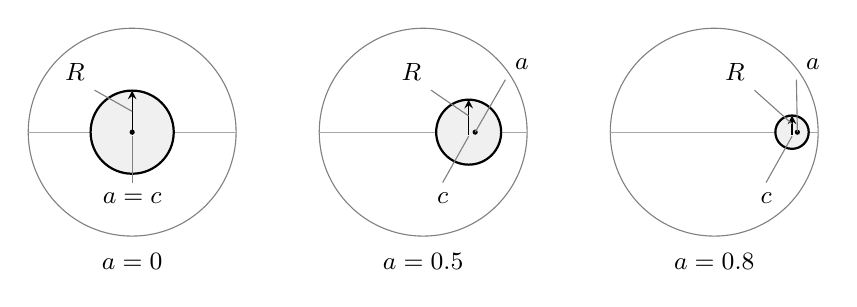
\begin{tikzpicture}[>=stealth,font=\small,scale=1.32]
 \foreach \shift/\a/\c/\rad in {0/0/0/0.4,2.8/0.5/0.4375/0.3125,5.6/0.8/0.74866/0.16043}{
  \begin{scope}[xshift=\shift cm]
   \draw[gray] (0,0) circle (1);
   \draw[gray!70] (-1,0)--(1,0);
   \draw[thick,fill=gray!12] (\c,0) circle (\rad);
   \draw[->] (\c,0)--(\c,\rad);
   \node at (\c-0.55,0.58) (radiuslabel) {\(R\)};
   \draw[gray] (radiuslabel.south east)--(\c,0.5*\rad);
   \draw (\c,-0.025)--(\c,0.025);
   \fill (\a,0) circle (0.025);
   \ifdim\a pt=0pt
    \node at (\c,-0.63) (centerlabel) {\(a=c\)};
    \draw[gray] (centerlabel.north)--(\c,-0.04);
   \else
    \node at (\c-0.25,-0.63) (centerlabel) {\(c\)};
    \draw[gray] (centerlabel.north)--(\c,-0.04);
    \node at (0.95,0.65) (pointlabel) {\(a\)};
    \draw[gray] (pointlabel.south west)--(\a,0);
   \fi
   \node[below] at (0,-1.07) {\(a=\a\)};
  \end{scope}
 }
\end{tikzpicture}
\caption[固定伪双曲半径的球]{三个圆盘都满足 \(\delta(z,a)<2/5\)，按同一欧氏尺度绘制。实心点是内在球心 \(a\)，短标记是欧氏圆心 \(c\)；第一图二者重合。由左向右，内在半径不变，欧氏半径 \(R\) 缩小，圆心差也须由公式而不是目测判断。}
\label{b3:fig:06-pseudohyperbolic-balls}
\end{figure}

\cref{b3:fig:06-pseudohyperbolic-balls}固定的是 \(r=2/5\)，而不是欧氏半径 \(R\)。在每幅图中用 \(\phi_a\) 把实心点送到原点后，小圆盘都变成同一个 \(|w|<2/5\)。

\ProseParagraphBreak

球公式给出它离单位圆的最小欧氏间隙：
\[
 1-|c|-R
 =\frac{(1-|a|)(1-r)}{1+r|a|}.
\]
对固定的 \(a,r\)，这个数为正；当中心趋向边界或半径趋向1时，它可以趋于零。因而每一个这样的闭球都是紧的，并不意味着所有闭球可被某一个共同的圆盘内紧集包住。

\ProseParagraphBreak

由距离不变性，每个圆盘自同构 \(T\) 满足
\[
 T(B_\delta(a,r))=B_\delta(T(a),r).
\]
这里等号的一个包含由 \(T\) 的不变性得到，另一个包含对 \(T^{-1}\) 使用同一性质得到。因此换坐标保留的是伪双曲半径 \(r\)，图中的欧氏半径 \(R\) 可以改变。这也解释了为什么一个自同构能在某点放大欧氏长度，同时仍保持所有伪双曲距离。

给定中心 \(a\) 的伪双曲球半径 \(r\) 增大时，欧氏中心从 \(a\) 沿径向移向0，欧氏半径增大。这不是一个固定圆心的同心圆族，却同样构成邻域基。若 \(a\) 为正实数，球与实轴的交点可直接由 \(|(x-a)/(1-ax)|=r\) 解出：
\[
 x_- =\frac{a-r}{1-ar},\quad x_+=\frac{a+r}{1+ar}.
\]
它们的平均数与半差恰为上面的 \(c,R\)，提供配方公式的另一检验。实轴上的这两个端点以后也是双曲距离计算中最简单的坐标。

\ProseParagraphBreak
这两个端点还可以量化边界附近的形状。若 \(a\in(0,1)\)，则
\[
 a-x_-=\frac{r(1-a^2)}{1-ar},\quad
 x_+-a=\frac{r(1-a^2)}{1+ar}.
\]
朝向右边界的宽度较小。当 \(a\uparrow1\) 而 \(r\) 固定时，
\[
 \frac{R}{1-a}\longrightarrow\frac{2r}{1-r^2},\quad
 \frac{1-x_+}{1-a}\longrightarrow\frac{1-r}{1+r},\quad
 \frac{1-x_-}{1-a}\longrightarrow\frac{1+r}{1-r}.
\]
所以整个小圆盘向边界收缩的尺度与 \(1-a\) 相当，但在以 \(a\) 为原点的圆盘坐标中，它始终是同一个半径 \(r\) 的盘。相反，固定 \(a\) 而令 \(r\uparrow1\) 时，\(c\to0\)、\(R\to1\)，这些球递增穷尽 \(\mathbb D\)。两种极限固定的参数不同，几何结果也不同。

\ProseParagraphBreak

现在可以证明一个容易与“距离有界”混淆的事实。

\Needspace{6\baselineskip}
\begin{proposition}\label{b3:prop:06-pseudohyperbolic-complete}
单位圆盘配备伪双曲距离 \(\delta\) 后是完备度量空间：每个 \(\delta\)-Cauchy 列都在 \(\mathbb D\) 中关于 \(\delta\) 收敛。
\end{proposition}
\begin{proof}
设 \((z_n)\) 是 \(\delta\)-Cauchy 列。取 \(N\)，使 \(m,n\ge N\) 时 \(\delta(z_m,z_n)<1/2\)。固定 \(a=z_N\)，序列尾部便包含在闭球 \(\overline B_\delta(a,1/2)\) 中。由 \cref{b3:prop:06-pseudohyperbolic-ball}，存在 \(\rho<1\)，使这个闭球包含于 \(\{|z|\le\rho\}\)。

由 \(|z_m-z_n|\le2\delta(z_m,z_n)\)，该序列是欧氏 Cauchy 列，故收敛到某个 \(z\in\mathbb C\)。尾部位于上述欧氏闭球，因而极限仍在其中，特别地 \(|z|\le\rho<1\)。再用固定紧盘上的比较式，
\[
 \delta(z_n,z)\le\frac{|z_n-z|}{1-\rho^2}\longrightarrow0
 \quad(n\ge N).
\]
这就是所需的圆盘内极限。
\end{proof}

完备性要求 Cauchy 列具有空间内极限，并不要求距离函数无界。例如取 \(z_n=1-1/n\)，\(n\ge2\)，则欧氏意义下相邻项越来越接近边界，但
\[
 \delta(z_n,z_{2n})=\frac{n}{3n-1}\longrightarrow\frac13.
\]
所以它甚至不是 \(\delta\)-Cauchy 列。这里不能只检查相邻两项的距离；Cauchy 条件要求所有充分晚的两项同时接近。闭球公式保证真正的 \(\delta\)-Cauchy 列最终留在圆盘内部的某个紧集，这正是边界点不会作为遗漏极限出现的原因。

下一节将证明任意圆盘全纯自映射都不增加 \(\delta\)。届时，不变性描述的自同构将成为压缩估计的等号情形，而本节的局部尺度公式将把两点估计转成导数估计。

% !TeX root = ../../Book3.tex
\section{Schwarz–Pick 引理}
\label{b3:sec:0603}

Schwarz 引理处理固定原点的圆盘映射。要比较任意两点，先把一个源点及其像分别送到原点，再对复合函数使用同一引理。撤销坐标后，普通的模估计就变成伪双曲距离压缩，原点导数估计则变成随位置变化的导数界。这两个结论既能判断插值数据是否相容，也能控制有内部不动点的迭代。

\subsection{Schwarz–Pick 估计与两点插值}
\label{b3:subsec:060301}

以下仍记 \(\phi_a(z)=(z-a)/(1-\overline a z)\)，其中 \(a\in\mathbb D\)。前节定义的距离为 \(\delta(z,w)=|\phi_w(z)|\)。\term[schwarz-pick-yinli]{Schwarz--Pick 引理}[Schwarz--Pick lemma]说明，全纯圆盘映射虽然未必压缩欧氏距离，却总压缩这个距离。

\Needspace{6\baselineskip}
\begin{theorem}[Schwarz--Pick]\label{b3:thm:06-schwarz-pick}
设 \(f:\mathbb D\rightarrow\mathbb D\) 全纯。则对所有 \(z,w\in\mathbb D\)，有
\[
 \delta(f(z),f(w))\le\delta(z,w),
 \quad
 \frac{|f'(w)|}{1-|f(w)|^2}\le\frac1{1-|w|^2}.
\]
若在某一点的导数不等式中取等，或在某一对不同点的距离不等式中取等，则 \(f\) 是圆盘自同构。反过来，圆盘自同构在上述所有不等式中都取等。
\end{theorem}
\begin{proof}
固定 \(w\in\mathbb D\)，令
\[
 F=\phi_{f(w)}\circ f\circ\phi_w^{-1}.
\]
两端的分式映射都是圆盘自同构，且 \(\phi_w^{-1}(0)=w\)，故 \(F:\mathbb D\rightarrow\mathbb D\) 全纯并满足 \(F(0)=0\)。Schwarz 引理给出
\[
 |F(\phi_w(z))|\le|\phi_w(z)|.
\]
左端是 \(|\phi_{f(w)}(f(z))|\)，所以这就是距离不等式。

对导数，圆盘自同构的公式给
\[
 \phi_{f(w)}'(f(w))=\frac1{1-|f(w)|^2},
 \quad (\phi_w^{-1})'(0)=1-|w|^2.
\]
于是链式法则与 Schwarz 的原点导数估计给出
\[
 |F'(0)|=
 \frac{|f'(w)|\cdot(1-|w|^2)}{1-|f(w)|^2}\le1.
\]
分母均为正，整理即得所需导数式。

若导数式取等，则 \(|F'(0)|=1\)，Schwarz 等号情形使 \(F\) 为旋转。若距离式对 \(z\ne w\) 取等，则 \(\phi_w(z)\ne0\)，同一等号情形仍使 \(F\) 为旋转。撤销两个自同构，\(f\) 便是圆盘自同构。反方向可分别对 \(f\) 和 \(f^{-1}\) 使用已证不等式，两个相反方向的估计迫使距离和导数处处取等。
\end{proof}

“不同点”的条件使距离等号具有内容；取同一点时，任何函数都会给出 \(0=0\)。常值函数也满足两个压缩式，但不在导数式或不同点的距离式中取等。若起初只有 \(|f|\le1\)，则先用最大模原理区分：\(f\) 要么是模一常值，要么处处落在开圆盘中。模一常值的分母 \(1-|f|^2\) 为零，须直接处理。

\ProseParagraphBreak

固定 \(w\)，把距离式除以 \(|z-w|\)，再令 \(z\rightarrow w\)，也会得到导数式。其分母分别趋于 \(1-|f(w)|^2\) 与 \(1-|w|^2\)。不过，一处导数界本身不会直接给出任意两点的比较；上面的坐标归一化同时控制了整个圆盘中的点值。

\Needspace{6\baselineskip}
\begin{proposition}[固定函数值的导数界]\label{b3:prop:06-value-derivative-bound}
设 \(a\in\mathbb C\)、\(R,M>0\)，\(f:D(a,R)\rightarrow D(0,M)\) 全纯，并记 \(c=f(a)\)。则
\[
 |f'(a)|\le\frac{M^2-|c|^2}{MR}.
\]
对每个 \(c\in D(0,M)\)，都存在具有该中心值并达到导数上界的映射。
\end{proposition}
\begin{proof}
在\eqref{b3:eq:06-center-derivative}中令目标圆心为零、目标半径为 \(M\)，便得所列导数界。为了确定它可以达到，任取 \(|\eta|=1\)，令
\[
 f(z)=M\cdot\phi_{c/M}^{-1}\left(\eta\frac{z-a}{R}\right).
\]
这个映射双全纯到 \(D(0,M)\)，在 \(a\) 取值 \(c\)，导数为 \(\eta(M^2-|c|^2)/(MR)\)，故达到上界。
\end{proof}

例如 \(M=R=1\)、\(a=0\)、\(c=1/2\) 时，导数模至多为 \(3/4\)，而不利用中心值的 Cauchy 估计只给 \(1\)。映射 \((z+1/2)/(1+z/2)\) 在原点的值为 \(1/2\)，导数为 \(3/4\)，说明这个改进是准确的。

\ProseParagraphBreak

两点插值把估计的必要条件变成存在性的完整判据。构造时先把第一组插值数据移到零点，余下只需用一个线性映射把第二个源值送到第二个目标值。

\Needspace{6\baselineskip}
\begin{proposition}[两点插值]\label{b3:prop:06-two-point-interpolation}
给定不同的 \(z_1,z_2\in\mathbb D\) 及 \(w_1,w_2\in\mathbb D\)。存在全纯映射 \(f:\mathbb D\rightarrow\mathbb D\)，使 \(f(z_j)=w_j\)、\(j=1,2\)，当且仅当
\[
 \delta(w_1,w_2)\le\delta(z_1,z_2).
\]
若取等，插值映射唯一，且为圆盘自同构；若严格不等，则有无穷多个不同的插值映射。
\end{proposition}
\begin{proof}
必要性来自 Schwarz--Pick。为证明充分性，令
\[
 p=\phi_{z_1}(z_2),\quad q=\phi_{w_1}(w_2),\quad c=q/p.
\]
源点互异使 \(p\ne0\)，条件又给 \(|c|\le1\)。于是
\[
 f(z)=\phi_{w_1}^{-1}\bigl(c\cdot\phi_{z_1}(z)\bigr)
\]
全纯地将圆盘映入自身，并满足两项插值。当 \(|c|=1\) 时，它是自同构。任何其他解的归一化函数 \(F=\phi_{w_1}\circ f\circ\phi_{z_1}^{-1}\) 满足 \(F(0)=0\)、\(F(p)=q\)。若 \(|q|=|p|\)，Schwarz 等号迫使 \(F(\zeta)=c\zeta\)，所以这个解唯一。

若 \(|c|<1\)，对每个满足
\[
 |t|<\frac{1-|c|}{1+|p|}
\]
的复数 \(t\)，定义 \(H_t(\zeta)=c+t(\zeta-p)\)。对 \(\zeta\in\mathbb D\)，有 \(|H_t(\zeta)|\le|c|+|t|\cdot(1+|p|)<1\)，而 \(H_t(p)=c\)。因此 \(F_t(\zeta)=\zeta\cdot H_t(\zeta)\) 都满足 \(F_t(0)=0\)、\(F_t(p)=q\)。撤销坐标得到插值映射 \(f_t\)。不同的 \(t\) 给出不同的多项式 \(F_t\)，故也给出不同的 \(f_t\)。
\end{proof}

取 \(z_1=w_1=0\)、\(z_2=1/2\)。若要求 \(w_2=3/4\)，目标距离大于源距离，无解；若改为 \(w_2=1/4\)，则 \(f(z)=z/2\) 是一个解；若取 \(w_2=1/2\)，唯一解是恒等映射。对三个点，原始数据的成对距离条件还不够，下一小节将用一次除零点步骤找出剩余的相容条件。

\ProseParagraphBreak

严格压缩不意味着全圆盘共有一个小于 \(1\) 的压缩系数。对 \(f(z)=z^2\)，其归一化导数比为
\[
 \frac{|f'(z)|\cdot(1-|z|^2)}{1-|f(z)|^2}
 =\frac{2|z|}{1+|z|^2}<1.
\]
每个内点都严格小于 \(1\)，但沿 \(|z|\uparrow1\) 趋于 \(1\)。只有固定 \(|z|\le r<1\) 后，才能用 \(2r/(1+r^2)<1\) 作共同上界。

\subsection{不动点迭代与插值构造}
\label{b3:subsec:060302}

圆盘映射若有内部不动点，就可以通过共轭把它移到原点。此时 Schwarz 引理使每条轨道留在一个内部紧盘里，紧盘上的严格性足以证明整条迭代轨道收敛。

\Needspace{6\baselineskip}
\begin{proposition}[内部不动点的刚性]\label{b3:prop:06-two-fixed-points}
设 \(f:\mathbb D\rightarrow\mathbb D\) 全纯。若 \(f\) 固定两个不同的内部点，则 \(f\) 为恒等映射。若 \(a\in\mathbb D\)、\(f(a)=a\) 且 \(f'(a)=1\)，则 \(f\) 也为恒等映射。
\end{proposition}
\begin{proof}
若有两个不同不动点 \(a,b\)，距离不等式在该点对取等，故 \(f\) 是自同构。映射 \(g=\phi_a\circ f\circ\phi_a^{-1}\) 固定零点，所以是旋转 \(g(\zeta)=\eta\zeta\)。它还固定非零点 \(\phi_a(b)\)，故 \(\eta=1\)，撤销共轭即得 \(f=\mathrm{id}\)。

对第二项，同样的共轭满足 \(g(0)=0\)，并由链式法则得到 \(g'(0)=f'(a)=1\)。Schwarz 导数等号给出 \(g(\zeta)=\zeta\)，于是 \(f\) 仍是恒等映射。
\end{proof}

\Needspace{6\baselineskip}
\begin{proposition}[内点不动点处的迭代]\label{b3:prop:06-interior-iteration}
设 \(f:\mathbb D\rightarrow\mathbb D\) 全纯，\(a\in\mathbb D\)，且 \(f(a)=a\)。若 \(f\) 不是圆盘自同构，则迭代 \(f^{\circ n}\) 在 \(\mathbb D\) 上局部一致趋于常值 \(a\)。在已有内部不动点的条件下，\(f\) 不是圆盘自同构等价于 \(|f'(a)|<1\)。
\end{proposition}
\begin{proof}
令 \(g=\phi_a\circ f\circ\phi_a^{-1}\)。它固定零点，且 \(g'(0)=f'(a)\)。Schwarz 引理给 \(|g'(0)|\le1\)，取等当且仅当 \(g\) 为旋转；这也恰是 \(f\) 为圆盘自同构的情形。因此题设等价于 \(|f'(a)|<1\)。

在原点补上导数后，函数 \(h(\zeta)=g(\zeta)/\zeta\) 全纯且 \(|h|\le1\)。若它在某个内点取模 \(1\)，最大模原理使它为单位常数，\(g\) 就成为旋转，与假设矛盾。所以对每个 \(0<r<1\)，都有
\[
 q_r=\max_{|\zeta|\le r}|h(\zeta)|<1.
\]
Schwarz 引理使 \(g\) 把 \(\overline{D(0,r)}\) 映入自身，故可反复使用同一个常数，归纳得到
\[
 |g^{\circ n}(\zeta)|\le q_r^n\cdot|\zeta|
 \quad(|\zeta|\le r).
\]
对原圆盘中的固定紧集 \(K\)，选 \(r<1\) 使 \(\phi_a(K)\subseteq\overline{D(0,r)}\)。因为
\[
 \phi_a^{-1}(u)-a=\frac{(1-|a|^2)u}{1+\overline a u},
\]
共轭关系给出
\[
 \sup_{z\in K}|f^{\circ n}(z)-a|
 \le\frac{1-|a|^2}{1-|a|\cdot r}\,q_r^n r
 \longrightarrow0.
\]
分母为正，且不随 \(n\) 改变，故得到紧集上的一致收敛。
\end{proof}

旋转是这一结论的准确例外。若共轭后的映射为 \(g(\zeta)=\eta\zeta\)、\(|\eta|=1\)，则迭代为 \(\eta^n\zeta\)。当 \(\eta\ne1\) 时，任何非零轨道都不收敛：若极限为 \(L\)，其模非零，而相邻项关系又给 \(L=\eta L\)，矛盾。单位根情形的轨道是周期的；\(\eta=1\) 时则每个点固定。没有内部不动点的映射可能有趋近边界的轨道，那属于后续 Denjoy--Wolff 理论，本处不据此作结论。

\ProseParagraphBreak

例如 \(g(z)=z^2\) 的第 \(n\) 次迭代为 \(z^{2^n}\)，在 \(|z|\le r<1\) 上误差至多 \(r^{2^n}\)，却不在整个开圆盘上一致趋于零，其模的全域上确界始终为 \(1\)。固定紧集使所有迭代点共享一个严格小于 \(1\) 的估计。

\ProseParagraphBreak

把归一化后的零点除去，也能逐步处理插值数据。一次取值条件被消去以后，剩余自由度由另一个模不超过 \(1\) 的全纯函数表示。这称为\term[schur-buzhou]{Schur 步骤}[Schur step]。

\Needspace{6\baselineskip}
\begin{proposition}[Schur 步骤]\label{b3:prop:06-schur-step}
给定 \(c\in\mathbb D\)，令 \(\phi_c(w)=(w-c)/(1-\overline c w)\)。若 \(f:\mathbb D\rightarrow\mathbb D\) 全纯且 \(f(0)=c\)，则
\[
 g(z)=\frac{\phi_c(f(z))}{z}\quad(z\ne0)
\]
在原点可去，补定义后全纯且 \(|g(z)|\le1\)，并有
\[
 g(0)=\frac{f'(0)}{1-|c|^2}.
\]
反过来，对每个在 \(\mathbb D\) 上全纯且模不超过 \(1\) 的函数 \(g\)，公式
\[
 f(z)=\phi_c^{-1}\bigl(z\cdot g(z)\bigr)
     =\frac{c+z\cdot g(z)}{1+\overline c z\cdot g(z)}
\]
定义一个满足 \(f(0)=c\) 的全纯圆盘映射。这两个操作互为逆操作。
\end{proposition}
\begin{proof}
函数 \(\phi_c\circ f\) 固定零点，Schwarz 引理给 \(|\phi_c(f(z))|\le|z|\)。其 Taylor 展开的一次系数为 \(\phi_c'(c)\cdot f'(0)=f'(0)/(1-|c|^2)\)，所以除以 \(z\) 后可去，且原点补值如上。模估计在非零点成立，在原点由连续性成立。

反过来，\(|z\cdot g(z)|\le|z|<1\)，因此即使 \(g\) 是单位常数，乘积也始终落在开圆盘内。分母的模至少为 \(1-|c|\cdot|z|>0\)，复合逆自同构合法，给出全纯圆盘映射及 \(f(0)=c\)。两边施加 \(\phi_c\) 得到 \(\phi_c(f(z))=z\cdot g(z)\)，从而两个操作互逆。
\end{proof}

如果 \(|f'(0)|=1-|c|^2\)，则 \(|g(0)|=1\)，最大模原理迫使 \(g\) 是单位常数，原函数因而是自同构。若 \(|g(0)|<1\)，则 \(g\) 全部取值于开盘，才可继续作下一步。例如 \(f(0)=f'(0)=0\) 时，连续两次 Schwarz 除零点得到 \(|f(z)|\le|z|^2\)；若再有 \(f''(0)=2\eta\)、\(|\eta|=1\)，第二个商被迫恒为 \(\eta\)，所以 \(f(z)=\eta z^2\)。

\Needspace{6\baselineskip}
\begin{proposition}[二阶 Taylor 数据的相容性]\label{b3:prop:06-second-jet}
给定 \(c,d,e\in\mathbb C\)、\(|c|<1\)，记
\[
 A=1-|c|^2,\quad p=\frac dA,\quad
 q=\frac eA+\frac{\overline c d^2}{A^2}.
\]
存在全纯映射 \(f:\mathbb D\rightarrow\mathbb D\)，使其原点展开为
\[
 f(z)=c+dz+ez^2+O(z^3),
\]
当且仅当以下两种情形之一成立：\(|p|<1\) 且 \(|q|\le1-|p|^2\)；或者 \(|p|=1\) 且 \(q=0\)。这里 \(e=f''(0)/2\)。
\end{proposition}
\begin{proof}
先作 Schur 步骤，令 \(g=\phi_c(f)/z\)。为了辨认 \(g\) 的前两项，记 \(t=f-c=dz+ez^2+O(z^3)\)。因为 \(A>0\)，原点附近有
\[
 \begin{aligned}
 \phi_c(f)&=\frac{t}{A-\overline c t}
   =\frac tA+\frac{\overline c}{A^2}t^2+O(z^3)\\
 &=\frac dA z+
   \left(\frac eA+\frac{\overline c d^2}{A^2}\right)z^2+O(z^3).
 \end{aligned}
\]
所以 \(g(z)=p+qz+O(z^2)\)。Schur 步骤给 \(|g|\le1\)，先有 \(|p|\le1\)。若 \(|p|=1\)，最大模原理使 \(g\equiv p\)，故 \(q=0\)。若 \(|p|<1\)，最大模原理排除其他点取模 \(1\)，于是 \(g\) 是开圆盘自映射，Schwarz--Pick 在原点给出 \(|q|\le1-|p|^2\)。这证明了必要性。

为证明充分性，若 \(|p|<1\)，令
\[
 k=\frac q{1-|p|^2},\quad
 g(z)=\phi_p^{-1}(kz)=\frac{p+kz}{1+\overline p kz}.
\]
条件保证 \(|k|\le1\)，所以 \(g\) 把开圆盘映入开圆盘，且 \(g(0)=p\)、\(g'(0)=(1-|p|^2)k=q\)。若 \(|p|=1\)、\(q=0\)，则取 \(g\equiv p\)。两种情形都可以令 \(f=\phi_c^{-1}(zg)\)，Schur 逆步骤保证 \(f:\mathbb D\rightarrow\mathbb D\) 全纯。

还须核对恢复的二阶项。逆分式在零点附近展开为
\[
 \phi_c^{-1}(u)=c+A u-A\overline c u^2+O(u^3).
\]
代入 \(u=z\cdot g(z)=pz+qz^2+O(z^3)\)，得到
\[
 f(z)=c+A pz+A(q-\overline c p^2)z^2+O(z^3).
\]
定义给出 \(Ap=d\)、\(A(q-\overline c p^2)=e\)，因此所构造函数具有全部指定数据。
\end{proof}

当 \(c=0\) 时，条件变成 \(|d|\le1\)、\(|e|\le1-|d|^2\)。例如 \(d=3/4\)、\(e=1/2\) 不相容，因为 \(1/2>7/16\)，尽管两个系数单独都满足 Cauchy 的模上界 \(1\)。当 \(c=1/2\)、\(d=3/4\) 时，第一步已经给 \(p=1\)，于是 \(q=0\) 强制 \(e=-3/8\)。这正是 \((z+1/2)/(1+z/2)\) 的二次系数，显示分式归一化中的 \(\overline c d^2\) 项不可丢掉。

\ProseParagraphBreak

三点插值也能通过一次 Schur 步骤变成两点问题。除零点后出现的指定值可能位于单位圆上，因此需要先处理这个边界情形，再使用开圆盘中的两点判据。

\Needspace{6\baselineskip}
\begin{proposition}[三点插值的 Schur 归约]\label{b3:prop:06-three-point-reduction}
设 \(a_1,a_2,a_3\in\mathbb D\) 两两不同，\(b_1,b_2,b_3\in\mathbb D\)。记 \(\phi_a(z)=(z-a)/(1-\overline a z)\)，并令
\[
 p_j=\phi_{a_1}(a_j),\quad
 q_j=\frac{\phi_{b_1}(b_j)}{p_j}\quad(j=2,3).
\]
存在全纯映射 \(f:\mathbb D\rightarrow\mathbb D\)，使 \(f(a_j)=b_j\)、\(j=1,2,3\)，当且仅当以下之一成立：\(q_2,q_3\in\mathbb D\) 且 \(\delta(q_2,q_3)\le\delta(p_2,p_3)\)；或者 \(q_2=q_3\) 且 \(|q_2|=1\)。
\end{proposition}
\begin{proof}
源点互异使 \(p_2,p_3\) 非零且不同，故各商有定义。若插值映射存在，则
\[
 G=\phi_{b_1}\circ f\circ\phi_{a_1}^{-1}
\]
是固定零点的圆盘映射。Schur 步骤使 \(H(\zeta)=G(\zeta)/\zeta\) 在零点可去，且 \(|H|\le1\)。插值条件等价于 \(H(p_j)=q_j\)、\(j=2,3\)。如果某个 \(|q_j|>1\)，便不可能；如果某个 \(|q_j|=1\)，最大模原理迫使 \(H\) 恒为这个单位数，所以另一个 \(q_j\) 必须相同。剩下 \(q_2,q_3\in\mathbb D\) 的情形，\(H\) 也处处在开盘内，两点插值判据给出所列距离条件。

反过来，若 \(q_2=q_3\) 为单位数，取 \(H\equiv q_2\)。若两值都在开盘且满足距离条件，可以明确取
\[
 k=\frac{\phi_{q_2}(q_3)}{\phi_{p_2}(p_3)},
 \quad H(\zeta)=\phi_{q_2}^{-1}\bigl(k\cdot\phi_{p_2}(\zeta)\bigr).
\]
因为 \(p_2\ne p_3\)，分母非零，而条件给 \(|k|\le1\)。这就是两点命题中的构造，满足 \(H(p_j)=q_j\)。两种情形均可定义
\[
 f(z)=\phi_{b_1}^{-1}\Bigl(
       \phi_{a_1}(z)\cdot H\bigl(\phi_{a_1}(z)\bigr)\Bigr).
\]
乘积的模严格小于 \(1\)，包括 \(H\) 为单位常数的情形，故所得函数全纯且取值于开盘。在 \(a_1\) 处乘积为零；在另外两点处，它等于 \(p_jq_j=\phi_{b_1}(b_j)\)。代入逆分式就恢复全部三项插值。
\end{proof}

若约化函数被迫为单位常数，或最后两点的距离不等式取等，约化后的 \(H\) 唯一，原映射也唯一。若最后两点严格不等，前面的构造给出无穷多个不同的 \(H\)，逆步骤也给出不同的原映射。

\ProseParagraphBreak

例如要求 \(f(0)=0\)、\(f(1/2)=f(-1/2)=2/5\)。每一对原始数据都满足 Schwarz--Pick：中心到另外两点的目标距离为 \(2/5<1/2\)，后两个目标之间的距离为零。但除去已知零点后，\(H=f/z\) 必须在 \(1/2,-1/2\) 分别取值 \(4/5,-4/5\)。这不可能，因为
\[
 \delta(4/5,-4/5)=\frac{40}{41}
 >\frac45=\delta(1/2,-1/2).
\]
共同的 Schur 归约揭示了各点数据之间的额外约束，不能把不同点对各自存在的解直接拼接。

\subsection{等号刚性与正实部估计}
\label{b3:subsec:060303}

内部的精确等号已经迫使映射成为自同构；若导数只是接近极值，还可以量化函数在紧集上离极端映射有多远。设 \(f:\mathbb D\rightarrow\mathbb D\) 全纯，\(f(0)=0\)，且 \(f'(0)=a\in[0,1]\)。当 \(a<1\) 时，商 \(h=f/z\) 补定义后满足 \(h(0)=a\)、\(|h|<1\)。Schwarz--Pick 给 \(\delta(h(z),a)\le|z|\)。固定 \(0<r<1\)，对 \(|z|\le r\) 有
\[
 \begin{aligned}
 |h(z)-a|&\le r\cdot|1-ah(z)|\\
 &\le r\bigl(1-a^2+a\cdot|h(z)-a|\bigr).
 \end{aligned}
\]
因为 \(1-ar>0\)，移项给出 \(|h-a|\le r(1-a^2)/(1-ar)\)。再由 \(|f(z)-z|\le|z|\cdot(|h(z)-a|+1-a)\)，得到
\[
 \sup_{|z|\le r}|f(z)-z|
 \le\frac{r(1-a)(1+r)}{1-ar}.
\]
若 \(a=1\)，Schwarz 等号直接给 \(f=z\)，同一上界仍成立。因此归一化导数趋于 \(1\) 时，函数在每个固定紧盘上一致趋于恒等。对非零复导数，可先旋转函数使导数正实，再与相应旋转映射比较。

\ProseParagraphBreak

把右半平面映到圆盘，还能将正实部条件转成模约束。这个转换保留的信息比一般的模有界条件更强，因为实部的正性同时控制了圆周平均值和各阶系数。

\Needspace{6\baselineskip}
\begin{proposition}[正实部函数的增长估计]\label{b3:prop:06-positive-real-part}
设 \(p:\mathbb D\rightarrow\mathbb C\) 全纯，\(\operatorname{Re}p(z)>0\) 对全部 \(z\in\mathbb D\) 成立，且 \(p(0)=1\)。则对每个 \(z\in\mathbb D\)，记 \(r=|z|\)，有
\[
 \frac{1-r}{1+r}\le\operatorname{Re}p(z)
 \le\frac{1+r}{1-r},
 \quad |p(z)|\le\frac{1+r}{1-r}.
\]
\end{proposition}
\begin{proof}
正实部使 \(p+1\) 无零，且
\[
 |p+1|^2-|p-1|^2=4\operatorname{Re}p>0.
\]
所以 \(q=(p-1)/(p+1)\) 是圆盘映射，\(q(0)=0\)，Schwarz 引理给 \(|q(z)|\le r\)。反解 \(p=(1+q)/(1-q)\)，得到
\[
 \operatorname{Re}p(z)=\frac{1-|q(z)|^2}{|1-q(z)|^2}.
\]
令 \(s=|q(z)|\le r\)。由 \(1-s\le|1-q(z)|\le1+s\)，有
\[
 \frac{1-s}{1+s}\le\operatorname{Re}p(z)\le\frac{1+s}{1-s},
 \quad |p(z)|\le\frac{1+s}{1-s}.
\]
左侧函数随 \(s\) 递减，右侧函数随 \(s\) 递增，代入 \(s\le r\) 即得全部估计。
\end{proof}

函数 \(p_\eta(z)=(1+\eta z)/(1-\eta z)\)、\(|\eta|=1\)，在满足 \(\eta z=r\) 的点达到上界，在满足 \(\eta z=-r\) 的点达到实部下界。因此两个方向的界都可达到。这里的推导只对全纯函数的实部进行，后面的调和函数理论将解释同样的 Harnack 因子。

\ProseParagraphBreak

\term[caratheodory-xishu-budengshi]{Carathéodory 系数不等式}[Carathéodory coefficient inequality]进一步给出与阶数无关的系数界。

\Needspace{6\baselineskip}
\begin{proposition}[Carathéodory 系数估计]\label{b3:prop:06-caratheodory-coefficients}
设 \(p:\mathbb D\rightarrow\mathbb C\) 全纯，\(\operatorname{Re}p>0\)、\(p(0)=1\)，且
\[
 p(z)=1+\sum_{n=1}^{\infty}c_nz^n.
\]
则每个整数 \(n\ge1\) 都满足 \(|c_n|\le2\)。
\end{proposition}
\begin{proof}
固定 \(0<r<1\)，记 \(u(t)=\operatorname{Re}p(re^{\mathrm{i}t})>0\)。Taylor 级数在这一固定圆周上一致收敛，故可取实部，写为
\[
 u(t)=1+\frac12\sum_{m=1}^{\infty}
 \left(c_mr^me^{\mathrm{i}mt}+\overline{c_m}r^me^{-\mathrm{i}mt}\right).
\]
对这个一致收敛级数逐项积分，利用非零整数频率的指数在一周上的积分为零，得到
\[
 \frac1{2\pi}\int_0^{2\pi}u(t)\,\mathrm{d}t=1,
 \quad
 \frac1{2\pi}\int_0^{2\pi}u(t)\cdot e^{-\mathrm{i}nt}\,\mathrm{d}t
 =\frac12c_nr^n\quad(n\ge1).
\]
因为 \(u(t)>0\) 且 \(|e^{-\mathrm{i}nt}|=1\)，带振荡因子的积分模不超过 \(u\) 的积分。因此 \(|c_n|\cdot r^n\le2\)。对固定 \(n\) 令 \(r\uparrow1\)，得到 \(|c_n|\le2\)。整个论证只在内部圆周上积分，不需要 \(p\) 在单位圆上具有边界值。
\end{proof}

上面的极端函数还有展开
\[
 \frac{1+\eta z}{1-\eta z}
 =1+2\sum_{n=1}^{\infty}\eta^nz^n\quad(|\eta|=1),
\]
所有非恒定系数的模均为 \(2\)，所以每个阶数都达到同一界。若全纯函数 \(p(z)=c_0+\sum_{n\ge1}c_nz^n\) 仍满足 \(\operatorname{Re}p>0\)，但常数项任意，令 \(\alpha=\operatorname{Re}c_0>0\)、\(\beta=\operatorname{Im}c_0\)。归一化函数 \((p-\mathrm{i}\beta)/\alpha\) 满足前一命题，故一般形式为 \(|c_n|\le2\operatorname{Re}c_0\)、\(n\ge1\)。常数项的虚部不参与这个约束。

\subsection{共形映射下的转移}
\label{b3:subsec:060304}

对真单连通区域，Riemann 映照提供全局圆盘坐标。先把距离和局部尺度转回原区域，并证明它们不依赖坐标选择，就能将 Schwarz--Pick 写成区域本身的结论。

\Needspace{6\baselineskip}
\begin{definition}[区域上的距离与密度]\label{b3:def:06-conformal-transfer}
设 \(U\subsetneq\mathbb C\) 为单连通区域，\(\Phi:U\rightarrow\mathbb D\) 为双全纯映射。对 \(z,w\in U\)，定义
\[
 \delta_U(z,w)\coloneqq\delta(\Phi(z),\Phi(w)),
 \quad
 \lambda_U(z)\coloneqq\frac{2|\Phi'(z)|}{1-|\Phi(z)|^2}.
\]
分别称为 \(U\) 上的伪双曲距离和\term[poincare-midu]{Poincaré 密度}[Poincaré density]。
\end{definition}
\symidx{\(\delta_U(z,w)\)：真单连通区域上的伪双曲距离}
\symidx{\(\lambda_U(z)\)：Poincaré 密度}

这两个定义与 \(\Phi\) 的选择无关。若另一坐标为 \(\Psi\)，则 \(A=\Psi\circ\Phi^{-1}\) 是圆盘自同构，前节的不变性给出 \(\delta(Au,Av)=\delta(u,v)\)。同时，自同构的导数恒等式为
\[
 \frac{|A'(u)|}{1-|A(u)|^2}=\frac1{1-|u|^2}.
\]
代入 \(u=\Phi(z)\) 并使用链式法则，便得用 \(\Psi\) 和用 \(\Phi\) 计算的 \(\lambda_U\) 相同。距离的度量性质由双射 \(\Phi\) 和 \(\delta\) 的性质传回；密度则处处为正，因为双全纯映射的导数不为零。

\ProseParagraphBreak

密度与上一章的共形半径可以在基点处直接比较。对固定 \(a\in U\)，选择满足 \(\Phi(a)=0\)、\(\Phi'(a)>0\) 的归一化坐标，得到
\[
 \lambda_U(a)=2\Phi'(a)=\frac2{r_U(a)}.
\]
坐标无关性保证这个等式对每个基点都成立。

\Needspace{6\baselineskip}
\begin{proposition}[单连通区域上的 Schwarz--Pick 估计]\label{b3:prop:06-conformal-schwarz-pick}
设 \(U,V\subsetneq\mathbb C\) 为单连通区域，\(f:U\rightarrow V\) 全纯。则对所有 \(z,w\in U\)，有
\[
 \delta_V(f(z),f(w))\le\delta_U(z,w),
 \quad \lambda_V(f(z))\cdot|f'(z)|\le\lambda_U(z).
\]
若在一对不同点的距离式中取等，或在某一点的导数式中取等，则 \(f\) 双全纯映满 \(V\)。反过来，双全纯映射在这些式子中处处取等。
\end{proposition}
\begin{proof}
取圆盘坐标 \(\Phi_U:U\rightarrow\mathbb D\)、\(\Phi_V:V\rightarrow\mathbb D\)，并令 \(G=\Phi_V\circ f\circ\Phi_U^{-1}\)。圆盘的 Schwarz--Pick 距离式直接变成所需的距离式。对 \(a\in U\)，在 \(\zeta=\Phi_U(a)\) 处有
\[
 G'(\zeta)=\frac{\Phi_V'(f(a))\cdot f'(a)}{\Phi_U'(a)}.
\]
将它代入圆盘导数式，再乘以正数 \(2|\Phi_U'(a)|\)，便得到 \(\lambda_V(f(a))\cdot|f'(a)|\le\lambda_U(a)\)。这里坐标导数均非零，所有分母为正，所以等号也准确对应。圆盘中的等号迫使 \(G\) 为自同构，故 \(f=\Phi_V^{-1}\circ G\circ\Phi_U\) 双全纯映满 \(V\)。反向同样由圆盘自同构的等号性质得到。
\end{proof}

用共形半径改写导数式，就是
\[
 \frac{|f'(a)|}{r_V(f(a))}\le\frac1{r_U(a)}.
\]
若 \(U\subseteq V\)，对恒等嵌入应用此式，得到 \(r_U(a)\le r_V(a)\)；一处取等就迫使恒等嵌入满射，所以只能有 \(U=V\)。这也恢复了上一章共形半径的严格单调性。

\ProseParagraphBreak

在右半平面 \(H_R=\{\,z\in\mathbb C\mid\operatorname{Re}z>0\,\}\)，取 \(\Phi(z)=(z-1)/(z+1)\)。由
\[
 |\Phi'(z)|=\frac2{|z+1|^2},
 \quad 1-|\Phi(z)|^2=\frac{4\operatorname{Re}z}{|z+1|^2},
\]
可得 \(\lambda_{H_R}(z)=1/\operatorname{Re}z\)。因此每个全纯映射 \(F:\mathbb D\rightarrow H_R\) 满足
\[
 \frac{|F'(z)|}{\operatorname{Re}F(z)}\le\frac2{1-|z|^2}.
\]
若 \(F(0)=1\)，距离式还给 \(|(F(z)-1)/(F(z)+1)|\le|z|\)，正是前面正实部估计所使用的圆盘约束。

\ProseParagraphBreak

在上半平面 \(\mathbb H=\{\,z\in\mathbb C\mid\operatorname{Im}z>0\,\}\)，同样用 \((z-\mathrm{i})/(z+\mathrm{i})\) 计算，得到
\[
 \delta_{\mathbb H}(z,w)=\left|\frac{z-w}{z-\overline w}\right|,
 \quad \lambda_{\mathbb H}(z)=\frac1{\operatorname{Im}z}.
\]
于是全纯映射 \(F:\mathbb H\rightarrow\mathbb H\) 满足
\[
 \left|\frac{F(z)-F(w)}{F(z)-\overline{F(w)}}\right|
 \le\left|\frac{z-w}{z-\overline w}\right|,
 \quad \frac{|F'(z)|}{\operatorname{Im}F(z)}\le\frac1{\operatorname{Im}z}.
\]
例如 \(F(z)=z+\mathrm{i}\) 的欧氏导数为 \(1\)，但 \(\operatorname{Im}F(z)=\operatorname{Im}z+1\)，所以密度导数式严格压缩。若 \(F(z)=(az+b)/(cz+d)\)，其中 \(a,b,c,d\) 为实数、\(ad-bc>0\)，则
\[
 \operatorname{Im}F(z)=\frac{(ad-bc)\operatorname{Im}z}{|cz+d|^2}.
\]
它及其分式逆都保持上半平面，故为自同构，在两个估计中均取等。

\ProseParagraphBreak

本小节的全局圆盘坐标依赖真单连通条件。对有孔区域，局部坐标不能直接拼成一个双全纯圆盘映射，推广密度需要后面的覆盖理论。\chapref{b3:ch:13}还将用 \(\lambda_U(z)\cdot|\mathrm{d}z|\) 定义曲线长度，再由长度下确界构造 Poincaré 距离；这里的 \(\delta_U\) 与那个路径距离是不同的数值。


\begin{chaptersummary}
本章反复使用同一个归一化方法：先把指定的源点和像点送到0，再对所得圆盘映射应用 Schwarz 引理。撤销坐标后，函数值的比较成为伪双曲距离压缩，导数的比较则带上源、目标两处的密度因子。伪双曲距离虽小于1，仍是真正的度量；其球的欧氏大小随位置变化，固定内部紧集上的欧氏比较不能直接推广到圆盘边缘。

\ProseParagraphBreak

精确等号与定量压缩承担不同任务。一对不同内点或一个内点导数的等号迫使自同构；非自同构给逐点严格不等式，却未必给全域共有的小于1的系数。有限零点除法与 Schur 步骤把这一思想用于系数和插值：先化去已给数据，再检查剩余函数是否仍满足圆盘约束，最后反向构造。正实部问题通过 Cayley 变换接入同一方法。换到一般真单连通区域时，距离与密度不依赖所选圆盘坐标；显式的半平面和条带计算说明这种不变性怎样变成可用的尺度估计。
\end{chaptersummary}

\BookExercises

% 本章8题均为自拟；以已有工具增加边界尺度、球几何、插值构造和显式迭代训练。
\Needspace{6\baselineskip}
\begin{exercise}\label{b3:ex:06-1}
对 \(0<r<1\)，计算 \(\delta(r,-r)\) 与 \(\delta(0,r)\)，比较它们与对应的欧氏距离。再固定 \(\alpha,\beta>0\)，令
\[
 z_\varepsilon=1-\alpha\varepsilon,\quad
 w_\varepsilon=1-\beta\varepsilon
\]
在充分小的 \(\varepsilon>0\) 时位于单位圆盘内，求 \(\delta(z_\varepsilon,w_\varepsilon)\) 的极限。最后考察 \(z_n=1-1/n\)、\(w_n=1-1/n^2\)，说明两个点即使趋于同一个边界点、欧氏距离趋于0，伪双曲距离也可能趋于1。
\end{exercise}
\begin{solution}
由定义直接得到
\[
 \delta(r,-r)=\frac{2r}{1+r^2},
 \quad
 \delta(0,r)=r.
\]
对应的欧氏距离是 \(2r\) 与 \(r\)。第一组中伪双曲距离小于欧氏距离，两组伪双曲距离都在 \(r\uparrow1\) 时趋于1；这些计算并不说明在所有位置都能用欧氏距离给统一的上界。

取 \(0<\varepsilon<1/\max\{\alpha,\beta\}\)，两个点均为 \((0,1)\) 中的实数，且
\[
 1-z_\varepsilon w_\varepsilon
 =(\alpha+\beta)\varepsilon-\alpha\beta\varepsilon^2>0.
\]
于是
\[
 \delta(z_\varepsilon,w_\varepsilon)
 =\frac{|\alpha-\beta|}{\alpha+\beta-\alpha\beta\varepsilon}
 \longrightarrow\frac{|\alpha-\beta|}{\alpha+\beta}.
\]
若 \(\alpha\ne\beta\)，极限为正，而欧氏距离
\(|z_\varepsilon-w_\varepsilon|=|\alpha-\beta|\varepsilon\) 趋于0。因此不存在一个对全单位圆盘有效的有限常数 \(C\)，使 \(\delta(z,w)\le C|z-w|\) 对全部点成立。这里两点离边界的距离具有同一阶，极限记录的是两个尺度的比值。

若靠近边界的速度不同，距离还能更大。对 \(n\ge2\)，
\[
 \delta(z_n,w_n)
 =\frac{1/n-1/n^2}{1/n+1/n^2-1/n^3}
 =\frac{n^2-n}{n^2+n-1}\longrightarrow1.
\]
与此同时，\(|z_n-w_n|=1/n-1/n^2\to0\)，且两点都趋于1。伪双曲距离所保留的分母与两点各自的边界尺度有关，不能只凭欧氏图上的靠近判断其极限。
\end{solution}

\Needspace{6\baselineskip}
\begin{exercise}\label{b3:ex:06-2}
不直接套用一般球公式，从不等式出发求
\[
 B=\{\,z\in\mathbb D\mid\delta(z,1/2)<1/2\,\}
\]
的欧氏中心、半径及与实轴的交点。用自同构 \(\phi_{1/2}\) 解释这两个端点，并求闭球 \(\overline B\) 到单位圆周的最短欧氏距离。说明为什么伪双曲球心 \(1/2\) 不是这个欧氏圆盘的中心。
\end{exercise}
\begin{solution}
令 \(z=x+\mathrm{i}y\)。由于 \(1-z/2\ne0\)，球条件等价于
\[
 |z-1/2|^2<\frac14|1-z/2|^2.
\]
两边展开并移项，得到
\[
 \frac{15}{16}(x^2+y^2)-\frac34x<0,
\]
再除以首项系数并配方：
\[
 \left(x-\frac25\right)^2+y^2<\left(\frac25\right)^2.
\]
因此欧氏圆心为 \(2/5\)，半径为 \(2/5\)。这个圆盘确实包含于单位圆盘，因为其闭包上的 \(|z|\) 至多为 \(4/5<1\)。它与实轴的交集为 \((0,4/5)\)，两个边界端点为0和 \(4/5\)。

从自同构看，\(\phi_{1/2}\) 把 \(B\) 送到 \(|\zeta|<1/2\)，并把内在球心 \(1/2\) 送到0。它的逆式是
\[
 \phi_{1/2}^{-1}(\zeta)=\frac{\zeta+1/2}{1+\zeta/2}.
\]
代入 \(\zeta=-1/2\) 和 \(\zeta=1/2\)，分别得到0和 \(4/5\)。所以两个实轴端点是同一条直径两端的逆像。分式映射不保持欧氏中点：它们的中点为 \(2/5\)，而0在逆映射下的像为 \(1/2\)。从 \(1/2\) 到两端的欧氏距离分别为 \(1/2\) 与 \(3/10\)，但两端到 \(1/2\) 的伪双曲距离都为 \(1/2\)。

对单位圆盘内任意点 \(z\)，它到单位圆周的欧氏距离是 \(1-|z|\)。闭球中最大的 \(|z|\) 为 \(4/5\)，在正实点 \(4/5\) 达到。因此闭球到单位圆周的最短距离为
\[
 1-\frac45=\frac15,
\]
由 \(4/5\) 与1这对点实现。计算这个正间隙，也就具体核对了该闭伪双曲球是单位圆盘内的紧集。
\end{solution}

\Needspace{6\baselineskip}
\begin{exercise}\label{b3:ex:06-3}
设 \(f:\mathbb D\rightarrow\mathbb D\) 全纯，且
\[
 f(z)=\frac12+\frac12z+ez^2+O(z^3).
\]
求全部允许的二次系数 \(e\in\mathbb C\)，通过 Schur 步骤给出每个允许值对应函数的构造，并证明当 \(e\) 位于允许系数域的边界上时，满足这些数据的函数唯一。
\end{exercise}
\begin{solution}
先将常数项送到0，再除去原点零点：
\[
 g(z)=\frac1z\cdot\frac{f(z)-1/2}{1-f(z)/2}.
\]
Schwarz 引理说明该式在0可去，且 \(|g|\le1\)。为确定留下的数据，实际展开分式：
\[
 \frac{f(z)-1/2}{1-f(z)/2}
 =\frac{\frac12z+ez^2+O(z^3)}
        {\frac34-\frac14z-\frac12ez^2+O(z^3)}
 =\frac23z+\left(\frac43e+\frac29\right)z^2+O(z^3).
\]
所以
\[
 g(0)=\frac23,\quad g'(0)=q=\frac43e+\frac29.
\]
由于 \(g(0)\) 在开圆盘内，最大模原理排除单位常数情形，故 \(g:\mathbb D\to\mathbb D\)。原点处的 Schwarz--Pick 导数式给
\[
 |q|\le1-\frac49=\frac59.
\]
这等价于
\[
 \left|e+\frac16\right|\le\frac5{12}.
\]
可见允许系数域是一个以 \(-1/6\) 为中心的闭圆盘，而不是以0为中心的独立 Cauchy 系数界。

反过来，给定满足该条件的 \(e\)，置
\[
 \kappa=\frac95q=\frac{12e+2}{5},\quad |\kappa|\le1,
\]
并定义
\[
 g_\kappa(z)=\frac{2/3+\kappa z}{1+(2/3)\kappa z},
 \quad
 f_\kappa(z)=\frac{1/2+zg_\kappa(z)}{1+(1/2)zg_\kappa(z)}.
\]
第一式是 \(\phi_{2/3}^{-1}(\kappa z)\)，故它把单位圆盘映入自身，分母不为零。于是 \(|zg_\kappa(z)|<1\)，第二个逆自同构也始终合法，给出 \(f_\kappa:\mathbb D\to\mathbb D\)。其展开为
\[
 g_\kappa(z)=\frac23+\frac59\kappa z+O(z^2),
 \quad
 f_\kappa(z)=\frac12+\frac12z+
 \left(\frac5{12}\kappa-\frac16\right)z^2+O(z^3).
\]
由 \(\kappa\) 的选择，二次项恰为所给 \(e\)，所以闭圆盘内的每一点都确实可实现，包括边界。

若 \(e\) 在边界上，则 \(|q|=5/9\)，即 \(g\) 在原点的 Schwarz--Pick 导数估计取等。令 \(G=\phi_{2/3}\circ g\)，则 \(G(0)=0\)、\(G'(0)=9q/5=\kappa\)，其中 \(|\kappa|=1\)。Schwarz 等号情形迫使 \(G(z)=\kappa z\)，从而 \(g=g_\kappa\)，再反解得 \(f=f_\kappa\)。边界系数的唯一性来自这个精确等号，而不是由有限个 Taylor 系数本身决定一般全纯函数。
\end{solution}

\Needspace{6\baselineskip}
\begin{exercise}\label{b3:ex:06-4}
给定 \(0<r<1\) 和 \(b\in\mathbb C\)，判断是否存在全纯映射 \(f:\mathbb D\rightarrow\mathbb D\)，满足
\[
 f(0)=0,\quad f(r)=f(-r)=b.
\]
证明精确条件为 \(|b|\le r^2\)，构造全部允许数据的一个解，并证明边界情形 \(|b|=r^2\) 的解唯一。实数 \(b\) 的两个端点应分别对应什么函数？
\end{exercise}
\begin{solution}
如果存在解，则 \(b\in\mathbb D\)。将目标值 \(b\) 送到0，令
\[
 h(z)=\phi_b(f(z))=\frac{f(z)-b}{1-\overline b f(z)}.
\]
它把单位圆盘映入自身，且在 \(r,-r\) 处为零。应用有限零点除法，商
\[
 Q(z)=\frac{h(z)}{\phi_r(z)\phi_{-r}(z)}
\]
在这两点可去，并在整个圆盘满足 \(|Q|\le1\)。在0处，
\[
 h(0)=-b,\quad
 \phi_r(0)\phi_{-r}(0)=-r^2,\quad
 Q(0)=\frac b{r^2}.
\]
因此 \(|b|\le r^2\)。这两个零点同时约束同一个商函数，比逐对检查原始三个取值更强。

若 \(|b|\le r^2\)，直接取
\[
 f(z)=\frac b{r^2}z^2.
\]
因为 \(|f(z)|\le|z|^2<1\)，它是合法圆盘映射，并满足全部三项数据。这证明条件充分。

若 \(|b|=r^2\)，记 \(\eta=b/r^2\)，则 \(|\eta|=1\) 且 \(Q(0)=\eta\)。最大模原理使 \(Q\equiv\eta\)。写
\[
 B(z)=\phi_r(z)\phi_{-r}(z)
     =\frac{z^2-r^2}{1-r^2z^2},
\]
便有 \(\phi_b(f)=\eta B\)。由于 \(b=\eta r^2\)，反解并约分得到
\[
 f(z)=\frac{b+\eta B(z)}{1+\overline b\eta B(z)}
     =\eta\frac{r^2+B(z)}{1+r^2B(z)}
     =\eta z^2.
\]
所以边界情形只有这一解。特别地，实数 \(b\) 的允许范围是 \([-r^2,r^2]\)，两端的唯一解分别为 \(-z^2\) 与 \(z^2\)。这也说明三点取值恰好达到兼容性边界时，原本的全纯自由度可以完全消失。
\end{solution}

\Needspace{6\baselineskip}
\begin{exercise}\label{b3:ex:06-5}
给定 \(c_1,c_2\in\mathbb C\)，证明存在单位圆盘上的全纯函数
\[
 p(z)=1+c_1z+c_2z^2+O(z^3),\quad \operatorname{Re}p(z)>0,
\]
当且仅当
\[
 \left|c_2-\frac{c_1^2}{2}\right|
 \le2-\frac{|c_1|^2}{2}.
\]
给出满足条件时的构造，单独处理 \(|c_1|=2\) 的情形，并说明这一兼容条件比分别要求 \(|c_1|,|c_2|\le2\) 更强。
\end{exercise}
\begin{solution}
若 \(p\) 存在，令 \(q=(p-1)/(p+1)\)。正实部条件使 \(p+1\ne0\) 且 \(|q|<1\)，又有 \(q(0)=0\)。幂级数除法给
\[
 q(z)=\frac{c_1}{2}z+
 \left(\frac{c_2}{2}-\frac{c_1^2}{4}\right)z^2+O(z^3).
\]
记
\[
 \alpha=\frac{c_1}{2},\quad
 \beta=\frac{c_2}{2}-\frac{c_1^2}{4}.
\]
商 \(H=q/z\) 在0可去，满足 \(|H|\le1\)、\(H(0)=\alpha\)、\(H'(0)=\beta\)。若 \(|\alpha|<1\)，最大模原理使 \(H\) 映入开圆盘，Schwarz--Pick 给
\(|\beta|\le1-|\alpha|^2\)。若 \(|\alpha|=1\)，则 \(H\) 恒为 \(\alpha\)，故 \(\beta=0\)，同一不等式仍成立。把该不等式乘以2，正是题设条件。

反过来，题设右端必须非负，所以 \(|c_1|\le2\)。若 \(|\alpha|<1\)，置
\[
 \kappa=\frac{\beta}{1-|\alpha|^2},\quad |\kappa|\le1,\quad
 H(z)=\frac{\alpha+\kappa z}{1+\overline\alpha\kappa z}.
\]
这是 \(\phi_\alpha^{-1}(\kappa z)\)，故全纯并取值于开圆盘，且 \(H(0)=\alpha\)、\(H'(0)=\beta\)。令
\[
 q(z)=zH(z),\quad p(z)=\frac{1+q(z)}{1-q(z)}.
\]
由于 \(|q(z)|<1\)，分母不为零，并有
\[
 \operatorname{Re}p(z)
 =\frac{1-|q(z)|^2}{|1-q(z)|^2}>0.
\]
展开 \(q=\alpha z+\beta z^2+O(z^3)\) 后，
\[
 p(z)=1+2\alpha z+2(\beta+\alpha^2)z^2+O(z^3),
\]
恰好恢复 \(c_1,c_2\)，证明了充分性。

若 \(|c_1|=2\)，则 \(|\alpha|=1\)，条件强制 \(\beta=0\)，亦即 \(c_2=c_1^2/2\)。此时只能取 \(H\equiv\alpha\)，所以唯一可能的函数为
\[
 p(z)=\frac{1+\alpha z}{1-\alpha z}.
\]
它在圆盘有正实部，故这一端点情形也可实现。

兼容条件已经蕴含 \(|c_1|\le2\)，并且
\[
 |c_2|
 \le\left|c_2-\frac{c_1^2}{2}\right|+\frac{|c_1|^2}{2}
 \le2.
\]
反向不成立。例如 \(c_1=2,c_2=0\) 分别满足两个模上界，却使兼容不等式左端为2、右端为0。两个系数必须经过同一个 Cayley 变换和同一个有界商函数来实现，不能各自任取一个符合单独上界的数。
\end{solution}

\Needspace{6\baselineskip}
\begin{exercise}\label{b3:ex:06-6}
设 \(F_t(z)=z+\mathrm{i}t\) 作用于上半平面 \(\mathbb H\)，其中 \(t>0\)。计算第 \(n\) 次迭代及其密度压缩比
\[
 \frac{\lambda_{\mathbb H}(F_t^{\circ n}(z))
       \cdot|(F_t^{\circ n})'(z)|}{\lambda_{\mathbb H}(z)}.
\]
比较该比值在固定紧集与整个半平面上的行为，并判断迭代是否球面局部一致或全域一致收敛。再用 \(C(z)=(z-\mathrm{i})/(z+\mathrm{i})\) 转到单位圆盘，写出共轭映射及其迭代，判断其欧氏收敛是否在整个开圆盘一致。
\end{exercise}
\begin{solution}
逐次相加得到
\[
 F_t^{\circ n}(z)=z+n\mathrm{i}t,\quad
 (F_t^{\circ n})'(z)=1.
\]
写 \(z=x+\mathrm{i}y\)，其中 \(y>0\)。上半平面密度为 \(\lambda_{\mathbb H}(z)=1/y\)，所以所求比值等于
\[
 \frac{y}{y+nt}.
\]
它在每个内点严格小于1。若 \(K\subset\mathbb H\) 为固定紧集，取 \(M=\max_K\operatorname{Im}z\)，则
\[
 \sup_{z\in K}\frac{\operatorname{Im}z}{\operatorname{Im}z+nt}
 \le\frac{M}{M+nt}\longrightarrow0.
\]
但对每个固定 \(n\)，令 \(y\to\infty\) 可使比值任意接近1，因此全半平面的上确界仍为1。逐点严格压缩没有给出一个控制全半平面的严格收缩常数。

同时，\(|F_t^{\circ n}(z)|\ge y+nt>nt\)，故
\[
 \chi(F_t^{\circ n}(z),\infty)
 =\frac1{\sqrt{1+|F_t^{\circ n}(z)|^2}}
 \le\frac1{\sqrt{1+n^2t^2}}.
\]
上界与 \(z\) 无关，因此迭代在全半平面球面一致趋于无穷，当然也局部一致。它没有有限值的局部极限，也没有内部不动点。

现在用 \(C^{-1}(\zeta)=\mathrm{i}(1+\zeta)/(1-\zeta)\) 计算共轭。代入并通分得
\[
 g_t(\zeta)=C\circ F_t\circ C^{-1}(\zeta)
 =\frac{t+(2-t)\zeta}{2+t-t\zeta}.
\]
共轭保持复合，故
\[
 g_t^{\circ n}(\zeta)
 =\frac{nt+(2-nt)\zeta}{2+nt-nt\zeta}.
\]
这些函数把单位圆盘映入自身。无穷远在 \(C\) 下对应边界点1，但仅有这个对应还不足以说明欧氏全域一致性。对 \(z=C^{-1}(\zeta)\in\mathbb H\)，直接估计
\[
 |g_t^{\circ n}(\zeta)-1|
 =\left|\frac{-2\mathrm{i}}{z+\mathrm{i}(nt+1)}\right|
 \le\frac2{nt+1}.
\]
因此在整个开圆盘上一致趋于常值1。这个极限位于目标边界，并非圆盘内的全纯自映射。
\end{solution}

\Needspace{6\baselineskip}
\begin{exercise}\label{b3:ex:06-7}
设 \(h>0\)，令 \(S_h=\{z\in\mathbb C:|\operatorname{Im}z|<h\}\)。求该条带的密度 \(\lambda_{S_h}(z)\)，以及两个实点 \(x,y\) 的伪双曲距离 \(\delta_{S_h}(x,y)\)。

\ProseParagraphBreak

进一步设 \(k>0\)，\(f:S_h\rightarrow S_k\) 全纯，且 \(f(\mathbb R)\subset\mathbb R\)。证明对任意实数 \(x,y\)，
\[
 |f(x)-f(y)|\le\frac{k}{h}|x-y|.
\]
若某一对不同实点取等，证明
\(f(z)=\sigma(k/h)z+b\)，其中 \(\sigma\in\{1,-1\}\)、\(b\in\mathbb R\)，并验证这些映射确能达到等号。
\end{exercise}
\begin{solution}
令 \(\kappa_h=\pi/(2h)\)，并取
\[
 T_h(z)=e^{\kappa_h z}.
\]
当 \(|\operatorname{Im}z|<h\) 时，其辐角落在 \((-\pi/2,\pi/2)\)，故像在右半平面 \(H_R\)。反之，对任意 \(w\in H_R\)，用该辐角区间内的对数取
\(z=\kappa_h^{-1}\operatorname{Log}w\)，得到唯一的条带内逆像。因此 \(T_h:S_h\to H_R\) 双全纯。

右半平面的密度为 \(1/\operatorname{Re}w\)。写 \(z=x+\mathrm{i}y\)，由密度变换公式，
\[
 \lambda_{S_h}(x+\mathrm{i}y)
 =\frac{|T_h'(x+\mathrm{i}y)|}{\operatorname{Re}T_h(x+\mathrm{i}y)}
 =\frac{\kappa_h}{\cos(\kappa_h y)}
 =\frac{\pi}{2h\cos(\pi y/(2h))}.
\]
特别地，实轴上密度是常数 \(\pi/(2h)\)，而接近上下边界时趋于无穷。

把右半平面旋转到上半平面，可得其伪双曲距离
\[
 \delta_{H_R}(u,v)=\left|\frac{u-v}{u+\overline v}\right|.
\]
对于实数 \(x,y\)，\(T_h(x)\) 与 \(T_h(y)\) 都为正实数，所以
\[
 \delta_{S_h}(x,y)
 =\frac{|e^{\kappa_h x}-e^{\kappa_h y}|}
        {e^{\kappa_h x}+e^{\kappa_h y}}
 =\tanh\left(\frac{\pi|x-y|}{4h}\right).
\]
最后一步把分子、分母同除以
\(e^{\kappa_h(x+y)/2}\)，即可化为双曲正弦与双曲余弦之比。

由于 \(f(x),f(y)\) 仍为实数，转移后的 Schwarz--Pick 距离式给
\[
 \tanh\left(\frac{\pi|f(x)-f(y)|}{4k}\right)
 \le
 \tanh\left(\frac{\pi|x-y|}{4h}\right).
\]
双曲正切在非负实轴严格递增，故得到所求欧氏不等式。这里的常数 \(k/h\) 来自两个条带不同的坐标尺度。

若不同的 \(x,y\) 取等，则对应的伪双曲距离也取等，Schwarz--Pick 刚性使 \(f\) 为两条带之间的双全纯映射。分别对 \(f\) 与 \(f^{-1}\) 用距离压缩，即知它保持两域的伪双曲距离。因此对所有实数 \(x,y\)，均有
\[
 |f(x)-f(y)|=\frac{k}{h}|x-y|.
\]
实轴上的连续单射 \(f\) 必严格单调，所以取 \(y=0\) 后，在所有实点上有同一个符号
\[
 f(x)=b+\sigma\frac{k}{h}x,\quad
 b=f(0)\in\mathbb R,\quad \sigma\in\{1,-1\}.
\]
恒等定理将这个式子推广到整个条带。反过来，这些仿射映射把 \(S_h\) 双全纯映到 \(S_k\)，在实轴上显然处处取等，常数因而准确。
\end{solution}

\Needspace{6\baselineskip}
\begin{exercise}\label{b3:ex:06-8}
设 \(T\) 是圆盘自同构，满足 \(T\circ T=\mathrm{id}\)、\(T\ne\mathrm{id}\)，且固定某个 \(a\in\mathbb D\)。求 \(T\) 的显式公式，计算 \(T'(a)\)，并通过不动点方程说明它不能有第二个内部不动点。

\ProseParagraphBreak

反过来，给定 \(b\in\mathbb D\)，求满足 \(S(0)=b\) 的唯一非恒等圆盘对合 \(S\)，并写出其内部不动点。比较这一变换与欧氏半周转动 \(z\mapsto2a-z\)。
\end{exercise}
\begin{solution}
共轭
\[
 R=\phi_a\circ T\circ\phi_a^{-1}
\]
是固定0的圆盘自同构，故 \(R(z)=\eta z\)、\(|\eta|=1\)。对合条件给 \(\eta^2=1\)，而非恒等条件排除 \(\eta=1\)，所以 \(R(z)=-z\)。由逆式实际通分，得到
\[
 T(z)=\phi_a^{-1}(-\phi_a(z))
 =\frac{2a-(1+|a|^2)z}{1+|a|^2-2\overline a z}.
\]
分母在单位圆盘内不为零，因为
\[
 |1+|a|^2-2\overline a z|
 \ge1+|a|^2-2|a|\cdot|z|
 > (1-|a|)^2>0
\]
当 \(a\ne0\) 时成立；\(a=0\) 时分母恒为1。求导并消去一次项，得
\[
 T'(z)
 =-\frac{(1-|a|^2)^2}
         {(1+|a|^2-2\overline a z)^2},
 \quad T'(a)=-1.
\]
这与归一化坐标中的半周转动一致。

当 \(a\ne0\) 时，不动点方程化为
\[
 \overline a z^2-(1+|a|^2)z+a=0
 \quad\Longleftrightarrow\quad
 \overline a(z-a)\left(z-\frac1{\overline a}\right)=0.
\]
两个根为 \(a\) 和 \(1/\overline a\)，后者模大于1，因此圆盘内只有 \(a\)。当 \(a=0\) 时 \(T(z)=-z\)，内部不动点也只有0。

现在给定 \(b\in\mathbb D\)。对合且 \(S(0)=b\) 必有 \(S(b)=0\)。若 \(b\ne0\)，自同构分类使
\(S(z)=\eta\phi_b(z)\)，再由 \(-\eta b=b\) 得 \(\eta=-1\)。若 \(b=0\)，前面的旋转论证同样给 \(S=-z\)。所以唯一可能的公式为
\[
 S(z)=\frac{b-z}{1-\overline b z}.
\]
它确为圆盘自同构，直接代入可核对 \(S(S(z))=z\)，且不是恒等映射，故存在性与唯一性都成立。

其内部不动点可以统一写为
\[
 a=\frac{b}{1+\sqrt{1-|b|^2}}.
\]
若 \(b=0\)，该式给0；若 \(b\ne0\)，由不动点方程
\(\overline b a^2-2a+b=0\) 得两个根
\((1\pm\sqrt{1-|b|^2})/\overline b\)。取负号的根经有理化就是上式，模小于1；另一个根在圆盘外。等价地，\(b=2a/(1+|a|^2)\)，代回前面的 \(T\) 公式也恢复 \(S\)。

这里固定点 \(a\) 是圆盘坐标中的转动中心。若 \(a\ne0\)，则
\(T(0)=2a/(1+|a|^2)\ne2a\)，所以它不是欧氏映射 \(2a-z\)。只有 \(a=0\) 时，两种半周转动都等于 \(-z\)。
\end{solution}

% !TeX root = ../../Book3.tex
\chapter{共形映射的边界行为}
\label{b3:ch:07}
\BookChapterNumber{b3:ch:07}
\begin{chapterabstract}
本章从内部共形映射走向边界。横割与素端记录不同的边界趋近方式，Jordan 区域的边界同胚为多边形公式提供预顶点；直边反射与角度幂次导出 Schwarz--Christoffel 公式。矩形的边长计算引出完全椭圆积分。一般素端紧化和局部连通判别作为明确标注的深层输入，其应用证明与具体计算完整展开。
\end{chapterabstract}

\begin{learninggoals}
\begin{itemize}
\item\label{b3:item:07-goal-1}区分普通边界点、素端和素端印象，识别裂缝两侧的不同通道。
\item\label{b3:item:07-goal-2}准确使用连续延拓与边界同胚各自的假设。
\item\label{b3:item:07-goal-3}从反射和内角推导 Schwarz--Christoffel 导数公式。
\item\label{b3:item:07-goal-4}用椭圆积分确定矩形的形状参数，并核对其方向约定。
\end{itemize}
\end{learninggoals}

第5章的圆盘映射把区域内部的点一一对应，却没有给边界上的坐标。对于裂平面，同一个裂缝点可由两侧到达；这两侧在圆盘上应占不同位置。边界行为的任务因此先是寻找合适的边界对象，然后才是计算映射。

\ProseParagraphBreak
本章所用的内部分析前提是 Riemann 映射、Morera 定理、辐角原理与局部标准形。一般素端对应涉及较深平面拓扑，证明状态在定理旁明确说明；在此输入上，多边形与矩形的计算不再隐藏额外边界假设。

% !TeX root = ../../Book3.tex
\section{横割与素端}
\label{b3:sec:0701}

内部共形坐标不自动给出边界坐标。裂缝两侧在平面中是同一组点，却对应不同的趋近方式。横割与素端用区域内部的分离来记录这种方式。本节先在有界单连通区域 \(U\) 中定义；无界情形在球面中取边界、闭包与直径，允许无穷远作为端点；这给出相应的不依赖有限坐标的版本。

\subsection{横割}
\label{b3:subsec:070101}

\begin{definition}\label{b3:def:07-crosscut}
区域 \(U\) 的\term[hengge]{横割}[crosscut]是一个开 Jordan 弧 \(C\subset U\)，它的闭弧有两个不同的端点在 \(\partial U\)，其余点都在 \(U\)。
\end{definition}
对于单连通平面区域，横割把 \(U\) 分成恰好两个连通分支。这是 Jordan 分离定理在横割上的形式：沿区域内路径把弧的两侧闭合，得到一个 Jordan 圈；两侧不能绕过边界端点相通。圆盘中的弦是基本例子，弧可以弯曲而不必是直线。若弧的两个端点在内部，它通常不分离区域；若闭弧自交，也不能套用横割分离结论。

\ProseParagraphBreak
固定观察点 \(a\in U\)。当 \(a\notin C\) 时，记不含 \(a\) 的横割分支为 \(D(C)\)。它代表从 \(a\) 看被横割挡住的一侧。边界接近的定义将使用这些内部开集，而不是先假定每个边界点都有一条可达路径。

\ProseParagraphBreak
横割的两个端点属于边界，内部属于区域；这三项条件都参与分离结论。单位盘中的弦是最简单的模型：直弦把圆盘分成两个半盘型区域，圆周上两个开弧分别贴近两个分支。若把弦改成只以一个端点落在边界的线段，它的内部终点可以绕过去，不再把圆盘分开。若把两端都落在区域内部，也没有相同的两侧分离结论。一般单连通域的横割分离是平面 Jordan 拓扑的应用，并不是单凭曲线连续就能推出。

\ProseParagraphBreak
选定观察点的作用是给横割的两侧作一致选择。若观察点落在横割上，先把观察点换到区域内另一个点；链趋近边界后，两点最终处在同一个远侧分支，因此不会改变链的端部等价类。这里的“最终”很关键：前面有限几条横割的选边可以不同，但素端由链的尾部决定。把有限项删除或重新编号，不应制造新的素端。

\subsection{链}
\label{b3:subsec:070102}

\begin{definition}\label{b3:def:07-null-chain}
一列横割 \(C_n\) 称为一条零链，若闭横割两两不交，\(\operatorname{diam}C_n\rightarrow0\)，且在舍去有限项后，\(D_n=D(C_n)\) 满足 \(D_{n+1}\subset D_n\)、\(C_{n+1}\subset D_n\)，同时 \(\bigcap_nD_n=\varnothing\)。
\end{definition}
小直径约束的是横割而非整个 \(D_n\)。复杂边界中一个很短的横割后面仍可能藏着一个很长的狭窄通道。链的印象定义为
\[
 I=\bigcap_n\overline{D_n}.
\]
在有界情形，它是非空紧连通集且包含于边界。非空来自嵌套紧集，连通性来自连通闭包的嵌套交；若交内有内点，则该点的小圆盘与充分小、远离此点的横割不交，连通性迫使它一直处在同一侧，最终与内部交为空矛盾。不能仅凭横割直径趋于0就把印象写成单点。

\ProseParagraphBreak
对于圆盘，固定边界点附近的短弦给出一条链，分支为越来越小的圆帽，印象恰为该点。对于裂盘，同一个裂缝内点有从上方与下方趋近的两条链；它们的印象可能相同，却不代表同一个边界通道。

\subsection{素端}
\label{b3:subsec:070103}

若对每个 \(n\)，另一条链的充分晚分支都包含在 \(D_n\) 中，称后一链从属前一链。两链互相从属时称为等价。传递性由“先给第一链的一个分支，再依次选择后两链的充分晚分支”得到，所以等价是等价关系。

\begin{definition}\label{b3:def:07-prime-end}
零链的等价类称为 \(U\) 的\term[suduan]{素端}[prime end]。其印象是任一代表链的闭分支交。
\end{definition}
互相从属保证两个代表给出的印象相同。改变观察点也不影响充分晚的从属关系：连接两个观察点的固定内部紧路径不会与充分晚的横割相交，两个点最终落在同一侧。定义依靠尾部，故舍掉有限条横割不改变素端。

\ProseParagraphBreak
“素端”与“边界点”属于不同集合。印象是一个集合，素端是趋近通道的等价类；既可能一个素端有非单点印象，也可能不同素端有相同单点印象。对有规则边界的区域，二者恰巧一致；这需要边界对应定理，不能写入一般定义。

\subsection{素端边界}
\label{b3:subsec:070104}

令 \(\widehat U^{\mathrm P}=U\cup\partial_{\mathrm P}U\)。内部沿用通常拓扑；由一个链分支 \(D_n\) 加上所有从属于该分支的素端，定义该素端的一组邻域。互相从属使这种拓扑与代表链无关。这一空间称为素端紧化，其边界是 \(\partial_{\mathrm P}U\)。

\begin{theorem}[深层素端对应定理]\label{b3:thm:07-prime-end-correspondence}
设 \(U\subsetneq\mathbb C\) 单连通，\(f:\mathbb D\rightarrow U\) 双全纯。则 \(f\) 唯一延为 \(\overline{\mathbb D}\) 到 \(\widehat U^{\mathrm P}\) 的同胚。特别地，素端边界具有一个圆周的拓扑与循环次序。
\end{theorem}
\begin{proofsketch}
这个定理包含一般平面边界的分离与链逼近，不在这里声称完成全部拓扑证明。路线是用横割分支的嵌套关系建立素端拓扑；再用共形映射的面积估计，选取趋向圆周的短弧，使其像形成零链；反向以圆盘内的横割分离证明同一素端只能对应一个圆周点；最后核对分支邻域对应圆帽邻域。困难在于普通边界可能并非局部连通，不能假定横割像的闭弧已有边界端点。完整处理可读 Lars V. Ahlfors 的《Conformal Invariants》\cite{Ahlfors2010Conformal}的 \S4-6（57--60页），其中也说明横割链与圆盘边界的对应；Christian Pommerenke 的《Boundary Behaviour of Conformal Maps》\cite{Pommerenke1992Boundary}第2章则为进一步阅读。这里保留该定理为明确的深层输入。
\end{proofsketch}
这个输入给边界一个合适的拓扑对象，并没有保证 \(f\) 在每个圆周点有唯一普通边界极限。由素端印象到平面边界的投影可能有重合或非单值集合像。下节说明何时能把这项结果化为通常的连续延拓。

\ProseParagraphBreak
裂缝圆盘提供必须保留两侧的例子。把单位盘沿正实半径切开，在裂缝内部的一个边界点 \(x\in(0,1)\)，可以从上侧和下侧分别取越来越小的半圆横割。两条链的印象都是 \(\{x\}\)，但选出的近侧区域不最终互相包含：一条始终位于裂缝上侧，另一条始终位于下侧。因此它们对应两个不同素端。素端记录趋近方向，印象只记录最后落在哪些平面边界点，二者不能一一混同。裂缝端点附近的链又可能把两侧接在同一个角端，须看局部横割的实际分离。

\ProseParagraphBreak
在圆盘中，边界点 \(\zeta\) 的标准链可取 \(\mathbb D\cap\{|z-\zeta|=\varepsilon_n\}\)，其中 \(\varepsilon_n\downarrow0\)。选靠近 \(\zeta\) 的分支，其闭包交为 \(\{\zeta\}\)。链邻域与通常的圆盘闭包邻域相容。映射到一般单连通域后，平面直径未必仍按同样速度趋于0，素端对应定理正是把这种内部对应和边界拓扑协调起来；它的证明不能仅用连续映射将小圆变成小曲线的一句话代替，因为此时边界连续性尚未建立。

% !TeX root = ../../Book3.tex
\section{Carathéodory 边界对应}
\label{b3:sec:0702}

Jordan 区域的边界是一条简单闭曲线，此时每个边界点只对应一个素端。若边界仅局部连通，则可得到连续延拓，但边界映射仍可能多对一。三种陈述应当分别理解。

\subsection{Jordan 区域}
\label{b3:subsec:070201}

\term[jordan-quyu]{Jordan 区域}[Jordan domain]指以 Jordan 曲线为边界的有界内部区域。Jordan 曲线是一张圆周的连续单射像，不要求可微、有限长度或有切线。曲线的紧性使该参数化自动是同胚。多边形内部、圆盘及具有尖点但没有自接触的简单闭曲线内部都属于此类。

\ProseParagraphBreak
平面分离定理进一步给 Jordan 曲线两侧的拓扑圆盘结构。在 Jordan 区域中，以靠近一个边界点的两段边界弧和内部短弧构成横割，便能得到印象只含该点的链；反过来，每条零链的分支在边界圆周次序中挡住越来越短的弧。因此素端与普通边界点一一对应。这个平面拓扑事实不涉及全纯函数的导数，也不要求边界整齐。

\subsection{连续边界延拓}
\label{b3:subsec:070202}

\begin{theorem}[深层连续延拓判别]\label{b3:thm:07-continuous-extension}
设 \(U\) 有界且单连通，\(f:\mathbb D\rightarrow U\) 双全纯。则 \(f\) 有到 \(\overline{\mathbb D}\) 的连续延拓，当且仅当 \(\partial U\) 局部连通。
\end{theorem}
\begin{proofsketch}
本定理作为素端理论的进一步输入。局部连通性使每个素端印象为单点，并使印象投影连续，于是与素端对应复合得到延拓。反向利用连续圆周像的局部连通性；圆周参数化的连续性先给均匀小像，再按有限弧分割控制邻域中的连通片。一般边界上的精确拓扑论证见前引 Pommerenke 第2章。此处不把仅有印象单点的点态结论误当成全圆周连续性证明。
\end{proofsketch}
裂盘的边界局部连通，因此映射可连续延到圆周，但裂缝两侧对应不同的圆周点。连续延拓可以满射到整个边界，却不必单射。无界区域应在球面中作相应陈述；欧氏意义的有限边界值可能在无穷远点失效。

\subsection{边界同胚}
\label{b3:subsec:070203}

\term[caratheodory-bianjie-dingli]{Carathéodory 边界对应定理}[Carathéodory boundary correspondence theorem]在 Jordan 情形给出一一对应。

\begin{theorem}[Carathéodory 边界同胚]\label{b3:thm:07-caratheodory-jordan}
若 \(U\) 为 Jordan 区域，任何双全纯 \(f:\mathbb D\rightarrow U\) 唯一延为 \(\overline{\mathbb D}\rightarrow\overline U\) 的同胚。
\end{theorem}
\begin{proof}
Jordan 边界的素端投影是同胚，如本节第一小节的平面分离描述。将它与定理\ref{b3:thm:07-prime-end-correspondence}的素端延拓复合，得到闭圆盘到闭区域的连续双射。源空间紧、目标 Hausdorff，因此逆也连续。内部延拓的唯一性由内部点稠密得到。
\end{proof}
这是一条依赖已声明深层输入的完整推论证明，而不是对全部素端理论的替代。它不声称边界上的导数存在。例如角点附近的导数一般按一个幂次趋于0或无穷大；边界同胚仍然完全成立。

\begin{proposition}[圆边反射的局部形式]\label{b3:prop:07-circle-reflection}
若全纯函数 \(g\) 在圆的一侧邻域内无零，连续到一段圆弧，且该弧上 \(|g|=1\)，则可按反射公式跨弧延拓。对于单位圆，另一侧的值为
\[
 \widetilde g(z)=\frac1{\overline{g(1/\bar z)}}.
\]
\end{proposition}
\begin{proof}
反演 \(z\mapsto1/\bar z\) 交换单位圆两侧，复共轭和倒数把原侧全纯无零函数变成另一侧的全纯函数；圆弧上 \(|g|=1\) 使两个表达式相等。局部用一个 Möbius 变换把该圆弧拉直，再对目标单位圆作同样的拉直，转化为直径上取实值的反射。直边反射给拼接全纯，逆变换恢复所写公式。选择的小邻域避开 Möbius 变换的极点，且无零条件保证倒数合法。
\end{proof}
若圆弧是边界的一部分，这只延拓到该弧的局部另一侧，不保证映射仍在整个扩大区域单射。\(g(z)=z^m\) 的单位圆边界值模为1，确可全纯反射，但 \(m>1\) 时在盘内不是单叶映射。反射延拓与全局单射是两种不同结论。

\ProseParagraphBreak
光滑弧上的反射还给边界导数的意义。若源和目标边界在一点附近均为解析弧，且映射作为边界同胚把两段对应，拉直后得到两侧全纯映射。只要延拓后的零点阶数为1，就有非零边界导数；若目标有角点，则需先用幂次拉直，导数可趋于0或无穷。因此“边界延拓连续”不足以推出边界导数存在，更不足以推出导数不为零。

\subsection{素端表述}
\label{b3:subsec:070204}

素端表述在作边界标记时尤其有用。一个四边形需指定四个循环有序的边界素端，而不能仅给四个平面点；在裂缝区域，同一个点可有两个不同的标记。边界对应把这种标记传到圆盘圆周，随后可由 Möbius 变换把三个标记固定。剩下的第四个位置给出一个实际的共形参数。

\ProseParagraphBreak
若只关心内部映射，第5章不需要任何素端前提；若需要多边形边界值或矩形四角位置，就必须使用本章的边界同胚。这个依赖界面解释了为何 Schwarz--Christoffel 公式的证明虽然从一个内部 Riemann 映射开始，却还需要辨认实轴上的预顶点。

\ProseParagraphBreak
边界映射的三个层次可以在计算前作一次检查。第一层只有素端同胚，得到圆周参数，但一个参数点可能对应普通边界中的一整个印象。第二层有普通闭包上的连续映射，参数点有唯一边界值，但不同参数点仍可能对应同一点。第三层是 Jordan 边界同胚，参数点与普通边界点一一对应。Schwarz--Christoffel 的预顶点需要第三层，裂缝边界的两侧计算至少要保留第二层中的两份参数资料。若把裂缝的两岸在预顶点列表里合成一条边，就会丢掉循环次序。

\ProseParagraphBreak
Jordan 边界没有隐含弧长参数。某条简单闭曲线可以长度无穷，Carathéodory 定理仍给同胚，但沿它的分段光滑积分未必有定义。要写经典边界 Cauchy 积分，还需边界可求长或改用内部逼近围道。反射则需要解析边段，角点公式需要确切的局部角域；这些要求都比边界同胚更强。具体应用应当先决定所需的是拓扑值、路径积分还是导数，再列对应的边界条件。

% !TeX root = ../../Book3.tex
\section{Schwarz–Christoffel 公式}
\label{b3:sec:0703}

多边形的边界曲率集中在顶点。直边允许 Schwarz 反射，顶点内角决定映射导数的幂次。把这些局部信息合并，就得到可积分的全局公式。

\subsection{多边形区域}
\label{b3:subsec:070301}

设 \(P\) 是有界简单多边形内部，顶点按正向顺序为 \(w_1,\ldots,w_n\)，内角为 \(\alpha_j\pi\)、\(0<\alpha_j<2\)。由 Riemann 映射与 Jordan 边界同胚，可把上半平面双全纯映到 \(P\)，并在扩充实轴上标记预顶点 \(x_j\)。选取上半平面自同构，可令无穷远对应某条边的内部点，故所有 \(x_j\) 都有限。

\term[schwarz-fanshe-yuanli]{Schwarz 反射原理}[Schwarz reflection principle]先在直边上表述。

\begin{proposition}[直边反射]\label{b3:prop:07-schwarz-reflection}
若 \(g\) 在上半圆盘全纯，连续到直径且直径上取实值，则它按 \(g(\overline z)=\overline{g(z)}\) 全纯延到整个圆盘。
\end{proposition}
\begin{proof}
定义下半盘上的反射式，直径实值使拼接连续。任何跨直径的小三角形可沿距直径 \(\varepsilon\) 的平行线分割，两侧积分为零；令 \(\varepsilon\downarrow0\)，新增切边相消。Morera 定理给拼接函数全纯。对非水平直边先作仿射旋转即可。
\end{proof}
反射要求直径上确实有连续实值。只知道上半盘全纯、或仅知道几乎处处实边界值，不足以直接套用这项初等版本。

\subsection{内角}
\label{b3:subsec:070302}

在 \(w_j\) 附近用 \((w-w_j)^{1/\alpha_j}\) 把角域拉直到半平面。分支选在多边形局部内部，连续到两条边。与 \(f\) 复合后，可跨 \(x_j\) 反射。拉直后的映射在 \(x_j\) 有一个简单零点：若阶数大于1，局部标准形将在半邻域中覆盖过大的角度，违反其到半平面的单射性与两侧对应。故有
\[
 f(z)-w_j=(z-x_j)^{\alpha_j}h_j(z),\qquad h_j(x_j)\ne0,
\]
其中幂函数在上半邻域取分支，\(h_j\) 在小邻域全纯无零。于是
\[
 \frac{f''(z)}{f'(z)}=\frac{\alpha_j-1}{z-x_j}+\text{全纯项}.
\]
凸角 \(\alpha_j<1\) 使导数发散，凹角 \(\alpha_j>1\) 使导数趋于0。这都不妨碍内部导数非零，因为顶点在边界上。

\ProseParagraphBreak
角点指数可以直接在扇形中核验。令 \(W_\alpha=\{0<\arg w<\alpha\pi\}\)，在上半平面取 \(w=z^\alpha\)。两条实半轴分别映到扇形两边；正实侧的导数为 \(\alpha x^{\alpha-1}\)。当 \(\alpha=1/2\)，直角的局部映射是平方根，导数发散如 \(x^{-1/2}\)，但函数本身连续且差值为 \(O(x^{1/2})\)。当 \(\alpha=3/2\)，凹角的局部差值为 \(O(x^{3/2})\)，导数趋于0。把角点拉直后，导数又恢复有限非零。这说明坐标必须随几何选择，不能把某个坐标中的导数大小作为不变的边界奇性。

\ProseParagraphBreak
若角域只在有限邻域内成立，幂次必须在那一邻域的内部选定。不能在环绕顶点的整个穿孔平面上不加分支约定地写 \((w-w_j)^{1/\alpha_j}\)。在实际多边形中，两条邻边夹出的内部角恰提供所需的连续辐角范围，因而局部幂次合法。余下无零因子可在小盘取对数，其 \(\alpha_j\) 次幂吸收到 \(h_j\) 中，得到正文的角点标准形。

\subsection{公式}
\label{b3:subsec:070303}

\term[schwarz-christoffel-gongshi]{Schwarz--Christoffel 公式}[Schwarz--Christoffel formula]把上述角点资料合并成映射导数。

\begin{theorem}[Schwarz--Christoffel 公式]\label{b3:thm:07-schwarz-christoffel}
在上述所有预顶点有限的归一化中，存在 \(A\in\mathbb C\)、\(C\ne0\)，使
\[
 f(z)=A+C\int_{z_0}^{z}\prod_{j=1}^n(\zeta-x_j)^{\alpha_j-1}\,\mathrm{d}\zeta.
\]
各幂在上半平面连续取分支，积分与内部路径无关。
\end{theorem}
\begin{proof}
在每个非顶点实区间，\(f'\) 的辐角是所对应边的固定方向，所以 \(f''/f'\) 取实值，并可反射到下半平面。顶点处前一小节给简单极点及留数 \(\alpha_j-1\)。无穷远对应边内点，使用坐标 \(t=1/z\) 的反射与局部单射性得 \(f'(z)=c z^{-2}(1+O(1/z))\)，故 \(f''/f'=-2/z+O(1/z^2)\)。多边形角和给 \(\sum_j(\alpha_j-1)=-2\)。减去 \(\sum_j(\alpha_j-1)/(z-x_j)\) 后，差是球面上无极点、在无穷远趋于0的函数，故由 Liouville 为0。积分对数导数，得到 \(f'=C\prod_j(z-x_j)^{\alpha_j-1}\)。上半平面单连通且乘积全纯，再取原函数得公式。
\end{proof}
这项证明从已存在的多边形映射推出公式。任意指定角度和预顶点的积分不自动是给定多边形的单叶映射；边长、循环次序和简单性仍须核对。

\subsection{参数确定}
\label{b3:subsec:070304}

公式的常数 \(A\) 负责平移，\(C\) 负责旋转和缩放，预顶点的相对位置负责多边形的形状。上半平面自同构有三个实自由度，可固定三个预顶点；其余 \(n-3\) 个实参数通常须由边长比确定。边长条件写为
\[
 |w_{j+1}-w_j|=|C|\left|\int_{x_j}^{x_{j+1}}\prod_\ell(t-x_\ell)^{\alpha_\ell-1}\,\mathrm{d}t\right|.
\]
端点奇性可积，因为 \(\alpha_j-1>-1\)。相邻区间上的常辐角自动给出转角，积分模给边长。

\ProseParagraphBreak
预顶点可以很拥挤。长而细的多边形在圆盘或半平面参数中可能对应极靠近的预顶点，这称为数值计算中的拥挤现象。它不违反存在唯一性，但会使直接解边长方程不稳定。检查公式时，尺度自由度应先消除；否则把整体放大产生的等价参数当成多个不同解，会误判非唯一性。

\ProseParagraphBreak
参数数目也可以按边界资料理解。简单 \(n\) 边形的边方向由角度和整体旋转决定，边长还满足两个实闭合条件。缩放再消去一个自由度，留下 \(n-3\) 个独立的形状参数，恰与固定三个预顶点后的数目一致。这里只是维数计数，不能据此证明非线性边长方程在每一点有唯一解；对特殊对称形状、退化形状和数值分支，仍要检查映射对应的几何条件。

\ProseParagraphBreak
对于正三角形，可利用三个相等内角 \(\alpha_j=1/3\) 和半平面自同构把预顶点固定到三个选定实点。公式导数各有 \(-2/3\) 次端点奇性，边积分仍收敛，因为 \(\int_0^\varepsilon t^{-2/3}\,\mathrm{d}t=3\varepsilon^{1/3}\)。对于矩形，各内角为 \(1/2\)，四个预顶点在固定三个之后还剩一个实参数；这就是后一节椭圆积分中的 \(k\)。三角形无需额外形状参数，四边形需要一个，这是公式自由度的具体表现。

% !TeX root = ../../Book3.tex
\section{矩形与椭圆积分}
\label{b3:sec:0704}

矩形的四个角都相同，形状却仍有一个连续变化的参数。上一节的公式把这个自由度放在第四个预顶点的位置中；要找回矩形的宽高比，就必须实际计算相邻预顶点之间的积分。本节选择一个便于换元的归一化，先从积分构造出矩形映射，再研究边长随参数的变化。平方根在不同实区间的符号、无穷远对应的顶点和内部单叶性，都将在计算中逐一确定。

\subsection{矩形的共形映射}
\label{b3:subsec:070401}

将四个预顶点按正向次序放在
\[
 0,\quad 1,\quad a=\frac1{k^2},\quad\infty,
 \quad 0<k<1.
\]
这里用上半平面自同构固定了三个预顶点；写成 \(a=k^{-2}>1\)，是为了使后面的换元出现 \(1-k^2s^2\)。每个直角要求导数有 \(-1/2\) 次幂，因此三个有限顶点给出候选导数
\[
 F_k'(z)=\frac12q_k(z),\quad
 q_k(z)^2=\frac1{z(1-z)(1-k^2z)},\quad z\in\mathbb H.
\]
系数 \(1/2\) 只负责整体尺度，选它是因为 \(t=s^2\) 的微分恰有因子2。无穷远现在也是一个角点，不再是上一节公式中选定的边内点；候选导数在无穷远为 \(z^{-3/2}\) 阶，正好与这一变化相符。

\ProseParagraphBreak

平方根不能在每段实轴上独立取正值。对 \(z\in\mathbb H\)，分别使用满足
\[
 0<\arg z<\pi,\quad
 -\pi<\arg(1-z)<0,\quad
 -\pi<\arg(1-k^2z)<0
\]
的全纯对数，并定义
\[
 q_k(z)\coloneqq
 \exp\left[-\frac12\bigl(
 \operatorname{Log}z+\operatorname{Log}(1-z)
 +\operatorname{Log}(1-k^2z)\bigr)\right].
\]
三个因子在上半平面都不为零，各自的像又避开所选对数的割线，所以这给出一个全纯无零分支。在 \((0,1)\) 的上侧边界，三个辐角都趋于0，故 \(q_k\) 取正实值；这就确定了所需的第一条边向右的归一化。

\ProseParagraphBreak

上半平面单连通，\cref{b3:thm:02-cauchy-simply-connected}保证 \(q_k/2\) 有原函数。以边界点0为基点的写法
\[
 F_k(z)=\frac12\int_0^z
 \frac{\mathrm{d}t}{\sqrt{t(1-t)(1-k^2t)}}
\]
表示把这个原函数归一化为 \(F_k(0)=0\)，而不是未经说明地沿边界积分。为核对这个归一化存在，在0附近写
\[
 q_k(z)=z^{-1/2}A_k(z),\quad
 A_k(z)=\sum_{n=0}^{\infty}a_nz^n,\quad a_0=1.
\]
其中 \(A_k\) 在一个小圆盘全纯，平方根取上半平面分支。逐项积分得到局部原函数
\[
 \sum_{n=0}^{\infty}\frac{a_n}{2n+1}z^{n+1/2}
 =\sqrt z\bigl(1+O(z)\bigr).
\]
它从内部趋向0；任一全局原函数与它在小半圆盘中相差常数，减去该常数便得到唯一的 \(F_k\)。因此从0出发的可积端点和内部路径无关性都已得到说明。

\ProseParagraphBreak

现在观察实轴上侧的边界导数。按从0出发、经无穷远再回到0的循环次序，三个对数辐角的和及导数方向为
\[
\begin{array}{c|cccc}
 t&(0,1)&(1,a)&(a,\infty)&(-\infty,0)\\ \hline
 \arg t+\arg(1-t)+\arg(1-k^2t)
   &0&-\pi&-2\pi&\pi\\
 q_k(t)/|q_k(t)|&1&\mathrm{i}&-1&-\mathrm{i}
\end{array}
\]
例如越过1后，\(1-t\) 从下侧趋向负实轴，其辐角为 \(-\pi\)，倒平方根便给向上的方向。越过 \(a\) 后再出现一个 \(-\pi\)，两次相加为 \(-2\pi\)，对应向左。若先把这次辐角和改成0再取平方根，就会把第三条边误判为向右。负实轴上只有 \(t\) 的辐角为 \(\pi\)，故从 \(-\infty\) 走向0时导数向下。

\ProseParagraphBreak

在有限预顶点 \(x\in\{0,1,a\}\) 附近，其余因子都不为零，所以可写
\[
 q_k(z)=(z-x)^{-1/2}B_x(z),\quad B_x(x)\ne0,
\]
其中 \(B_x\) 在小圆盘全纯。与0处一样积分其幂级数，得到
\[
 F_k(z)=c_x+(z-x)^{1/2}C_x(z),\quad C_x(x)=B_x(x)\ne0.
\]
于是定义 \(F_k(x)=c_x\) 后，\(F_k\) 从上半平面的任意方向连续到 \(x\)，差值为 \(O(|z-x|^{1/2})\)。平方根把半圆盘的角度 \(\pi\) 变为 \(\pi/2\)，说明这三个顶点确为直角；导数发散不妨碍函数有有限边界值。

\ProseParagraphBreak

无穷远还需要单独处理，否则正、负实轴得到的两段边界可能尚未接上。当 \(|z|\ge2/k^2\) 时，
\[
 |1-z|\ge\frac{|z|}{2},\quad
 |1-k^2z|\ge\frac{k^2|z|}{2},\quad
 |F_k'(z)|\le\frac1{k|z|^{3/2}}.
\]
正、负实轴上的尾积分因此都收敛。连接 \(R\) 与 \(-R\) 的上半圆弧长为 \(\pi R\)，其上的积分模至多为 \(\pi/(k\sqrt R)\)，故两侧极限相同，记为 \(L_k\)。对任意 \(z\in\mathbb H\)、\(|z|=R\)，先沿同一半圆从 \(R\) 走到 \(z\)，再估计实轴尾积分，得到
\[
 |F_k(z)-L_k|\le\frac{\pi+2}{k\sqrt{|z|}}.
\]
这个估计证明从内部任何方向趋于无穷远都得到 \(L_k\)，并非只核对两个实轴端点。

\ProseParagraphBreak

第四个角也可以在有限坐标中看清。令 \(\zeta=-1/z\)，它仍把上半平面映到上半平面。由上面的分支在大正实数处为负实值，可将无穷远展开写成
\[
 q_k(z)=-\frac1kz^{-3/2}\bigl(1+O(1/z)\bigr).
\]
积分并用已确定的 \(L_k\) 归一化，得到
\[
 F_k(-1/\zeta)
 =L_k-\frac{\mathrm{i}}k\sqrt\zeta+O(|\zeta|^{3/2}).
\]
这里 \(0<\arg\zeta<\pi\)。非零平方根首项再次给出直角。到此，四段边界的方向与连续接合已经确定；它们的长度和所围区域仍须由积分计算。

\subsection{椭圆积分}
\label{b3:subsec:070402}

第一条边的积分在 \(t=s^2\) 下成为一个经常出现的标准量。对 \(0\le k<1\)，定义\term[diyilei-wanquan-tuoyuan-jifen]{第一类完全椭圆积分}[complete elliptic integral of the first kind]
\[
 K(k)\coloneqq\int_0^1
 \frac{\mathrm{d}s}{\sqrt{(1-s^2)(1-k^2s^2)}}
 =\int_0^{\pi/2}\frac{\mathrm{d}\theta}
 {\sqrt{1-k^2\sin^2\theta}}.
\]
\symidx{\(K(k)\)：第一类完全椭圆积分}
第二个表达式来自 \(s=\sin\theta\)。对固定 \(k<1\)，被积函数至多为
\((1-k^2)^{-1/2}(1-s^2)^{-1/2}\)，所以积分有限且为正。还记
\[
 k'\coloneqq\sqrt{1-k^2}.
\]
撇号在这里表示与 \(k\) 配对的参数，不是求导；再次进行同一变换会回到 \(k\)。

\Needspace{6\baselineskip}
\begin{proposition}[椭圆积分与矩形]\label{b3:prop:07-elliptic-rectangle}
设 \(0<k<1\)、\(k'=\sqrt{1-k^2}\)，并令
\[
 F_k(z)=\frac12\int_0^z
 \frac{\mathrm{d}t}{\sqrt{t(1-t)(1-k^2t)}},\quad z\in\mathbb H,
\]
其中倒平方根在上半平面全纯，在 \((0,1)\) 的上侧取正值，原函数归一化为 \(F_k(0)=0\)。则 \(F_k\) 双全纯映到矩形
\[
 R_k\coloneqq\{w\in\mathbb C:
 0<\operatorname{Re}w<K(k),\quad
 0<\operatorname{Im}w<K(k')\}.
\]
它连续延到扩充实轴，依次将 \(0,1,k^{-2},\infty\) 映为
\[
 0,\quad K(k),\quad K(k)+\mathrm{i}K(k'),\quad
 \mathrm{i}K(k'),
\]
并给出扩充实轴与矩形边界之间的同胚。
\end{proposition}
\begin{proof}
先计算四条边长。对 \((0,1)\)，导数为正实数；取 \(t=s^2\)、\(\mathrm{d}t=2s\,\mathrm{d}s\)，得到
\[
 \ell_1=\frac12\int_0^1
 \frac{\mathrm{d}t}{\sqrt{t(1-t)(1-k^2t)}}
 =\int_0^1\frac{\mathrm{d}s}
 {\sqrt{(1-s^2)(1-k^2s^2)}}=K(k).
\]
所以 \(F_k(1)=K(k)\)。

第二条边向上。先仍取 \(t=s^2\)，则其正长度为
\[
 \ell_2=\frac12\int_1^{1/k^2}
 \frac{\mathrm{d}t}{\sqrt{t(t-1)(1-k^2t)}}
 =\int_1^{1/k}\frac{\mathrm{d}s}
 {\sqrt{(s^2-1)(1-k^2s^2)}}.
\]
为把两个端点变成0和1，令
\[
 s=(1-k'^2u^2)^{-1/2},\quad 0\le u\le1.
\]
这里 \(s=1\) 对应 \(u=0\)，\(s=1/k\) 对应 \(u=1\)。逐项计算有
\[
 \begin{aligned}
 s^2-1&=\frac{k'^2u^2}{1-k'^2u^2},&
 1-k^2s^2&=\frac{k'^2(1-u^2)}{1-k'^2u^2},\\
 \mathrm{d}s&=\frac{k'^2u}{(1-k'^2u^2)^{3/2}}\,\mathrm{d}u.
 \end{aligned}
\]
在 \(0<u<1\) 上取正平方根并约去 \(k'^2u\)，得到
\[
 \frac{\mathrm{d}s}{\sqrt{(s^2-1)(1-k^2s^2)}}
 =\frac{\mathrm{d}u}{\sqrt{(1-u^2)(1-k'^2u^2)}}.
\]
两个端点的可积性由右式一并给出，因此 \(\ell_2=K(k')\)，且
\(F_k(k^{-2})=K(k)+\mathrm{i}K(k')\)。

第三条边向左，长度是
\[
 \ell_3=\frac12\int_{1/k^2}^{\infty}
 \frac{\mathrm{d}t}{\sqrt{t(t-1)(k^2t-1)}}.
\]
令 \(t=1/(k^2s^2)\)，则 \(t\) 从 \(k^{-2}\) 增至无穷时，\(s\) 从1减至0，而且
\[
 \begin{aligned}
 \mathrm{d}t&=-\frac{2}{k^2s^3}\,\mathrm{d}s,\\
 t-1&=\frac{1-k^2s^2}{k^2s^2},\quad
 k^2t-1=\frac{1-s^2}{s^2},\\
 \sqrt{t(t-1)(k^2t-1)}
 &=\frac{\sqrt{(1-s^2)(1-k^2s^2)}}{k^2s^3}.
 \end{aligned}
\]
故 \(\ell_3=K(k)\)。这一边从 \(K(k)+\mathrm{i}K(k')\) 向左走过 \(K(k)\)，到达前一小节确定的无穷远极限
\(L_k=\mathrm{i}K(k')\)。

最后，从负无穷走向0的第四条边向下，其长度为
\[
 \ell_4=\frac12\int_{-\infty}^0
 \frac{\mathrm{d}t}{\sqrt{(-t)(1-t)(1-k^2t)}}.
\]
取 \(t=-s^2/(1-s^2)\)，原积分的两端依次对应 \(s=1,0\)。有
\[
 \begin{aligned}
 -t&=\frac{s^2}{1-s^2},\quad
 1-t=\frac1{1-s^2},\quad
 1-k^2t=\frac{1-k'^2s^2}{1-s^2},\\
 \mathrm{d}t&=-\frac{2s}{(1-s^2)^2}\,\mathrm{d}s,\\
 \sqrt{(-t)(1-t)(1-k^2t)}
 &=\frac{s\sqrt{1-k'^2s^2}}{(1-s^2)^{3/2}}.
 \end{aligned}
\]
约分并反转积分限，得到
\[
 \ell_4=\int_0^1\frac{\mathrm{d}s}
 {\sqrt{(1-s^2)(1-k'^2s^2)}}=K(k').
\]
所以第四边从 \(\mathrm{i}K(k')\) 回到0。四个实区间上导数的模始终为正，各边被严格单调地走过一次；结合端点连续性，扩充实轴恰好按正向描出这个简单矩形边界。

剩下的是内部单叶性。不能直接在实轴及无穷远组成的边界上套用要求全纯邻域的辐角原理。改用 Cayley 坐标
\[
 T(\zeta)=\mathrm{i}\frac{1+\zeta}{1-\zeta},\quad
 g(\zeta)=F_k(T(\zeta)),\quad \zeta\in\mathbb D.
\]
有限角点及无穷远的估计说明 \(g\) 连续到闭圆盘，其中 \(g(1)=L_k\)。当 \(\zeta=e^{\mathrm{i}t}\)、\(0<t<2\pi\) 时，
\(T(\zeta)=-\cot(t/2)\) 从负无穷严格增加到正无穷。因此
\(\gamma_1(t)=g(e^{\mathrm{i}t})\)
按正向描出矩形边界，从左上角出发先向下，再向右、向上、向左。

固定 \(w\notin\partial R_k\)，令 \(d=\operatorname{dist}(w,\partial R_k)>0\)。闭圆盘上的一致连续性给
\[
 \sup_{0\le t\le2\pi}
 |g(re^{\mathrm{i}t})-g(e^{\mathrm{i}t})|\longrightarrow0
 \quad(r\uparrow1).
\]
于是存在 \(r_0<1\)，使对每个 \(r_0<r<1\)，路径
\(\gamma_r(t)=g(re^{\mathrm{i}t})\)
与 \(\gamma_1\) 的距离处处小于 \(d/2\)。两条路径之间的直线同伦始终避开 \(w\)，所以连续辐角的总增量不变，绕数相同。\Cref{b3:thm:03-argument-principle}现在可用于 \(|\zeta|<r\)：函数 \(g-w\) 在该闭圆盘的邻域全纯，且边界无零点、内部无极点。因此其内部零点总重数为
\[
 N_r(w)=\operatorname{Ind}(\gamma_r,w)
 =\operatorname{Ind}(\gamma_1,w)
 =\begin{cases}
 1,&w\in R_k,\\
 0,&w\notin\overline{R_k}.
 \end{cases}
\]
这里矩形的正向边界对内部点绕一周，对外部点绕零周。

若 \(w\in R_k\)，先取一个 \(r>r_0\)，便得到至少一个原像；若全圆盘中另有原像，或一个零点的重数大于1，取更大的 \(r<1\) 将它们包括在内，就与 \(N_r(w)=1\) 矛盾。若 \(w\notin\overline{R_k}\)，任何可能的原像也会包含在某个这样的紧盘内，与零计数矛盾。最后，内部点不能映到 \(\partial R_k\)：否则开映射定理给出的像邻域必含矩形外部点，违反刚得到的结论。故 \(F_k\) 的像恰为 \(R_k\)，并且一一对应。又因 \(F_k'=q_k/2\ne0\)，局部全纯逆拼成全局全纯逆映射，证明完成。
\end{proof}

四边长度的换元具有不同任务。第一边给出 \(K(k)\) 的定义，第二边引出 \(k'\)，第三、第四边独立核对闭合条件；最后的绕数则把边界上一圈转化为内部一个原像。导数处处非零只保证局部可逆，不能单独代替这一步全局计数。

\subsection{矩形模量}
\label{b3:subsec:070403}

对宽为 \(A>0\)、高为 \(B>0\) 的矩形，指定左、右两条边为需要连接的对边时，本节取\term[juxing-moliang]{矩形模量}[modulus of a rectangle]
\[
 m\coloneqq\frac AB.
\]
这是带有方向约定的形状参数。在上面的映射中，底边宽度为 \(K(k)\)，左边高度为 \(K(k')\)，所以
\[
 m(k)=\frac{K(k)}{K(k')}.
\]
若改为连接上、下两边，宽高角色交换，所得参数为 \(1/m\)。下一章会用极值长度说明这个比值为何成为一般标记四边形的共形不变量；本节先证明每个正比值都能由积分唯一产生。

\Needspace{6\baselineskip}
\begin{proposition}[矩形宽高比的参数化]\label{b3:prop:07-elliptic-aspect}
对 \(0\le t<1\)，令
\[
 K(t)=\int_0^1\frac{\mathrm{d}s}
 {\sqrt{(1-s^2)(1-t^2s^2)}}.
\]
则 \(K\) 在 \([0,1)\) 连续且严格递增，\(K(0)=\pi/2\)，并在 \(t\uparrow1\) 时趋于无穷。对 \(0<k<1\) 置 \(k'=\sqrt{1-k^2}\)，则
\(m(k)=K(k)/K(k')\)
是从 \((0,1)\) 到 \((0,\infty)\) 的连续严格递增双射，且
\[
 m(k')=\frac1{m(k)}.
\]
因此每个指定左、右边的矩形宽高比唯一确定一个 \(k\)。
\end{proposition}
\begin{proof}
若 \(0\le t_1<t_2<1\)，则对每个 \(0<s<1\)，第二个根号因子在 \(t_2\) 时严格较小，被积函数严格较大。两者均可积，故 \(K(t_2)>K(t_1)\)。对任意 \(b<1\)，当 \(0\le t\le b\) 时有共同可积控制
\[
 \frac1{\sqrt{(1-s^2)(1-t^2s^2)}}
 \le\frac1{\sqrt{1-b^2}\sqrt{1-s^2}}.
\]
所以控制收敛给出 \([0,b]\) 上的连续性，\(b\) 任意便得到 \([0,1)\) 上连续。取 \(t=0\) 后作 \(s=\sin\theta\)，有 \(K(0)=\pi/2\)。

当 \(t\uparrow1\)，被积函数递增趋于 \(1/(1-s^2)\)，而后者在 \(s=1\) 不可积。这个无穷极限也可直接由截断核对：给定 \(M>0\)，先取 \(c<1\)，使
\(\int_0^c(1-s^2)^{-1}\,\mathrm{d}s>2M\)；在固定区间 \([0,c]\) 上，被积函数一致趋于该极限，故 \(t\) 充分接近1时，\(K(t)\ge\int_0^c((1-s^2)(1-t^2s^2))^{-1/2}\,\mathrm{d}s>M\)。

随 \(k\) 严格增大，\(K(k)\) 严格增大，\(k'\) 严格减小，\(K(k')\) 严格减小。二者为正，故其比严格递增，并由连续性得到连续。两端分别满足
\[
 \lim_{k\downarrow0}m(k)=0,\quad
 \lim_{k\uparrow1}m(k)=\infty.
\]
介值定理给满射，严格递增给单射。最后，\(\sqrt{1-(k')^2}=k\)，交换分子与分母即得互反关系。
\end{proof}

例如 \(k=1/\sqrt2\) 时有 \(k=k'\)，矩形为正方形；反之，若像为正方形，则 \(K(k)=K(k')\)，严格单调性迫使 \(k=k'\)，所以只有这一参数。给定任意宽 \(A\)、高 \(B\)，先解唯一的方程 \(m(k)=A/B\)，再把 \(F_k\) 乘以
\[
 c=\frac{A}{K(k)}=\frac{B}{K(k')},
\]
就得到以0为左下角、宽 \(A\)、高 \(B\) 的矩形映射。形状参数与整体尺度在这两个步骤中分别确定。

\ProseParagraphBreak

还可定量解释细长矩形的预顶点为什么难以分辨。直接估计给
\[
 \frac\pi2\le K(k)\le\frac\pi{2\sqrt{1-k^2}},
\]
但右端在 \(k\uparrow1\) 时是幂次发散，远大于实际增长。为了得到正确的对数尺度，换用 \(u=\tan\theta\)，记 \(\varepsilon=k'\)。因为
\[
 \mathrm{d}\theta=\frac{\mathrm{d}u}{1+u^2},\quad
 1-k^2\sin^2\theta=\frac{1+\varepsilon^2u^2}{1+u^2},
\]
得到
\[
 K(k)=\int_0^\infty
 \frac{\mathrm{d}u}{\sqrt{(1+u^2)(1+\varepsilon^2u^2)}}.
\]
在 \(1\le u\le1/\varepsilon\) 上，两个平方根分别接近 \(u\) 与1；因此增长来自近似 \(1/u\) 的一段积分，而两端只贡献有界的量。

\Needspace{6\baselineskip}
\begin{proposition}[完全椭圆积分的对数界]\label{b3:prop:07-elliptic-log-bounds}
设 \(0<k<1\)、\(\varepsilon=\sqrt{1-k^2}\)，并令
\(K(k)=\int_0^1((1-s^2)(1-k^2s^2))^{-1/2}\,\mathrm{d}s\)。则
\[
 \log\frac1\varepsilon-\frac12
 \le K(k)\le\log\frac1\varepsilon+2.
\]
特别地，\(K(k)=\log(1/k')+O(1)\) 当 \(k\uparrow1\)，其中误差有与 \(k\) 无关的绝对界。
\end{proposition}
\begin{proof}
将刚得到的 \(u\) 积分分为 \([0,1]\)、\([1,1/\varepsilon]\) 与 \([1/\varepsilon,\infty)\)。第一段的被积函数至多为1，最后一段至多为 \(1/(\varepsilon u^2)\)，因此这两段各不超过1。中间一段可写为
\[
 \int_1^{1/\varepsilon}\frac1u
 \frac{\mathrm{d}u}{\sqrt{(1+u^{-2})(1+\varepsilon^2u^2)}}
 \le\int_1^{1/\varepsilon}\frac{\mathrm{d}u}{u}
 =\log\frac1\varepsilon.
\]
相加即得上界。

为估计中间一段少于对数的部分，先注意对 \(v\ge0\)，
\[
 0\le1-(1+v)^{-1/2}
 =\frac{v}{\sqrt{1+v}\,(1+\sqrt{1+v})}
 \le\frac v2.
\]
若 \(a,b\ge0\)，将两个因子的差分开，便有
\[
 0\le1-\frac1{\sqrt{(1+a)(1+b)}}
 \le\frac{a+b}{2}.
\]
代入 \(a=u^{-2}\)、\(b=\varepsilon^2u^2\)，中间一段与 \(\log(1/\varepsilon)\) 之差至多为
\[
 \frac12\int_1^{1/\varepsilon}
 (u^{-3}+\varepsilon^2u)\,\mathrm{d}u
 =\frac{1-\varepsilon^2}{2}\le\frac12.
\]
其余两段非负，所以舍去它们仍得到所述下界。
\end{proof}

这一估计已经足以证明指数级的拥挤，而无需先求更精细的渐近常数。令 \(k\ge1/\sqrt2\)，则 \(0<\varepsilon\le1/\sqrt2\)、\(m=m(k)\ge1\)。由最初的上下界和
\[
 \frac1{\sqrt{1-\varepsilon^2}}-1
 =\frac{\varepsilon^2}
 {\sqrt{1-\varepsilon^2}\,(1+\sqrt{1-\varepsilon^2})}
 \le\varepsilon^2
\]
得到
\[
 0\le K(\varepsilon)-\frac\pi2
 \le\frac\pi2\varepsilon^2.
\]
记 \(L=\log(1/\varepsilon)\)。由于
\[
 L-\frac\pi2m
 =L-K(k)+m\left(K(\varepsilon)-\frac\pi2\right),
\]
第一项在 \([-2,1/2]\) 内，而第二项满足
\[
 0\le m\left(K(\varepsilon)-\frac\pi2\right)
 \le\varepsilon^2(L+2)
 \le\frac1{2e}+1.
\]
最后一步用了 \(\varepsilon^2\log(1/\varepsilon)\le1/(2e)\) 及 \(2\varepsilon^2\le1\)。因此有具体的统一误差界
\[
 \left|\log\frac1\varepsilon-\frac\pi2m\right|\le2.
\]
这里保留了 \(K(\varepsilon)-\pi/2\) 的定量控制；仅知道它趋于0，不足以在乘上不断增大的 \(m\) 后仍声称误差有界。

\ProseParagraphBreak

在固定预顶点 \(0,1,\infty\) 的归一化中，另外两个有限预顶点 \(1\) 与 \(k^{-2}\) 的间隙为
\[
 \Delta=\frac1{k^2}-1=\frac{\varepsilon^2}{1-\varepsilon^2}.
\]
当 \(k\ge1/\sqrt2\) 时，\(\varepsilon^2\le\Delta\le2\varepsilon^2\)。将前式指数化便得到
\[
 e^{-4}e^{-\pi m}\le\Delta\le2e^4e^{-\pi m}.
\]
常数并不精细，但结论很明确：宽高比增大时，归一化后的两个预顶点以指数尺度靠近。因而即使矩形的边长输入仍容易辨认，求解预顶点位置也可能需要很多有效数字。对很高而窄的矩形，交换所指定的边，同时将 \(k\) 换成 \(k'\)，就把同一估计用于 \(1/m\)。这项比较针对已经固定三个点的坐标，不把可任意缩放的实轴距离当成共形不变量。

\subsection{特殊函数联系}
\label{b3:subsec:070404}

完全积分记录一条完整边的长度；若终点也作为变量，就得到相应的不完全积分。在 \(s=0\) 的邻域取平方根值为1，定义
\[
 J_k(s)\coloneqq\int_0^s
 \frac{\mathrm{d}u}{\sqrt{(1-u^2)(1-k^2u^2)}}.
\]
例如在 \(|s|<1\) 内，两个因子均无零点，可取从0开始的全纯平方根，积分与路径无关。由于 \(J_k(0)=0\)、\(J_k'(0)=1\)，\cref{b3:thm:01-local-inverse}给出0附近唯一的全纯逆。它记作 \(\operatorname{sn}(w,k)\)，是\term[jacobi-tuoyuan-hanshu]{Jacobi 椭圆函数}[Jacobi elliptic function] \(\operatorname{sn}\) 在0附近的定义，并满足
\[
 J_k(\operatorname{sn}(w,k))=w,\quad
 \operatorname{sn}(0,k)=0,\quad
 \frac{\partial\operatorname{sn}}{\partial w}(0,k)=1.
\]
\symidx{\(\operatorname{sn}(w,k)\)：不完全椭圆积分在0附近的归一化逆函数}
此时的定义域只是0的一个邻域，尚未赋予它全平面上的值或周期。

\ProseParagraphBreak

链式法则给这一个局部逆的微分关系。若暂写 \(S(w)=\operatorname{sn}(w,k)\)，则
\[
 S'(w)=\sqrt{(1-S(w)^2)(1-k^2S(w)^2)},\quad
 (S'(w))^2=(1-S(w)^2)(1-k^2S(w)^2).
\]
第一式的平方根在0取值1。第二式虽然省去了分支记号，却不能代替这个初值选择：仅有平方后的等式会丢掉导数的符号。又因 \(J_k'\) 为偶函数且 \(J_k(0)=0\)，\(J_k\) 为奇函数，逆函数的唯一性进一步给 \(S(-w)=-S(w)\)。

\ProseParagraphBreak

局部逆与矩形映射之间还隔着一次平方。对充分小且位于第一象限的 \(s\)，有 \(s^2\in\mathbb H\)，换元 \(t=u^2\) 并使用同一分支可得
\[
 F_k(s^2)=J_k(s).
\]
因此在矩形左下角附近，
\[
 F_k^{-1}(w)=\operatorname{sn}(w,k)^2.
\]
这里不能把 \(F_k^{-1}\) 直接写成 \(\operatorname{sn}\)。实际上，\(F_k^{-1}\) 在整个 \(R_k\) 内取值于上半平面，故其取值于第一象限的平方根
\(\sqrt{F_k^{-1}(w)}\)
把这个局部 \(\operatorname{sn}\) 继续到了矩形内部。接下来可以利用直边反射研究相邻矩形中的延拓，但反复反射时还要跟踪平方根的符号、顶点附近的延拓和可能出现的极点。继续延拓并比较相邻矩形的坐标，就会引出周期问题；后面的椭圆函数理论将研究这种局部逆的全平面亚纯表示及双周期性。

\ProseParagraphBreak

参数为0的退化也先从局部积分理解。令 \(k=0\)，则
\[
 J_0(s)=\int_0^s\frac{\mathrm{d}u}{\sqrt{1-u^2}}
 =\arcsin s
\]
是0附近取值为0的反正弦分支，因而 \(\operatorname{sn}(w,0)=\sin w\) 在0附近成立。对上半平面则可直接构造
\[
 F_0(z)=\frac12\int_0^z\frac{\mathrm{d}t}{\sqrt{t(1-t)}}
 =\arcsin\sqrt z,
\]
其中右端先在0附近的上半邻域确定，再由左端的原函数延到整个 \(\mathbb H\)。这避免了在远离0时任意选取反正弦的其他分支。

\ProseParagraphBreak

还应说明 \(F_0\) 确实是 \(F_k\) 的极限。对每个 \(E\Subset\mathbb H\)，因子 \((1-k^2z)^{-1/2}\) 在 \(E\) 上一致趋于1，所以 \(F_k'\to F_0'\) 局部一致。在固定路径 \(t=\mathrm{i}u\)、\(0<u\le1\) 上，积分核的模至多为 \(u^{-1/2}\)，它可积，故控制收敛给 \(F_k(\mathrm{i})\to F_0(\mathrm{i})\)。再沿从 \(\mathrm{i}\) 到 \(z\in E\) 的直线段积分：这些线段合在一个仍位于上半平面的紧集中，长度有共同上界，因此导数的局部一致收敛给出
\[
 F_k\longrightarrow F_0
 \quad\text{在 }\mathbb H\text{ 的每个紧集上一致}.
\]
这里没有把 \(k=0\) 代入四个仍互异的预顶点资料；实际上 \(k^{-2}\) 已经逃向无穷，原来的两个顶点正在合并。

\ProseParagraphBreak

因为 \(K(k)\to\pi/2\)、\(K(k')\to\infty\)，并且 \(F_k(\mathbb H)=R_k\)，极限的像落在
\(\{0\le\operatorname{Re}w\le\pi/2,\ \operatorname{Im}w\ge0\}\)
中。\(F_0'\ne0\)，开映射定理排除等号边界，所以其像包含于半无限条带
\[
 S_0\coloneqq\{w\in\mathbb C:
 0<\operatorname{Re}w<\pi/2,\quad\operatorname{Im}w>0\}.
\]
要确认没有遗漏条带中的点，可以直接使用逆式。在0附近有
\(\sin^2F_0(z)=z\)，恒等定理将它推广到整个上半平面。而对 \(w=u+\mathrm{i}v\in S_0\)，
\[
 \operatorname{Im}(\sin^2w)
 =\frac12\sin(2u)\sinh(2v)>0,
\]
故 \(\sin^2\) 把 \(S_0\) 映入 \(\mathbb H\)。若 \(w_1,w_2\in S_0\) 且 \(\sin^2w_1=\sin^2w_2\)，恒等式
\[
 \sin^2w_1-\sin^2w_2
 =\sin(w_1+w_2)\sin(w_1-w_2)
\]
说明 \(w_1+w_2\) 或 \(w_1-w_2\) 为 \(\pi\) 的整数倍。前者因虚部为正不可能；后者的实部在 \((-\pi/2,\pi/2)\)，只能为0。因此 \(\sin^2\) 在 \(S_0\) 单射。给定 \(w\in S_0\)，令 \(z=\sin^2w\)，则 \(F_0(z)\in S_0\) 且与 \(w\) 具有相同的平方正弦，由单射性得 \(F_0(z)=w\)。所以 \(F_0\) 恰好双全纯映到 \(S_0\)，逆映射为 \(\sin^2w\)。

\ProseParagraphBreak

这个极限保留了底边的两个顶点，而把上边推向无穷，因而得到的是半无限条带。对每个固定的 \(k>0\)，像仍为四边有限的矩形。局部积分的收敛、特殊函数的退化和边界预顶点的合并在这里相互吻合；全局周期如何从非退化矩形产生，则需要\chapref{b3:ch:22}建立的格与亚纯函数理论。


\begin{chaptersummary}
普通边界上的连续性、边界单射性与导数存在性是不同结论。素端提供任意单连通区域的圆周式边界，Jordan 区域使它与平面边界一致。多边形角度控制导数幂次，边长控制预顶点参数；矩形的唯一形状参数由椭圆积分比给出。
\end{chaptersummary}

\BookExercises

% 本章题组自拟；以正文已建立的工具设计计算、反例、构造与综合训练。
\begin{exercise}\label{b3:ex:07-1}
说明圆盘裂缝 \(\mathbb D\setminus[0,1)\) 中，裂缝内点从两侧趋近为何必须对应不同素端。
\end{exercise}
\begin{solution}
在该点附近取不跨裂缝的上下两个小半圆横割，并沿各自一侧取嵌套分支。充分晚分支分别位于裂缝上方与下方，互不包含，因此链不互相从属。印象都为选定点，所以相同印象不推出素端相同。
\end{solution}

\begin{exercise}\label{b3:ex:07-2}
若 Jordan 区域映射连续延到边界，是否必有连续边界导数？用多边形角点说明。
\end{exercise}
\begin{solution}
不必。内角 \(\alpha\pi\) 对应 \(f'(z)\sim C(z-x)^{\alpha-1}\)。凸角 \(\alpha<1\) 时导数模趋于无穷；凹角 \(\alpha>1\) 时导数趋于0。边界同胚不要求导数有非零有限极限。
\end{solution}

\begin{exercise}\label{b3:ex:07-3}
设 \(g\) 在上半圆盘全纯且连续到直径，直径上满足 \(\operatorname{Im}g=c\)。写出其反射延拓。
\end{exercise}
\begin{solution}
先令 \(h=g-\mathrm{i}c\)，直径上实值。下半盘取 \(h(z)=\overline{h(\overline z)}\)，所以 \(g(z)=\overline{g(\overline z)}+2\mathrm{i}c\)。Morera 拼接证明保证全纯，不是仅凭连续性断言。
\end{solution}

\begin{exercise}\label{b3:ex:07-4}
求三角形三个有限预顶点形式中导数的指数和，并解释无穷远的行为。
\end{exercise}
\begin{solution}
内角和为 \(\pi\)，所以 \(\sum\alpha_j=1\)，指数和 \(\sum(\alpha_j-1)=-2\)。于是 \(f'(z)\sim Cz^{-2}\)，积分在无穷远有有限极限且以 \(1/z\) 为局部一阶坐标，符合无穷远对应边内点。
\end{solution}

\begin{exercise}\label{b3:ex:07-5}
说明 Schwarz--Christoffel 边长积分在有限预顶点处为何可积，凹角是否例外。
\end{exercise}
\begin{solution}
奇性阶为 \(\alpha_j-1>-1\)，因此 \(\int_0^\varepsilon t^{\alpha_j-1}\,\mathrm{d}t=\varepsilon^{\alpha_j}/\alpha_j<\infty\)。凹角的指数反而为正，导数趋于0，更不存在积分发散。
\end{solution}

\begin{exercise}\label{b3:ex:07-6}
验证 \(K(k')\) 的换元公式，并求正方形所对应的 \(k\)。
\end{exercise}
\begin{solution}
在边长积分取 \(s=(1-k'^2u^2)^{-1/2}\)，端点1与 \(1/k\) 对应0与1，约分后正是 \(K(k')\)。正方形要求 \(K(k)=K(k')\)，严格单调性迫使 \(k=k'\)，即 \(k=1/\sqrt2\)。
\end{solution}

\begin{exercise}\label{b3:ex:07-7}
为什么只指定四个角为直角不足以确定一个矩形的共形标记？
\end{exercise}
\begin{solution}
所有矩形的四角相同，却有不同边长比。固定三个预顶点后，第四个预顶点留下一个实参数；公式中的 \(k\) 决定 \(K(k)/K(k')\)。改变整体尺度不改变该比，无法消除这个参数。
\end{solution}

\begin{exercise}\label{b3:ex:07-8}
设 \(f,g\) 是同一 Jordan 区域的两个圆盘映射，且三个循环有序圆周点的边界像分别相同。证明 \(f=g\)。
\end{exercise}
\begin{solution}
复合 \(g^{-1}\circ f\) 是圆盘自同构，并通过边界同胚固定这三个圆周点。分式变换固定点方程是次数至多2的多项式；若有三个不同固定点，方程恒零，故自同构恒等。于是两映射相同。
\end{solution}

% !TeX root = ../../Book3.tex
\chapter{二连通区域与极值长度}
\label{b3:ch:08}
\BookChapterNumber{b3:ch:08}
\begin{chapterabstract}
圆环的半径比与矩形的宽高比都是共形形状参数，但仅凭区域的面积或外观很难判断它们。极值长度同时选择曲线族和非负密度，用最短长度的平方与面积之比测量通道的阻隔。它给出圆环与标记四边形的精确参数，并将本质包含、串联、并联和光滑拟共形变换转化为可计算的比较。圆环、去心盘与去心平面的比较还会显示，孔洞的尺度与端部类型怎样影响共形结构。
\end{chapterabstract}

\begin{learninggoals}
\begin{itemize}
\item\label{b3:item:08-goal-1}能在球面中辨认二连通域的两个补集分支，区分有限圆环、去心盘与去心平面，说明无限模量为何还需附带端部类型。
\item\label{b3:item:08-goal-2}能从密度定义证明极值长度的不变性和包含原则，核对长度与面积各自的换元，并辨认零面积修改对指定曲线的影响。
\item\label{b3:item:08-goal-3}能为圆环和矩形选择达到下界的密度，再用一族简单曲线证明上界，明确径向、绕行与指定对边的方向。
\item\label{b3:item:08-goal-4}能组合通道、选择试探势并比较能量，在光滑拟共形映射下给出模量界，区分必要下界、达到下界的构造和精确值。
\end{itemize}
\end{learninggoals}

两个圆盘无论大小都共形等价，两个圆环则未必。将圆环整体缩放，可以同时改变两个半径，却不能改变它们的比值；若允许一般全纯变换，这个比值是否仍然保留，就需要一个不依赖具体坐标的判据。上一章的矩形映射也留下同样的问题：四个直角不决定宽高比，而这个比值如何从原区域直接测出，不能总靠解出一条显式映射。

\ProseParagraphBreak

本章的方法是先指定允许的曲线，再分配密度。对于连接两端的曲线，我们关心的是所有路径中最省的长度；密度的整体倍数会同时改变长度和面积，因此取最短长度平方除以面积。固定面积预算后，把密度集中在每条路径必须经过的窄处，会使这个比值增大；若有许多并列路线，最短者又会限制这种分配。曲线族与密度承担不同的选择，先取下确界、再取上确界的次序不能交换。

\ProseParagraphBreak

\secref{b3:sec:0801}先辨认二连通模型，\secref{b3:sec:0802}引入环域模量及其比较。环域比较先陈述结论及几何例子，相关证明集中安排在\secref{b3:sec:0803}定义极值长度并算出圆环公式之后。这样先建立密度换元、Cauchy--Schwarz 与非负积分所给的工具，再证明参数唯一性与比较结论。\secref{b3:sec:0804}再将矩形计算传到标记四边形，并研究通道与光滑畸变。第七章的边界对应在传递四边形标记时使用；对一般粗糙环域，则应按内部端部及绕行曲线说明对应关系，不能预先假定普通边界逐点同胚。

\ProseParagraphBreak

单点补分支对应去心盘或去心平面，这些退化模型将帮助辨认无穷模量的几何含义。密度始终取明确的 Borel 代表，因为二维面积看不见的一条线，仍可能是曲线族中的一条完整路径。末节的拟共形估计只使用保向 \(C^1\) 微分同胚；更弱正则性下的曲线例外及延拓问题留待附录B。

% !TeX root = ../../Book3.tex
\section{二连通区域}
\label{b3:sec:0801}

单连通真平面区域只有圆盘这一内部共形模型。二连通区域开始出现一个不能靠归一化消去的实参数。先区分标准模型与退化类型，再以曲线族给这个参数一个可计算的定义。

\subsection{环域}
\label{b3:subsec:080101}

\begin{definition}\label{b3:def:08-doubly-connected}
扩充平面中区域 \(U\) 称为二连通，若 \(\widehat{\mathbb C\kern0pt}\setminus U\) 恰有两个非空连通分支。每个分支是一个紧连通集，允许退化为单点。
\end{definition}
本章“环域”在广义讨论中指这种区域，标准圆环则另加“圆”字。二连通并不要求两条光滑边界；裂缝、线段或复杂紧连通集都可作为补集分支。拓扑上的环与共形标准圆环也不同：拓扑等价不控制两端之间的解析距离。

\ProseParagraphBreak
\(\mathbb C\setminus\{0\}\) 在球面中删去了0和无穷远，是二连通；单位去心盘的两个补集分支是0与闭外部。普通环 \(r<|z|<R\) 的两个补集分支都是非退化的。要在球面中计算补集，才能给无界区域作一致分类。

\subsection{标准环域}
\label{b3:subsec:080102}

标准圆环记为 \(A(r,R)=\{r<|z|<R\}\)，其中 \(0<r<R<\infty\)。缩放可令外半径为1。映射 \(z\mapsto rR/z\) 交换两端，旋转保持每一端。去心盘 \(\mathbb D^*\) 与去心平面 \(\mathbb C^*\) 是两个退化模型。

\ProseParagraphBreak
取对数后，圆环的万有覆盖是竖直带 \(\log r<\operatorname{Re}w<\log R\)，甲板平移为 \(w\mapsto w+2\pi\mathrm{i}\)。这是直接由指数的周期验证的模型，不需要先使用一般万有覆盖定理。带宽与平移长度的比将成为模量。去心盘对应半平面 \(\operatorname{Re}w<0\)，去心平面对应整个 \(w\) 平面。

\subsection{分类定理}
\label{b3:subsec:080103}

\begin{theorem}[深层二连通分类]\label{b3:thm:08-annulus-classification}
二连通区域 \(U\) 的两个补集分支若都非单点，则 \(U\) 双全纯等价于唯一的 \(A(r,1)\)、\(0<r<1\)。若恰有一个分支为点，则等价于 \(\mathbb D^*\)；若两个都为点，则等价于 \(\mathbb C^*\)。
\end{theorem}
\begin{proofsketch}
任意边界下的存在部分是本章明确采用的深层输入。可先建立万有覆盖与统一化，将二连通域写成单连通模型对无限循环甲板群的商；圆盘模型中的生成元有抛物或双曲类型，其商分别是去心盘与有限圆环，平面模型的平移商为去心平面。还要证明点状补集分支与退化端一致，不能仅凭基本群为整数群区分三者。此路线在第11--13章解释；一般二连通映射可参阅 Ahlfors《Conformal Invariants》\cite{Ahlfors2010Conformal}关于环域与极值长度的论述。标准参数的唯一性在下文由完整的极值长度计算证明，未作为未经说明的假定。
\end{proofsketch}
分类的存在性并不意味着给出显式映射。对于两条不同心圆之间的区域，分式变换可先把两圆同心化；对于一般裂缝环域，常需使用数值或势论方法。

\subsection{共形不变量}
\label{b3:subsec:080104}

有限圆环的半径比是一个真正的共形不变量。同样面积或同样欧氏厚度的两个圆环可有不同半径比，因此不共形等价。另一方面，\(A(r,R)\) 与 \(A(cr,cR)\) 对任意 \(c>0\) 等价，绝对大小并非不变量。

\ProseParagraphBreak
退化类型还需单独记录。去心盘与去心平面都具有下文意义的无限模量，却不等价：若有 \(\mathbb C^*\rightarrow\mathbb D^*\) 双全纯映射，作为有界函数它在0可去，成为有界整函数，必常值。无限模量不能独自区分这两个端部结构。

\ProseParagraphBreak
“二连通”在这里以球面补集的连通分支数定义。对于 \(A(r,R)\)，两个补分支分别是内闭盘和外闭盘加无穷远，都非单点；去心盘的内分支退化为一个点，外分支仍非单点；去心平面的两分支都为点。圆盘本身在球面中只有一个补分支，虽在某幅平面图里可以同时看到“外面”和“无穷远”，它们属于同一个分支，不能重复计数。

\ProseParagraphBreak
两端的拓扑资料还可从穷竭看出。去心盘中离穿孔越来越近的一列小圆与离外圆越来越近的一列大圆代表两个不同端；前者在球面闭包收缩到一个点，后者的极限集是整个外边界。双全纯映射保持内部端的趋近结构，却不必把任意粗糙普通边界逐点对应。这是正文用端部曲线族定义模量、而没有在一般分类里提前假定边界同胚的原因。

% !TeX root = ../../Book3.tex
\section{环域模量}
\label{b3:sec:0802}

模量量化两个边界分支之间的相对分离。它可以通过标准圆环定义，也可以不用求映射，直接由曲线族的长度与面积极值计算。后一种定义使比较和退化都可证明。

\subsection{环域模量}
\label{b3:subsec:080201}

\begin{definition}\label{b3:def:08-annulus-modulus}
若二连通区域 \(U\) 等价于 \(A(r,R)\)，定义\term[huanyu-moliang]{环域模量}[modulus of an annulus]为
\[
 \operatorname{mod}U=\frac1{2\pi}\log\frac Rr.
\]
对去心盘与去心平面记模量为 \(+\infty\)，并另记其退化类型。
\end{definition}
\symidx{\(\operatorname{mod}U\)：环域模量}
宽圆环的模量大，薄圆环的模量小；这与径向连接两边界的曲线“更长”的直觉一致。\(1/(2\pi)\) 来自绕行周长的归一化，不可在后面的矩形计算中随意删去。

\subsection{共形不变性}
\label{b3:subsec:080202}

\begin{proposition}\label{b3:prop:08-modulus-invariance}
两个有限圆环双全纯等价，当且仅当它们半径比相同。
\end{proposition}
\begin{proof}
必要性用本章第三节将完整证明的两项事实：极值长度在双全纯变换下不变，且连接圆环两端的曲线族的极值长度为 \((2\pi)^{-1}\log(R/r)\)。边界端由区域内部的趋近方式刻画，所以双全纯映射将此族对应到目标连接族，允许交换两端。充分性由缩放或倒数直接构造。
\end{proof}
这里证明只向前引用本章独立计算，不借模量不变性来证明极值长度不变性，因而没有循环。分类定理中的“唯一半径”也从此得到。

\subsection{单调性}
\label{b3:subsec:080203}

设 \(U\subset V\) 均为非退化二连通域，并且 \(U\) 中绕孔一周的曲线在 \(V\) 仍绕孔一周，称该包含为本质包含。由绕行曲线族的包含与下一节的倒数公式，有
\[
 \operatorname{mod}U\le\operatorname{mod}V.
\]
本质性必不可少。一个很小的环可以嵌在大环的局部圆盘内，它的孔在大环中可以被填掉；此时两者的模量没有由集合包含产生的固定关系。

\ProseParagraphBreak
具体地，\(A(r_2,R_2)\subset A(r_1,R_1)\) 若 \(r_1\le r_2<R_2\le R_1\)，中心孔相同，确为本质包含，模量不等式就是半径比的比较。对于非圆边界，只要能把区域夹在两个本质同心圆环之间，也可取得无需显式映射的上下界。

\begin{proposition}[串联环域的模量比较]\label{b3:prop:08-series-annuli}
设若干互不相交的二连通子域 \(U_1,\ldots,U_N\) 在环域 \(U\) 的两端之间依次分隔，且每条连接 \(U\) 两端的曲线都包含依次穿过各 \(U_j\) 的连接子曲线。则
\[
 \operatorname{mod}U\ge\sum_{j=1}^N\operatorname{mod}U_j.
\]
\end{proposition}
\begin{proof}
记 \(m_j=\operatorname{mod}U_j\)。由极值长度定义，在 \(U_j\) 上选密度 \(\rho_j\)，面积为 \(A_j>0\)，连接族的最短长度为 \(L_j>0\)，使 \(L_j^2/A_j\) 任意接近 \(m_j\)。把 \(\rho_j\) 乘 \(L_j/A_j\)，在其余区域置0，得到 \(U\) 上密度。每条总连接曲线长度至少为 \(\sum_j L_j^2/A_j\)，而总面积恰为这个和。因此总族极值长度至少为该和。逐一逼近各上确界便得所述式。零模量或极端情况先取有限近似，同样成立。
\end{proof}
同心圆环 \(A(r,s)\) 和 \(A(s,R)\) 在 \(A(r,R)\) 中串联，等号成为对数恒等式 \(\log(R/r)=\log(s/r)+\log(R/s)\)。中间圆周不属两个开环，但零面积的分隔曲线不改变所用长度积分。这项比较揭示细长瓶颈可以相加：只要每条总连接曲线必须穿过各段，局部阻碍便累积。若子环并列放置而曲线可以择一通过，串联假设失败，不能照搬求和。

\ProseParagraphBreak
可以给非本质包含一个数值反例。固定大环 \(V=A(1,3)\)，在点2附近放一个外半径为 \(\varepsilon<1/2\) 的小环 \(U=A_2(\varepsilon e^{-2\pi M},\varepsilon)\)，即把同心环平移到中心2。它完全包含于 \(V\)，模量恰为任意指定 \(M>0\)。当 \(M>\log3/(2\pi)\) 时，模量比大环还大；把半径比取接近1，又可任意小。小环的孔位于 \(V\) 内部，绕小孔的圈在 \(V\) 可收缩，所以该包含不是本质包含。由集合大小直接判断模量大小，会在此例失败。

\ProseParagraphBreak
串联比较也可使用极值密度的归一化解释。每段给一个最短连接长度1、面积接近 \(1/m_j\) 的密度。将其乘 \(m_j\)，长度贡献成为 \(m_j\)，面积贡献也成为 \(m_j\)。总路径必须付出各段长度之和，而总面积只按各段相加，因此总商至少为总模量。这相当于电阻串联，但证明并不依赖物理比喻；不相交支集与必须逐段穿过的条件已经给出全部数学依据。

\subsection{退化}
\label{b3:subsec:080204}

当 \(r\downarrow0\) 而 \(R\) 固定时，有限圆环模量趋于无穷，内端收缩为去心盘的点端。若 \(R/r\downarrow1\)，模量趋于0，径向厚度相对周长消失。两种极限分别对应长圆柱与薄圆柱；它们不应混称为同一种“退化”。

\ProseParagraphBreak
若同时令 \(r\downarrow0,R\uparrow\infty\)，局部区域穷竭为去心平面，模量也趋于无穷。与固定 \(R\) 的退化相比，第二端也走向无穷远，极限类型因此不同。只保存一个实数参数而不保存区域的观察点和端部数据，会在退化极限中丢失信息。

% !TeX root = ../../Book3.tex
\section{极值长度}
\label{b3:sec:0803}

极值长度以所有非负密度为竞争者，比的是最短曲线长度的平方与面积。缩放密度不改变比值，因此它是一个没有欧氏单位的量。

\subsection{曲线族}
\label{b3:subsec:080301}

曲线族 \(\Gamma\) 是区域内局部可求长曲线的集合。本章圆环的径向族包含所有连接两端的曲线，允许以边界端作为极限端点；绕行族包含绕中心指数为1或 \(-1\) 的闭曲线。矩形族则连接指定两条相对边。

\ProseParagraphBreak
同一个区域配不同曲线族会给不同极值量。径向族和绕行族将得到互为倒数的数值。曲线参数化不重要，长度积分使用弧长；重复往返只增加非负长度，不会降低连接端点所需的最短量。允许曲线不光滑并不妨碍定义，只需按局部可求长性理解积分。

\subsection{可容许度量}
\label{b3:subsec:080302}

取 Borel 可测密度 \(\rho\ge0\)，要求
\[
 0<A_\rho=\int_U\rho^2\,\mathrm{d}A<\infty.
\]
定义 \(L_\rho(\gamma)=\int_\gamma\rho\,\mathrm{d}s\)，以及 \(L_\rho(\Gamma)=\inf_{\gamma\in\Gamma}L_\rho(\gamma)\)。零密度区域允许存在，个别曲线长度也允许无穷。极值问题只比较有限正面积的密度，不把 \(0/0\) 或 \(\infty/\infty\) 当作竞争值。

\ProseParagraphBreak
与“令每条曲线长度至少1，再最小化面积”的表述相比，本章不先使用可容许一词作为额外条件；若 \(L_\rho(\Gamma)>0\)，把密度除以这个数即可转成那种等价形式。若族里有任意短曲线使下确界为0，该密度的贡献就是0。

\ProseParagraphBreak
极值密度的整体倍数不影响商。将 \(\rho\) 乘 \(c>0\)，最短长度乘 \(c\)，面积乘 \(c^2\)，所以 \(L^2/A\) 不变。面积可以归一化为1，也可把最短长度归一化为1。在后一归一化中
\[
 \frac1{\lambda(\Gamma)}=\inf\left\{\int\rho^2\,\mathrm{d}A:
       \int_\gamma\rho\,|\mathrm{d}z|\ge1\quad(\gamma\in\Gamma)\right\},
\]
只在 \(0<\lambda<\infty\) 时直接写此互倒公式。它来自对每个密度作尺度调整，而不额外假设上确界达到。这个面积下确界也常被称为曲线族的模；不同文献的“模”可能指极值长度或其倒数，使用时必须先核对定义。

\ProseParagraphBreak
非负 Borel 密度可以在某些点为0或无穷，只要求总面积有限且非零。对零面积集合任意改变密度未必不影响每一条曲线的长度，例如一条恰落在该集合中的曲线；因此若把密度视为 \(L^2\) 等价类，就还要加入曲线族例外的处理。本章初等计算使用明确的密度代表，长度不等式按实际曲线验证，不把平面几乎处处相等自动转成所有路径的相等。

\subsection{极值长度}
\label{b3:subsec:080303}

\begin{definition}\label{b3:def:08-extremal-length}
\term[jizhi-changdu]{极值长度}[extremal length]定义为
\[
 \lambda_U(\Gamma)=\sup_\rho\frac{L_\rho(\Gamma)^2}{A_\rho}.
\]
\end{definition}
\begin{theorem}\label{b3:thm:08-extremal-conformal}
若 \(f:U\rightarrow V\) 双全纯，则 \(\lambda_U(\Gamma)=\lambda_V(f\Gamma)\)。若 \(\Gamma_1\subset\Gamma_2\)，则 \(\lambda(\Gamma_1)\ge\lambda(\Gamma_2)\)。
\end{theorem}
\begin{proof}
给目标密度 \(\sigma\)，拉回 \(\rho(z)=\sigma(f(z))|f'(z)|\)。链式法则给每条曲线长度相等，平面换元的 Jacobi 行列式为 \(|f'|^2\)，所以面积相等。逆映射把任意源密度也这样对应到目标密度，取上确界得相等。曲线族包含时，下确界在较小集合上较大，对每个密度比较后取上确界即得第二式。
\end{proof}
乘密度一个正数使长度与面积分别乘该数及其平方，故比值保持不变。真正重要的是密度的分布而非总尺度。

\begin{proposition}[圆环的 Dirichlet 能量]\label{b3:prop:08-annulus-capacity}
设 \(A=A(r,R)\)，\(u\) 为闭圆环上的 \(C^1\) 实函数，在内圆取0、外圆取1。则
\[
 \int_A|\nabla u|^2\,\mathrm{d}A\ge\frac{2\pi}{\log(R/r)}.
\]
等号由 \(u_0(z)=\log(|z|/r)/\log(R/r)\) 达到，并且在这类函数中唯一。
\end{proposition}
\begin{proof}
记 \(L=\log(R/r)\)。沿每条径向线，\(\int_r^R\partial_su\,\mathrm{d}s=1\)。Cauchy--Schwarz 给
\[
 1\le\left(\int_r^R |\partial_su|^2s\,\mathrm{d}s\right)
       \left(\int_r^R\frac{\mathrm{d}s}{s}\right).
\]
对角度积分并舍去非负角方向能量，得到下界 \(2\pi/L\)。\(u_0\) 的梯度为径向 \(1/(Ls)\)，直接积分给等号。等号必须使角导数为0，且各径向 Cauchy--Schwarz 等号使 \(\partial_su\) 为 \(c/s\)；边界值迫使 \(c=1/L\)，故只能为 \(u_0\)。
\end{proof}
这个最小能量称为圆环的容量，它恰是径向连接族极值长度的倒数，也恰是绕行族的极值长度。若把圆环切开并用 \(w=\log z\)，\(u_0\) 变成宽度为 \(L\) 的平直圆柱上的线性势。几何比较、曲线长度和能量三个观点在此给同一数值。

\ProseParagraphBreak
平面共形换元使实函数的 Dirichlet 能量不变：梯度模平方乘 \(|f'|^{-2}\)，面积元乘 \(|f'|^2\)，两项抵消。于是对光滑边界环域可通过环域映射把最小能量带过去；边界值的对应须先有合适的边界延拓。对于任意粗糙边界，能量边界条件需要另行定义，不能直接写“在每个边界点取0或1”并假定经典解存在。后面的势论将系统研究这种问题。

\subsection{环域计算}
\label{b3:subsec:080304}

\begin{theorem}\label{b3:thm:08-annulus-extremal}
在 \(A(r,R)\) 中，连接两端的族 \(\Gamma_{\mathrm r}\) 与绕行族 \(\Gamma_{\mathrm c}\) 满足
\[
 \lambda(\Gamma_{\mathrm r})=\frac{\log(R/r)}{2\pi},\qquad
 \lambda(\Gamma_{\mathrm c})=\frac{2\pi}{\log(R/r)}.
\]
\end{theorem}
\begin{proof}
取 \(\rho=1/|z|\)，面积为 \(2\pi\log(R/r)\)。任意径向连接曲线的长度至少 \(\log(R/r)\)，由沿曲线积分 \(|\mathrm{d}\log|z||\le|\mathrm{d}z|/|z|\) 得到；径向线达到此值，所以给第一式下界。任意绕行曲线长度至少 \(2\pi\)，由辐角总变化得到；圆周达到此值，给第二式下界。

任取密度 \(\sigma\)。径向线的长度 \(\ell(\theta)=\int_r^R\sigma(se^{\mathrm{i}\theta})\,\mathrm{d}s\) 由 Cauchy--Schwarz 满足
\[
 \ell(\theta)^2\le\log(R/r)\int_r^R\sigma(se^{\mathrm{i}\theta})^2s\,\mathrm{d}s.
\]
对角度平均，存在径向线使长度平方不超过 \(A_\sigma\log(R/r)/(2\pi)\)，得到第一式上界。对圆周长度 \(h(s)=\int_0^{2\pi}\sigma(se^{\mathrm{i}\theta})s\,\mathrm{d}\theta\)，有 \(h(s)^2\le2\pi s^2\int_0^{2\pi}\sigma^2\,\mathrm{d}\theta\)。再以 \(\mathrm{d}s/s\) 积分，存在半径使 \(h(s)^2\le2\pi A_\sigma/\log(R/r)\)，得到第二式上界。可测密度由 Tonelli 定理保证这些积分对几乎所有参数成立；取下确界不受零测参数集影响。
\end{proof}
极值密度的几何是把对数圆柱展开后的常密度。两族一纵一横，长度平方除面积互为倒数。

\begin{proposition}[试探势给极值长度下界]\label{b3:prop:08-test-potential}
设有界平面通道 \(Q\) 的两个指定边界段为 \(E_0,E_1\)，\(u\) 在其闭包附近 \(C^1\)，在两段分别取0、1，且 \(0<E=\int_Q|\nabla u|^2\,\mathrm{d}A<\infty\)。连接这两段的曲线族满足 \(\lambda(\Gamma)\ge1/E\)。
\end{proposition}
\begin{proof}
取密度 \(\rho=|\nabla u|\)。任一连接曲线由链式法则给 \(1=|u(\gamma(1))-u(\gamma(0))|\le\int_\gamma\rho\,|\mathrm{d}z|\)，所以最短长度至少1，总面积为 \(E\)，代入定义即得下界。
\end{proof}
圆环的对数势达到最佳下界，矩形的线性势也达到最佳下界。一般通道可先构造一个方便的 \(u\)，即使它不是调和函数，仍给严格的下界。越小的能量给越强的下界；寻找最小能量自然引向 Dirichlet 问题，但这个简单比较本身不需要先证明最小解存在。若势只具有弱导数，沿所有曲线的链式法则需再处理，不能把本命题的 \(C^1\) 条件无声地删除。

% !TeX root = ../../Book3.tex
\section{四边形与共形模}
\label{b3:sec:0804}

圆环用两个边界分支区分连接方向，单连通区域则可以用四个边界标记指定两对相对边。把这样一个区域化为矩形以后，极值长度就是宽高比。本节先证明这个参数如何由曲线族确定，再用密度构造估计变宽通道和相互隔开的并联通道。最后考察非共形的光滑变换：长度沿不同方向伸缩不一，但最大、最小伸长之比仍能控制共形模的变化。

\subsection{四边形}
\label{b3:subsec:080401}

本节的标记四边形由一个有界 Jordan 区域 \(Q\) 和四个互异边界点 \(p_0,p_1,p_2,p_3\) 组成，四点按正向，也就是逆时针次序排列。所谓四边形只表示存在四个标记，不要求边界由直线组成。为与\cref{b3:prop:07-elliptic-rectangle}的矩形保持一致，我们规定四点在标准矩形上依次为左下、右下、右上、左上角。于是沿正向边界的四条开弧分别是
\[
 (p_0,p_1):\text{下边},\quad
 (p_1,p_2):\text{右边},\quad
 (p_2,p_3):\text{上边},\quad
 (p_3,p_0):\text{左边}.
\]
这里 \((p_i,p_j)\) 表示指定方向的边界弧，端点不计入开弧。如果依次说“左、上、右、下”，那是顺时针的读法，不能同时当作上述顶点的正向编号。在一般区域中，左、右等词只是边界标记的名称，不表示这些弧在原平面的实际方位。

\ProseParagraphBreak
记 \(\Gamma_{\mathrm h}\) 为内部局部可求长、两极限端点分别落在左、右开边上的全部曲线；\(\Gamma_{\mathrm v}\) 同样连接下、上开边。参数曲线可以在接近边界时有无限总长度，只要求每条内部紧子弧可求长。四个标记及连接哪一对边都是问题的数据。把标记循环移一位会交换两族，移两位则只交换同一对边的两端。

\Needspace{6\baselineskip}
\begin{proposition}[保持标记的矩形映射]\label{b3:prop:08-marked-rectangle-existence}
设 \(Q\subseteq\mathbb C\) 为有界 Jordan 区域，\(p_0,p_1,p_2,p_3\in\partial Q\) 互异并按正向排列。则存在 \(a,b>0\) 及双全纯映射
\[
 F:Q\longrightarrow R_{a,b}
 \coloneqq\{\,x+\mathrm{i}y:0<x<a,\ 0<y<b\,\},
\]
使 \(F\) 延为闭区域间的同胚，且
\[
 F(p_0)=0,\quad F(p_1)=a,\quad
 F(p_2)=a+\mathrm{i}b,\quad F(p_3)=\mathrm{i}b.
\]
\end{proposition}
\begin{proof}
Riemann 映射定理先将 \(Q\) 映到圆盘。因为 \(Q\) 为 Jordan 区域，\cref{b3:thm:07-caratheodory-jordan}保证此映射有边界同胚。再用圆盘到上半平面的分式变换和上半平面自同构，将 \(p_0,p_1,p_3\) 的像依次归一化为 \(0,1,\infty\)。这些变换保持边界的循环方向，所得映射 \(\psi:Q\rightarrow\mathbb H\) 必满足
\[
 \psi(p_0)=0,\quad\psi(p_1)=1,\quad
 \psi(p_2)=\tau>1,\quad\psi(p_3)=\infty.
\]
不等式 \(\tau>1\) 来自第四点在 \(1\) 与 \(\infty\) 之间的边界次序，并非对原区域欧氏坐标的要求。

取 \(k=\tau^{-1/2}\in(0,1)\)、\(k'=\sqrt{1-k^2}\)。\cref{b3:prop:07-elliptic-rectangle}已证明，椭圆积分映射 \(F_k\) 把预顶点 \(0,1,k^{-2},\infty\) 依次映到
\[
 0,\quad K(k),\quad K(k)+\mathrm{i}K(k'),\quad
 \mathrm{i}K(k'),
\]
并在闭包上给出边界同胚。因此 \(F=F_k\circ\psi\) 满足结论，其中 \(a=K(k)\)、\(b=K(k')\)。再乘任意正数，可以同时改变两个边长而保持标记。
\end{proof}

上述构造保证矩形模型存在，还没有说明不同构造是否得到相同宽高比。这个唯一性将由矩形中两族曲线的精确极值长度得到。若边界不是 Jordan 曲线，四个普通边界点未必代表四个不同趋近方向；此时须改用四个循环有序的素端，并使用素端边界上的对应。本节先在 Jordan 情形中完成计算和证明。

\subsection{对偶曲线族与通道比较}
\label{b3:subsec:080402}

在矩形里，连接左右边必须付出至少一个宽度，连接上下边必须付出至少一个高度。常密度因而给出两个下界。上界不能只挑一条方便的曲线，而要说明对任意密度，总能从水平段或竖直段中找到足够短的曲线；面积积分正好能完成这种平均。

\Needspace{6\baselineskip}
\begin{theorem}[矩形的两个连接族]\label{b3:thm:08-rectangle-extremal}
设 \(a,b>0\)，\(R_{a,b}=(0,a)\times(0,b)\subseteq\mathbb C\)。令 \(\Gamma_{\mathrm h}\) 为 \(R_{a,b}\) 内局部可求长、两极限端点分别在左、右开边上的全部曲线，\(\Gamma_{\mathrm v}\) 为同样连接下、上开边的全部曲线。则
\[
 \lambda_{R_{a,b}}(\Gamma_{\mathrm h})=\frac ab,\quad
 \lambda_{R_{a,b}}(\Gamma_{\mathrm v})=\frac ba.
\]
常密度 \(\rho\equiv1\) 同时达到两个上确界。
\end{theorem}
\begin{proof}
对常密度，任意左右连接曲线的欧氏长度至少为端点横坐标之差 \(a\)，任意上下连接曲线的长度至少为纵坐标之差 \(b\)。对只在内部局部可求长的曲线，先在紧子弧上使用这个距离下界，再令两端趋近边界即可。水平段、竖直段分别达到这两个长度，故
\[
 L_1(\Gamma_{\mathrm h})=a,\quad
 L_1(\Gamma_{\mathrm v})=b,\quad A_1=ab.
\]
定义中的两个商分别为 \(a/b\)、\(b/a\)，这就给出下界。

反过来，给定非负 Borel 密度 \(\rho\)，设 \(0<A=\int_{R_{a,b}}\rho^2\,\mathrm dA<\infty\)。记水平段与竖直段的密度长度为
\[
 q_{\mathrm h}(y)=\int_0^a\rho(x,y)\,\mathrm dx,\quad
 q_{\mathrm v}(x)=\int_0^b\rho(x,y)\,\mathrm dy.
\]
沿每条线段使用 Cauchy--Schwarz，再由 Tonelli 定理交换非负积分，得到
\[
 \begin{aligned}
 \int_0^b q_{\mathrm h}(y)^2\,\mathrm dy
 &\le a\int_0^b\int_0^a\rho(x,y)^2\,\mathrm dx\,\mathrm dy=aA,\\
 \int_0^a q_{\mathrm v}(x)^2\,\mathrm dx
 &\le b\int_0^a\int_0^b\rho(x,y)^2\,\mathrm dy\,\mathrm dx=bA.
 \end{aligned}
\]
特别地，两类线段的长度分别对几乎处处的参数有限。每条水平段属于 \(\Gamma_{\mathrm h}\)，每条竖直段属于 \(\Gamma_{\mathrm v}\)，所以
\[
 b\cdot L_\rho(\Gamma_{\mathrm h})^2\le aA,\quad
 a\cdot L_\rho(\Gamma_{\mathrm v})^2\le bA.
\]
除以正面积 \(A\)，再对所有密度取上确界，便得到两个匹配的上界。个别线段的长度可能无穷，但它们只出现在一个参数零测集上，不影响上述积分论证，也不需要把密度修改为另一个几乎处处相等的代表。
\end{proof}

两个极值长度的乘积为 \(1\)，现在是由同一张矩形的两个完整计算得出的事实。对一般标记四边形，保持标记的矩形映射把两族分别送到这两个标准族；\cref{b3:thm:08-extremal-conformal}的共形不变性再把倒数关系传回原区域。其他两族曲线即使都位于同一区域，也不能因此被任意称为这种对偶族。

\ProseParagraphBreak
无需先求出矩形映射，也常能从通道宽度取得有效估计。变宽通道中，较窄截面会提高连接两端的代价，因此密度应在这些位置更大。取宽度的倒数，长度与面积就会出现同一个积分。

\Needspace{6\baselineskip}
\begin{proposition}[变宽通道的下界与夹逼]\label{b3:prop:08-variable-channel}
设 \(a,b\in\mathbb R\)、\(a<b\)，\(h:[a,b]\rightarrow(0,\infty)\) 连续，并令
\[
 Q=\{\,(x,y):a<x<b,\ 0<y<h(x)\,\},\quad
 h_-=\min_{[a,b]}h,\quad h_+=\max_{[a,b]}h.
\]
令 \(\Gamma\) 为 \(Q\) 内所有局部可求长、两极限端点分别落在左、右开边上的曲线族，其中左边为 \(\{a\}\times(0,h(a))\)，右边为 \(\{b\}\times(0,h(b))\)。则
\[
 \frac{b-a}{h_+}
 \le\int_a^b\frac{\mathrm dx}{h(x)}
 \le\lambda_Q(\Gamma)
 \le\frac{b-a}{h_-}.
\]
\end{proposition}
\begin{proof}
连续性及正性保证 \(0<h_-\le h_+<\infty\)。记 \(I=\int_a^b h(x)^{-1}\,\mathrm dx\)，取 \(\rho(x,y)=1/h(x)\)。它的面积为
\[
 A_\rho=\int_a^b\int_0^{h(x)}\frac{\mathrm dy\,\mathrm dx}{h(x)^2}=I.
\]
要估计所有连接曲线，令 \(H(x)=\int_a^x h(t)^{-1}\,\mathrm dt\)。在一条内部紧子弧的弧长参数 \(s\) 下，横坐标 \(x(s)\) 绝对连续且 \(|x'(s)|\le1\)。链式法则因此给出
\[
 \int_{s_0}^{s_1}\frac{\mathrm ds}{h(x(s))}
 \ge\int_{s_0}^{s_1}\frac{|x'(s)|}{h(x(s))}\,\mathrm ds
 \ge\bigl|H(x(s_1))-H(x(s_0))\bigr|.
\]
让子弧两端分别趋近左右边界，便有 \(L_\rho(\gamma)\ge I\)。这也允许曲线在横向往返，往返只会增加第一个积分。另一方面，水平线 \(y=h_-/2\) 完全位于 \(Q\)，其密度长度恰为 \(I\)。所以 \(L_\rho(\Gamma)=I\)，得到 \(\lambda_Q(\Gamma)\ge I^2/I=I\)。

再取矩形 \(R_-=(a,b)\times(0,h_-)\)、\(R_+=(a,b)\times(0,h_+)\)，记其左右连接族为 \(\Gamma_-\)、\(\Gamma_+\)。有
\[
 R_-\subseteq Q\subseteq R_+,\quad
 \Gamma_-\subseteq\Gamma\subseteq\Gamma_+.
\]
\cref{b3:prop:08-ambient-independence}保证，同一个曲线族放在较大的开集里计算，极值长度不变；在原区域外把密度置零即可实现反向比较。因而可以把三族都看作 \(R_+\) 内的族，再用曲线族包含原则及矩形计算，得到
\[
 \frac{b-a}{h_+}\le\lambda_Q(\Gamma)\le\frac{b-a}{h_-}.
\]
最后，由 \(h(x)\le h_+\) 直接积分得 \(I\ge(b-a)/h_+\)，合并即得陈述中的全部不等式。
\end{proof}

常宽时这些界同时成为等式。变宽时，我们已经找出所选密度的最短曲线及其精确商 \(I\)，但尚未证明这个密度使所有竞争者的商最大。因此一般只有积分下界；通道上下边的变化可能让另一种密度给出更大的商。

\ProseParagraphBreak
如果可以从若干相互隔开的通道中任选一条，允许的曲线族变大，极值长度会下降。对于真正不相交的通道，下降幅度还有一个精确公式。

\Needspace{6\baselineskip}
\begin{proposition}[不交通道的并联公式]\label{b3:prop:08-parallel-channels}
设正整数 \(N\ge1\)，\(Q_1,\ldots,Q_N\subseteq\mathbb C\) 为两两不交的非空开集。对每个 \(j\)，\(\Gamma_j\) 是完全位于 \(Q_j\) 内的局部可求长曲线族，满足
\[
 0<\lambda_j\coloneqq\lambda_{Q_j}(\Gamma_j)<\infty.
\]
令 \(U=\bigcup_{j=1}^NQ_j\)、\(\Gamma=\bigcup_{j=1}^N\Gamma_j\)。则
\[
 \frac1{\lambda_U(\Gamma)}=\sum_{j=1}^N\frac1{\lambda_j}.
\]
\end{proposition}
\begin{proof}
给定 \(U\) 上密度 \(\rho\)，设 \(0<A_\rho<\infty\)。记它在各通道上的面积和最短长度为
\[
 A_j=\int_{Q_j}\rho^2\,\mathrm dA,\quad
 L_j=\inf_{\gamma\in\Gamma_j}\int_\gamma\rho\,\mathrm ds.
\]
不相交性给 \(A_\rho=\sum_jA_j\)，而有限并集的下确界给 \(L_\rho(\Gamma)=\min_jL_j\)。若某个 \(A_j=0\)，由 \(\lambda_j<\infty\) 及\cref{b3:lem:08-zero-area-density}可知 \(L_j=0\)，于是总最短长度为 \(0\)，所需上界成立。若所有 \(A_j>0\)，则定义给出 \(L_j^2\le\lambda_j A_j\)。令 \(L=\min_jL_j\)，便有
\[
 L^2\sum_{j=1}^N\frac1{\lambda_j}
 \le\sum_{j=1}^N\frac{L_j^2}{\lambda_j}
 \le\sum_{j=1}^NA_j=A_\rho.
\]
所以每个竞争商都不超过 \((\sum_j\lambda_j^{-1})^{-1}\)，取上确界得到一个方向。

反向不需要假定各通道存在极值密度。给定 \(\varepsilon>0\)，由 \(0<\lambda_j<\infty\) 的上确界定义，可在每个通道选择密度，其商为正且足够接近 \(\lambda_j\)，使这个商的倒数小于 \(\lambda_j^{-1}+\varepsilon/N\)。此密度的最短长度有限且为正，将它除以自己的最短长度，得到密度 \(\rho_j\)，满足
\[
 L_{\rho_j}(\Gamma_j)=1,\quad
 0<A_{\rho_j}<\frac1{\lambda_j}+\frac\varepsilon N.
\]
在每个 \(Q_j\) 放置 \(\rho_j\)，就得到 \(U\) 上的一个 Borel 密度。整体最短长度为 \(1\)，总面积小于 \(\sum_j\lambda_j^{-1}+\varepsilon\)。因此
\[
 \lambda_U(\Gamma)\ge
 \frac1{\sum_j\lambda_j^{-1}+\varepsilon}.
\]
令 \(\varepsilon\downarrow0\)，即得匹配的下界。
\end{proof}

并联相加的是倒极值长度。各通道的长度被归一化为同一个数 \(1\)，曲线可以选择其中任一条路线；面积却按不相交部分相加，这正是倒数出现的原因。串联比较则要求每条总曲线依次穿过所有子通道，长度贡献也必须相加。若实际允许曲线在不同通道之间穿梭，所研究的族就不再是上述并集，必须先重新辨认全部路线，不能仅凭图形看似并列套用公式。

\subsection{模量}
\label{b3:subsec:080403}

矩形中的计算使宽高比成为一个不依赖矩形映射选择的量。定义时仍要保留连接方向，否则一个数及其倒数都可能被叫作同一个四边形的模。

\Needspace{6\baselineskip}
\begin{definition}\label{b3:def:08-quadrilateral-modulus}
设 \(Q\subseteq\mathbb C\) 为有界 Jordan 区域，四个互异边界点 \(p_0,p_1,p_2,p_3\) 按正向排列。令 \(\Gamma_{\mathrm h}\) 为 \(Q\) 内局部可求长、两极限端点分别落在开弧 \((p_3,p_0)\) 与 \((p_1,p_2)\) 上的全部曲线族，开弧均沿正向边界选取。这两弧分别标记为左、右边。该标记四边形的\term[sibianxing-moliang]{四边形模量}[modulus of a quadrilateral]定义为
\[
 \operatorname{mod}(Q;p_0,p_1,p_2,p_3)
 \coloneqq\lambda_Q(\Gamma_{\mathrm h}).
\]
标记已经固定时简记为 \(\operatorname{mod}Q\)。
\end{definition}

\Needspace{6\baselineskip}
\begin{proposition}[矩形参数及标记唯一性]\label{b3:prop:08-marked-modulus-uniqueness}
设 \(Q\subseteq\mathbb C\) 为有界 Jordan 区域，\(p_0,p_1,p_2,p_3\in\partial Q\) 互异并按正向排列。令 \(\Gamma_{\mathrm h}\) 连接开弧 \((p_3,p_0)\) 与 \((p_1,p_2)\)，\(\Gamma_{\mathrm v}\) 连接开弧 \((p_0,p_1)\) 与 \((p_2,p_3)\)，两族均包括所有内部局部可求长且有这些极限端点的曲线。若 \(a,b>0\)，\(R_{a,b}=(0,a)\times(0,b)\)，双全纯映射 \(F:Q\rightarrow R_{a,b}\) 延为闭区域同胚，并将四个顶点依次映到 \(0,a,a+\mathrm{i}b,\mathrm{i}b\)，则
\[
 0<\operatorname{mod}Q=\frac ab<\infty,\quad
 \lambda_Q(\Gamma_{\mathrm v})=\frac ba
 =\frac1{\operatorname{mod}Q}.
\]
因此所有保持这些标记的矩形映射具有相同宽高比。目标矩形固定时，\(F\) 唯一；允许目标矩形等比例缩放时，映射也只差同一正比例因子。
\end{proposition}
\begin{proof}
边界同胚保证 \(F\) 将两对开边分别送到矩形的两对开边。\(F\) 及其逆在内部紧集上均为光滑映射，所以把局部可求长曲线互相对应；端点极限则由边界连续性保持。因此 \(F\Gamma_{\mathrm h}\)、\(F\Gamma_{\mathrm v}\) 恰为矩形中的全部水平、竖直方向连接族。共形不变性及\cref{b3:thm:08-rectangle-extremal}给出两个等式。若另一矩形映射的边长为 \(a',b'\)，同样的等式给 \(a'/b'=a/b\)，证明宽高比唯一。

设两映射 \(F_1,F_2\) 的目标矩形相同。\(F_2^{-1}\circ F_1\) 是 \(Q\) 的自同构，并在边界固定四个标记。用一个有边界同胚的 Riemann 映射将它共轭到圆盘，便得到固定三个以上边界点的圆盘自同构。圆盘自同构是 Möbius 变换，而非恒等 Möbius 变换至多有两个固定点，所以这个自同构为恒等，\(F_1=F_2\)。最后，若 \(a'/b'=a/b\)，取 \(c=a'/a=b'/b>0\)，则 \(c\cdot F_1\) 与 \(F_2\) 映到同一矩形并保持全部标记，由刚证明的唯一性可知二者相等。
\end{proof}

因而每个标记四边形都有唯一的归一化矩形 \((0,M)\times(0,1)\)，其中 \(M=\operatorname{mod}Q\)。两个标记 Jordan 四边形共形等价，当且仅当其模量相同：必要性来自共形不变性；充分性则是把两者映到同一个归一化矩形，再复合一个映射与另一个的逆。这里的等价要求逐一保持四个标记。如果把标记循环移一位，左右连接族变成原来的上下连接族，模量就变为 \(1/M\)；移两位只是倒转左右两端，曲线族不变。

\ProseParagraphBreak
\cref{b3:prop:08-marked-rectangle-existence}给出的具体参数满足
\[
 \operatorname{mod}Q=\frac{K(k)}{K(k')},\quad k'=\sqrt{1-k^2}.
\]
\cref{b3:prop:07-elliptic-aspect}说明这个比值随 \(k\in(0,1)\) 严格递增并遍历全部正数，所以模量也唯一确定归一化后的第四预顶点 \(k^{-2}\)。四点在圆周或实轴上的交比可以记录这一参数；原区域中四个欧氏坐标的交比却不能直接代替它，因为一般共形映射并不保持欧氏交比，只有 Möbius 变换保持。

\ProseParagraphBreak
矩形极值密度还给出原区域上的一个明确极值密度。若 \(F:Q\rightarrow R_{a,b}\) 保持标记，则将常密度拉回，得到 \(\rho(z)=|F'(z)|\)。共形换元给面积 \(A_\rho=ab\)，曲线长度对应给 \(L_\rho(\Gamma_{\mathrm h})=a\)，所以其商为 \(a/b\)。即使 \(F'\) 在边界附近无界，这仍是合法密度，因为总面积恰为有限的矩形面积。

\ProseParagraphBreak
一个可显式计算的例子是扇形通道
\[
 S=\{\,z:r<|z|<R,\ 0<\arg z<\theta\,\},\quad
 0<r<R,\quad0<\theta<2\pi.
\]
将两个圆弧标记为左、右边，两条径向边标记为下、上边。选定 \(0<\arg z<\theta\) 的分支后，\(F(z)=\log(z/r)\) 把它映到宽 \(\ell=\log(R/r)\)、高 \(\theta\) 的矩形，因而模量为 \(\ell/\theta\)。对应的极值密度 \(1/|z|\) 也能直接核算：其面积为
\[
 \int_0^\theta\int_r^R\frac1{s^2}\,s\,\mathrm ds\,\mathrm d\varphi
 =\theta\ell,
\]
任意两圆弧连接曲线的密度长度至少为 \(|\log R-\log r|=\ell\)，而径向段达到此值。因此其商为 \(\ell^2/(\theta\ell)=\ell/\theta\)。例如 \(r=1\)、\(R=e^3\)、\(\theta=\pi/2\) 时，左右连接模量为 \(6/\pi\)，另一个方向为 \(\pi/6\)。这里的左右边在原图上是内、外圆弧，进一步说明模量依赖指定的连接方向，而非边弧在纸面上的名字。

\subsection{边界估计}
\label{b3:subsec:080404}

精确矩形映射通常难以求出，但极值长度的定义允许只在必经的狭窄部分布置密度。密度以外的区域不耗费面积；只要每条允许曲线确实横穿这部分，局部长度就能给全族的下界。

\Needspace{6\baselineskip}
\begin{proposition}[必经矩形的密度下界]\label{b3:prop:08-bottleneck-density}
设 \(U\subseteq\mathbb C\) 为非空开集，\(\Gamma\) 为其中局部可求长曲线族。设 \(a,b>0\)、\(c,d\in\mathbb R\)，且
\[
 R=(c,c+a)\times(d,d+b)\subseteq U.
\]
假定每条 \(\gamma\in\Gamma\) 都包含一条子曲线，其内部位于 \(R\)，两极限端点分别在 \(R\) 的左、右开边上。则
\[
 \lambda_U(\Gamma)\ge\frac ab.
\]
\end{proposition}
\begin{proof}
在 \(R\) 上取密度 \(1\)，在 \(U\setminus R\) 上取 \(0\)，所得 Borel 密度的面积为 \(ab\)。每条 \(\gamma\) 的指定子曲线横坐标从 \(c\) 走到 \(c+a\)，其欧氏长度至少为 \(a\)。子曲线内部密度为 \(1\)，总曲线上其余部分的长度贡献非负，故 \(L_\rho(\Gamma)\ge a\)。将这个密度代入定义，即得 \(a^2/(ab)=a/b\) 的下界。
\end{proof}

这项假设要求每条路线横穿整个矩形。矩形只是包含在 \(U\) 中，或者某些曲线经过其中，都不能给同样的结论：曲线族的下确界还会考虑所有绕过它的路线。将局部几何转成边界估计时，先证明必经性，再选密度，次序不能颠倒。

\ProseParagraphBreak
变宽通道可以更细致地分辨瓶颈的贡献。对 \(\varepsilon>0\)，在 \(-1\le x\le1\) 上令
\[
 h_\varepsilon(x)=\frac{\varepsilon+|x|}{1+2\varepsilon},\quad
 Q_\varepsilon=\{\,(x,y):-1<x<1,\ 0<y<h_\varepsilon(x)\,\}.
\]
每个 \(Q_\varepsilon\) 都是 Jordan 区域，且面积完全相同：
\[
 |Q_\varepsilon|
 =\frac1{1+2\varepsilon}\int_{-1}^{1}(\varepsilon+|x|)\,\mathrm dx=1.
\]
中部的高度为 \(\varepsilon/(1+2\varepsilon)\)，两端则明显较宽。\cref{b3:prop:08-variable-channel}给左右连接族 \(\Gamma_\varepsilon\) 的下界
\[
 \begin{aligned}
 \lambda(\Gamma_\varepsilon)
 &\ge\int_{-1}^{1}\frac{\mathrm dx}{h_\varepsilon(x)}\\
 &=2(1+2\varepsilon)\int_0^1\frac{\mathrm dx}{\varepsilon+x}
 =2(1+2\varepsilon)\log\frac{1+\varepsilon}{\varepsilon}.
 \end{aligned}
\]
当 \(\varepsilon\downarrow0\) 时，右侧趋于无穷。因此，即使面积始终等于 \(1\)，模量也能任意大。宽为 \(2\)、高为 \(1/2\) 的矩形同样面积为 \(1\)，模量却恒为 \(4\)。例如 \(\varepsilon=1/4\) 时，瓶颈下界已经是 \(3\log5>4\)。我们无需求出 \(Q_\varepsilon\) 的矩形映射，就能严格区分这两个等面积通道。

\ProseParagraphBreak
用于这个下界的密度为 \(\rho_\varepsilon(x,y)=(1+2\varepsilon)/(\varepsilon+|x|)\)。它没有把全部面积预算集中到一条竖线，而是在一个实际宽度的区域内逐渐增大；积分同时计入窄度及其沿通道持续的距离。通道越接近中部夹断，两端之间的连接代价就越大。这样的密度下界是讨论边界退化时可直接使用的工具，单独的欧氏面积或最窄截面尺寸都不能提供同样完整的信息。

\subsection{拟共形观点}
\label{b3:subsec:080405}

共形变换在一点的所有方向上具有同一个伸长，长度平方与面积的变化因此精确抵消。一般光滑变换把小圆变成椭圆；长度可能取到长轴伸长，但面积仍由两根轴的乘积控制。如果两轴之比处处不超过 \(K\)，最后留下的畸变因子便是 \(K\)。

\Needspace{6\baselineskip}
\begin{proposition}[光滑拟共形映射的极值长度畸变]\label{b3:prop:08-smooth-quasiconformal-distortion}
设 \(U,V\subseteq\mathbb C\) 为区域，\(1\le K<\infty\)，\(\Gamma\) 为 \(U\) 内局部可求长曲线族。设 \(f:U\rightarrow V\) 为保定向 \(C^1\) 微分同胚。将实导数 \(Df(z)\) 的最大、最小奇异值记为 \(s_1(z)\ge s_2(z)>0\)，并假定对每个 \(z\in U\) 有 \(s_1(z)/s_2(z)\le K\)。则
\[
 K^{-1}\lambda_U(\Gamma)
 \le\lambda_V(f\Gamma)
 \le K\lambda_U(\Gamma).
\]
这里 \(f\Gamma=\{\,f\circ\gamma:\gamma\in\Gamma\,\}\)，不等式也允许极值长度为 \(0\) 或 \(+\infty\)。
\end{proposition}
\begin{proof}
实矩阵 \(Df(z)^{\mathsf T}Df(z)\) 对称正定，其两个特征值为 \(s_1(z)^2,s_2(z)^2\)。故对任意实向量 \(v\) 有
\[
 s_2(z)\cdot|v|\le|Df(z)v|\le s_1(z)\cdot|v|.
\]
又因 \(f\) 保定向，其 Jacobi 行列式满足
\[
 J_f(z)=\det Df(z)=s_1(z)\cdot s_2(z)>0,\quad
 J_f(z)\le s_1(z)^2\le K\cdot J_f(z).
\]
后一关系把最大方向的长度伸长与真实面积伸长联系起来。

给定 \(V\) 上的非负 Borel 密度 \(\sigma\)，假设 \(0<A_\sigma<\infty\)。在 \(U\) 上定义
\[
 \rho(z)=\sigma(f(z))\cdot s_1(z).
\]
对于 \(\gamma\) 的一条紧子弧，其像是 \(U\) 内的紧集，\(f\) 在它的一个相对紧邻域上导数有界，所以复合曲线仍可求长。使用该子弧的弧长参数以及绝对连续链式法则，得到
\[
 \int_{f\circ\gamma}\sigma\,\mathrm ds
 =\int_\gamma\sigma(f(z))\cdot|Df(z)\tau(z)|\,\mathrm ds
 \le\int_\gamma\sigma(f(z))\cdot s_1(z)\,\mathrm ds,
\]
其中 \(\tau\) 是几乎处处存在的单位切向量。先在紧子弧上写此式，再以单调极限穷竭整条曲线，便得到 \(L_\sigma(f\circ\gamma)\le L_\rho(\gamma)\)，包括长度为无穷的情况。对 \(\gamma\in\Gamma\) 取下确界，有
\[
 L_\sigma(f\Gamma)\le L_\rho(\Gamma).
\]

平面换元公式及奇异值关系给出
\[
 \begin{aligned}
 A_\sigma
 &=\int_U\sigma(f(z))^2\cdot J_f(z)\,\mathrm dA(z)\\
 &\le A_\rho
 =\int_U\sigma(f(z))^2\cdot s_1(z)^2\,\mathrm dA(z)\\
 &\le K\int_U\sigma(f(z))^2\cdot J_f(z)\,\mathrm dA(z)
 =K A_\sigma.
 \end{aligned}
\]
因而 \(\rho\) 具有有限正面积，确实是源区域的合法竞争密度。如果 \(\lambda_U(\Gamma)=\infty\)，所需上界自动成立；否则 \(L_\rho(\Gamma)\) 有限，并可计算
\[
 \frac{L_\sigma(f\Gamma)^2}{A_\sigma}
 \le\frac{L_\rho(\Gamma)^2}{A_\sigma}
 \le K\frac{L_\rho(\Gamma)^2}{A_\rho}
 \le K\lambda_U(\Gamma).
\]
对 \(\sigma\) 取上确界，得到右侧不等式。

在 \(w=f(z)\) 处，\(D(f^{-1})(w)=Df(z)^{-1}\) 的两个奇异值为 \(1/s_2(z)\ge1/s_1(z)\)，其比仍不超过 \(K\)。逆映射同样保定向且为 \(C^1\)；它把 \(f\Gamma\) 恢复为 \(\Gamma\)。因此将已证上界用于 \(f^{-1}\)，得到 \(\lambda_U(\Gamma)\le K\lambda_V(f\Gamma)\)，也就是左侧不等式。
\end{proof}

面积中出现 \(s_1s_2\)，长度平方中出现 \(s_1^2\)，两者相除留下 \(s_1/s_2\)，所以常数是 \(K\) 而非 \(K^2\)。当 \(K=1\) 时，两方向伸长相同，结论恢复共形不变性。若还已知 \(f\) 在两个 Jordan 区域的边界间给出保持四个标记的同胚，那么它把全部指定连接曲线族互相对应，以上不等式就直接成为四边形模量的双边比较。

\ProseParagraphBreak
这个证明使用了 \(C^1\) 微分同胚的线积分链式法则与面积换元。一般拟共形同胚只具有相应的 Sobolev 正则性，导数及伸长条件通常几乎处处成立，还需要处理曲线族的零模例外。相关推广将在\appref{b3:app:B}中说明；不能仅把本命题的逐点假设改成几乎处处，就视为已经完成一般情形的证明。

\ProseParagraphBreak
径向伸缩给出取等模型，而且能同时看到两种曲线方向的相反变化。对 \(\alpha>0\)，令
\[
 F_\alpha(z)=z|z|^{\alpha-1},\quad z\ne0.
\]
它在极坐标中将 \((s,\theta)\) 变成 \((s^\alpha,\theta)\)，逆为 \(F_{1/\alpha}\)。径向、角向单位向量分别被伸长 \(\alpha s^{\alpha-1}\)、\(s^{\alpha-1}\)，且像仍正交，因此
\[
 J_{F_\alpha}=\alpha s^{2\alpha-2}>0,\quad
 K=\max\{\alpha,\alpha^{-1}\}.
\]
这证明 \(F_\alpha\) 是去心平面的光滑保向微分同胚，并给出它的确切伸长比。对 \(0<r<R<\infty\)，有
\[
 F_\alpha(A(r,R))=A(r^\alpha,R^\alpha),\quad
 \operatorname{mod}F_\alpha(A(r,R))
 =\frac{\log(R^\alpha/r^\alpha)}{2\pi}
 =\alpha\operatorname{mod}A(r,R).
\]
模量是两端连接族的极值长度，所以 \(\alpha\ge1\) 时达到上界，\(0<\alpha\le1\) 时达到下界。绕行族的极值长度则乘以 \(1/\alpha\)，达到另一个端点。由此可见，同一个非共形映射对不同方向的曲线族可以产生相反的变化，畸变因子不能整体改善。角坐标保持不变也不表示所有夹角保持不变：除 \(\alpha=1\) 外，径向与角向伸长不同，微分就不是一个复数的乘法。


\begin{chaptersummary}
极值长度把一项几何问题分成两个方向：选择一个密度，证明每条允许曲线都有足够长度，便得到下界；选择一族便于平均的允许曲线，证明任意密度中总有一条不太长，便得到上界。圆环中的 \(1/|z|\) 与矩形中的常密度使这两步相遇，分别给出 \(\log(R/r)/(2\pi)\) 与指定方向的宽高比。圆环的绕行族、四边形的另一对边连接族给出相应倒数；换了曲线族，不能只沿用原来的数值名称。

\ProseParagraphBreak

比较时须同时保留区域与路径条件。本质包含保持环域的孔，串联要求每条路径逐段穿过，并联要求路径在不交通道中择一而行。试探势把所有路径的长度下界归结为两端势差，其能量给出可优化的竞争值。光滑拟共形变换中，长度按导数伸长变化，面积按两个主伸长的乘积变化，因而留下一个 \(K\) 的畸变因子。面积几乎处处相等的密度未必对全部曲线等效；无限模量也未必唯一决定退化区域。精确计算、比较不等式与分类的存在输入各自解决一部分问题，不能互相替代。
\end{chaptersummary}

\BookExercises

% 本章8题均为自拟改写；训练几何辨认、畸变最优化、密度代表、通道分配与试探势。
\Needspace{6\baselineskip}
\begin{exercise}\label{b3:ex:08-1}
设 \(R>1\)、\(a,b\in\mathbb C\)、\(a\ne0\)。判断
\[
 U=\{\,z\in\mathbb C\mid1<|az+b|<R\,\}
\]
是否为真正的椭圆环，求其中心、边界半径和模量。再设 \(\alpha,\beta>0\)，令
\[
 T(x+\mathrm{i}y)=\alpha x+\mathrm{i}\beta y,\quad
 E=T(A(1,R)).
\]
写出 \(E\) 的边界方程，判断 \(T\) 何时共形，并利用最大、最小伸长给 \(\operatorname{mod}E\) 一个双边界。能否仅凭这两项伸长就把矩形的宽高比变换公式当作 \(E\) 的精确模量公式？
\end{exercise}
\begin{solution}
将复仿射式配成中心形式，有
\[
 |az+b|=|a|\cdot|z+b/a|.
\]
所以 \(U\) 是以 \(-b/a\) 为中心、内外半径分别为 \(1/|a|\)、\(R/|a|\) 的同心圆环。映射 \(z\mapsto az+b\) 的导数为非零复常数，将它双全纯映到 \(A(1,R)\)，故
\[
 \operatorname{mod}U=\frac{\log R}{2\pi}.
\]
复数乘法在实平面上只有旋转与等向缩放，两条主轴不能独立伸缩。

写 \(w=X+\mathrm{i}Y=T(z)\)，则
\[
 E=\left\{\,X+\mathrm{i}Y\,\middle|\,
 1<\frac{X^2}{\alpha^2}+\frac{Y^2}{\beta^2}<R^2\,\right\}.
\]
两条边界的半轴分别是 \((\alpha,\beta)\) 与 \((R\alpha,R\beta)\)。当 \(\alpha\ne\beta\) 时它们才是真正的椭圆。实导数为对角矩阵 \(\operatorname{diag}(\alpha,\beta)\)，行列式 \(\alpha\beta>0\)，两项主伸长就是 \(\alpha,\beta\)。它是复线性映射当且仅当 \(\alpha=\beta\)，亦可由 Cauchy--Riemann 条件直接核对。

置
\[
 \kappa=\max\left\{\frac\alpha\beta,\frac\beta\alpha\right\}.
\]
映射 \(T\) 及其逆均光滑，并将两条边界分别对应，所以圆环的全部两端连接曲线恰好送到椭圆环的连接族。由光滑拟共形畸变及圆环计算，
\[
 \frac1\kappa\frac{\log R}{2\pi}
 \le\operatorname{mod}E
 \le\kappa\frac{\log R}{2\pi}.
\]
这里给出的是界，未辨认椭圆环的极值密度。矩形在对角伸缩后仍是矩形，新的宽高比可直接计算；同一论证不能把椭圆环也当成标准圆环。尤其同一个椭圆环旋转90度会交换 \(\alpha,\beta\)，其环域模量不变；若无条件写成 \((\alpha/\beta)\log R/(2\pi)\)，交换两轴后就会给出不同答案。
\end{solution}

\Needspace{6\baselineskip}
\begin{exercise}\label{b3:ex:08-2}
设 \(0<r<R<\infty\)、\(0<s<S<\infty\)。在所有保向 \(C^1\) 微分同胚
\[
 f:A(r,R)\longrightarrow A(s,S)
\]
中，要求 \(f\) 连续延为闭圆环的同胚，并分别将内、外圆周对应。记其最大伸长比为
\[
 K(f)=\sup_{z\in A(r,R)}\frac{s_1(Df(z))}{s_2(Df(z))}.
\]
求 \(K(f)\) 的最小可能值，并构造达到该值的映射。如果也允许交换内外圆周，最小值是否改变？
\end{exercise}
\begin{solution}
记两个对数宽度及其比为
\[
 L=\log(R/r),\quad M=\log(S/s),\quad\eta=\frac ML>0.
\]
边界同胚与内部微分同胚使两端连接曲线族一一对应。若 \(K(f)<\infty\)，由\cref{b3:prop:08-smooth-quasiconformal-distortion}，
\[
 K(f)^{-1}\frac{L}{2\pi}
 \le\frac{M}{2\pi}
 \le K(f)\frac{L}{2\pi}.
\]
所以 \(K(f)\ge\max\{\eta,\eta^{-1}\}\)。伸长比无界的映射也不会降低这个下界。

反向构造取
\[
 f_0(z)=s\left(\frac{|z|}{r}\right)^\eta\frac z{|z|}.
\]
极坐标中，角度保持不变，半径 \(t\) 被送到
\(s(t/r)^\eta\)。它在 \([r,R]\) 上严格递增，并将两端送到 \(s,S\)，因为 \((R/r)^\eta=S/s\)。逆半径函数为 \(r(u/s)^{1/\eta}\)，所以 \(f_0\) 具有题设要求的光滑逆与边界延拓。

在源点半径 \(t\) 处，径向单位向量与角向单位向量分别被伸长
\[
 \frac{s}{r^\eta}\eta t^{\eta-1},\quad
 \frac{s}{r^\eta}t^{\eta-1},
\]
两像仍正交。行列式为正，伸长比处处等于 \(\max\{\eta,\eta^{-1}\}\)。故最小值不仅有下界，而且由 \(f_0\) 达到：
\[
 \min_f K(f)=
 \max\left\{\frac{\log(S/s)}{\log(R/r)},
             \frac{\log(R/r)}{\log(S/s)}\right\}.
\]
例如从 \(A(1,e^2)\) 到 \(A(1,e^3)\)，最小值为 \(3/2\)，由 \(z\mapsto z|z|^{1/2}\) 达到。

目标圆环的倒数映射 \(J(w)=sS/w\) 双全纯且交换两端，其导数在圆环内非零。对一个交换两端的 \(f\)，\(J\circ f\) 保持两端，且共形的后复合不改变伸长比。反过来也可把达到最小值的 \(f_0\) 与 \(J\) 复合。因此允许交换两端时最小值不变。
\end{solution}

\Needspace{6\baselineskip}
\begin{exercise}\label{b3:ex:08-3}
在 \(A=A(1,e)\) 中，令 \(\Gamma_{\mathrm r}\) 为全部两端连接曲线，\(\Gamma_{\mathrm c}\) 为绕原点指数为 \(1\) 或 \(-1\) 的全部可求长闭曲线。记
\[
 E_{\mathrm r}=\{\,x\in\mathbb R\mid1<x<e\,\},\quad
 E_{\mathrm c}=\{\,z\mid|z|=\sqrt e\,\},\quad
 \rho(z)=\frac1{|z|}.
\]
分别把 \(\rho\) 在 \(E_{\mathrm r}\) 或 \(E_{\mathrm c}\) 上改为零，得到密度 \(\rho_{\mathrm r}\)、\(\rho_{\mathrm c}\)。求它们的面积、对两族的最短长度及对应长度面积商；再判断同时在两集合上改为零时会怎样。这些计算是否改变两曲线族本身的极值长度？
\end{exercise}
\begin{solution}
两集合都为零面积 Borel 集，故三种修改密度的面积仍是
\[
 \int_A\rho^2\,\mathrm{d}A
 =2\pi\int_1^e\frac{\mathrm{d}t}{t}=2\pi.
\]
\(E_{\mathrm r}\) 本身是一条径向连接曲线，其 \(\rho_{\mathrm r}\) 长度为零。因此
\(L_{\rho_{\mathrm r}}(\Gamma_{\mathrm r})=0\)。类似地，圆周 \(E_{\mathrm c}\) 在 \(\rho_{\mathrm c}\) 下长为零，所以
\(L_{\rho_{\mathrm c}}(\Gamma_{\mathrm c})=0\)。

另一个方向需核对每条曲线，不能只计算几个代表。先用一个实分析事实：若绝对连续实函数 \(h\) 在集合 \(E\) 上等于同一个常数，则 \(h'=0\) 在 \(E\) 上几乎处处成立。在 \(E\) 中非孤立的可微点，用 \(E\) 内的点列趋近可使差商为零；孤立点至多可数，而不可微点集为零测集。

对一条绕行曲线作弧长参数化 \(\gamma\)，取其连续辐角 \(\theta\)。曲线像是 \(A\) 内的紧集，沿有限个局部对数分支使用链式法则，得到 \(\theta\) 绝对连续，且几乎处处满足
\[
 |\theta'|\le\frac{|\gamma'|}{|\gamma|}.
\]
当 \(\gamma\) 落在正实轴线段 \(E_{\mathrm r}\) 时，\(\theta\) 属于可数集合 \(2\pi\mathbb Z\)。对每个水平集应用上述事实，可知这些参数处 \(\theta'=0\) 几乎处处。删去该线段上的密度因而不会删去辐角变化，仍有
\[
 L_{\rho_{\mathrm r}}(\gamma)
 \ge\int|\theta'|\ge|\theta(\text{终点})-\theta(\text{起点})|
 =2\pi.
\]
任意同心圆周只在一个点遇到删去的径线，长度仍为 \(2\pi\)，故
\(L_{\rho_{\mathrm r}}(\Gamma_{\mathrm c})=2\pi\)。

对任一两端连接曲线，在每条紧子弧上考察
\(h=\log|\gamma|\)。它绝对连续，且
\(|h'|\le|\gamma'|/|\gamma|\)。曲线落在 \(E_{\mathrm c}\) 时 \(h=1/2\)，故这些参数上的 \(h'\) 几乎处处为零。让紧子弧的两端趋向两个圆周，得到
\[
 L_{\rho_{\mathrm c}}(\gamma)\ge|1-0|=1.
\]
径向直线只在一个点遇到删去的圆周，其长度为1，所以
\(L_{\rho_{\mathrm c}}(\Gamma_{\mathrm r})=1\)。

于是两种固定密度给出的资料是
\[
\begin{array}{c|cc|cc}
 &L(\Gamma_{\mathrm r})&L(\Gamma_{\mathrm c})
 &L(\Gamma_{\mathrm r})^2/A&L(\Gamma_{\mathrm c})^2/A\\ \hline
 \rho_{\mathrm r}&0&2\pi&0&2\pi\\
 \rho_{\mathrm c}&1&0&1/(2\pi)&0
\end{array}
\]
若两集合上同时置零，两族都含一条零长度曲线，所以两个商都为零，面积仍为 \(2\pi\)。这些都是特定密度的竞争值；区域与曲线族没有改变，极值长度仍分别为 \(1/(2\pi)\) 和 \(2\pi\)。原密度 \(1/|z|\) 仍是允许的竞争者，不能把某个代表失去极值性误说成曲线族的不变量改变。
\end{solution}

\Needspace{6\baselineskip}
\begin{exercise}\label{b3:ex:08-4}
设两条不相交的水平矩形通道 \(Q_1,Q_2\) 分别宽6、高2及宽4、高1，\(\Gamma_j\) 是各自的全部左右连接曲线。曲线可任选一条通道，即总族为 \(\Gamma_1\cup\Gamma_2\)。在总密度面积归一化为1时，求最大的最短长度、相应的两个通道面积分配，并构造达到该值的密度。

\ProseParagraphBreak

另设两通道位于某个开集内，规定每条总路径都必须包含分别横穿 \(Q_1,Q_2\) 的子曲线。在两个矩形各取常密度、其余处取零，仍以总面积1为预算。怎样分配可使由这两段横穿得到的长度下界最大？比较两种分配，并说明串联估计是否必为整个区域的精确极值长度。
\end{exercise}
\begin{solution}
矩形计算给两个单独曲线族的极值长度为3和4。对总面积为1的密度，记两通道面积为 \(A_1,A_2\)，最短长度为 \(L_1,L_2\)。若 \(A_j>0\)，定义给
\[
 L_1^2\le3A_1,\quad L_2^2\le4A_2.
\]
若某个 \(A_j=0\)，沿该矩形的水平截面使用 Tonelli 定理，几乎所有截面上的平方密度积分为零，因而有水平连接线长为零。故对应 \(L_j=0\)，上述不等式仍有效，不能只凭面积为零就断言每条路径长度都为零。

并联时最短长度是 \(L=\min\{L_1,L_2\}\)，故
\[
 L^2\le\min\{3A_1,4A_2\},\quad A_1+A_2=1.
\]
当 \(3A_1=4A_2\) 时右端最大，否则把少量面积从较大项转向较小项就会改进最小值。因此最优分配和最优值为
\[
 A_1=\frac47,\quad A_2=\frac37,\quad L^2\le\frac{12}{7}.
\]
在 \(Q_1,Q_2\) 上分别取常密度
\[
 c_1=\frac1{\sqrt{21}},\quad c_2=\frac3{2\sqrt{21}}.
\]
面积为 \(12c_1^2+4c_2^2=1\)，各族的最短长度分别为 \(6c_1,4c_2\)，且二者都等于 \(6/\sqrt{21}=\sqrt{12/7}\)。水平线达到这些长度，而任何左右连接路径的欧氏长度至少为宽度，所以构造对全部曲线有效。总族的极值长度为 \(12/7\)。

串联时，非负常密度 \(d_1,d_2\) 给每条总路径的长度下界 \(6d_1+4d_2\)，面积为 \(12d_1^2+4d_2^2\)。Cauchy--Schwarz 给
\[
 (6d_1+4d_2)^2
 \le(12d_1^2+4d_2^2)
 \left(\frac{6^2}{12}+\frac{4^2}{4}\right)
 =7(12d_1^2+4d_2^2).
\]
等号要求 \(d_1:d_2=1:2\)。在面积1的约束下，取
\[
 d_1=\frac1{2\sqrt7},\quad d_2=\frac1{\sqrt7},
\]
便得到最强的这类保证 \(L\ge\sqrt7\)，因此总族极值长度至少为7。两个矩形占用的面积现在分别为 \(3/7,4/7\)，与并联的 \(4/7,3/7\) 相反。

并联配置要使两条备选路径一样难走；串联配置则使必经段的长度贡献相加。串联条件只给总路径中一部分的约束，连接两矩形的其余区域可能增加阻隔，故仅据题设不能断言整个曲线族的极值长度等于7。
\end{solution}

\Needspace{6\baselineskip}
\begin{exercise}\label{b3:ex:08-5}
设
\[
 Q=\{\,x+\mathrm{i}y\mid0<x<1,\ 0<y<1+x\,\},
\]
\(\Gamma\) 为连接左右两条竖直边的全部曲线。先用变宽通道与内含矩形给 \(\lambda(\Gamma)\) 的上下界，再利用直线段族
\[
 \gamma_v(x)=x+\mathrm{i}v(1+x),\quad
 0<x<1,\quad0<v<1
\]
改进上界，证明
\[
 \log2\le\lambda(\Gamma)\le\frac{4\log2}{\pi}<1.
\]
最后比较它与同宽、同面积矩形的左右连接模量，说明仅有面积不能确定这项共形参数。
\end{exercise}
\begin{solution}
高度函数 \(h(x)=1+x\) 连续，且 \(1\le h\le2\)。\Cref{b3:prop:08-variable-channel}给出
\[
 \lambda(\Gamma)\ge\int_0^1\frac{\mathrm{d}x}{1+x}=\log2.
\]
单位正方形 \(Q_0=(0,1)\times(0,1)\) 包含于 \(Q\)，其左右连接曲线也是 \(\Gamma\) 中的曲线。使用\cref{b3:prop:08-ambient-independence}把这个子族放到同一环境，再用曲线族包含原则，得到 \(\lambda(\Gamma)\le1\)。

为改进上界，注意 \(\gamma_v\) 在内部始终满足 \(0<v(1+x)<1+x\)，左端是 \((0,v)\)，右端是 \((1,2v)\)，确实连接题目指定的两条竖边。映射
\[
 (x,v)\longmapsto(x,(1+x)v)
\]
将 \((0,1)^2\) 一一映到整个 \(Q\)，Jacobi 行列式为 \(1+x>0\)。因此这一参数族既是允许的曲线族，又给出了可用于面积平均的全域坐标。

任取有限正面积 Borel 密度 \(\sigma\)，记总面积为 \(A\)、全族最短长度为 \(L\)。沿 \(\gamma_v\) 的速度为 \(\sqrt{1+v^2}\)，故其长度 \(\ell(v)\) 满足
\[
 \begin{aligned}
 \ell(v)^2
 &=(1+v^2)\left(\int_0^1
       \sigma(x,(1+x)v)\,\mathrm{d}x\right)^2\\
 &\le(1+v^2)\log2\int_0^1
       \sigma(x,(1+x)v)^2(1+x)\,\mathrm{d}x.
 \end{aligned}
\]
这里在 Cauchy--Schwarz 中配对 \(\sigma\sqrt{1+x}\) 与 \((1+x)^{-1/2}\)。换元与 Tonelli 定理保证右端的内积分对几乎所有 \(v\) 有限，且对 \(v\) 积分等于 \(A\)。每条 \(\gamma_v\) 都属于 \(\Gamma\)，所以 \(L\le\ell(v)\)。将上式除以 \(1+v^2\) 并积分，得到
\[
 L^2\int_0^1\frac{\mathrm{d}v}{1+v^2}
 \le A\log2,
 \quad\text{即}\quad
 \frac{L^2}{A}\le\frac{4\log2}{\pi}.
\]
取密度上确界得到改进后的上界。对 \(0<x<1\)，\(1+x^2<1+x\)，故
\(\pi/4=\int_0^1(1+x^2)^{-1}\,\mathrm{d}x>\log2\)，上界确实小于1。

通道面积为 \(\int_0^1(1+x)\,\mathrm{d}x=3/2\)。同宽、同面积矩形的高度为 \(3/2\)，左右连接模量为 \(2/3\)。严格的 Cauchy--Schwarz 不等式给
\[
 1<\left(\int_0^1(1+x)\,\mathrm{d}x\right)
       \left(\int_0^1\frac{\mathrm{d}x}{1+x}\right)
 =\frac32\log2,
\]
因为 \(1+x\) 不是常数。因此 \(\lambda(\Gamma)\ge\log2>2/3\)，两者面积相同而模量不同。上述两个界也没有相等，故尚未计算出 \(Q\) 的精确模量。
\end{solution}

\Needspace{6\baselineskip}
\begin{exercise}\label{b3:ex:08-6}
在去心盘 \(\mathbb D^*\) 中，令 \(\Gamma_0\) 为所有局部可求长、一个极限端点为0、另一个极限端点在单位圆周上的曲线。构造一个处处有限的非负 Borel 密度，使它的面积有限且为正，而每条 \(\Gamma_0\) 中曲线的长度都为无穷，从而直接证明 \(\lambda(\Gamma_0)=\infty\)。另用可去奇点与最大模原理证明：\(\mathbb D^*\) 不与任何有限圆环 \(A(r,R)\)、\(0<r<R<\infty\)，双全纯等价。
\end{exercise}
\begin{solution}
取
\[
 \rho(z)=\frac1{|z|\log(e/|z|)},\quad0<|z|<1.
\]
它在去心盘内处处为有限正数。极坐标换元，再取 \(t=\log(e/s)\)，得到
\[
 A_\rho=2\pi\int_0^1
 \frac{\mathrm{d}s}{s\log(e/s)^2}
 =2\pi\int_1^\infty\frac{\mathrm{d}t}{t^2}=2\pi.
\]
定义径向函数
\[
 u(z)=\log\log(e/|z|).
\]
它在去心盘光滑，满足 \(|\nabla u|=\rho\)；靠近穿孔时 \(u\to\infty\)，靠近单位圆周时 \(u\to0\)。对任一连接曲线的紧子弧，用弧长参数与链式法则可得
\[
 \int_{\text{子弧}}\rho\,\mathrm{d}s
 \ge|u(\text{一个端点})-u(\text{另一个端点})|.
\]
让两端分别趋向题设的极限端点，右侧可任意大，所以每条连接曲线都具有无穷 \(\rho\) 长度。这一个允许的有限正面积密度已经给出无穷的长度面积商，故 \(\lambda(\Gamma_0)=\infty\)。密度本身没有在任何内部点取无穷；无限长度来自靠近穿孔时持续累积的径向积分。

再假设有双全纯映射 \(h:\mathbb D^*\to A(r,R)\)。由 \(|h|<R\) 及\cref{b3:thm:03-removable}，\(h\) 在0可去，记延拓值为 \(a\)。因为 \(|h|>r\)，极限满足 \(r\le|a|\le R\)，特别地 \(a\ne0\)。若 \(|a|=R\)，延拓后的 \(h\) 在内部取得最大模，只能为常数；若 \(|a|=r\)，对无零的 \(h\) 应用 \(1/h\) 的最大模原理，仍得到常数。两者都与双全纯矛盾，故 \(a\in A(r,R)\)。

设逆映射为 \(g:A(r,R)\to\mathbb D^*\)。由 \(g(h(z))=z\)，让 \(z\to0\)，连续性给出 \(g(a)=0\)，违反逆映射的值域为去心盘。这个论证区分的是有限圆环与点状内端，不需要假定任意双全纯映射已经延为普通边界同胚。
\end{solution}

\Needspace{6\baselineskip}
\begin{exercise}\label{b3:ex:08-7}
设 \(Q=(0,a)\times(0,b)\)，其中 \(a,b>0\)。令 \(D\subset(0,b)\) 为可数稠密集，\(\Gamma_D\) 只由高度 \(y\in D\) 的完整水平线段组成；\(\Gamma_{\mathrm h}\) 则是矩形的全部左右连接曲线。证明
\[
 \lambda_Q(\Gamma_D)=\infty,\quad
 \lambda_Q(\Gamma_{\mathrm h})=a/b.
\]
第一式要求用一列有界 Borel 密度证明。若在 \(\Gamma_D\) 的极值问题中，把竞争密度限制为连续到闭矩形的非负函数，证明所得上确界反而为 \(a/b\)。解释为什么路径的稠密性与密度的 \(L^2\) 逼近都不能消除这个差别。
\end{exercise}
\begin{solution}
设
\[
 N=\bigcup_{y\in D}(0,a)\times\{y\}.
\]
这是零面积 Borel 集，并且在 \(Q\) 中稠密。对整数 \(n\ge1\)，定义有界 Borel 密度
\[
 \rho_n(z)=\begin{cases}n,&z\in N,\\1,&z\notin N.\end{cases}
\]
其面积始终为 \(ab\)。但 \(\Gamma_D\) 的每条曲线都完全落在 \(N\)，长度都是 \(na\)，因此
\[
 \frac{L_{\rho_n}(\Gamma_D)^2}{A_{\rho_n}}
 =n^2\frac ab\longrightarrow\infty.
\]
全部左右连接族的极值长度则由正文的矩形计算等于 \(a/b\)。两个族的包含方向是
\(\Gamma_D\subset\Gamma_{\mathrm h}\)，故无穷值与有限值正符合较小曲线族具有较大极值长度的原则。

现在取 \(\rho\in C(\overline Q)\)、\(\rho\ge0\)，且面积 \(A_\rho>0\)。水平线长度函数
\[
 h(y)=\int_0^a\rho(x,y)\,\mathrm{d}x,\quad0\le y\le b,
\]
由闭矩形上的一致连续性而连续。由于 \(D\) 在 \((0,b)\) 稠密，它在 \([0,b]\) 的闭包也是整个区间，故
\[
 L_\rho(\Gamma_D)=\inf_{y\in D}h(y)
 =\min_{0\le y\le b}h(y).
\]
这里连续到闭矩形的条件使边界高度也可通过内部高度逼近；不能对任意 Borel 密度沿用此等式。对每个 \(y\) 作 Cauchy--Schwarz，再对高度积分，得到
\[
 bL_\rho(\Gamma_D)^2
 \le\int_0^b h(y)^2\,\mathrm{d}y
 \le a\int_0^b\int_0^a\rho(x,y)^2\,\mathrm{d}x\,\mathrm{d}y
 =aA_\rho.
\]
所以限制后的上确界至多为 \(a/b\)，常密度1又达到此值。

\(\rho_n\) 与常密度1在二维面积几乎处处相等，因而它们作为 \(L^2\) 元素甚至完全相同，指定路径上的长度却不同。这里的密度代表没有足够的连续性，使稠密高度上的路径积分能够控制其他高度。将竞争类改成连续函数，改变了这个曲线族的极值问题，不能只以连续函数在 \(L^2\) 中稠密为由宣布上确界不变。
\end{solution}

\Needspace{6\baselineskip}
\begin{exercise}\label{b3:ex:08-8}
将单位正方形 \(Q=(0,1)^2\) 作线性剪切
\[
 T(x+\mathrm{i}y)=x+y+\mathrm{i}y,
\]
得到平行四边形
\[
 P=\{\,X+\mathrm{i}Y\mid0<Y<1,\ Y<X<Y+1\,\}.
\]
以 \(X=Y\) 与 \(X=Y+1\) 为两条指定连接边，记相应模量为 \(m\)。先计算 \(T\) 的伸长比，给出拟共形粗界，再用全部水平线段证明 \(m\le1\)。对实参数 \(c\)，考虑试探势
\[
 u_c(X,Y)=X-Y+c\sin\bigl(\pi(X-Y)\bigr)(Y-1/2).
\]
核对其边界值，计算能量并优化 \(c\)，证明
\[
 \frac1{\displaystyle2-\frac{48}{\pi^2(\pi^2+6)}}
 \le m\le1.
\]
比较这个下界与直接取线性势 \(u_0=X-Y\) 的下界，并说明是否已经求出精确模量。
\end{exercise}
\begin{solution}
实导数及其平方伸长矩阵为
\[
 DT=\begin{pmatrix}1&1\\0&1\end{pmatrix},\quad
 (DT)^{\mathsf T}DT=\begin{pmatrix}1&1\\1&2\end{pmatrix}.
\]
后者的特征值为 \((3\pm\sqrt5)/2\)，乘积为1。最大、最小伸长是它们的平方根，故伸长比为
\[
 K=\frac{3+\sqrt5}{2}.
\]
剪切保向且把指定两边对应，正方形模量为1，所以光滑拟共形界给
\(K^{-1}\le m\le K\)。

水平线段 \(Y=y\)、\(y<X<y+1\) 的每一个端点都落在题目指定的边上，它们构成允许的连接子族。给定 \(P\) 上有限正面积密度 \(\sigma\)，记其面积为 \(A\)、全族最短长度为 \(L\)。对几乎所有 \(y\)，水平段长 \(h(y)\) 满足
\[
 L^2\le h(y)^2
 =\left(\int_y^{y+1}\sigma(X,y)\,\mathrm{d}X\right)^2
 \le\int_y^{y+1}\sigma(X,y)^2\,\mathrm{d}X.
\]
对 \(0<y<1\) 积分得到 \(L^2\le A\)，所以 \(m\le1\)。这一上界已经强于粗界 \(K\)。

试探势 \(u_c\) 在整个实平面光滑。左边 \(X-Y=0\) 时为0，右边 \(X-Y=1\) 时为1；因此只需计算其能量，就可应用\cref{b3:prop:08-test-potential}。改用正方形坐标 \(X=x+y,Y=y\)，令
\[
 v_c(x,y)=u_c(x+y,y)=x+c\sin(\pi x)(y-1/2).
\]
换元的行列式为1，并且
\[
 (u_c)_X=(v_c)_x,\quad
 (u_c)_Y=(v_c)_y-(v_c)_x.
\]
所以物理坐标中的能量为
\[
 E(c)=\int_0^1\int_0^1
 \left(2(v_c)_x^2-2(v_c)_x(v_c)_y+(v_c)_y^2\right)
 \,\mathrm{d}x\,\mathrm{d}y.
\]
此处必须保留剪切引入的交叉项，不能把能量误作 \(\int_Q((v_c)_x^2+(v_c)_y^2)\)。

具体地，
\[
 (v_c)_x=1+c\pi\cos(\pi x)(y-1/2),\quad
 (v_c)_y=c\sin(\pi x).
\]
利用 \(\int_0^1(y-1/2)\,\mathrm{d}y=0\)、\(\int_0^1(y-1/2)^2\,\mathrm{d}y=1/12\)，以及正弦、余弦的基本积分，得到
\[
 \int_Q(v_c)_x^2=1+\frac{\pi^2c^2}{24},\quad
 \int_Q(v_c)_x(v_c)_y=\frac{2c}{\pi},\quad
 \int_Q(v_c)_y^2=\frac{c^2}{2}.
\]
因此
\[
 E(c)=2-\frac{4c}{\pi}+\frac{\pi^2+6}{12}c^2.
\]
这是一元严格凸二次式，其最小点与最小值为
\[
 c_* =\frac{24}{\pi(\pi^2+6)},\quad
 E(c_*)=2-\frac{48}{\pi^2(\pi^2+6)}.
\]
能量有限且为正；例如沿每条水平段，\(u_c\) 的端值差为1，Cauchy--Schwarz 已给 \(\int_P|(u_c)_X|^2\ge1\)，从而 \(E(c)\ge1\)。试探势命题于是给 \(m\ge1/E(c_*)\)，与前面的上界合成题设双边界。

线性势对应 \(c=0\)、\(E(0)=2\)，只能给 \(m\ge1/2\)。因 \(E(c_*)<2\)，新下界严格改进它，也强于 \(1/K\)。优化只在所给的一参数势族中进行，尚未证明这个势在所有允许函数中能量最小；下界与上界也未相等。因此所得是改进的模量估计，不是精确模量公式。
\end{solution}

% !TeX root = ../../Book3.tex
\chapter{基本群与解析延拓}
\label{b3:ch:09}
\BookChapterNumber{b3:ch:09}
\begin{chapterabstract}
本章把解析延拓从形式换公式变为沿路径传递函数芽。有限链稳定性给同伦不变性，单值性定理在所有路径可延拓与单连通两项条件下生成全局函数。对数、幂函数、反函数和自然边界的例子说明路径依赖与延拓障碍如何分别出现。
\end{chapterabstract}

\begin{learninggoals}
\begin{itemize}
\item\label{b3:item:09-goal-1}以端点固定同伦和拼接定义基本群，计算去心平面的基本群。
\item\label{b3:item:09-goal-2}区分函数值、函数芽和沿路径的有限代表链。
\item\label{b3:item:09-goal-3}完整证明延拓唯一性、同伦不变性与单值性定理。
\item\label{b3:item:09-goal-4}解释分支层数、临界值和自然边界，避免将局部逆误认为全局覆盖。
\end{itemize}
\end{learninggoals}

一个幂级数在收敛圆外可能仍描述同一个解析对象，但必须改变局部表示。沿不同路径绕过奇点，回到原点时有时得到不同表示；这种差别首先是函数芽的差别，然后才表现为数值差别。

\ProseParagraphBreak
前提是第1章恒等定理与局部逆、以及第5章的小盘取根。路径的同伦概念在本章从定义开始建立；证明不把任何习题中的拓扑事实作为唯一前置。

% !TeX root = ../../Book3.tex
\section{曲线与同伦}
\label{b3:sec:0901}

解析延拓沿路径传递局部函数。两条路径是否可以连续变形、变形时是否经过奇点，将决定它们传递到终点的函数芽是否相同。本节把这些拓扑数据固定下来。

\subsection{路径}
\label{b3:subsec:090101}

路径指连续映射 \(\gamma:[0,1]\rightarrow U\)。起终点为 \(\gamma(0),\gamma(1)\)，反向路径记 \(\gamma^{-1}(t)=\gamma(1-t)\)。若 \(\gamma\) 的终点是 \(\eta\) 的起点，拼接 \(\gamma*\eta\) 先走 \(\gamma\) 再走 \(\eta\)，分别在两半区间线性重参数化。

\ProseParagraphBreak
沿连续路径作解析延拓不需要曲线可求长，因为传递的是重叠邻域上的函数芽，而不是沿曲线积分。需要积分时，平面区域中的连续路径可以在固定端点下用有限折线路径逼近；把紧路径像覆盖于有限小圆盘中，逐段以线段替换便给出这种逼近及圆盘内同伦。

\subsection{同伦}
\label{b3:subsec:090102}

两个同起终点的路径端点固定同伦，指存在连续 \(H:[0,1]^2\rightarrow U\)，使 \(H(0,t)=\gamma(t)\)、\(H(1,t)=\eta(t)\)，且 \(H(s,0),H(s,1)\) 分别是固定端点。反射参数、拼接参数与恒定变形证明同伦是等价关系。

\ProseParagraphBreak
自由同伦允许闭路基点移动；它与端点固定同伦不同。基本群使用后一种。沿着移动基点的路径传递闭路类时，会出现共轭，而不是原样保留每个群元素。对整数绕数这项差别被交换性遮住，对两个以上孔洞则不能忽略。

\begin{proposition}\label{b3:prop:09-path-homotopies}
拼接在同伦类上满足结合律，常路径为单位，\(\gamma*\gamma^{-1}\) 同伦于常路径。
\end{proposition}
\begin{proof}
三个路径的不同括号仅改变各段占用的参数区间，连续移动分割点即给结合律同伦。常路径占用的参数区间可连续缩到长度0，给单位关系。往返路径可先只走 \(\gamma\) 到参数 \(1-s\)，再沿原路返回；当 \(s\) 从0变到1时，往返部分连续缩成起点，给逆元关系。
\end{proof}

\subsection{基本群}
\label{b3:subsec:090103}

\begin{definition}\label{b3:def:09-fundamental-group}
以 \(a\in U\) 为基点的闭路径端点固定同伦类组成\term[jiben-qun]{基本群}[fundamental group] \(\pi_1(U,a)\)，乘法由路径拼接给出。
\end{definition}
前一命题保证这确为群。区域路径连通，换基点的连接路径给群同构，但同构依赖所选连接路径，两个选择可能相差一个内自同构。单连通等价于任意基点的基本群平凡。

\ProseParagraphBreak
凸区域中的闭路由直线收缩 \(H(s,t)=(1-s)\gamma(t)+sa\)，故基本群平凡。若区域仅星形，同样使用星形中心，再用基点连接路径换基点。开集连通保证路径连通，可以用“能由有限内部线段到达的点集同时开且闭”证明，不需要假定区域本身凸。

\ProseParagraphBreak
换基点时，群同构并非完全没有选择。若 \(\eta\) 从 \(a\) 到 \(b\)，把基于 \(b\) 的闭路 \(\gamma\) 送到 \(\eta*\gamma*\eta^{-1}\)，得到基于 \(a\) 的类。换另一条 \(\eta\)，所得同构相差一个内自同构。因而只讨论群的抽象同构类型时可不记基点，讨论具体闭路对芽的作用时却须记录基点及连接路径。两处都写“绕某个孔一圈”，若未说明如何从基点走到孔附近，可能代表不同的共轭类。

\ProseParagraphBreak
拼接路径的参数变化不会影响其同伦类。把每段路径分配不同的时间长度，线性插值各分段时刻即可构造同伦；插入常路径也可用同样办法消去。逆路径使 \(\gamma*\gamma^{-1}\) 可收缩，具体同伦让去程只走到 \(\gamma(1-s)\) 后立即沿原路返回。群公理因此来自可写出的路径变形，而不是依赖参数拼接严格满足结合律。

\subsection{绕行}
\label{b3:subsec:090104}

\begin{proposition}\label{b3:prop:09-punctured-fundamental}
\(\pi_1(\mathbb C^*,1)\) 由绕数同构于 \(\mathbb Z\)。
\end{proposition}
\begin{proof}
径向变形 \(z\mapsto ((1-s)|z|+s)z/|z|\) 将去心平面收缩到单位圆并固定单位圆。圆周路径有连续辐角提升 \(\gamma(t)=e^{\mathrm{i}\theta(t)}\)，可沿有限小弧依次选择，指定 \(\theta(0)=0\) 后唯一。闭路给 \(\theta(1)=2\pi n\)。端点固定同伦中的终点整数连续不变；反之具有相同 \(n\) 的两个辐角提升可作线性插值，指数后给端点固定同伦。因此类由整数唯一决定，拼接使整数相加。
\end{proof}
绕两个不同点的区域不再由一个整数分类。绕数只记录每个点的总绕行次数，而不记录绕行顺序；两个孔的基本群中交换子可以非平凡，却对每个外点绕数为零。第10章将区分这类同伦信息与较弱的同调信息。

% !TeX root = ../../Book3.tex
\section{函数芽与解析延拓}
\label{b3:sec:0902}

一个全纯函数的全部导数只描述当前点附近的行为。函数芽把这组局部信息作为一个对象，重叠邻域的恒等关系则提供向外传递的规则。

\subsection{函数芽}
\label{b3:subsec:090201}

\begin{definition}\label{b3:def:09-germ}
在 \(a\) 的邻域全纯的函数按“在更小邻域相同”取等价类，称为在 \(a\) 的\term[hanshu-ya]{函数芽}[germ of a function]，记 \([f]_a\)。
\end{definition}
等价由局部性容易核对。两全纯芽相同，当且仅当在 \(a\) 的 Taylor 系数逐项相同，因为两级数在共同小盘收敛。仅值相同不够：\(1\) 与 \(e^z\) 在0取同值，芽却不同。仅有限多个导数相同也不够：\(0\) 与 \(z^{N+1}\) 的前 \(N\) 阶导数在0均相同。

\ProseParagraphBreak
芽可相加相乘并求导；非零芽有亚纯倒数，只有代表在中心不为零时才有全纯倒数。把函数的某个具体定义域忘掉并不意味着忘掉中心位置，两个不同中心的芽不能直接判作同一个芽。

\ProseParagraphBreak
相同中心处仅有相同值不能确定同一个芽。\(f(z)=z\) 与 \(g(z)=z+z^2\) 在0取相同值、相同一阶导数，但芽不同。所有阶导数相同则由 Taylor 展开保证芽相同。对解析延拓来说，匹配条件是重叠开集上的函数相等，等价于在该重叠连通分支上有一个聚点集的值相等；不能用有限多个插值点取代。

\ProseParagraphBreak
延拓可以超出最初 Taylor 圆盘的收敛半径。\(1/(1+z^2)\) 在0的 Taylor 级数半径为1，但有理表达式在 \(\mathbb C\setminus\{\mathrm{i},-\mathrm{i}\}\) 上全纯，可以沿许多越过单位圆的路径延拓。圆盘收敛半径由离中心最近的奇点限制，不意味着整个圆周都是自然边界。后一节的稀疏幂级数则真有自然边界，两类情况必须用沿路径的局部代表来区分。

\subsection{沿路径延拓}
\label{b3:subsec:090202}

初始芽 \([f]_a\) 沿 \(\gamma\) 的\term[jiexi-yantuo]{解析延拓}[analytic continuation]，是沿路径给一列局部全纯代表，使相邻代表在路径连接处的一个邻域相同，首芽为 \([f]_a\)。紧性允许使用有限子区间和有限小圆盘描述；在每段内，一个代表同时给该段所有位置的芽。

\ProseParagraphBreak
例如初始 \(\log z\) 芽在1取0，可以沿任何去心路径延拓。每个小盘内用 \(1/z\) 的原函数作对数，再以重叠处值匹配常数。绕0一周后，末芽变成初芽加 \(2\pi\mathrm{i}\)。初始 \(1/(1-z)\) 在0的小盘表示式也可沿避开1的路径继续到圆盘外；初始 Taylor 圆的边界不是每一点都真的奇异。

\ProseParagraphBreak
有限链并不要求一个 Taylor 级数走完路径。先在初始盘内取代表，再在相交盘内取与它重叠相等的代表，直到端点。每一次换中心都重算局部收敛盘；连续路径的紧性保证在一项已经存在的延拓上，选出的代表和衔接区可以有限覆盖。这个有限性用于稳定性证明，但不能反过来凭任意盘覆盖宣布代表存在。盘覆盖只给拓扑位置，真正的解析代表仍需函数表达式、方程或其他存在论证。

\ProseParagraphBreak
在有理函数例子中，代表由同一个有理式给出，所以路径只要避开极点就总可延拓。对于根函数，路径必须避开使局部根分支消失的零点，或者允许改用分歧曲面；对于稀疏幂级数，外侧代表可能根本不存在。因此判断“能否沿每条路径延拓”应当先分析阻碍集合，而不是先使用单值性定理来掩盖这项存在条件。

\subsection{唯一性}
\label{b3:subsec:090203}

\begin{lemma}\label{b3:lem:09-continuation-unique}
沿同一条路径的解析延拓若存在，给定初始芽后唯一。
\end{lemma}
\begin{proof}
两延拓在起点附近相同。令 \(E\) 为沿参数已经相同的位置集合；局部代表在邻域相同使 \(E\) 开。若相同位置趋于某个参数，取该参数附近两套代表的小共同圆盘，相同位置的芽使两代表在其中有开集相同，恒等定理使中心芽也相同，所以 \(E\) 闭。区间连通且 \(E\) 非空，故是全部区间。
\end{proof}
\begin{lemma}[有限链稳定性]\label{b3:lem:09-continuation-stability}
若初始芽可沿 \(\gamma\) 延拓，则充分接近 \(\gamma\) 的路径也可使用同一组有限局部代表延拓；若两路径起终点相同，末芽相同。
\end{lemma}
\begin{proof}
把路径分成有限小段，使每段的像紧含于一个代表圆盘，且相邻接点紧含于两个代表相同的共同小邻域。有限个正的距离下界给一个共同 \(\varepsilon>0\)。与原路径逐点距离小于 \(\varepsilon\) 的新路径仍落在相同段盘中，接点也在相同共同邻域，所以可逐段用同一代表。终点固定时最终使用同一末代表，故芽相同。
\end{proof}
稳定性只对已有延拓的固定紧路径给一个邻域。它不说明越过某个奇点的路径也可继续，或任意长路径都有统一延拓半径。

\subsection{最大解析延拓}
\label{b3:subsec:090204}

从一个初始芽出发，把沿允许路径能到达的全部芽收集起来。以局部代表 \(f\) 的图式 \(z\mapsto[f]_z\) 作为坐标片，得到一个投影到基区域的局部双全纯空间；函数值映射在这些坐标片上就是 \(f(z)\)。这称为该芽的最大解析延拓空间，最大性指任何其他沿同一区域的延拓都通过芽唯一地映入它。

\ProseParagraphBreak
不同基点可用不交基圆盘分开；同一基点的不同芽也可分开，因为若两个小盘代表在任一共同开子集相同，恒等定理迫使中心芽相同。因此芽空间是 Hausdorff 的。通过有理中心和有理半径的有限延拓链可选出可数坐标基，所以它是一张通常意义的 Riemann 曲面。其投影局部单射；要把代数函数的分歧点补入，则需另外完成曲面，投影将不再是局部单射。

\ProseParagraphBreak
对 \(\sqrt z\)，在去心平面上芽空间是二层覆盖，可用 \(w\in\mathbb C^*\)、\(z=w^2\) 表示。补入 \(w=0\) 后得到整张平面，但 \(w\mapsto w^2\) 在0分歧。补点后的对象有用，却不应与“基变量 \(z\) 的全纯芽延拓”混为一谈。

\ProseParagraphBreak
最大延拓依赖所允许的对象。若只允许全纯芽，\(1/z\) 的芽曲面不能在0上方加一个全纯点；若允许球面值的亚纯芽，就可以在0补一个取无穷远值的点。类似地，\(\sqrt z\) 在 \(\mathbb C^*\) 上的全纯芽空间投影无分歧，而用 \(z=t^2\)、\(F=t\) 补上 \(t=0\) 后，得到延伸到平面底层的分歧曲面。底层区域扩大、允许极点或允许分歧，是三个不同操作，不能都含糊称为“补一个点”。

\ProseParagraphBreak
芽空间的局部图由一个代表 \(f\) 在小盘中的全部芽 \(\{f_z\}\) 构成，投影在这一图上是一一对应的小盘坐标。若两个不同芽在同一中心，选共同小盘上的代表；恒等定理使它们要么处处同芽，要么在该小盘每个中心都不同。因此两张小盘图可分开，给 Hausdorff 性。可达性还使整个空间连通：沿一条延拓路径把有限链逐段拼成芽空间中的路径即可。局部双全纯投影只有小图信息，并不自动满足覆盖映射要求的完整均匀层分解；后面将再次区分。

% !TeX root = ../../Book3.tex
\section{单值性}
\label{b3:sec:0903}

单值性定理不声称每个芽都能延拓。它要求沿指定区域内所有路径可延拓，然后以同伦控制路径依赖。在单连通区域中，这种依赖完全消失。

\subsection{同伦不变性}
\label{b3:subsec:090301}

\begin{theorem}\label{b3:thm:09-homotopy-continuation}
设初始芽可沿区域 \(U\) 内从 \(a\) 出发的每条路径延拓。端点固定同伦的两条路径给相同末芽。
\end{theorem}
\begin{proof}
设 \(H(s,t)\) 为同伦。对每个 \(s_0\)，路径 \(H(s_0,\cdot)\) 有延拓；有限链稳定性和 \(H\) 的一致连续性给 \(s_0\) 的一个邻域，其中所有路径使用相同有限代表，末芽相同。因此末芽随 \(s\) 局部恒定。参数区间连通，故从0到1始终相同。
\end{proof}
条件“每条路径可延拓”在证明中用于每一个 \(s_0\)。若同伦扫过一个分支奇点，某个中间路径的延拓不存在，局部恒定论证就断开；不能只核对最初与最后两条路径都能延拓。

\ProseParagraphBreak
有限链稳定性需要端点固定，否则“末芽相同”没有共同中心可以比较。若只把端点轻微移动，正确结论是末芽由同一个终端代表在各自中心给出。端点固定同伦恰使这些终端代表落在同一个芽集合里，局部恒定才有意义。自由同伦的闭路若基点移动，monodromy 作用要先沿基点移动路径作共轭识别；这与基本群换基点的规则一致。

\ProseParagraphBreak
对数给一个可以手工核验的同伦过程。路径沿小盘移动时，每个局部对数的差为 \(2\pi\mathrm{i}\) 整数，连续变形不能突然改变该整数，所以绕数固定。只要同伦避开0，末分支始终一致；若允许同伦穿过0，一个中间路径没有对数芽，整数便可以在这一失效处改变。数学陈述中应把“在 \(U\) 中同伦”写全，不能只说两个图形可以在整个平面拉成一样。

\subsection{单值性定理}
\label{b3:subsec:090302}

\term[dan-zhi-xing-dingli]{单值性定理}[monodromy theorem]由同伦不变性消除单连通域上的路径依赖。

\begin{theorem}[单值性定理]\label{b3:thm:09-monodromy}
设 \(U\) 单连通，初始芽可沿 \(U\) 内每条从中心出发的路径延拓。则所有延拓芽由 \(U\) 上同一个全纯函数给出。
\end{theorem}
\begin{proof}
给 \(z\in U\)，选一条从 \(a\) 到 \(z\) 的路径，并以末芽的值定义 \(F(z)\)。单连通性使任意两条这样的路径端点固定同伦，前一定理保证定义不依赖选择。固定 \(z\) 后，末代表在小盘内全纯；把到 \(z\) 的路径再接一条小盘内线段，就给附近点的值，故 \(F\) 在该盘等于这个代表。因此 \(F\) 全纯且具有所有所需芽。
\end{proof}
若区域不单连通，延拓仍由路径同伦类控制，闭路类作用在可达芽上，称为单值群的作用或 monodromy 作用。它可以平凡，例如单值有理函数，也可以非平凡；基本群非平凡不强迫每个函数都多值。

\begin{proposition}[线性微分方程的延拓]\label{b3:prop:09-linear-ode}
设 \(a,b\) 在区域 \(U\) 全纯，\(z_0\in U\)、\(c\in\mathbb C\)。初值问题
\[
 y'+a(z)y=b(z),\qquad y(z_0)=c
\]
在 \(z_0\) 有唯一全纯解芽，并可沿 \(U\) 内每条路径延拓。若 \(U\) 单连通，这些芽由同一个全纯函数给出。
\end{proposition}
\begin{proof}
小盘内选 \(A'=a\)、\(A(z_0)=0\)，再选 \(B'=e^A b\)、\(B(z_0)=0\)。则
\[
 y=e^{-A}(c+B)
\]
直接满足方程与初值。两个解之差乘 \(e^A\) 后导数为0，因此唯一。给定路径的紧像可用有限圆盘链覆盖；在每段上取局部积分因子，以前一段重叠处的值为新初值继续。局部表达式在整个圆盘全纯，有限链不会出现有限步的解爆破。唯一性使重叠代表相等，故得到沿全路径的延拓。单连通时应用单值性定理即得全局函数。
\end{proof}
这里线性性确实保证每个圆盘上任意初值都可解到整个盘。非线性方程未必如此。例如 \(y'=y^2\)、\(y(0)=1\) 的解为 \(1/(1-z)\)，即使方程系数在整个平面全纯，解也在1出现极点。因此“系数全纯”本身不够保证所有解沿全部路径以全纯芽延拓。

\ProseParagraphBreak
在非单连通域，线性方程的闭路作用是仿射变换。沿路径续接积分因子后，\(A\) 在闭路返回时增加周期 \(\alpha=\int a\,\mathrm{d}z\)。于是齐次解 \(e^{-A}\) 乘 \(e^{-\alpha}\)；非齐次项另给一个与初值无关的常数，末初值形如 \(c\mapsto e^{-\alpha}c+\beta\)。两条闭路的作用按仿射变换复合，它们可能不交换。对于 \(y'=1/z\)，作用是平移 \(c\mapsto c+2\pi\mathrm{i}n\)；对于 \(y'+(\nu/z)y=0\)，作用是乘 \(e^{-2\pi\mathrm{i}\nu n}\)。前者没有单值解，后者在 \(\nu\in\mathbb Z\) 时所有解单值，在 \(\nu\notin\mathbb Z\) 时零解仍单值。单值性可以取决于初值，而不只是方程。

\subsection{多值函数}
\label{b3:subsec:090303}

“多值函数”可以精确地理解为一张芽曲面上的单值全纯函数，同时投影到底层区域。沿闭路延拓改变的是位于同一底层点上的芽，不是一个函数在同一空间点取多个值。对 \(z^{1/m}\)，绕0一周乘 \(e^{2\pi\mathrm{i}/m}\)，故有 \(m\) 个芽；对 \(\log z\)，绕行产生无限多个相差 \(2\pi\mathrm{i}n\) 的芽。

\ProseParagraphBreak
有些函数确有自然边界。例如 \(F(z)=\sum_{n\ge0}z^{2^n}\) 在单位盘全纯，单位圆上每个 \(2^m\) 次单位根 \(\zeta\) 都是不可延拓点。当 \(r\uparrow1\)，从 \(n\ge m\) 起有 \((r\zeta)^{2^n}=r^{2^n}>0\)，其和趋于无穷：给定任意有限项数，先令这些项都接近1，再令项数增加。前面有限项保持有界，所以 \(F(r\zeta)\) 无界。这些根在圆周稠密；若能跨某一圆周点延拓到小盘，该盘与圆周的一段开弧内就不应有这样的奇点，矛盾。单值性定理不能跨越没有延拓的自然边界。

\ProseParagraphBreak
把芽的全部闭路作用汇集起来，可以看到函数与基本群之间的信息损失。某些不同闭路作用相同：平方根只记录绕数的奇偶，对数只记录一个整数，而双孔域的基本群还保留非交换次序。一个群元素对初始芽作用平凡，也未必对全部可达芽作用平凡；要定义整个芽纤维上的置换作用，必须追踪每个芽的继续延拓。后面的覆盖 monodromy 则以完整纤维为对象，每条闭路给该纤维的一个双射。

\ProseParagraphBreak
自然边界例子的结论也强于“Taylor 级数不收敛到外面”。在任意一个圆周点延拓，代表的小盘会碰到一个开圆弧；稠密的不可延拓点落在该弧内，限制回原盘会与原级数相等，因而也会延拓那个已知奇点，矛盾。这里恒等定理负责把新代表与原函数接起来，稠密性负责把局部延拓变成对某个具体奇点的矛盾，两项缺一不可。

\subsection{\texorpdfstring{\(\log z\)}{log z}、\texorpdfstring{\(z^\alpha\)}{z 的 \AnalysisPdfAlpha 次幂} 与反函数}
\label{b3:subsec:090304}

对 \(\log z\)，末值变化为 \(2\pi\mathrm{i}\operatorname{Ind}(\gamma,0)\)。对 \(z^\alpha=\exp(\alpha\log z)\)，绕行 \(n\) 次乘 \(e^{2\pi\mathrm{i}\alpha n}\)。若 \(\alpha=p/q\) 为最简有理数，有 \(q\) 层；若 \(\alpha\) 非有理实数或非实复数，层数无限。非实 \(\alpha\) 的因子模也改变，不能将所有分支都画成同一个模长的旋转。

\ProseParagraphBreak
反函数芽在导数非零处由局部逆函数定理存在。指数的逆芽就是对数；多项式的逆在临界值之外可沿路径延拓，闭路可能置换根。例如 \(z^2\) 的逆绕0交换两根。对于 \(z^3-3z\)，临界点为 \(\pm1\)，临界值为 \(\mp2\)；绕这些值分别交换相遇的两个根，两个交换一般不交换。根的全部对称函数仍单值，说明多值根与单值系数可以同时存在。

\ProseParagraphBreak
寻找反函数延拓的障碍时，临界值是局部障碍，但对非多项式整函数还可能出现有限渐近值。\(e^z\) 没有临界点，却不能在0附近取得逆芽；沿实轴向负无穷的像趋于0。不能仅从导数处处非零就宣布它在整个目标平面是一张覆盖。

\ProseParagraphBreak
双平方根的例子进一步区分单个分支点与整体绕行。对 \(\sqrt{z^2-1}\)，在 \(\mathbb C\setminus\{-1,1\}\) 中绕1或绕 \(-1\) 一次都使根变号；绕两点的闭路使 \(z^2-1\) 绕0两次，因而根不变。可以在连接 \(-1\) 与1的线段外选一个全纯分支，并以 \(F(z)/z\to1\) 在无穷远附近确定它。另一个分支为 \(-F\)。两根的平方和系数始终单值，不代表每个根都单值。

\ProseParagraphBreak
还要区分函数值回来和芽回来。一个闭路延拓后，末值偶然等于起值，末导数却可能不同；判定单值应比较末芽。对于多项式逆芽，起点取一个正则值，不同根本身不同，所以值足以区分这些逆芽；对于一般延拓问题没有这种保证。若在一个有聚点的小邻域中全部值回来，恒等定理才把值的比较提升为芽的比较。

\ProseParagraphBreak
整函数的有限渐近值还给逆芽的非紧致障碍。\(\int_0^z e^{-t^2}\,\mathrm{d}t\) 的导数处处非零，但沿正实轴趋于有限极限。某个逆分支沿像曲线向这个极限逼近时，源点逃向无穷，不能在该极限处接成有限源点的局部逆。局部逆函数定理没有失效；失效的是把局部逆图串联成整个目标上的完整覆盖所需的全局控制。多项式没有有限源逃逸，因为其适当性由最高次项增长保证，下一章覆盖论将利用这点。

\ProseParagraphBreak
割线选择可以改变一个分支的定义域，却不改变全部延拓的芽曲面。\(\log z\) 可在负实轴外定义主分支，也可沿任一从0通向无穷远的合适简单割线定义一个分支；这些单值域各自只选择同一无限层曲面上的一块。割线两侧的值相差 \(2\pi\mathrm{i}\)，是所选局部截面在重叠处的差，并非函数在曲面上不连续。画图时割线是为选分支而引入，未必是原函数本身的一条自然奇性边界。

\ProseParagraphBreak
对于 \(z^\alpha\)，若 \(\alpha=p/q\) 约分后有 \(q\) 层，其非零芽曲面可用参数 \(t\) 表示 \(z=t^q,F=t^p\)。若 \(p<0\)，\(t=0\) 处 \(F\) 为极点；若 \(p>0\)，为零点。底层映射在那里分歧，取决于 \(q\)，而函数本身的零极点阶取决于 \(p\)。分支重数与函数值阶数不是同一个整数，这在代数曲线的局部坐标中尤其重要。


\begin{chaptersummary}
解析延拓存在性、同一路径唯一性和路径独立性是三件事。有限链稳定性把已有延拓与路径小扰动连接起来，同伦与单连通性再消除全局依赖。最大芽空间上的函数单值，底层投影可能多层；补入分歧点需另作曲面完成。
\end{chaptersummary}

\BookExercises

% 本章题组自拟；以正文已建立的工具设计计算、反例、构造与综合训练。
\begin{exercise}\label{b3:ex:09-1}
计算去心平面中 \(\gamma(t)=2e^{6\pi\mathrm{i}t}\) 的绕数，求对数芽沿它绕行的变化。
\end{exercise}
\begin{solution}
绕数为3，因此对数末芽比初芽增加 \(6\pi\mathrm{i}\)。径向基点连接不改变整数；它只把基点由1换到2。
\end{solution}

\begin{exercise}\label{b3:ex:09-2}
证明两个在 \(a\) 的全纯芽若全部导数相同，则芽相同；有限阶导数为何不够？
\end{exercise}
\begin{solution}
它们 Taylor 系数逐项相同，两个级数在共同小盘收敛，故代表在该盘相同。有限阶时 \(0\) 与 \((z-a)^{N+1}\) 给反例。
\end{solution}

\begin{exercise}\label{b3:ex:09-3}
求 \(z^{2/5}\)、\(z^{\sqrt2}\)、\(z^{\mathrm{i}}\) 在去心平面上的分支层数。
\end{exercise}
\begin{solution}
绕行因子分别为 \(e^{4\pi\mathrm{i}/5}\)、\(e^{2\pi\mathrm{i}\sqrt2}\)、\(e^{-2\pi}\)。第一因子阶数5，故5层；后二者没有正整数幂为1，故无限层。第三种的分支模长按实比例变化。
\end{solution}

\begin{exercise}\label{b3:ex:09-4}
在单连通域 \(U\) 上无零全纯函数 \(f\) 的一个局部对数芽能否形成全局对数？分别用第5章和本章说明。
\end{exercise}
\begin{solution}
第5章以 \(f'/f\) 的原函数构造全局对数。按本章，小盘中存在对数，沿任意路径用有限小盘逐次匹配常数可延拓；单值性定理给全局函数，其指数与 \(f\) 局部相同，恒等定理给全域相同。
\end{solution}

\begin{exercise}\label{b3:ex:09-5}
说明 \(\sqrt z\) 的二层芽空间与补入分歧点后的曲面各自的投影性质。
\end{exercise}
\begin{solution}
芽空间用 \(w\ne0\)、\(z=w^2\) 表示，投影导数 \(2w\ne0\)，是局部双全纯二层覆盖。补入 \(w=0\) 后函数 \(w\) 全纯，但投影在0导数为零，为分歧映射而非覆盖。
\end{solution}

\begin{exercise}\label{b3:ex:09-6}
证明 \(\sum_{n\ge0}z^{3^n}\) 的单位圆也为自然边界。
\end{exercise}
\begin{solution}
对任意 \(3^m\) 次单位根，充分晚幂项在径向趋近时为正实且其和趋于无穷。此类根在圆周稠密。若某点可跨圆周延拓，一个小邻域会包含一个这样的根，并使其附近值有界，矛盾。
\end{solution}

\begin{exercise}\label{b3:ex:09-7}
某芽能沿两条同伦路径延拓，是否足以保证两条路径末芽相同？说明还缺何条件。
\end{exercise}
\begin{solution}
仅两条路径各自可延拓不够，变形中可能穿过使延拓失效的奇点。需要整个同伦的每条路径可延拓，或更强的整个区域每条路径可延拓，才能对参数应用有限链稳定性。
\end{solution}

\begin{exercise}\label{b3:ex:09-8}
若一个芽沿所有路径延拓且每条基点闭路都回到原芽，证明即使区域不单连通仍有全局全纯代表。
\end{exercise}
\begin{solution}
两条到同一终点的路径拼成闭路。沿闭路作用平凡，再沿第二条路径延拓唯一性比较，得到两末芽相同。于是按单值性定理证明中的逐点定义和局部代表粘合构造全局函数；所需是作用平凡，而非整个基本群平凡。
\end{solution}

% !TeX root = ../../Book3.tex
\chapter{Cauchy 定理的拓扑形式}
\label{b3:ch:10}
\BookChapterNumber{b3:ch:10}
\begin{chapterabstract}
本章完成任意平面区域中的全局 Cauchy 与留数理论。指数提取闭路的可加信息，局部原函数给同伦不变性，格网分割把零同调圈写成区域内小边界之和。得到的公式允许自交、多重绕行和多个边界分支，同时保留原函数与对数的精确周期判别。
\end{chapterabstract}

\begin{learninggoals}
\begin{itemize}
\item\label{b3:item:10-goal-1}计算闭路及整数圈对补集点的指数并使用其局部恒定性。
\item\label{b3:item:10-goal-2}用局部原函数证明同伦积分不变而不假定同伦光滑。
\item\label{b3:item:10-goal-3}证明平面零同调的格网分割与全局 Cauchy 公式。
\item\label{b3:item:10-goal-4}在一般留数公式中正确使用绕数权重并核对有限性。
\end{itemize}
\end{learninggoals}

一个围道可绕同一奇点几次，也可在不同部分反向抵消。单条简单 Jordan 边界的公式不能直接掩盖这些权重。本章把闭路升级为整数圈，用指数表达它是否在全纯区域中围住了一个合法的有限边界组合。

\ProseParagraphBreak
局部前提只有第2章的原函数与 Cauchy 理论、第3章的 Laurent 系数，以及第9章的路径同伦。格网分割是由局部走向全局的关键步骤，正文完整写出，以后不需要把“同调形式已知”藏在计算中。

% !TeX root = ../../Book3.tex
\section{指数与绕数}
\label{b3:sec:1001}

第2章用曲线收缩证明积分不变，本章再把曲线对各个孔的总绕行抽取出来。全局 Cauchy 定理最终只需要这些整数同时为零，而不要求曲线可以收缩。

\subsection{指数}
\label{b3:subsec:100101}

对分段光滑闭曲线 \(\gamma\) 及 \(a\notin\gamma\)，定义\term[quxian-zhishu]{曲线指数}[index of a curve]
\[
 \operatorname{Ind}(\gamma,a)=\frac1{2\pi\mathrm{i}}\int_\gamma\frac{\mathrm{d}z}{z-a}.
\]
沿曲线可连续提升 \(\arg(\gamma-a)\)，径向模的对数在闭路前后相同，积分只留下辐角总变化。因而指数为整数。它不是曲线某一点的局部属性，也不是闭路欧氏长度的函数。多次走同一圈使指数乘相同整数，反向使其变号。

\ProseParagraphBreak
指数作为 \(a\) 的函数在曲线外连续，整数性使它在每个补集连通分支上恒定。无界分支上它为0：当 \(|a|\) 很大时，积分由长度估计趋于0，所以这个整数最终为0。正向 Jordan 圈在内部指数1，外部0，使用的是平面分离和正向辐角变化；自交曲线则可能有多个不同整数区域。

\subsection{同伦不变性}
\label{b3:subsec:100102}

\begin{proposition}\label{b3:prop:10-index-homotopy}
在 \(\mathbb C\setminus\{a\}\) 中同伦的闭路具有相同指数。对有限整数线性组合，指数按系数相加。
\end{proposition}
\begin{proof}
可沿同伦的每条闭路连续选局部辐角，起终点差的整数在参数局部不变；紧参数区间由有限小辐角邻域覆盖，所以始终相同。若同伦路径不分段光滑，先以小盘内折线替换；圆盘内的原函数和连续辐角保证不改变指数。线性组合结论由积分线性直接得到。
\end{proof}
不经过点 \(a\) 是全部证明的条件。一个圆周连续缩成穿过 \(a\) 的点时，指数不再有定义，故不能以这样的变形宣称绕数已变为0。

\ProseParagraphBreak
指数作为补集上的局部常整数，可以在简单几何分解中直接计算。正向 Jordan 圈在内部为1、外部为0；两圈相加，在共同内部为2，在只被一圈围住处为1。若第二圈反向，共同内部为0。把两圈的公共部分画成一次边界并忽略方向，会遗漏这些权重。对自交的八字圈，两个瓣可能分别为1与 \(-1\)，取决于走向；交点本身属于曲线，指数在那里不定义。

\ProseParagraphBreak
无界补分支的指数为0也可用估计证明。曲线像落在某个有限圆盘中，当 \(|a|\) 大时，\(1/(z-a)=-a^{-1}\sum_{k\ge0}(z/a)^k\) 在曲线上一致收敛，各项全是整函数的导数，闭路积分0。再由局部常性把0传遍无界分支。这个事实保证非零指数区域不会跑到无穷远，是一般留数和只涉及有限紧填充的一个依据。

\subsection{指数与围道积分}
\label{b3:subsec:100103}

闭路积分中 \(1/(z-a)\) 专门测量绕 \(a\) 的次数。更一般有理函数的积分则是有限个这种测量的加权和，权重为留数。例如在避开0和1的区域中，\(1/(z(z-1))=-1/z+1/(z-1)\)，故
\[
 \frac1{2\pi\mathrm{i}}\int_\gamma\frac{\mathrm{d}z}{z(z-1)}
 =-\operatorname{Ind}(\gamma,0)+\operatorname{Ind}(\gamma,1).
\]
绕两个点各一次时两个贡献相消，积分为0，并不说明闭路不绕任何点。选定被积函数可能看不见某些拓扑数据；要判定全纯函数的全部周期，必须考虑整个区域及所有闭路。

\ProseParagraphBreak
指数为整数的证明可直接用连续辐角。把闭路相对于 \(a\) 归一化为 \(\eta(t)=(\gamma(t)-a)/|\gamma(t)-a|\)，有限小弧上逐段选辐角并在重叠处加 \(2\pi\) 整数以衔接，得连续 \(\theta(t)\)。闭路终点给 \(\theta(1)-\theta(0)=2\pi n\)，分段求导并积分即得 \(\operatorname{Ind}(\gamma,a)=n\)。改变最初辐角只加同一个 \(2\pi\) 整数，不改变差。这个整数解释为何随避开曲线的连续移动只能局部恒定。

\ProseParagraphBreak
对圈 \(\Gamma=\sum n_j\gamma_j\)，指数按系数相加。重走一条曲线两次给指数2，反向给负指数，完全可以出现负值。一般围道不是一个“内部”集合的正向边界；即使画出多重自交，也应逐个区域记录整数权重。Cauchy 与留数公式中的指数正是补偿这种几何复杂性的系数。

% !TeX root = ../../Book3.tex
\section{同伦形式的 Cauchy 定理}
\label{b3:sec:1002}

局部原函数使积分在路径小变形下不变。把局部相消沿同伦方格拼接，可以对一般区域的同伦路径证明积分不变；单连通性只是全部闭路都能收缩时的一个特例。

\subsection{同伦曲线}
\label{b3:subsec:100201}

\begin{theorem}\label{b3:thm:10-homotopy-integral}
设 \(f\) 在区域 \(U\) 全纯。端点固定同伦的两条分段光滑路径积分相同；自由同伦的两条闭路积分也相同。
\end{theorem}
\begin{proof}
同伦像紧，取有限个有局部原函数的圆盘覆盖它，并用 Lebesgue 数把参数方形分成足够小的格。每个小格像包含在一个圆盘内；即使内部边只是连续路径，也可用原函数端点差定义积分。每格四边端点差之和为0。把全部小格相加，内部边方向相反而抵消，只剩方形外边。端点固定情形，两条竖边常值，积分为0；闭路自由同伦情形，两条竖边是同一基点移动路径的相反方向，也抵消。因此上下两条路径积分相同。与原分段光滑路径上的普通积分一致来自原函数端点公式。
\end{proof}
这个证明明确使用全纯性产生局部原函数，不要求同伦本身可微。对连续非全纯函数没有同样结论；\(\overline z\) 在不同圆周上的积分随面积改变。

\subsection{Cauchy 积分定理}
\label{b3:subsec:100202}

\begin{corollary}\label{b3:cor:10-null-homotopic-cauchy}
若闭路 \(\gamma\) 在 \(U\) 中可收缩，\(f\) 在 \(U\) 全纯，则 \(\int_\gamma f\,\mathrm{d}z=0\)。特别地，单连通区域中所有闭路积分为零。
\end{corollary}
\begin{proof}
将 \(\gamma\) 同伦到常路径，前一定理使积分等于常路径的零积分。
\end{proof}
可收缩性对闭路本身提出强条件。区域中有孔时，某些不能收缩的闭路仍可能对全部全纯函数积分为零，例如两个孔绕行的交换子圈。Cauchy 的同调形式将精确描述积分所需的较弱条件。

\ProseParagraphBreak
同伦积分不变性适用于同一全纯函数的整个同伦像。若把围道推过一个孤立奇点，函数在某个小格上没有原函数，内部边相消仍成立，但这个格的边界积分不再为0。留数定理正是把这项缺口计为 \(2\pi\mathrm{i}\) 乘留数。于是“可自由移动围道”应读成“在避开奇点的区域里移动”，跨过奇点的变化则需另加相应指数权重。

\ProseParagraphBreak
例如 \(f(z)=1/z\)，正向小圆与正向大圆在去心平面同伦，积分都为 \(2\pi\mathrm{i}\)；但不能把其中任何一个收缩成常路径。两者的差作为圈零同调，积分为0。这一例同时展示同伦积分不变、非零周期和差圈相消，三个结论并没有相互矛盾。源路径的端点、闭路的定向及函数的定义域共同决定哪条定理可用。

\subsection{原函数判别准则}
\label{b3:subsec:100203}

\begin{theorem}\label{b3:thm:10-primitive-periods}
区域 \(U\) 上全纯 \(f\) 有单值全纯原函数，当且仅当每条分段光滑闭路的积分为0。
\end{theorem}
\begin{proof}
有原函数时由端点公式得零周期。反向固定 \(a\)，令 \(F(z)=\int_a^z f\,\mathrm{d}\zeta\)。两路径拼成闭路，零周期使定义不依赖选择。在 \(z\) 附近小盘内，增加一段线段给 \(F(z+h)-F(z)=\int_{[z,z+h]}f\,\mathrm{d}\zeta\)，除以 \(h\) 并用连续性得 \(F'=f\)。
\end{proof}
周期是对闭路同伦类的加法映射：拼接相加，反向变号，所以它落在交换群 \((\mathbb C,+)\) 中。这已经预示非交换的基本群信息会被积分压缩。若只检查一个生成圈，应先证明所有圈由它生成，例如去心平面；在多孔域没有这种简化。

\ProseParagraphBreak
无零函数 \(g\) 有全纯对数当且仅当 \(g'/g\) 的全部周期为0。若只要求全纯 \(m\) 次根，则周期可以为 \(2\pi\mathrm{i}m\) 的整数倍，因为指数除以 \(m\) 后仍为1。对数要求周期本身为零，取根只要求整除，两项条件不能混淆。

\begin{proposition}[对数与根的周期条件]\label{b3:prop:10-log-root-periods}
设 \(g\) 在区域 \(U\) 全纯且无零。它有全纯对数，当且仅当 \(\int_\gamma g'/g\,\mathrm{d}z=0\) 对全部闭路成立。它有无零全纯 \(m\) 次根，当且仅当这些周期全属于 \(2\pi\mathrm{i}m\mathbb Z\)。
\end{proposition}
\begin{proof}
若 \(g=e^L\)，则 \(g'/g=L'\)，全部周期为0。反向用零周期取原函数 \(A\)，\((g e^{-A})'=0\)，故 \(g=c e^A\)、\(c\ne0\)，取一个常数对数即可。若 \(g=h^m\)，则 \(g'/g=m h'/h\)，而 \(\int h'/h\) 是 \(h\circ\gamma\) 对0的指数乘 \(2\pi\mathrm{i}\)。反向固定 \(a\)，选 \(c^m=g(a)\)，定义
\[
 h(z)=c\exp\left(\frac1m\int_a^z\frac{g'}g\,\mathrm{d}\zeta\right).
\]
两条路径的差是闭路，假设使指数变化为 \(2\pi\mathrm{i}\) 整数，所以 \(h\) 单值；局部原函数给它全纯无零。求导得 \((h^m/g)'=0\)，在 \(a\) 值为1，故 \(h^m=g\)。
\end{proof}
例如 \(g(z)=z^m\) 在圆环上有根 \(z\)，但没有对数；其基本周期为 \(2\pi\mathrm{i}m\)。\(g(z)=z\) 在圆环上无对数也没有 \(m>1\) 次根。无零条件与区域拓扑共同决定可否选分支，不能只检查表达式中的代数形式。

\ProseParagraphBreak
在有限连通的光滑平面域中，可选各内边界的正向小绕圈作为周期测试族。用不相交割线把各内边界连到外边界，切开后成单连通域；闭路经有限多次切线交叉分解，积分等于各基本周期的整数线性组合。这项构造要求边界分支和割线有限，且确实形成切开模型。一般有无限多孔的区域不能直接宣布“检查几个孔就够了”，应保留全部闭路条件或证明所选族生成了所需的同调。

\begin{proposition}[圆环周期与 Laurent 项]\label{b3:prop:10-annulus-period}
若 \(f\) 在圆环全纯，Laurent 展开为 \(\sum_{n\in\mathbb Z}a_nz^n\)，则任意闭路满足
\[
 \int_\gamma f\,\mathrm{d}z=2\pi\mathrm{i}a_{-1}\operatorname{Ind}(\gamma,0).
\]
特别地，\(f\) 在圆环有原函数当且仅当 \(a_{-1}=0\)。
\end{proposition}
\begin{proof}
闭路像紧，落在一个较小闭圆环中，Laurent 级数在其上绝对一致收敛，故逐项积分合法。每项 \(z^n\)、\(n\ne-1\) 有单值原函数 \(z^{n+1}/(n+1)\)，贡献0；\(z^{-1}\) 项由指数定义给所写式。若 \(a_{-1}=0\)，全部周期0，由原函数判别得存在；若有原函数，正向圆圈积分0使系数为0。
\end{proof}
这条结论并非说圆环里只有一个可能的极点。函数在圆环本身没有奇点，其 Laurent 负幂描述内孔一侧的解析行为，内孔中未必有一个单独可辨的奇点。周期只看 \(a_{-1}\)，其余无穷多个负幂在积分中都不见。这又展示积分比完整解析函数保留更少的信息。

% !TeX root = ../../Book3.tex
\section{同调形式}
\label{b3:sec:1003}

同调用可加的圈代替需要顺序的路径类。在平面中，零同调可以用区域外所有点的指数为零来判断。格网分割将这个条件转换成小方形边界的相消，从而给全局积分公式。

\subsection{圈}
\label{b3:subsec:100301}

一个圈 \(\Gamma\) 是有限个分段光滑闭曲线的整数线性组合 \(\sum_j n_j\gamma_j\)。积分、指数均按系数线性定义。若先给有限条有向弧并要求每点的端点系数总和为0，可把这些弧依次拼成闭路，得到等价的圈描述；负系数可用反向弧实现。

\ProseParagraphBreak
圈允许不同部分互相抵消。相同曲线正反各走一次就是零圈；大正圈减小正圈则是圆环的正向完整边界，内边在区域边界方向中为负向。把“每条边界都正向”理解成每条都逆时针，会在多连通区域里把内边符号写错。

\ProseParagraphBreak
圈是有限的整数线性组合，而不是一条必须首尾相接的参数路径。两个彼此不相交圆周可以组成一个圈，其积分、长度上界和指数都按系数相加。把它们用一条来回连接线串成单一闭路不会改变积分和指数，因为连接线的两个方向抵消；但这只是为画图或同伦描述方便，不是圈定义的一部分。有限性则保证这些求和与曲线像的紧性可直接使用。

\ProseParagraphBreak
系数取整数是为了保留指数的拓扑含义。若只做积分恒等式，当然可以考虑复系数线性组合；然而其“指数”不再是整数权重，不能直接解释成面片覆盖次数。一般留数公式可按线性延伸处理复系数，但零同调的拓扑定义与整数圈的几何填充应先建立，再作这样的代数扩展。

\subsection{同调}
\label{b3:subsec:100302}

\begin{definition}\label{b3:def:10-planar-homology}
区域 \(U\) 中圈 \(\Gamma_1,\Gamma_2\) 称为\term[tongdiao]{同调}[homologous]，若对每个 \(a\notin U\) 有 \(\operatorname{Ind}(\Gamma_1-\Gamma_2,a)=0\)。与零圈同调的圈称为在 \(U\) 中零同调。
\end{definition}
这是平面中一维整数同调的指数判别形式。下面的格网论证也说明：零同调圈在小路径替换后确可写为有限个包含于 \(U\) 的方形边界之和。因此定义具有边界相消的几何意义，不是把积分结论先作为定义。

\ProseParagraphBreak
同伦的闭路必同调，因为区域外点不在同伦像中，指数保持；反向一般不成立。积分只依靠同调的原因是每个局部方形边界积分为零，而方形相消不保留绕各孔的先后顺序。

\ProseParagraphBreak
同调忘掉闭路的非交换次序。在双孔域中，取基于同一点的绕孔闭路 \(\alpha,\beta\)。交换子 \(\alpha*\beta*\alpha^{-1}*\beta^{-1}\) 对每个外部点的指数为0，因为四段的指数成对抵消。它因此是零同调圈，任意全纯函数积分为0。但它在双孔域中不能收缩：将区域沿割线收缩到两个圈组成的图，基本群的约化词 \(\alpha\beta\alpha^{-1}\beta^{-1}\) 不消失。图的约化词判别是这里使用的标准拓扑事实。这个例子说明同伦形式虽容易表述，仍没有覆盖一般 Cauchy 零积分的全部情况。

\ProseParagraphBreak
圈的“填充”也不能只看图中的有界区域。设 \(U=\mathbb C\setminus\{0\}\)，两个同心正向圆周的差圈 \(\Gamma=\gamma_R-\gamma_r\) 对0的指数为0，故在 \(U\) 零同调；尽管每个圆单独都围住缺失点，两者合在一起只填充中间圆环。整数面片的系数恰记录这种相消，细网格证明中的 \(n_Q\) 就是各方格内的指数。负系数是代数定向，没有对应一个“负面积的区域”。

\subsection{零同调圈}
\label{b3:subsec:100303}

\begin{lemma}[格网分割]\label{b3:lem:10-grid-cycle}
若 \(\Gamma\) 在 \(U\) 中零同调，则它可在不改变任何全纯函数积分的条件下替换成一个细格网圈，并写成有限个闭方形 \(Q\subset U\) 的整数倍边界之和。
\end{lemma}
\begin{proof}
圈的支集紧含于 \(U\)，取小于它到补集距离的格网尺度。把各路径分成位于小圆盘内的段，先以折线再以邻近格边路径替换，接点用相同短连接弧对接。所有替换都在 \(U\) 的局部圆盘内同伦，局部原函数使积分不变，区域外指数也不变。所得格圈记为 \(G\)。

对每个开格面 \(Q\)，令 \(n_Q\) 为该面上的 \(\operatorname{Ind}(G,\cdot)\)。指数在面内恒定，无界远处为0，因此非零面有限。一条有向格边上的圈系数等于其左面指数减右面指数：在边中点附近横穿一次，连续辐角的总变化正跳过该条边的有向次数；也可对小横向两点的 \(1/(z-a)\) 积分逐边直接核对。因此按格边系数逐项比较，有 \(G=\sum_Q n_Q\partial Q\)。

若某个非零面的闭包含 \(a\notin U\)，则 \(a\) 不在格圈支集上。\(a\) 的小邻域指数恒为0，因为区域外指数为0；从该邻域进入相邻格面，迫使 \(n_Q=0\)，矛盾。故每个非零闭面包含于 \(U\)，完成分割。
\end{proof}
\begin{theorem}[同调形式 Cauchy 定理]\label{b3:thm:10-cauchy-homology}
若 \(f\) 在 \(U\) 全纯，\(\Gamma\) 在 \(U\) 中零同调，则 \(\int_\Gamma f\,\mathrm{d}z=0\)。对 \(a\in U\setminus\Gamma\)，还有
\[
 \frac1{2\pi\mathrm{i}}\int_\Gamma\frac{f(z)}{z-a}\,\mathrm{d}z
 =\operatorname{Ind}(\Gamma,a)f(a).
\]
\end{theorem}
\begin{proof}
格网分割将第一积分变成有限个小方形边界积分。每个闭方形在 \(U\) 内，其凸邻域上有原函数，故积分为0。第二式把被积式写成 \(f(a)/(z-a)+(f(z)-f(a))/(z-a)\)；第二项在 \(a\) 可去且全域全纯，由第一式积分为0，第一项按指数定义给所需值。
\end{proof}

\begin{corollary}[高阶同调积分公式]\label{b3:cor:10-higher-cauchy}
设 \(\Gamma\) 在 \(U\) 零同调，\(f\) 在 \(U\) 全纯，\(a\in U\setminus|\Gamma|\)，\(n\ge0\)。则
\[
 \frac1{2\pi\mathrm{i}}\int_\Gamma
 \frac{f(z)}{(z-a)^{n+1}}\,\mathrm{d}z
 =\operatorname{Ind}(\Gamma,a)\frac{f^{(n)}(a)}{n!}.
\]
\end{corollary}
\begin{proof}
\(n=0\) 是同调 Cauchy 公式。在 \(a\) 的一个不碰曲线的圆盘内，指数为常整数。积分核及其对参数的各阶导数在紧曲线与该小盘上连续有界，所以可在积分号下微分。对原公式连续微分 \(n\) 次，核导数为 \(n!/(z-a)^{n+1}\)，遂得结论。
\end{proof}
若 \(a\) 位于指数为0的区域，全部这些积分都为0，即使 \(f(a)\) 及其导数不为0。若圈绕 \(a\) 三次，所有结果乘3。局部估计从公式取得时，要同时记录曲线长度、曲线到 \(a\) 的距离及非零指数；不能对指数为0的圈把右边除以0来求 \(f(a)\)。

\ProseParagraphBreak
Cauchy 型积分还可以在曲线外定义一个函数：\(C(w)=(2\pi\mathrm{i})^{-1}\int_\Gamma f(z)/(z-w)\,\mathrm{d}z\)。它在每个补集分支全纯，在 \(U\setminus|\Gamma|\) 等于 \(\operatorname{Ind}(\Gamma,w)f(w)\)。无界分支的指数为0，故在那里为0。跨曲线时两侧整数权重可能不同，不能因此宣称 \(C\) 在整平面全纯；其定义本来就避开曲线。这个观察将积分表示与边界跃迁区分开来。

\ProseParagraphBreak
网格填充中的两个紧性条件值得分开。曲线像必须与 \(\mathbb C\setminus U\) 有正距离，才能把曲线逐段换成细网格边而不离开定义域；非零指数面片的闭包也必须留在 \(U\)，才能对每个方格使用 Cauchy 定理。后一个条件由圈在 \(U\) 零同调及指数局部常性保证，不是前一个条件的自动后果。例如围绕去心点的圆周与缺失点距离为正，但它的填充含该点，因而不能把整张填充都当成 \(U\) 内面片。

\ProseParagraphBreak
曲线可以通过分段光滑假设出现无限多次轻微振荡，仍不能简单按每次穿网格的时刻切分，交点可能无限。本章用紧路径的有限小盘链和分段近似替换来取得有限多边形圈，替换误差圈全部落在有局部原函数的小盘内，积分与外部指数都不变。再对有限多边形应用网格分解，面片个数有限。这种顺序避免把无限网格交叉当成有限组合来求和。

\subsection{拓扑留数定理}
\label{b3:subsec:100304}

\begin{theorem}[一般留数公式]\label{b3:thm:10-residue-general}
设 \(f\) 在区域 \(U\) 亚纯，\(\Gamma\) 在 \(U\) 中零同调且不经过 \(f\) 的极点。则
\[
 \frac1{2\pi\mathrm{i}}\int_\Gamma f(z)\,\mathrm{d}z
 =\sum_{a\in U}\operatorname{Ind}(\Gamma,a)\operatorname{Res}(f,a),
\]
其中只有有限个非零项。
\end{theorem}
\begin{proof}
指数非零的有界面及其闭包组成 \(U\) 内紧集：若闭包碰到区域外点，该点附近远离圈，指数局部恒为外部的0，矛盾。离散极点集在这个紧集只有有限点 \(a_j\)。各取互不交、避开圈的小正圆 \(c_j\)，令 \(m_j=\operatorname{Ind}(\Gamma,a_j)\)。圈 \(\Gamma-\sum_jm_jc_j\) 对 \(U\) 外点及所有极点的指数都为0，故在删去极点后的区域零同调。Cauchy 定理使其积分为0，每个 \(c_j\) 上的 Laurent 系数公式给 \(\int_{c_j}f=2\pi\mathrm{i}\operatorname{Res}(f,a_j)\)，代回即得结论。
\end{proof}
同一证明允许被积函数在这些孤立点为本性奇点，只需有关非零指数点有限，并在其余区域全纯。公式对极点的限制是常见且足够的亚纯版本。

\ProseParagraphBreak
例如圆环 \(r<|z|<R\) 的完整边界在稍大圆环中零同调，内外两圈对中心的指数相消；对全纯函数积分为0。但单独外圈不零同调，\(1/z\) 的积分非零。不能因圈“看起来是边界”便省去检查它是否是当前全纯区域中的边界。

\begin{corollary}[一般围道的辐角原理]\label{b3:cor:10-argument-general}
设 \(f\) 在 \(U\) 亚纯且不恒为0，\(\Gamma\) 在 \(U\) 零同调并避开 \(f\) 的零点与极点。则
\[
 \operatorname{Ind}(f\circ\Gamma,0)=
 \sum_a\operatorname{Ind}(\Gamma,a)\operatorname{ord}_a f.
\]
左边对圈逐段按整数系数理解，右边只有有限个非零项。
\end{corollary}
\begin{proof}
\(f'/f\) 在零极点处的留数为 \(\operatorname{ord}_a f\)。一般留数定理给右侧等于 \((2\pi\mathrm{i})^{-1}\int_\Gamma f'/f\,\mathrm{d}z\)；分段链式法则把它变成像圈的指数。零极点在相关的非零指数紧填充中只有有限多个，所以和有限。
\end{proof}
如果圈含负系数，式子是带权零极点计数。比如两个嵌套圆的差只计数圆环中的零极点，内孔的权重为0。这比只说“圈内的零点数减极点数”精确，因为一般圈没有单一的内部。

\ProseParagraphBreak
还可以在核前乘一个全纯函数 \(h\)，得到加权零极点和
\[
 \frac1{2\pi\mathrm{i}}\int_\Gamma h(z)\cdot\frac{f'(z)}{f(z)}\,\mathrm{d}z
 =\sum_a\operatorname{Ind}(\Gamma,a)\cdot h(a)\cdot\operatorname{ord}_a f.
\]
选 \(h(z)=z^k\) 就计算带重数零极点的幂和。若只有一个指数为1的 Jordan 围道且里面无极点，\(k=1\) 给零点总和，\(k=0\) 给零点总数。计算需避开围道零点，不是对含零点的边界积分取未声明的主值。

\ProseParagraphBreak
割线围道中的两岸方向尤其容易出错。对正实轴割开的平面取 \(0<\arg z<2\pi\)，上岸由内半径走向外半径，下岸由外走向内；两岸的 \(z^{s-1}\) 因子相差 \(e^{2\pi\mathrm{i}(s-1)}\)。因此围道积分中两岸合成为 \((1-e^{2\pi\mathrm{i}s})\int_r^R x^{s-1}/(1+x)\,\mathrm{d}x\)，而不是两项直接相加。小圆弧的估计为 \(O(r^{\operatorname{Re}s})\)，大圆弧为 \(O(R^{\operatorname{Re}s-1})\)，恰需 \(0<\operatorname{Re}s<1\)。位于 \(-1\) 的留数按分支取 \(e^{\pi\mathrm{i}(s-1)}\)。整理得
\[
 \int_0^\infty\frac{x^{s-1}}{1+x}\,\mathrm{d}x=\frac\pi{\sin\pi s}.
\]
这个计算先在两岸略离割线的有限围道使用留数定理，再令岸逼近、半径趋于0和无穷；各项估计说明极限合法。后面特殊函数中会再次出现此积分，届时使用的是已确认的分支与收敛范围。

\ProseParagraphBreak
一般留数定理并不要求整个 \(U\) 只有有限个极点。相关圈的非零指数区域被一个紧子集包住，亚纯函数的极点在紧子集中只有有限个；圈外的其他极点权重为0，不出现在和中。若极点向 \(U\) 的边界聚集，仍与局部亚纯性相容。若它们在 \(U\) 内聚集，就不能是通常意义的亚纯函数，公式的假设已失败。

\ProseParagraphBreak
留数在小圈上的计算与大圈上的拓扑权重分工明确。局部 Laurent 系数决定每个奇点贡献多少，指数决定围道取该贡献几次。先局部计算再乘权重，可处理嵌套圈、负向圈和多重绕圈；如果从图像直接判断一个奇点“在里面”，容易漏掉权重0、负权重或大于1的情形。计算过程还应保留奇点恰落在曲线上的例外，此时通常积分未定义，需要改变围道或另行声明主值问题。

\ProseParagraphBreak
拓扑条件也不能用“所有奇点都有指数0”在任意函数上替代。对一个特定亚纯函数，某些缺失点未必是它的奇点；即使其已知奇点的加权留数为0，函数也可能在未填入的定义域外没有任何指定延拓。一般 Cauchy 定理的零同调要求针对整个 \(\mathbb C\setminus U\)，保证填充合法；针对某一函数的特殊抵消可以给额外零积分，但应通过该函数的实际延拓或直接计算证明。

\ProseParagraphBreak
本章从路径同伦走向整数圈同调，没有引入高维同调的全部定义。这里的指数判别与平面面片填充已经足够证明需要的 Cauchy 公式。一般流形上的链、边界算子与同调群会把这个过程抽象化；若在曲面上没有全局平面坐标，就不能继续以“外部点的绕数”直接定义同调，必须改用那套链理论。附录A的曲面留数证明通过局部三角剖分相消，正是保持同一积分思想并换成适合曲面的对象。


\begin{chaptersummary}
同伦保留路径顺序，同调保留区域外各点的指数。全纯积分是可加量，故零同调已经足够使其消失。一般 Cauchy 公式与留数公式均带指数权重；有限性来自非零指数区域紧含于全纯或亚纯区域。
\end{chaptersummary}

\BookExercises

% 本章题组自拟；以正文已建立的工具设计计算、反例、构造与综合训练。
\begin{exercise}\label{b3:ex:10-1}
外正圆半径3减去内正圆半径1构成圈。求它对0、2、4的指数。
\end{exercise}
\begin{solution}
对0是 \(1-1=0\)，对2是 \(1-0=1\)，对4是0。这个圈是圆环完整正向边界，内边的负系数不可漏掉。
\end{solution}

\begin{exercise}\label{b3:ex:10-2}
计算同一正圆重复三次再反向一次，对圆内点的指数。
\end{exercise}
\begin{solution}
线性性给 \(3-1=2\)。对应的 \(1/(z-a)\) 积分是 \(4\pi\mathrm{i}\)，长度本身不决定该整数。
\end{solution}

\begin{exercise}\label{b3:ex:10-3}
设 \(f\) 在 \(|z|<4\) 全纯，上题的圈为 \(\Gamma\)。计算 \(\int_\Gamma f(z)/(z-2)\,\mathrm{d}z\)。
\end{exercise}
\begin{solution}
这里使用第一题的圆环圈。它在半径4圆盘零同调，对2指数1，故积分为 \(2\pi\mathrm{i}f(2)\)。若分母改为 \(z\)，指数0，积分为0。
\end{solution}

\begin{exercise}\label{b3:ex:10-4}
证明闭路拼接的交换子 \(\alpha*\beta*\alpha^{-1}*\beta^{-1}\) 对任意外点指数为0，且全纯积分为0。
\end{exercise}
\begin{solution}
指数与积分均按拼接相加，反向变号，四项分别抵消。因此该圈在区域中零同调，并有零积分；这不以交换子是否可收缩为前提。
\end{solution}

\begin{exercise}\label{b3:ex:10-5}
在去掉0和1的平面中，圈对两点指数为2与 \(-1\)。求 \(\int_\Gamma 1/(z(z-1))\,\mathrm{d}z\)。
\end{exercise}
\begin{solution}
部分分式系数为 \(-1,1\)，故积分 \(2\pi\mathrm{i}(-2-1)=-6\pi\mathrm{i}\)。此计算直接由两项指数定义，也可把圈放在包含0和1的亚纯区域用一般留数公式。
\end{solution}

\begin{exercise}\label{b3:ex:10-6}
证明 \(f\) 在去心平面全纯时有原函数当且仅当单位圆积分为0。
\end{exercise}
\begin{solution}
每条闭路的同伦类由整数绕数决定，第9章已完整计算基本群。积分同伦不变且拼接相加，所以任意周期是单位圆周期的整数倍；该周期为0时全部周期为0，再用原函数判别。
\end{solution}

\begin{exercise}\label{b3:ex:10-7}
设 \(g\) 在区域无零。说明 \(g\) 有对数与有平方根各自对 \(g'/g\) 周期的要求。
\end{exercise}
\begin{solution}
对数要求每个周期为0。平方根要求每个周期属于 \(4\pi\mathrm{i}\mathbb Z\)，使 \(\exp(\frac12\int g'/g)\) 路径独立；初值取 \(g(a)\) 的任一平方根即可。必要性由 \(g=h^2\) 的对数导数和绕数得到。
\end{solution}

\begin{exercise}\label{b3:ex:10-8}
若圈在 \(U\) 零同调，是否在较小包含其支集的 \(V\subset U\) 中仍零同调？给反例。
\end{exercise}
\begin{solution}
不一定。单位正圆在全平面零同调，却在去心平面不零同调，因为新补集点0的指数为1。删去一个点可能使原来的填充方形不再属于区域，因此全纯积分结论的区域不能任意缩小。
\end{solution}

% !TeX root = ../../Book3.tex
\chapter{覆盖空间与全纯覆盖}
\label{b3:ch:11}
\BookChapterNumber{b3:ch:11}
\begin{chapterabstract}
局部逆只处理一个原像点附近的映射；覆盖要求同一个目标邻域被全部原像层完整地覆盖。本章从这一条件证明路径与同伦提升，建立映射提升的基本群判别，并说明覆盖如何携带由底空间拉回的复结构。随后以路径类构造万有覆盖，证明甲板群的自由作用、局部离散性及商的性质。指数、幂映射和圆环给出可直接计算的模型，上半平面的自同构则把自由作用与含固定点的作用区分开来。统一化理论还将进一步确定万有覆盖可能具有的共形形状。
\end{chapterabstract}

\begin{learninggoals}
\begin{itemize}
\item\label{b3:item:11-goal-1}准确区分局部同胚、覆盖和分歧映射，能检查均匀覆盖邻域是否包含全部原像层，并理解适当性如何提供有限层控制。
\item\label{b3:item:11-goal-2}掌握路径、同伦与映射提升的构造，利用闭合提升和基本群像判断一个局部选择能否成为全局映射。
\item\label{b3:item:11-goal-3}理解路径类万有覆盖的拓扑与复结构，区分纤维置换和甲板变换，并准确使用函数下降的条件。
\item\label{b3:item:11-goal-4}计算显式覆盖的层数、甲板群与商坐标，识别上半平面自同构的类型，说明自由性和适当不连续性在商构造中的不同作用。
\end{itemize}
\end{learninggoals}

对数的全部分支可以同时放在一个坐标平面中：以 \(w\) 为变量时，它就是坐标函数；以 \(z=e^w\) 为底变量时，相差 \(2\pi\mathrm i\) 整数倍的点落在同一纤维上。沿底空间绕0一周，提升路径从 \(w\) 走到 \(w+2\pi\mathrm i\)。多值性因此可以改写为一张空间上的单值函数及其投影，而路径造成的分支变化则表现为不同层之间的移动。

\ProseParagraphBreak
但并非每个处处存在局部逆的映射都有这种完整结构。如果删去某个原像点，一条提升路径可能走到缺口而无法继续；底空间的小邻域仍有一些局部逆，却不能再被每一层完整覆盖。覆盖定义中的“全部原像”和“每层映满同一邻域”正是为了排除这一现象。路径提升定理的有限分割只负责把已经完整的局部层接起来，不能补上被删掉的层。

\ProseParagraphBreak
\secref{b3:sec:1101}先完成拓扑部分：均匀覆盖邻域给路径提升，同伦提升控制末点，映射提升判别再把所有闭路的要求写成基本群的包含关系。\secref{b3:sec:1102}将这些结论放进复坐标，讨论全纯函数的提升、下降以及适当无分歧映射。\secref{b3:sec:1103}从底曲面的路径类构造万有覆盖，并核对它确实是 Hausdorff、第二可数且单连通的曲面。\secref{b3:sec:1104}用上半平面矩阵和显式商说明，群作用还必须满足哪些条件才能给普通覆盖。

\ProseParagraphBreak
\chapref{b3:ch:09}中，闭路通过解析延拓置换函数芽；这里将把这种换层现象放到覆盖空间上观察。闭路在纤维上产生的置换、覆盖空间自身的甲板变换、用来构造商的全纯自同构群，是需要区分的三种对象。它们在指数和幂映射中配合得很整齐，但一般覆盖可能没有足够多的甲板变换来交换全部纤维点。万有覆盖给出统一研究这些现象的空间，下一章的统一化则进一步确定它的共形形状。

% !TeX root = ../../Book3.tex
\section{覆盖映射}
\label{b3:sec:1101}

多值函数可以放到一张覆盖空间上变成单值。覆盖的关键条件不是仅有局部逆，而是目标的每个小邻域都被完整、互不相交的各层覆盖。这个条件保证路径与同伦可以一直提升。

\subsection{覆盖映射}
\label{b3:subsec:110101}

\begin{definition}\label{b3:def:11-covering}
连通空间之间的连续满射 \(p:X\rightarrow Y\) 称为\term[fugai-yingshe]{覆盖映射}[covering map]，若每个 \(y\in Y\) 有开邻域 \(V\)，使 \(p^{-1}(V)\) 是互不相交开集 \(V_\alpha\) 的并，且每个 \(p|_{V_\alpha}:V_\alpha\rightarrow V\) 为同胚。这些 \(V_\alpha\) 称为层，\(V\) 称为均匀覆盖邻域。
\end{definition}
本章空间均为 Hausdorff、第二可数的曲面或区域，因此局部路径连通，路径提升所需的局部条件成立。纤维 \(p^{-1}(y)\) 离散，其点数在连通底空间上固定，允许无穷。这个点数称为层数；有限层数不意味着覆盖空间紧，底空间还须紧才有这一推论。

\ProseParagraphBreak
一个局部同胚未必是覆盖，因为某层可能只覆盖目标小邻域的一部分。例如 \(e^z:\mathbb C\setminus\{0\}\rightarrow\mathbb C^*\) 满射且导数从不为零，但1附近有一个被删掉中心的局部对数层，无法完整覆盖该邻域。因此它不是覆盖。完整指数 \(e^z:\mathbb C\rightarrow\mathbb C^*\) 才是覆盖。

\ProseParagraphBreak
局部同胚与覆盖的差别可以用层是否完整来判断。每一点有局部逆只说明一层在该点存在；覆盖要求同一个目标小邻域同时容纳所有原像层，并且没有层在邻域内突然结束或逃逸。开区间 \((0,3/2)\) 上的 \(t\mapsto e^{2\pi\mathrm{i}t}\) 是到圆周的满射局部同胚，但不是覆盖：在某些目标点有两层，在某些点只有一层。有限端点截断了一个本来应完整的层。这个实一维例子足以显示定义中的全部原像条件不是冗余的。

\ProseParagraphBreak
覆盖的层数在连通目标上恒定，允许无限。沿任一连接两点的路径提升，可把起始纤维的每一点送到终点纤维；逆路径给逆映射，因而纤维基数相同。这个论证不要求有限层，也不要求目标单连通。不同路径可能给不同纤维双射，闭路造成的置换正是覆盖的 monodromy 资料。

\subsection{路径提升}
\label{b3:subsec:110102}

\begin{theorem}[路径提升]\label{b3:thm:11-path-lifting}
给定覆盖 \(p:X\rightarrow Y\)、连续路径 \(\gamma\) 及 \(x_0\in p^{-1}(\gamma(0))\)，存在唯一连续路径 \(\widetilde\gamma\) 满足 \(p\circ\widetilde\gamma=\gamma\)、\(\widetilde\gamma(0)=x_0\)。
\end{theorem}
\begin{proof}
用均匀覆盖邻域覆盖紧路径像，按 Lebesgue 数把参数分成有限小段，每段像落在一个邻域中。首段使用包含 \(x_0\) 的层的逆映射；它的终点确定下一段所用层，依次得到连续提升。两提升若在一个位置相同，则在附近使用同一层逆而相同；相同位置集合开且闭，且包含0，故由区间连通性处处相同。
\end{proof}
路径每绕一个孔，提升终点可移到纤维的另一个点。起点选择是必要数据；若只给底路径，有限层覆盖通常有多条不同提升。闭路的提升也未必闭合，指数覆盖的单位圆提升从0走到 \(2\pi\mathrm{i}\)。

\subsection{同伦提升}
\label{b3:subsec:110103}

\begin{theorem}[同伦提升]\label{b3:thm:11-homotopy-lifting}
若 \(H:[0,1]^2\rightarrow Y\) 为路径同伦，给定 \(H(0,\cdot)\) 的一个提升，便有唯一提升 \(\widetilde H\) 延伸它。端点固定同伦的提升在给定起点后具有相同终点。
\end{theorem}
\begin{proof}
将参数方形分为有限小格，使每格像落在均匀覆盖邻域。已知第一侧提升后，逐格用包含一个已知顶点的层逆定义格上提升。公共边的两个定义是同一底路径的提升，且在端点相同，路径提升唯一性使它们一致，故所有格拼成连续提升。唯一性同样由局部层逆和连通性得到。若端点固定，提升终点沿 \(s\) 形成落在一个离散纤维中的连续路径，因此恒定。
\end{proof}
这使底空间基本群作用在纤维上：沿闭路提升取末点。作用只依赖同伦类，但它未必与甲板群相同；甲板群是整张覆盖的对称，而纤维作用是路径传递。

\begin{theorem}[映射提升的判别]\label{b3:thm:11-map-lifting}
设 \(p:X\to Y\) 是连通曲面之间的覆盖，\(F:Z\to Y\) 连续，\(Z\) 是连通曲面。选 \(z_0\in Z\)、\(x_0\in X\)，使 \(p(x_0)=F(z_0)=y_0\)。存在满足 \(\widetilde F(z_0)=x_0\) 的提升，当且仅当
\[
 F_*\pi_1(Z,z_0)\subset p_*\pi_1(X,x_0).
\]
满足基点条件的提升唯一；若各曲面带复结构，\(p,F\) 全纯，则提升全纯。
\end{theorem}
\begin{proof}
若有提升，闭路先在 \(Z\) 映到 \(X\) 再投到 \(Y\)，故群包含必要。反向对 \(z\) 选从 \(z_0\) 到 \(z\) 的路径 \(\gamma\)，把 \(F\circ\gamma\) 从 \(x_0\) 提升，以终点定义 \(\widetilde F(z)\)。两条路径拼成闭路，其像类属于 \(p_*\pi_1(X)\)。因此它与某条 \(X\) 闭路的投影同伦，利用同伦提升，像闭路的提升也闭合。两条原路径的提升终点相同，定义不依赖选择。每个 \(z\) 附近选小连通邻域，使其像落在覆盖均匀邻域；这时提升等于固定局部逆与 \(F\) 的复合，故连续。两提升相等的点集在局部逆图内开，其不相等的点集也开，连通性给唯一。全纯情形的同一局部复合表明提升全纯。
\end{proof}
特别地，单连通源的群为0，所以总可提升。第十三章把圆盘上的全纯映射提升到目标曲面的圆盘覆盖时，用的正是这个特例。源仅为一个圆环时没有这样的自动结论：映射在基本圈上绕行的次数必须属于目标覆盖对应的子群。

\ProseParagraphBreak
例如 \(p(w)=w^m:\mathbb C^*\to\mathbb C^*\)，其基本群像是 \(m\mathbb Z\)。一个无零全纯函数 \(F:U\to\mathbb C^*\) 提升到这张覆盖，恰是找到 \(h^m=F\)；判别条件就是所有像闭路的绕数被 \(m\) 整除。这与第十章根的周期条件相同，两个观点分别把它写成群包含和对数导数积分。

\subsection{甲板变换}
\label{b3:subsec:110104}

\begin{definition}\label{b3:def:11-deck}
满足 \(p\circ T=p\) 的覆盖空间自同胚称为\term[jiaban-bianhuan]{甲板变换}[deck transformation]，全部甲板变换组成群 \(\operatorname{Deck}(p)\)。
\end{definition}
\begin{proposition}\label{b3:prop:11-deck-free}
连通覆盖的甲板变换若固定一点，便是恒等。每点有小邻域与其任何非恒等甲板像不交。
\end{proposition}
\begin{proof}
连接固定点到任意点的路径，经 \(T\) 变换后仍是同一底路径的提升且起点相同，唯一性使末点不变，所以 \(T\) 恒等。对均匀覆盖邻域中的一层 \(W\)，若 \(T(W)\) 与 \(W\) 相交，它们同为该邻域的层，故相同；层上投影单射使 \(T\) 在 \(W\) 恒等，再由第一结论为全域恒等。
\end{proof}
任意覆盖的甲板群不必在纤维上传递。若它确实传递，称该覆盖为正规覆盖；万有覆盖将满足这一性质。不要把“局部各层相同”直接解释为存在交换任意两层的全局甲板变换。

% !TeX root = ../../Book3.tex
\section{全纯覆盖}
\label{b3:sec:1102}

全纯覆盖把上节的拓扑条件与复坐标结合。它处处局部双全纯；与存在临界点的分歧映射相比，解析函数的提升因此没有局部角度折叠。

\subsection{全纯覆盖}
\label{b3:subsec:110201}

\term[riemann-qumian]{Riemann 曲面}[Riemann surface]是 Hausdorff、第二可数且具有复平面局部坐标的连通曲面，各坐标变换全纯且导数非零。曲面间映射全纯，指其坐标表达全纯。若一个拓扑覆盖投影到 Riemann 曲面，则在每一层拉回底坐标，给覆盖空间唯一的 Riemann 曲面结构，使投影局部双全纯。坐标交叠的变换直接是底空间的坐标变换，所以相容性完整成立。

\ProseParagraphBreak
在这个结构下甲板变换自动全纯：在一层坐标中它把相同底坐标传到另一层，坐标表达为恒等。全纯函数 \(f\) 的提升 \(f\circ p\) 也全纯。反向，一个甲板不变全纯函数可按底点的任意提升定义底函数，各层逆保证它局部全纯；这就是下降。

\subsection{指数映射}
\label{b3:subsec:110202}

\begin{proposition}\label{b3:prop:11-exponential-cover}
指数 \(p(w)=e^w\) 是 \(\mathbb C\rightarrow\mathbb C^*\) 的万有覆盖，其甲板群为 \(w\mapsto w+2\pi\mathrm{i}n\)、\(n\in\mathbb Z\)。
\end{proposition}
\begin{proof}
在任意目标点的小无零圆盘上取全纯对数 \(L\)。全部原像层为 \(L(V)+2\pi\mathrm{i}n\)，互不交，指数在每层有逆 \(L+2\pi\mathrm{i}n\)，所以是覆盖。源平面单连通，故为万有覆盖。甲板变换满足 \(e^{T(w)-w}=1\)，连续性使 \(T(w)-w\) 是固定的 \(2\pi\mathrm{i}n\)。反向这些平移显然是甲板变换。
\end{proof}
对数在覆盖空间上就是坐标 \(w\)。它不下降为底空间单值函数，因为甲板平移改变它；\(e^{mw}\) 在 \(m\in\mathbb Z\) 时不变，下降为 \(z^m\)。这种下降判别把分支周期转成群不变性。

\subsection{去心区域的覆盖}
\label{b3:subsec:110203}

圆环 \(A(r,R)\) 的指数覆盖限制在 \(\log r<\operatorname{Re}w<\log R\)。去心盘的覆盖限制在左半平面。它们的源域都单连通，故是各自万有覆盖。把左半平面用分式变换映成圆盘，可得到圆盘到去心盘的显式覆盖，但这个映射不是单射；其甲板变换在圆盘坐标中变为抛物型自同构。

\ProseParagraphBreak
有限覆盖 \(w\mapsto w^m:\mathbb C^*\rightarrow\mathbb C^*\) 的甲板群为 \(w\mapsto\zeta w\)、\(\zeta^m=1\)。单位正圈提升只转过 \(2\pi/m\)，走 \(m\) 次才闭合。它的源仍不单连通，因此不是万有覆盖；有限层与万有性是不同条件。

\begin{proposition}[圆环的有限层覆盖]\label{b3:prop:11-annulus-power-cover}
\(z\mapsto z^m\) 把 \(A(r,R)\) 作为 \(m\) 层全纯覆盖映到 \(A(r^m,R^m)\)，目标模量是源模量的 \(m\) 倍。
\end{proposition}
\begin{proof}
目标每一点有 \(m\) 个根，模均落在 \((r,R)\)。导数 \(mz^{m-1}\) 在圆环非零；选足够小的目标圆盘可取 \(m\) 个不同根分支，且它们的像互不相交、覆盖全部原像，故满足均匀覆盖定义。模量由对数半径比计算，即 \(\log(R^m/r^m)/(2\pi)=m\log(R/r)/(2\pi)\)。
\end{proof}
有限层覆盖不保环域模量，因为它并非一一对应的共形等价。第八章模量不变性针对双全纯映射，不能把“全纯且导数非零”自动升级成那个假设。通过条带 \(\log r<\operatorname{Re}w<\log R\) 的指数覆盖看，同一事实是甲板平移周期由 \(2\pi\mathrm{i}\) 的格点变为一个有限指数子群。

\ProseParagraphBreak
对于去心盘，指数覆盖使用左半平面，去心平面则使用整个平面。两者都只有一个可见的去心点，却给不同万有覆盖类型：前者的外边界提供额外限制，后者没有外边界。把所有“去心域”只画成一个孔，容易忽略这个全局差别。

\subsection{与分歧覆盖的区别}
\label{b3:subsec:110204}

映射 \(z\mapsto z^m\) 在含0的平面上有局部次数 \(m\)，0处导数为零，不能作为覆盖。删去分歧点及其值后，才成为前一小节的有限覆盖。

\begin{proposition}\label{b3:prop:11-proper-unbranched}
若非恒常全纯映射 \(f:X\rightarrow Y\) 适当且无临界点，即紧集原像紧，则它是有限层全纯覆盖；若 \(Y\) 连通，层数固定。
\end{proposition}
\begin{proof}
无临界点给局部双全纯，故像开。紧集原像紧使像闭：若 \(f(x_n)\rightarrow y\)，这些像点连同极限构成紧集，原像紧使 \(x_n\) 有子列趋于 \(x\)，故 \(f(x)=y\)。像非空，所以满射。每个纤维既离散又紧，因此有限。围绕有限原像点取互不交逆函数邻域；缩小底邻域后不可能还有额外原像，否则一列额外点像趋于 \(y\)，紧集原像紧给极限落入某个既选邻域，矛盾。故底邻域均匀覆盖，有限层数由连通性固定。
\end{proof}
满足紧集原像紧的映射称为\term[shidang-yingshe]{适当映射}[proper map]；这里的条件是一项全局紧性要求。多项式去掉临界值及其全部原像后满足这些条件，给出典型有限覆盖。

\ProseParagraphBreak
多项式 \(P\) 的适当性可直接从最高次项证明。\(|z|\) 足够大时 \(|P(z)|\ge c|z|^d\)，所以紧目标集的原像有界；连续性又使它闭，故紧。删去有限临界值及其全部原像，\(P\) 就成为 \(d\) 层无分歧覆盖。以 \(P(z)=z^3-3z\) 为例，临界值为 \(\pm2\)，删掉它们后每个目标点有三个不同根；小目标盘内全部根分支由局部逆取得，适当性排除第四种逃向无穷的局部层。重新补回临界值后，局部 \(z^2\) 形状在相应纤维出现，完整映射是分歧覆盖。

\ProseParagraphBreak
另一方面，\(e^z\) 不适当：值1的原像 \(2\pi\mathrm{i}\mathbb Z\) 无界。它仍是覆盖，因为指数的周期让全部无穷层有同一个均匀邻域。适当性是取得有限层覆盖的充分工具，不是覆盖的必要条件。应分别检查导数、适当性、满射与完整层分解，不能用其中一项替代其余。

% !TeX root = ../../Book3.tex
\section{万有覆盖}
\label{b3:sec:1103}

万有覆盖用路径类制造一张使所有闭路都能收缩的曲面。与最大解析延拓不同，这个构造只取决于底空间拓扑，随后才拉回复结构。

\subsection{万有覆盖}
\label{b3:subsec:110301}

固定 \(a\in Y\)。令 \(\widetilde Y\) 为从 \(a\) 出发的路径端点固定同伦类，投影取终点。对终点 \(y\) 的一个小坐标圆盘 \(V\)，以及一条到 \(y\) 的路径 \(\gamma\)，把 \([\gamma*\eta]\)、其中 \(\eta\) 在 \(V\) 从 \(y\) 到变动终点，作为一个坐标片。圆盘单连通使类只依赖终点，故这个片与 \(V\) 同胚。两片若有同一点，则在共同更小盘的部分相同，否则互不交。

下面构造\term[wanyou-fugai]{万有覆盖}[universal covering]，其源空间单连通。

\begin{theorem}[万有覆盖]\label{b3:thm:11-universal-cover}
每张连通 Riemann 曲面具有单连通的全纯覆盖 \(p:\widetilde Y\rightarrow Y\)，给定一个纤维点后它在覆盖同构意义下唯一。
\end{theorem}
\begin{proof}
上述片构成拓扑，投影在每片同胚，故是覆盖。路径类可沿其代表逐步提升，说明 \(\widetilde Y\) 路径连通。端点不同的两类由不交底盘分开；端点相同而类不同，则同一小盘的两层不交，所以空间 Hausdorff。底曲面有可数小盘基，有限盘链及起始类确定可达层，因此得到可数基。

给覆盖空间基点闭路 \(\beta\)，其投影为 \(\alpha\)。路径提升定义使 \(\beta\) 的终点类恰为 \([\alpha]\)；闭合意味着 \([\alpha]\) 为平凡类。把底闭路的收缩同伦提升，得到 \(\beta\) 的收缩，故源单连通。拉回坐标给全纯结构。若另有单连通覆盖，沿同一路径从选定点提升取末点；同伦提升使它依类良定义，并在每小片是底坐标的恒等对应。反向同样构造，两复合因路径提升唯一性为恒等，得到唯一同构。
\end{proof}

\subsection{基本群作用}
\label{b3:subsec:110302}

基点闭路类 \([\alpha]\in\pi_1(Y,a)\) 对路径类作 \([\gamma]\mapsto[\alpha*\gamma]\)。同伦相容性与逆路径给这是甲板变换。任意甲板变换由它对基点纤维的像决定，而该像正是一个闭路类，所以这种作用给甲板群与基本群的对应。

\ProseParagraphBreak
拼接顺序采用先走左因子再走右因子，群表示的写法随这个约定固定；如果文献用另一种路径乘法，可能出现反群。几何结论是相同的：基本群记录万有覆盖各层，闭路提升末点记录该类所对应的甲板平移。

\ProseParagraphBreak
连通覆盖的纤维置换作用是传递的。任意两点 \(x_1,x_2\) 在同一纤维，可在源曲面中选连接路径；其投影是目标闭路，从 \(x_1\) 提升后终点为 \(x_2\)。但传递性不等于存在把任意纤维点交换的甲板变换。甲板变换必须同时与整张覆盖相容，不是一个纤维上的任意置换。万有覆盖的甲板群才有正文所证的自由传递性。

\ProseParagraphBreak
例如有限覆盖的基本群子群为 \(H\)，闭路作用可以在余类上描述，甲板群则只由保持 \(H\) 的整体对称产生。如果 \(H\) 不是正规子群，一张连通覆盖可能有很少的甲板变换，尽管所有纤维点仍由闭路作用互相可达。这说明解析延拓产生的根置换，与某张曲面自身的全局对称，也须分别记录；二者在高度对称的 \(z^m\) 例子中恰好紧密对应，不应把该例的特殊性写成一般事实。

\subsection{甲板群}
\label{b3:subsec:110303}

\begin{proposition}\label{b3:prop:11-universal-deck}
万有覆盖的甲板群在每个纤维上传递且自由，底曲面与商 \(\widetilde Y/\operatorname{Deck}(p)\) 自然同构。
\end{proposition}
\begin{proof}
两个同终点路径类 \([\gamma],[\eta]\) 的差可由闭路 \(\eta*\gamma^{-1}\) 补偿，前置这条闭路将第一类变成第二类。故传递；自由性已由甲板固定点命题证明。投影每个纤维恰是一个轨道，诱导商到 \(Y\) 的双射。小层邻域上投影同胚，商映射同样局部同胚，因此双射为同胚；坐标相同使它双全纯。
\end{proof}
反向，若一组全纯自同构自由且适当地不连续作用于曲面，商具有拉回自局部不交邻域的复结构，投影为覆盖。自由性不能删除，否则商坐标将包含分歧；局部不交条件不能删除，否则商可能不再 Hausdorff。

\begin{proposition}[甲板作用的局部离散性]\label{b3:prop:11-deck-proper}
万有覆盖的甲板群在源曲面上自由作用。每一点有小邻域 \(V\)，使 \(T(V)\cap V=\varnothing\) 对所有非恒等甲板变换成立；任意两个紧集 \(K,L\) 之间只有有限个甲板变换满足 \(T(K)\cap L\ne\varnothing\)。
\end{proposition}
\begin{proof}
取均匀覆盖邻域的一层 \(V\)。若 \(T(V)\) 与 \(V\) 相交，两者作为层便相同；由于投影在该层一一对应，\(T\) 在 \(V\) 为恒等，唯一提升给全局恒等。若紧集结论失败，取不同 \(T_n\) 与 \(x_n\in K\)，使 \(T_nx_n\in L\)。子列上 \(x_n\to x\)、\(T_nx_n\to y\)，且 \(p(x)=p(y)\)。取该目标点的一个均匀邻域，令含 \(x,y\) 的层为 \(V,W\)。充分大时 \(x_n\in V\)、\(T_nx_n\in W\)，所以所有 \(T_n\) 都把 \(V\) 送到 \(W\)。投影一一性使它们在 \(V\) 相同，从而全局相同，矛盾。
\end{proof}
这给商的局部坐标：在 \(V\) 中没有不同点被甲板群识别，所以商映射在那里是同胚；目标曲面恰由这些图拼成。紧集有限相交也是后面在双曲圆盘中求最短甲板距离、证明商度量完备的重要事实。不能只说群“离散”而省略到底是在变换空间中离散还是轨道在曲面中局部离散。

\subsection{Riemann 曲面观点}
\label{b3:subsec:110304}

函数芽曲面若其投影确为覆盖，可以由底空间基本群的作用描述；一般最大芽空间的局部双全纯投影未必完整覆盖，因为某些路径遇到奇点无法继续。万有覆盖则对每条底路径都能提升。二者的关系是：若一个初始芽能沿底空间全部路径延拓，拉到万有覆盖后由单值性定理成为单值全纯函数，下降到底空间当且仅当它对全部甲板变换不变。

\ProseParagraphBreak
这给对数与幂函数一个统一位置，也为一般区域的 Poincaré 度量铺路。局部坐标随甲板变换而变，但圆盘的内在密度保持不变，所以可以下降。要知道万有覆盖是否圆盘，还需要统一化输入，不能由拓扑万有覆盖存在性直接推出。

\ProseParagraphBreak
拓扑覆盖携带复结构的过程具有唯一性。每一层用目标坐标与投影复合成源坐标，层间转换正是目标转换，故全纯。若另一复结构也使投影局部双全纯，两结构在每个层上都由同一个目标坐标拉回，必相容。这意味着覆盖问题的主要新资料在全局路径与纤维，局部解析结构已经被目标决定。分歧覆盖则还需补充局部重数，不能通过普通覆盖的坐标拉回直接越过分歧点。

\ProseParagraphBreak
读者可以把本章三个构造连在一起核验：先由路径同伦类形成万有覆盖，再以层坐标给它复结构，最后以闭路拼接给甲板变换。任一构造都不使用统一化；只有在下一章把这个已建曲面识别为球面、平面或圆盘时，才加入深层分析输入。先构造对象再识别模型，使后面度量的定义不依赖一个尚未写清的覆盖空间。

% !TeX root = ../../Book3.tex
\section{上半平面与模群预告}
\label{b3:sec:1104}

圆盘与上半平面是同一个共形模型。上半平面的自同构用实矩阵表示，既方便分类甲板变换，也给模群与模形式提供几何入口。

\subsection{上半平面}
\label{b3:subsec:110401}

上半平面记为 \(\mathbb H=\{z:\operatorname{Im}z>0\}\)。Cayley 变换 \(C(z)=(z-\mathrm{i})/(z+\mathrm{i})\) 将它双全纯映到圆盘，逆为 \(\mathrm{i}(1+w)/(1-w)\)。实轴加无穷远对应单位圆周，内部对称可在两种模型间共轭传递。

\ProseParagraphBreak
无穷远是球面边界点，不是半平面内部点。平移 \(z\mapsto z+1\) 没有内部固定点，却在边界固定无穷远；缩放 \(z\mapsto az\)、\(a>0\)、\(a\ne1\) 固定边界的0与无穷远。两种无固定点运动的商具有不同端部几何。

\subsection{Möbius 变换}
\label{b3:subsec:110402}

实系数分式 \(T(z)=(az+b)/(cz+d)\)、\(ad-bc>0\)，满足
\[
 \operatorname{Im}T(z)=\frac{(ad-bc)\operatorname{Im}z}{|cz+d|^2}>0.
\]
所以它是半平面自同构；反向由圆盘自同构分类与 Cayley 共轭得到所有自同构都如此。将矩阵整体除以行列式平方根，可令行列式为1；矩阵与其负矩阵给相同分式。

\ProseParagraphBreak
按实扩充轴上的固定点数，非恒等自同构分为椭圆型、抛物型、双曲型：分别有内部固定点、一个重边界固定点、两个不同边界固定点。对行列式1矩阵，判别式为 \((a+d)^2-4\)，故迹绝对值分别小于、等于、大于2。甲板变换自由，因而不能是非平凡椭圆型。

\subsection{\texorpdfstring{\(\mathrm{PSL}_2(\mathbb R)\)}{PSL2(R)}}
\label{b3:subsec:110403}

群 \(\operatorname{PSL}_2(\mathbb R)=\operatorname{SL}_2(\mathbb R)/\{\pm I\}\) 正是保定向半平面全纯自同构群。后面的双曲度量元 \(|\mathrm{d}z|/\operatorname{Im}z\) 在它作用下不变，可由上式与 \(T'(z)=1/(cz+d)^2\) 立即验证。

\ProseParagraphBreak
群的离散性是关于变换参数的拓扑，适当不连续性是关于在半平面的作用；对这里的离散子群，作用的局部性质可由矩阵紧性与内部点控制证明。要形成普通无分歧覆盖，还必须无挠，排除椭圆固定点。只写一个 \(\operatorname{PSL}_2(\mathbb R)\) 子群，并不足以自动得到光滑商曲面。

\ProseParagraphBreak
实 Möbius 变换的不动点类型可由二次方程核验。把矩阵归一化为行列式1，不动点方程的判别式为 \((a+d)^2-4\)。当其负时，两根共轭且一根在上半平面，是椭圆型；当其为0且不是恒等变换，只有一个实边界不动点，是抛物型；当其正时，有两个不同实边界不动点，是双曲型。\(\operatorname{tr}^2\) 而非迹本身才与 \(\mathrm{PSL}_2\) 中矩阵正负代表无关。

\ProseParagraphBreak
标准形分别是圆盘内旋转、上半平面平移和正伸缩。前者有内部不动点，后两者没有。覆盖的甲板群须自由，故不能含非平凡椭圆元。\(\mathrm{PSL}_2(\mathbb Z)\) 包含椭圆元，并不满足这个自由条件；完整模群商有特殊稳定子点，不能直接称为通常无分歧曲面覆盖。若转向没有稳定子的子群，才能按前面覆盖理论形成无分歧商；群的离散性和作用的自由性是不同条件。

\subsection{\texorpdfstring{\(\mathrm{PSL}_2(\mathbb Z)\)}{PSL2(Z)}}
\label{b3:subsec:110404}

模群 \(\operatorname{PSL}_2(\mathbb Z)\) 由整数矩阵给出，经典生成元为 \(T(z)=z+1\)、\(S(z)=-1/z\)。欧氏算法消去整数矩阵的下左元素，可将任意行列式1整数矩阵写成这两类操作的乘积，故它们生成模群。

\ProseParagraphBreak
\(S\) 固定 \(\mathrm{i}\)，\(ST\) 固定 \((-1+\sqrt3\,\mathrm{i})/2\)。因此整个模群商具有椭圆点，商投影不是处处无分歧覆盖。通常基本区域 \(|\operatorname{Re}z|\le1/2,|z|\ge1\) 的两竖边以 \(T\) 识别，圆弧边以 \(S\) 识别；无穷远对应尖点。模形式将要求全纯函数在变换下按 \((cz+d)^k\) 的权变换，并另检验尖点展开。这里的几何预告不先假定模形式的维数或傅里叶展开定理。


\begin{chaptersummary}
覆盖以完整的局部层保证路径和同伦始终能够提升；起点一经指定，提升便唯一。映射能否提升取决于其基本群像是否落在覆盖对应的子群中，根的周期条件由此得到几何解释。全纯结构可沿层坐标唯一拉回，函数下降则要求每条纤维上的值相同；只有正规覆盖才能把这个条件改写成甲板不变性。万有覆盖由路径类构成，它的甲板群在纤维上自由传递，底曲面是相应的商。反向从群作用构造覆盖时，自由性排除局部分歧，适当不连续性保证不同轨道能被分开。有限层覆盖的紧性与适当性、指数覆盖的无穷层、椭圆元的内部固定点，分别提醒我们不能省略这些全局条件。本章证明覆盖的存在和基本性质，并计算若干显式共形模型；一般统一化是下一阶段的分析问题。
\end{chaptersummary}

\BookExercises

% 本章八题自拟或由旧题实质改编，未引用未核实的外部原题。
% 各题独立使用正文工具；题8以正文已算出的缩放商圆环模型为起点，新增反演及分歧商训练。
% 训练增量：开路径末点、多个孔的提升限制、非离散周期、有限覆盖的proper性、非正规六层覆盖、函数与微分下降、生成元与群的自由性、商上再取商。
\Needspace{6\baselineskip}
\begin{exercise}\label{b3:ex:11-1}
设 \(\gamma,\eta\) 是 \(\mathbb C^*\) 中从 \(a\) 到 \(b\) 的两条分段光滑路径，记
\[
 n=\operatorname{Ind}(\gamma*\eta^{-1},0).
\]
将两条路径提升到指数覆盖，并指定同一起点 \(u_0\)、\(e^{u_0}=a\)；再将它们提升到 \(p_m(v)=v^m\)、\(m\ge2\)，指定同一起点 \(v_0\)、\(v_0^m=a\)。分别求两种覆盖下末点之差或之比，说明有限幂覆盖保留了哪些绕数信息。应用于
\[
 \gamma(t)=(1+t)e^{4\pi\mathrm i t},\quad
 \eta(t)=1+t,\quad u_0=0,\quad v_0=1,
\]
并指出两条不同伦路径在哪个 \(m\ge2\) 下仍有相同的提升末点。
\end{exercise}
\begin{solution}
指数提升在每段小邻域中由一个对数分支给出，因此可逐段微分并积分，得到
\[
 \widetilde\gamma(1)-u_0=\int_\gamma\frac{\mathrm dz}{z},\quad
 \widetilde\eta(1)-u_0=\int_\eta\frac{\mathrm dz}{z}.
\]
两式相减，即有
\[
 \widetilde\gamma(1)-\widetilde\eta(1)=2\pi\mathrm i n.
\]
所以两条指数提升的末点相同当且仅当 \(n=0\)。

利用已经求得的指数提升，可写幂覆盖中的提升为
\[
 \widehat\gamma(t)=v_0
       \exp\left(\frac{\widetilde\gamma(t)-u_0}{m}\right).
\]
它的 \(m\) 次方是 \(\gamma(t)\)，起点为 \(v_0\)，故由路径提升唯一性就是所需提升；\(\eta\) 同样处理。于是
\[
 \frac{\widehat\gamma(1)}{\widehat\eta(1)}
 =e^{2\pi\mathrm i n/m}.
\]
幂覆盖的末点只记录绕数模 \(m\)，两末点相同等价于 \(m\mid n\)，这比 \(n=0\) 弱。

具体两条路径的指数提升分别为 \(\log(1+t)+4\pi\mathrm i t\) 与 \(\log(1+t)\)，末点分别为 \(\log2+4\pi\mathrm i\) 与 \(\log2\)。幂覆盖末点为
\[
 2^{1/m}e^{4\pi\mathrm i/m},\quad 2^{1/m}.
\]
其相等条件是 \(m\mid2\)，所以在 \(m\ge2\) 中恰为 \(m=2\)。两路径的差闭路绕数为2，故它们在 \(\mathbb C^*\) 中不端点固定同伦；平方根覆盖的末点仍不能分辨这两个类。有限覆盖的闭合提升条件不能当作底路径可缩的判别。
\end{solution}

\Needspace{6\baselineskip}
\begin{exercise}\label{b3:ex:11-2}
设 \(m\ge2\)、\(k,\ell\in\mathbb Z\)，在 \(U=\mathbb C\setminus\{0,1\}\) 上令 \(F(z)=z^k(z-1)^\ell\)。对正整数 \(n\)，取
\[
 U_n=\mathbb C\setminus\bigl(\{0\}\cup\{\zeta:\zeta^n=1\}\bigr),
 \quad q_n(\zeta)=\zeta^n.
\]
求 \(F\circ q_n\) 能提升到覆盖 \(p_m(w)=w^m:\mathbb C^*\to\mathbb C^*\) 的充要条件；若存在这样的 \(n\)，求最小值并写出全部提升。分别讨论 \((m,k,\ell)=(6,4,3)\) 与 \((6,4,6)\)，说明为什么只检查绕0的闭路会给出错误判断。
\end{exercise}
\begin{solution}
有
\[
 (F\circ q_n)(\zeta)=\zeta^{kn}(\zeta^n-1)^\ell.
\]
若存在提升 \(h\)，则 \(h^m=F\circ q_n\)，每条像闭路的绕数必须被 \(m\) 整除。在0附近的小正圆上，右边的绕数为 \(kn\)。在任意 \(n\) 次单位根 \(\xi\) 附近，\(\zeta^n-1\) 的零点是单的，因为 \(n\xi^{n-1}\ne0\)，而 \(\zeta^{kn}\) 无零无极点，所以像绕数为 \(\ell\)。负指数时同一计算按极点的负阶数理解。因此必要条件是
\[
 m\mid kn,\quad m\mid\ell.
\]
这两个条件也充分：在它们成立时，全部表达式
\[
 h_\omega(\zeta)=\omega\,
       \zeta^{kn/m}(\zeta^n-1)^{\ell/m},\quad \omega^m=1
\]
都在 \(U_n\) 单值全纯且不为零，\(m\) 次方正是所需函数。任意两个提升之比取值于有限集 \(\{\omega:\omega^m=1\}\)，由 \(U_n\) 连通性必为常数，故已列出全部提升。

若 \(m\nmid\ell\)，任何 \(n\) 都不行；若 \(m\mid\ell\)，最小正整数是
\[
 n_{\min}=\frac{m}{\gcd(m,k)},
\]
其中 \(\gcd(m,0)=m\)，负 \(k\) 按其绝对值求最大公因数。第一组参数中，绕每个 \(\xi^n=1\) 的小圈始终有像绕数3，不可能被6整除，所以不存在可用的 \(n\)。第二组参数的最小值为3，全部提升为
\[
 h_\omega(\zeta)=\omega\zeta^2(\zeta^3-1),\quad \omega^6=1.
\]
幂换元把绕0的次数乘以 \(n\)，却在1的各个原像附近仍是局部一一映射，不能改变这些小圈所检测的整数 \(\ell\)。多个孔必须分别检查。
\end{solution}

\Needspace{6\baselineskip}
\begin{exercise}\label{b3:ex:11-3}
设 \(h>0\)、\(\alpha>0\)，令 \(S_h=\{w:0<\operatorname{Re}w<h\}\)。考虑由两平移 \(w\mapsto w+2\pi\mathrm i\) 与 \(w\mapsto w+2\pi\mathrm i\alpha\) 生成的群
\[
 \Gamma_\alpha=\{\,w\mapsto w+2\pi\mathrm i(m+n\alpha)
                      :m,n\in\mathbb Z\,\}.
\]
证明当 \(\alpha=p/q\) 为最简正有理数时，商是圆环，并求商坐标及模量；当 \(\alpha\) 无理时，证明作用仍自由，但不适当不连续，而且商空间不是 Hausdorff。须说明轨道为何不闭，不能只凭“群有无穷多个元素”作出判断。
\end{exercise}
\begin{solution}
若 \(\alpha=p/q\)、\(p,q\) 互素，则整数线性组合 \(mq+np\) 遍历全部整数，所以平移量组成 \((2\pi\mathrm i/q)\mathbb Z\)。映射
\[
 z=e^{qw}
\]
把 \(S_h\) 映到 \(1<|z|<e^{qh}\)，两点的像相同当且仅当相差所给平移量。局部对数给逆，故它诱导商与该圆环的双全纯对应，模量为 \(qh/(2\pi)\)。平移量有正的最小非零模长，也保证每点有与非恒等平移像不交的小邻域，紧集之间只有有限次相交。

设 \(\alpha\) 无理。将 \(0,\alpha,\ldots,M\alpha\) 的小数部分分入 \(M\) 个等长区间，抽屉原理给非零整数线性组合 \(m+n\alpha\)，其绝对值小于 \(1/M\)。必要时变号，便得到任意小的正数 \(\delta\in\mathbb Z+\alpha\mathbb Z\)。取一列这样的 \(\delta_j\to0\)，对应非恒等平移趋于恒等。任一点的小邻域都会与充分小的平移像相交，故作用不适当不连续；各个非恒等平移本身却没有固定点，所以作用仍自由。

进一步，\(\mathbb Z+\alpha\mathbb Z\) 在实轴稠密。给定 \(t\in\mathbb R\)，取整数 \(k_j=\lfloor t/\delta_j\rfloor\)，便有 \(|t-k_j\delta_j|<\delta_j\)，而 \(k_j\delta_j\) 仍在该加法群中。对任意 \(w\in S_h\)，其轨道于是稠密于经过 \(w\) 的整条竖直线。加法群可数，可取 \(t\) 不属于它；点 \(w+2\pi\mathrm i t\) 不在原轨道，却在轨道闭包中。若商是 Hausdorff，商中单点为闭集，它在商投影下的原像也应闭；这个原像正是上述不闭的轨道，矛盾。自由性本身不足以产生曲面商。
\end{solution}

\Needspace{6\baselineskip}
\begin{exercise}\label{b3:ex:11-4}
设 \(X,Y\) 为连通、Hausdorff、第二可数的曲面，\(p:X\to Y\) 是覆盖映射。证明 \(p\) 适当，即每个紧集的原像紧，当且仅当覆盖层数有限。由此证明在 \(Y\) 紧时，\(X\) 紧当且仅当覆盖有限层；并给出无穷层全纯覆盖且底曲面紧、源曲面不紧的实例。证明中须说明从何处取得闭包紧含均匀覆盖邻域的小邻域。
\end{exercise}
\begin{solution}
先设覆盖为 \(n\) 层、\(n<\infty\)。给 \(y\in Y\)，取均匀覆盖邻域 \(V\)。曲面坐标可再选在 \(V\) 内；在该坐标图中取一个较小欧氏圆盘，其闭圆盘仍含于图内。将这个小圆盘拉回，得到开邻域 \(W\)，其闭包 \(\overline W\) 是 \(V\) 内的紧集。这里使用的是曲面的局部欧氏结构；Hausdorff 性保证所取紧闭圆盘在曲面中仍为闭集。

\(V\) 上恰有 \(n\) 层，每一层的逆同胚把 \(\overline W\) 映成一个紧集，所以 \(p^{-1}(\overline W)\) 是有限个紧集的并。给任意紧集 \(K\subset Y\)，从这些 \(W\) 中选有限个覆盖 \(K\)。则 \(p^{-1}(K)\) 包含于相应有限个 \(p^{-1}(\overline W)\) 的并，且因 \(K\) 在 Hausdorff 空间 \(Y\) 中闭而为闭集。因此 \(p^{-1}(K)\) 紧，证明 \(p\) 适当。

反向若 \(p\) 适当，任意纤维 \(p^{-1}(y)\) 是紧集，又由覆盖定义是离散空间。以各个单点开集覆盖它，紧性迫使纤维有限。连通底曲面上的层数固定，故覆盖为有限层。若 \(Y\) 紧，有限层情形由适当性直接得到 \(X=p^{-1}(Y)\) 紧；若 \(X\) 紧，纤维是 \(X\) 中闭的离散子空间，同样必须有限。

复曲面的反例是
\[
 \mathbb C\longrightarrow\mathbb C/(\mathbb Z+\mathrm i\mathbb Z).
\]
格点平移自由；对两个紧集，能使它们相交的平移量落在一个有界集合中，其中格点只有有限个，故作用适当不连续。正文的商构造使投影成为全纯覆盖。闭单位方形 \(\{x+\mathrm i y:0\le x,y\le1\}\) 的像覆盖整个商，所以底曲面紧；纤维是格点集的平移，具有无穷多个点，而源 \(\mathbb C\) 不紧。这也表明紧目标本身不能代替有限层条件。
\end{solution}

\Needspace{6\baselineskip}
\begin{exercise}\label{b3:ex:11-5}
设 \(p:X\to Y\) 是连通 Riemann 曲面之间的 \(n\) 层全纯覆盖，\(n<\infty\)。证明 \(|\operatorname{Deck}(p)|\) 整除 \(n\)，并且等于 \(n\) 当且仅当覆盖正规。再令
\[
 P(w)=w^6-3w^2,\quad B=\{-2,0,2\},\quad
 X=\mathbb C\setminus P^{-1}(B),\quad Y=\mathbb C\setminus B.
\]
证明 \(P:X\to Y\) 是六层覆盖，其甲板群恰为 \(\{w\mapsto w,\ w\mapsto-w\}\)，从而给出甲板群阶数既不为1也不等于层数的例子。确定全部甲板变换时应从 \(P\circ T=P\) 出发，不预设源自同构必为线性函数。
\end{exercise}
\begin{solution}
固定纤维中的一点 \(x_0\)。若两个甲板变换在 \(x_0\) 取相同值，它们之商便固定 \(x_0\)，由 \cref{b3:prop:11-deck-free}只能为恒等。因此取值映射 \(T\mapsto T(x_0)\) 是到 \(n\) 点纤维的单射，甲板群有限。它在纤维上自由作用，每个轨道有 \(|\operatorname{Deck}(p)|\) 个点；轨道分拆整个纤维，所以群阶整除 \(n\)。等号恰好意味着只有一个轨道，也就是正规覆盖的传递性条件。

对给定多项式，
\[
 P'(w)=6w(w^4-1).
\]
临界点0给临界值0；\(w=\pm1\) 给 \(-2\)，\(w=\pm\mathrm i\) 给2，故临界值恰为 \(B\)。两个去点平面都是连通 Riemann 曲面。多项式的最高次项保证它在平面上适当，删去临界值及其全部原像后仍适当且无临界点；\cref{b3:prop:11-proper-unbranched}因此给覆盖。对每个 \(y\notin B\)，方程 \(P(w)=y\) 有六个互异根，故为六层。

设 \(T\) 是该覆盖的任意甲板变换。它在 \(X\) 全纯，并满足 \(P(T(w))=P(w)\)。最高次增长给常数 \(C_0>0\)，使
\[
 |u|\le C_0\bigl(1+|P(u)|\bigr)^{1/6}
 \quad(u\in\mathbb C).
\]
在每个被删去的有限点附近，\(P(w)\) 有界，故上述恒等式使 \(T(w)\) 有界。可去奇点定理将 \(T\) 延为整函数，恒等式也继续成立。再由 \(|P(w)|\le |w|^6+3|w|^2\)，可增大常数而得
\[
 |T(w)|\le C(1+|w|),\quad w\in\mathbb C.
\]
在任意中心 \(w_0\) 的半径 \(R\) 圆周上使用 Cauchy 估计，有
\[
 |T''(w_0)|\le\frac{2C(1+|w_0|+R)}{R^2}
 \longrightarrow0.
\]
因此 \(T(w)=aw+b\)，其中 \(a\ne0\)。

将它代入 \((aw+b)^6-3(aw+b)^2=w^6-3w^2\)。最高项给 \(a^6=1\)，\(w^5\) 项给 \(6a^5b=0\)，故 \(b=0\)；\(w^2\) 项再给 \(a^2=1\)。所以只能有 \(T(w)=w\) 或 \(T(w)=-w\)。两者确实保持 \(P\) 与源域，且都是自同构，故甲板群恰有两个元素。六点纤维分为三个甲板轨道，覆盖不正规。纤维有六层，并不意味着能够以全局对称任意交换六层。
\end{solution}

\Needspace{6\baselineskip}
\begin{exercise}\label{b3:ex:11-6}
设 \(m\ge2\)，\(p_m(w)=w^m:\mathbb C^*\to\mathbb C^*\)，且 \(F\) 在 \(\mathbb C^*\) 全纯，Laurent 展开为 \(F(w)=\sum_{n\in\mathbb Z}a_nw^n\)。分别用系数条件刻画函数 \(F\) 和微分 \(F(w)\,\mathrm dw\) 能否下降，并写出下降后的表达式。这里微分下降的含义是存在 \(\mathbb C^*\) 上全纯 \(g\)，使
\[
 F(w)=m w^{m-1}g(w^m),
\]
从而 \(F(w)\,\mathrm dw\) 是 \(g(z)\,\mathrm dz\) 的换元表达。若微分能下降，再判断其在底空间何时有单值全纯原函数。对 \(m=3\)，分别检验 \(F_1(w)=w^5+w^{-1}\) 与 \(F_2(w)=w^6+w^{-3}\)。
\end{exercise}
\begin{solution}
令 \(\zeta=e^{2\pi\mathrm i/m}\)。函数下降当且仅当 \(F(\zeta w)=F(w)\)，因为幂覆盖的纤维恰为这个旋转群的轨道。Laurent 系数唯一性把条件改写为
\[
 (\zeta^n-1)a_n=0\quad(n\in\mathbb Z).
\]
所以只有 \(m\mid n\) 的系数可以非零；下降函数为
\[
 f(z)=\sum_{j\in\mathbb Z}a_{mj}z^j.
\]
这也可先由纤维常值性作全纯下降，再比较 Laurent 展开得到。

微分则还包含变量微分的变化。题设等式若成立，便有 \(\zeta F(\zeta w)=F(w)\)。反向在这个条件下，
\[
 \frac{F(w)}{m w^{m-1}}
\]
在每个纤维常值，所以能下降为全纯 \(g\)。系数条件因此是 \((\zeta^{n+1}-1)a_n=0\)，即只有 \(m\mid n+1\) 的项可出现。写 \(n=mj-1\)，所求表达式为
\[
 g(z)=\frac1m\sum_{j\in\mathbb Z}a_{mj-1}z^{j-1}.
\]
这些级数在相应紧圆环上一致收敛；也可将它们看作已经由局部逆构造的下降函数的 Laurent 展开。\(g\) 的留数系数为 \(a_{-1}/m\)，故由圆环周期判别，底微分有单值全纯原函数当且仅当 \(a_{-1}=0\)。

在 \(m=3\) 时，\(F_1\) 的两个指数5、\(-1\) 都不被3整除，故函数不下降；但它们各加1后都被3整除，所以微分下降为
\[
 \frac13(z+z^{-1})\,\mathrm dz.
\]
其留数为 \(1/3\)，在底空间没有单值原函数。\(F_2\) 的指数6、\(-3\) 都被3整除，函数下降为 \(z^2+z^{-1}\)；这些指数加1后均不被3整除，故 \(F_2(w)\,\mathrm dw\) 不能下降。函数不变与微分不变使用不同的变换规则，不能省去微分带来的因子。
\end{solution}

\Needspace{6\baselineskip}
\begin{exercise}\label{b3:ex:11-7}
在上半平面令
\[
 T(z)=z+1,\quad U(z)=\frac{z}{z+1},\quad S(z)=-\frac1z.
\]
把 \(U\) 写成 \(S,T\) 的乘积，判断 \(T,U,TU,TU^{-1}\) 各自的类型，并求 \(TU^{-1}\) 的阶及上半平面不动点。这里乘积按映射复合解释。说明：即使两个生成元各自都没有内部不动点，它们生成的群仍未必能作为普通覆盖 \(\mathbb H\to Y\) 的甲板变换群。
\end{exercise}
\begin{solution}
使用行列式1的代表矩阵，
\[
 T=\begin{pmatrix}1&1\\0&1\end{pmatrix},\quad
 U=\begin{pmatrix}1&0\\1&1\end{pmatrix},\quad
 S=\begin{pmatrix}0&-1\\1&0\end{pmatrix}.
\]
直接相乘得 \(U=ST^{-1}S^{-1}\)。\(T\) 与 \(U\) 都是非恒等且迹为2的抛物元，边界不动点分别是 \(\infty\) 与0。它们的全部非恒等幂也没有内部固定点。

乘积的矩阵为
\[
 TU=\begin{pmatrix}2&1\\1&1\end{pmatrix},\quad
 R\coloneqq TU^{-1}=\begin{pmatrix}0&1\\-1&1\end{pmatrix}.
\]
第一矩阵的迹为3，故为双曲型，两个边界不动点是 \(z^2-z-1=0\) 的根 \((1\pm\sqrt5)/2\)。第二矩阵的迹为1，故为椭圆型；它的分式是 \(R(z)=1/(1-z)\)，不动点方程为 \(z^2-z+1=0\)，上半平面根为
\[
 z_0=\frac{1+\sqrt3\,\mathrm i}{2}.
\]
还可直接计算
\[
 R^2=\begin{pmatrix}-1&1\\-1&0\end{pmatrix},\quad R^3=-I.
\]
在 \(\operatorname{PSL}_2(\mathbb R)\) 中 \(-I\) 与恒等相同，且 \(R,R^2\) 均非恒等，所以 \(R\) 恰有三阶。

因此由 \(T,U\) 生成的群含一个非恒等而固定 \(z_0\) 的变换。连通覆盖的甲板变换一旦固定一点就必须恒等，所以这组给定变换不能成为普通覆盖 \(\mathbb H\to Y\) 的甲板群。两个生成元分别是抛物元，只检查生成元并没有排除其乘积产生椭圆元；自由性是对整个群的要求。
\end{solution}

\Needspace{6\baselineskip}
\begin{exercise}\label{b3:ex:11-8}
设 \(a>1\)，在 \(\mathbb H\) 上令 \(D(z)=az\)、\(R(z)=-1/z\)。可使用正文的缩放商模型
\[
 q(z)=\exp\left(\frac{2\pi\mathrm i\log z}{\log a}\right),\quad
 r=\exp\left(-\frac{2\pi^2}{\log a}\right),\quad
 \mathbb H/\langle D\rangle\simeq A(r,1),
\]
其中 \(0<\operatorname{Im}\log z<\pi\)。证明 \(R\) 诱导圆环上的自同构，求其公式与固定点。再证明
\[
 J(\zeta)=\zeta+\frac r\zeta
\]
把这个圆环满射到椭圆内部
\[
 E=\left\{\,x+\mathrm i y:
       \frac{x^2}{(1+r)^2}+\frac{y^2}{(1-r)^2}<1\,\right\},
\]
其纤维恰为上述自同构的轨道。求分歧点与分歧值，说明为何在缩放群中加入 \(R\) 后，商投影不能继续称为普通无分歧覆盖。
\end{exercise}
\begin{solution}
因为 \(RDR^{-1}=D^{-1}\)，\(R\) 将每个缩放轨道送到另一个缩放轨道，因而可在商上定义映射。取所给对数分支，有
\[
 \log(-1/z)=-\log z+\pi\mathrm i.
\]
代入 \(q\) 即得 \(q(Rz)=r/q(z)\)，所以诱导的自同构是
\[
 \iota(\zeta)=\frac r\zeta.
\]
它将 \(r<|\zeta|<1\) 保持不变，且平方为恒等。固定点方程为 \(\zeta^2=r\)，故恰有 \(\sqrt r,-\sqrt r\) 两点，均在圆环内部。

\(J\) 在 \(\iota\) 下不变。写 \(\zeta=\rho e^{\mathrm i t}\)，则
\[
 J(\zeta)=\left(\rho+\frac r\rho\right)\cos t
       +\mathrm i\left(\rho-\frac r\rho\right)\sin t.
\]
若 \(r<\rho<1\)，由 \((\rho-r)(\rho-1)<0\) 得 \(\rho+r/\rho<1+r\)；函数 \(\rho-r/\rho\) 严格递增，其端点值为 \(-(1-r)\) 与 \(1-r\)，故其绝对值小于 \(1-r\)。代入椭圆的不等式，得到 \(J(A(r,1))\subset E\)。在两条边界 \(\rho=1\) 和 \(\rho=r\) 上，上式分别以相反方向描出同一条椭圆边界。

这还给出 \(J:A(r,1)\to E\) 的适当性。任取紧集 \(K\subset E\)，在闭圆环中的原像是紧集；它不能碰到两条边界，因为边界的像都在 \(\partial E\)。所以全部原像紧含于开圆环。非常数全纯映射的像是开集；适当性又使像在 \(E\) 中闭：若 \(J(\zeta_n)\to u\in E\)，这些像点连同极限组成紧集，原像紧性给一个收敛子列，其极限仍在圆环且映到 \(u\)。\(E\) 连通，故非空的像就是整个 \(E\)。

若 \(J(\eta)=J(\zeta)\)，两边乘以 \(\eta\zeta\) 并整理，得到
\[
 (\eta-\zeta)(\eta\zeta-r)=0.
\]
因此 \(\eta=\zeta\) 或 \(\eta=r/\zeta\)，纤维恰为 \(\iota\) 的轨道。由于 \(J\) 是开映射，它诱导轨道商与 \(E\) 的同胚，局部表达则给相应的复坐标。

导数 \(J'(\zeta)=1-r/\zeta^2\) 只在 \(\zeta_0=\pm\sqrt r\) 为零，分歧值为 \(\pm2\sqrt r\)。在这两点附近，恒等式
\[
 J(\zeta)-2\zeta_0=\frac{(\zeta-\zeta_0)^2}{\zeta}
\]
表明局部次数为2：非零因子 \(1/\zeta\) 在小盘内有全纯平方根，可吸收到局部坐标中。其余点的导数非零，普通纤维有两个点；删去两个分歧值及其原像后得到二层全纯覆盖。完整映射则在两个特殊纤维只剩一个点，并有局部平方形式。缩放作用原本自由，加入 \(R\) 后出现固定点，最终的商虽仍有明确的曲面模型，投影却已经发生分歧。
\end{solution}

% !TeX root = ../../Book3.tex
\OptionalChapter{统一化定理与共形类型}{b3:ch:12}
\BookChapterNumber{b3:ch:12}
\begin{chapterabstract}
本选读章在三种单连通模型上准确陈述深层统一化定理，注明完整证明的正式来源与本章证明范围。随后从甲板群完整推导商曲面的分类和共形类型，解释复环面、穿孔曲面及平面域的抛物型例外，并展示 Poincaré 密度如何由圆盘覆盖下降。
\end{chapterabstract}

\begin{learninggoals}
\begin{itemize}
\item\label{b3:item:12-goal-1}区分单连通曲面的统一化与平面域的 Riemann 映射。
\item\label{b3:item:12-goal-2}用紧性、Liouville 和固定点区分三种模型。
\item\label{b3:item:12-goal-3}从自由甲板群推导平面、去心平面、复环面及圆盘商。
\item\label{b3:item:12-goal-4}准确解释覆盖共形类型及后续主线所需的深层输入。
\end{itemize}
\end{learninggoals}

覆盖理论把曲面的拓扑复杂度提升到一张单连通曲面，但没有给它一个全局复平面坐标。统一化完成这一步，并使拓扑路径类变成标准模型上的全纯自同构群。

\ProseParagraphBreak
本章为选读层次，深层定理的完整证明未声称在此完成。其推论的假设、证明和反例均独立写明；第13章将重新陈述所需覆盖输入，避免选读章成为不可绕开的唯一前提。

% !TeX root = ../../Book3.tex
\section{单连通 Riemann 曲面}
\label{b3:sec:1201}

\chapref{b3:ch:11}已经构造每张连通 Riemann 曲面的全纯万有覆盖，并证明底曲面是源曲面对甲板群的商。现在还缺少一个解析问题：单连通的源曲面能够采用什么全局复坐标？本节先研究球面、平面、圆盘三个具体模型，算清前两者允许的自由甲板群，并比较圆盘的两种循环商。\secref{b3:sec:1202}的统一化定理才负责证明这些模型穷尽全部可能。

\subsection{球面}
\label{b3:subsec:120101}

Riemann 球面 \(\widehat{\mathbb C\kern0pt}\) 使用有限坐标 \(z\) 与无穷远坐标 \(w=1/z\)，重叠处的转换全纯且导数非零。两个坐标闭圆盘 \(|z|\le1\)、\(|w|\le1\) 覆盖全曲面，所以它紧。

\ProseParagraphBreak
球面还单连通，但不能以“每条连续闭路都漏掉一个点”作为理由，连续路径的像可能非常复杂。对一条给定闭路，用有限小坐标圆盘覆盖其像，再细分参数，使每段落在一个坐标圆盘内。在坐标中把该段直线替换，凸性给出端点固定同伦。替换后的路径只由有限条圆弧或线段组成，可以选一个未被经过的球面点 \(q\)。删去 \(q\) 后的球面经一个 Möbius 坐标等价于平面，替换路径便可在其中收缩。原闭路也随之可收缩。这里先作有限局部替换，才使用去掉一点的平面坐标。

\ProseParagraphBreak
球面上的亚纯函数已经由\cref{b3:thm:03-sphere-rational}证明为有理函数。自同构比一般有理函数更严格：它在每个点都有全纯局部逆，因而不能出现重复覆盖。下面用唯一极点及其阶数把这一限制落实。

\Needspace{6\baselineskip}
\begin{proposition}[球面不能有非平凡自由甲板群]\label{b3:prop:12-sphere-free}
每个双全纯自同构 \(T:\widehat{\mathbb C\kern0pt}\to\widehat{\mathbb C\kern0pt}\) 都是 Möbius 变换
\[
 T(z)=\frac{az+b}{cz+d},\quad a,b,c,d\in\mathbb C,
 \quad ad-bc\ne0.
\]
若 \(T\) 非恒等，则它至少有一个球面不动点。因此，若 \(X\) 为连通 Riemann 曲面，\(p:\widehat{\mathbb C\kern0pt}\to X\) 为全纯万有覆盖，则 \(p\) 是双全纯映射。
\end{proposition}
\begin{proof}
令 \(q=T^{-1}(\infty)\)。由于 \(T\) 单射，\(q\) 是它唯一的极点；在源坐标及目标无穷远坐标中，\(T\) 有全纯局部逆，所以这个极点是一阶的。选 Möbius 变换 \(M\)，使 \(M(\infty)=q\)：若 \(q\) 有限可取 \(M(z)=q+1/z\)，否则取恒等映射。于是 \(R=T\circ M\) 只在无穷远有一个一阶极点，在有限平面全纯。

将球面全纯映射看作亚纯函数，\cref{b3:thm:03-sphere-rational}给 \(R=P/Q\)。约去公因子后，分母不能有有限零点，故由代数基本定理为常数；因此 \(R\) 是多项式。它在无穷远的极点阶数就是多项式次数，所以次数为1。\(T=R\circ M^{-1}\) 因而是 Möbius 变换，且行列式非零。

若 \(c=0\)，\(T\) 固定无穷远。若 \(c\ne0\)，有限不动点满足
\[
 cz^2+(d-a)z-b=0.
\]
代数基本定理保证至少一个根。这个根不可能同时使 \(cz+d=0\)，否则原方程还会给 \(az+b=0\)，违背 \(ad-bc\ne0\)。所以它确实是有限不动点。

最后，甲板变换全纯，而\cref{b3:prop:11-deck-free}说明非恒等甲板变换不能固定源点，故 \(p\) 的甲板群只有恒等元。由于 \(p\) 是万有覆盖，\cref{b3:prop:11-universal-deck}保证甲板群在每条纤维上传递，所以每个纤维只有一点。覆盖又局部双全纯，因而这个全局双射及其逆都全纯。
\end{proof}
这里起作用的是“所有球面自同构都有不动点”与“甲板作用自由”的结合。紧性本身不能排除非平凡覆盖：后面的平移格商也紧，却由整个平面覆盖。另一方面，球面上的全局复值全纯函数必恒常，因为模在紧球面上取得最大值，局部最大模原理及连通性迫使函数恒常；有理函数的丰富性来自允许取值 \(\infty\)。

\subsection{平面}
\label{b3:subsec:120102}

平面 \(\mathbb C\) 凸，所以单连通；它没有球面的紧性。\Cref{b3:thm:05-entire-univalent}已经证明，单射整函数恰为 \(z\mapsto az+b\)、\(a\ne0\)。因此平面自同构的自由作用受到一个直接限制：若 \(a\ne1\)，点 \(b/(1-a)\) 被固定；非恒等甲板变换只能是非零平移。

\ProseParagraphBreak
多个平移能够组成什么群，取决于它们能否无限接近恒等变换。覆盖要求每个小层与所有非恒等甲板像不交，因而排除了任意短的非零平移。以下证明把这项局部限制转成平面上的整数格。

\Needspace{6\baselineskip}
\begin{proposition}[平面的离散平移群]\label{b3:prop:12-translation-lattice}
设 \(X\) 为连通 Riemann 曲面，\(p:\mathbb C\to X\) 为全纯万有覆盖。则所有甲板变换均为平移，且平移向量群
\[
 \Lambda=\{\,\lambda\in\mathbb C\mid
              (z\mapsto z+\lambda)\in\operatorname{Deck}(p)\,\}
\]
恰为下列三种形式之一：\(\{0\}\)、\(\mathbb Zu\)、\(\mathbb Zu+\mathbb Zv\)。第二种中 \(u\ne0\)；第三种中 \(u,v\) 在 \(\mathbb R\) 上线性独立。反过来，每个所列加法群的平移作用都自由且适当不连续，其商具有以 \(\mathbb C\) 为源的全纯万有覆盖。
\end{proposition}
\begin{proof}
由平面自同构分类及甲板作用自由性，每个甲板变换均为平移，向量在加法与取负下封闭。由\cref{b3:prop:11-deck-proper}，0有邻域 \(W\)，与其所有非恒等甲板像不交。选 \(\varepsilon>0\)，使 \(D(0,\varepsilon)\subset W\)。若非零 \(\lambda\in\Lambda\) 满足 \(|\lambda|<\varepsilon\)，则 \(\lambda\) 同时属于 \(W\) 与 \(W+\lambda\)，矛盾。因此每个非零向量的模都至少为 \(\varepsilon\)。

更重要的是，任意两个不同向量之差仍是非零群元，所以
\[
 |\lambda-\mu|\ge\varepsilon
 \quad(\lambda,\mu\in\Lambda,\ \lambda\ne\mu).
\]
用有限个半径小于 \(\varepsilon/2\) 的圆盘覆盖任一闭有界圆盘，每个小圆盘至多含一个群元，故 \(\Lambda\) 与任何有界集的交都是有限集。这一步使用了群的差封闭性，而不仅是逐点孤立。

若 \(\Lambda\ne\{0\}\)，先任选非零 \(\lambda_0\)。集合
\(\{\lambda\in\Lambda:0<|\lambda|\le|\lambda_0|\}\)
有限非空，从中取模最小的 \(u\)，便是全群最短非零向量。若 \(tu\in\Lambda\)、\(t\in\mathbb R\)，选整数 \(n\)，使 \(|t-n|\le1/2\)。向量 \((t-n)u\) 仍在群中，且模不超过 \(|u|/2\)，最短性迫使它为零。因此
\[
 \Lambda\cap\mathbb Ru=\mathbb Zu.
\]
若全部向量都在这条实直线上，得到第二种形式。

否则以 \(u\) 归一化坐标，写
\[
 \frac wu=a(w)+\mathrm i b(w),\quad a(w),b(w)\in\mathbb R.
\]
取 \(w_0\in\Lambda\)，经必要的变号使 \(b_0=b(w_0)>0\)。减去整数倍 \(u\) 可以把任何向量的横坐标归约到 \([0,1)\)，而不改变高度 \(b(w)\)。于是集合
\[
 E=\{\,w\in\Lambda\mid0\le a(w)<1,\quad0<b(w)\le b_0\,\}
\]
非空，且包含在一个有界平行四边形中，所以有限。取 \(v\in E\)，使 \(h=b(v)\) 最小。若全群还有正高度小于 \(h\) 的向量，先归约其横坐标，它也会落在 \(E\)，与最小性矛盾。故 \(h\) 是整个群的最小正高度；这同时证明正高度有正下界并且下界取得。

对任意 \(w\in\Lambda\)，取 \(n=\lfloor b(w)/h\rfloor\)，则
\[
 0\le b(w-nv)<h.
\]
最小正高度使这个高度只能为零。因此 \(w-nv\in\Lambda\cap\mathbb Ru=\mathbb Zu\)，得到 \(\Lambda=\mathbb Zu+\mathbb Zv\)。因为 \(b(v)>0\)，两个向量在实数域上线性独立。

反过来，所列群中的整数坐标使它们与有界集只有有限交点；秩二情形使用实线性同构 \((s,t)\mapsto su+tv\)，把有界集拉回有界集。非零平移没有固定点，故作用自由。若紧集 \(K,L\subset\mathbb C\) 满足 \((K+\lambda)\cap L\ne\varnothing\)，则 \(\lambda\in L-K\)，而 \(L-K\) 紧，只有有限个这样的群元。由\cref{b3:prop:11-proper-action-quotient}，商成为 Riemann 曲面，商投影是全纯覆盖；源平面单连通，故为万有覆盖。
\end{proof}
三种形式中的秩，分别指0、1、2个独立的整数生成元。两个实方向已被最短向量与最小高度用尽，不能在保持离散性的同时再加入第三个整数独立方向。商曲面是什么，则还须把坐标写出来。

\ProseParagraphBreak
秩0时没有不同点被识别，商就是平面。秩1时令
\[
 q_u(z)=\exp\left(\frac{2\pi\mathrm i z}{u}\right).
\]
指数的周期说明 \(q_u(z)=q_u(w)\) 当且仅当 \(z-w\in\mathbb Zu\)。每个非零复数都有对数，所以 \(q_u\) 满射到 \(\mathbb C^*\)；其导数处处非零。因此它在 \(\mathbb C/\mathbb Zu\) 上诱导一个双射，且在每个小商坐标中双全纯，得到
\[
 \mathbb C/\mathbb Zu\simeq\mathbb C^*.
\]
这项结论包含全部纤维和局部逆的核验，而不只是写出一个周期函数。

\ProseParagraphBreak
秩2时，每个 \(z\in\mathbb C\) 唯一写成 \(z=su+tv\)、\(s,t\in\mathbb R\)。分别减去 \(s,t\) 的整数部分，表明闭平行四边形
\[
 P=\{\,su+tv\mid0\le s\le1,\ 0\le t\le1\,\}
\]
映满商曲面，故商紧。上下两边及左右两边分别按平移识别。更明确地，记 \(\mathbb S^1=\{\zeta:|\zeta|=1\}\)，映射
\[
 [su+tv]\longmapsto
 \bigl(e^{2\pi\mathrm i s},e^{2\pi\mathrm i t}\bigr)
\]
是商到 \(\mathbb S^1\times\mathbb S^1\) 的连续双射；源紧而目标 Hausdorff，所以它是同胚。这给出了环面的拓扑，而复结构由平面小圆盘的商坐标给出。这样的 Riemann 曲面称为\term[fu-huanmian]{复环面}[complex torus]。实坐标表示说明其拓扑，并未把任意实线性变换宣布为全纯坐标变换。

\subsection{圆盘}
\label{b3:subsec:120103}

圆盘 \(\mathbb D\) 也凸、单连通且非紧。它与平面有相同的开圆盘拓扑，却有不同的全纯函数约束：恒等函数是非恒常有界全纯函数，而平面的有界整函数由 Liouville 定理只能常值。圆盘的自同构则通过 Cayley 变换成为上半平面的实 Möbius 变换。

\ProseParagraphBreak
由\cref{b3:prop:11-mobius-types}，一个没有内部固定点的非恒等圆盘自同构，在半平面坐标中属于抛物型或双曲型。对它生成的循环群，必要时更换生成元或缩放坐标，可以分别使用
\[
 T(w)=w+1,\quad S_a(w)=aw,\quad a>1
\]
作为模型。\subsecref{b3:subsec:110401}已经给出全部纤维及局部逆的计算，所得商为
\[
 \begin{aligned}
 \mathbb H/\langle T\rangle
 &\simeq\mathbb D\setminus\{0\},\\
 \mathbb H/\langle S_a\rangle
 &\simeq A\left(e^{-2\pi^2/\log a},1\right).
 \end{aligned}
\]
前者的商坐标是 \(e^{2\pi\mathrm i w}\)；后者在 \(0<\operatorname{Im}\log w<\pi\) 的分支中使用 \(\exp(2\pi\mathrm i\log w/\log a)\)。这些映射分别把整周期与伸缩轨道识别成同一点。

\ProseParagraphBreak
两商的基本群都为 \(\mathbb Z\)：它们的源单连通，甲板群又是无限循环群，可用\cref{b3:prop:11-fundamental-deck-action}识别。它们的万有覆盖也都等价于圆盘，却仍有不同的共形结构。双曲型循环商的模量为
\[
 \frac1{2\pi}\log\left(e^{2\pi^2/\log a}\right)
 =\frac{\pi}{\log a}.
\]
例如 \(a=e^\pi\) 给模量1，\(a=e^{2\pi}\) 给模量 \(1/2\)，由\cref{b3:prop:08-modulus-invariance}，这两个圆环不双全纯等价。去心盘的两端连接族具有无穷极值长度，\secref{b3:sec:0803}已用趋向穿孔的子圆环密度证明这一点；所以它也不等价于任何有限模量圆环。

\ProseParagraphBreak
平面的秩1商 \(\mathbb C^*\) 同样有基本群 \(\mathbb Z\)，但也不能与去心盘等价。否则将一个到去心盘的双全纯映射与指数 \(\mathbb C\to\mathbb C^*\) 复合，便得到非恒常有界整函数，违反 Liouville。由此，抽象基本群既不能决定万有覆盖的共形模型，也不能决定给定模型上甲板群的具体作用。

\subsection{三种基本模型}
\label{b3:subsec:120104}

以上讨论从具体模型出发，尚未把任意单连通曲面放进其中。关键区别在于全局坐标是否已经存在：Riemann 曲面的定义只给一组相容的局部坐标，Riemann 映照定理则以一个已经位于平面中的区域为出发点。下面把可以直接使用该定理的范围单独说清。

\Needspace{6\baselineskip}
\begin{proposition}[已嵌入球面的单连通曲面]\label{b3:prop:12-embedded-models}
设 \(X\) 为连通、单连通 Riemann 曲面。若存在全纯单射 \(F:X\to\widehat{\mathbb C\kern0pt}\)，则 \(X\) 双全纯等价于 \(\widehat{\mathbb C\kern0pt}\)、\(\mathbb C\)、\(\mathbb D\) 中恰好一种。
\end{proposition}
\begin{proof}
在源与目标的局部坐标中，单射全纯函数由\cref{b3:cor:01-local-injectivity}导数非零，所以 \(F\) 在每点局部双全纯。它的像 \(U\) 开，且局部逆与单射性拼成 \(F:X\to U\) 的全纯逆，故 \(U\) 单连通。

若 \(U\) 为整个球面，结论已得。否则取 \(a\notin U\)，用 Möbius 变换把 \(a\) 送到无穷远。像于是成为一个单连通平面区域 \(V\)。若 \(V=\mathbb C\)，得到平面模型；若 \(V\subsetneq\mathbb C\)，\cref{b3:thm:05-riemann}给 \(V\) 到圆盘的双全纯映射。

最后核对唯一性。球面紧，平面与圆盘不紧，故球面不能与后二者双全纯。若平面与圆盘双全纯，就存在非恒常有界整函数，与\cref{b3:thm:02-liouville}矛盾。因此三模型两两不等价。
\end{proof}
这项命题已完成“有全局单射坐标以后”的分类，却没有产生这个坐标。即使找到一个非恒常有界全纯函数，也还须证明它单射；圆盘上的 \(z\mapsto z^2\) 就表明有界性与非常值性不够。对紧单连通曲面，全局坐标还必须允许取无穷远值，不能只寻找复值全纯函数。

\ProseParagraphBreak
统一化的深层内容，正是对任意抽象单连通 Riemann 曲面构造这样的全局模型，而不是把已有平面区域再分类一次。有了覆盖模型，球面不动点、离散平移群与循环商的计算就能帮助辨认底曲面的形状。

% !TeX root = ../../Book3.tex
\section{统一化定理}
\label{b3:sec:1202}

统一化将复杂曲面的局部复结构汇成一个全局模型。本书在这里准确陈述完整深层结论并说明证明路线；后续关于群商、密度与全纯映射的推论另作完整证明。

\subsection{定理陈述}
\label{b3:subsec:120201}

\term[tongyihua-dingli]{统一化定理}[uniformization theorem]识别所有单连通曲面的复结构模型。

\begin{theorem}[深层统一化定理]\label{b3:thm:12-uniformization}
每张连通单连通 Riemann 曲面双全纯等价于 \(\widehat{\mathbb C\kern0pt}\)、\(\mathbb C\)、\(\mathbb D\) 三者之一，且模型唯一。
\end{theorem}
\begin{proofsketch}
一般曲面统一化的完整证明不在本章重建。已核查的正式来源是 Ahlfors《Conformal Invariants》\cite{Ahlfors2010Conformal}第10章，定理10-3（142页），证明在 \S10-4 与 \S10-5（142--149页）。有 Green 函数的单连通情形用其调和共轭构造有界全纯坐标，再证明该坐标单叶且满圆盘；不存在 Green 函数时，利用调和比较和极值构造带一个指定简单极点的亚纯函数，证明它全局单叶，从而得到平面模型；紧情形的类似构造给球面。Green 函数的构造、极值函数的全局单射性和抛物型论证均为必须补足的深层环节，本段只说明路线。三模型唯一性已经由前节完整证明。
\end{proofsketch}
这里的引用明确区分“采用定理”与“重建证明”。特别是无 Green 函数不能单靠一句 Liouville 反向推出平面坐标存在。

\subsection{单连通形式}
\label{b3:subsec:120202}

统一化不依赖预先给一条光滑边界，也不要求曲面可嵌入三维欧氏空间。曲面的坐标变换只要全纯相容，深层定理就提供某个标准模型。这个模型中的坐标拉回原曲面后，才是全局单值参数。

\ProseParagraphBreak
在平面单连通区域上，定理退化为已证明的 Riemann 映射及全平面的特例；在抽象曲面上，它增加了全局嵌入这一新内容。学习时可先掌握这些特殊情形，再阅读深层证明的势论路线。后面的主线章会独立列出所需的覆盖类型输入，因此本选读章不是它们唯一的逻辑前置。

\ProseParagraphBreak
第五章的 Riemann 映射定理是平面区域的定理；本章的统一化允许源曲面没有全局平面坐标。不能先把一般单连通曲面“展开为一个平面区域”再套第五章，因为这种展开本身就是需要证明的全局结论。局部坐标图在重叠处全纯，只保证复结构相容，并不保证全曲面可单射放入平面。球面甚至因紧性不可能双全纯嵌到平面区域。

\ProseParagraphBreak
深层证明通常把曲面上的调和函数或 Green 函数作为构造工具，分别处理存在 Green 函数与不存在的情形，再建立模型映射。单连通性负责消除共轭调和函数的周期，极值或穷竭负责全局单射与满射。这里只解释这些步骤的任务，未给曲面势论的完整存在理论；所以定理明确标为深层输入，并用正式证明来源承接。后面的度量公式则可在此输入以后逐项核验，而无须重复整个存在证明。

\subsection{万有覆盖形式}
\label{b3:subsec:120203}

\begin{corollary}\label{b3:cor:12-quotient-uniformization}
每张 Riemann 曲面 \(X\) 可写为三模型之一对一个自由适当不连续全纯自同构群的商。模型是其万有覆盖，群是甲板群。
\end{corollary}
\begin{proof}
第11章构造了单连通全纯万有覆盖，并证明底曲面等于甲板群商。对覆盖曲面使用统一化，选一个双全纯模型坐标，把甲板群共轭到模型上；自由性与局部不交性质在共轭下保持，所以得到所述商。
\end{proof}
若模型平面，群只能由平移组成。若模型球面，群只能平凡。圆盘模型则允许许多非交换离散群，所以高拓扑复杂度集中于这一情形。

\subsection{共形类型的唯一性}
\label{b3:subsec:120204}

\begin{proposition}\label{b3:prop:12-cover-type-unique}
同一曲面的两个单连通全纯万有覆盖双全纯同构，因此覆盖模型与所选覆盖无关。
\end{proposition}
\begin{proof}
指定同一底点的两个纤维点。沿底路径提升得到唯一覆盖同构，其在每个小层的坐标中为恒等，故双全纯。若两模型不同，这个同构会给不同模型之间的双全纯映射，违反前节区分。因此模型唯一。
\end{proof}
不同的模型坐标只把甲板群共轭。甲板群写成具体矩阵时可能变化，群商的曲面及共形类型并不变化。

\ProseParagraphBreak
三模型之间不能双全纯等价，已有工具分别排除。球面紧，平面与圆盘不紧；若平面与圆盘双全纯，一张整个平面的有界非恒定全纯函数就出现，违反 Liouville。唯一性指这三种模型中的类型唯一，不是说圆盘坐标唯一：圆盘自同构仍给无限多坐标选择，平面有仿射自由度，球面有 Möbius 自由度。通常以一个点及导数归一化，或三个球面点归一化，来消去相应自由度。

\ProseParagraphBreak
万有覆盖也只在选好基点提升后唯一。两张覆盖可由唯一保持所选基点的同构对应；改变提升点，差一个甲板变换。这些变换恰保存后面的 Poincaré 度量，所以度量不会依赖覆盖坐标的选择。若没有先证明甲板不变性，仅说“选任意覆盖映射定义密度”，良定义仍未完成。

% !TeX root = ../../Book3.tex
\section{双曲型、抛物型与椭圆型}
\label{b3:sec:1203}

共形类型指万有覆盖的模型，不是底曲面是否有界、是否紧或是否有孔的简单同义词。特别是紧曲面也可能有圆盘万有覆盖。

\subsection{共形类型}
\label{b3:subsec:120301}

\begin{definition}\label{b3:def:12-conformal-types}
万有覆盖分别为球面、平面、圆盘的曲面称为\term[tuoyuanxing-qumian]{椭圆型曲面}[elliptic Riemann surface]、\term[paowuxing-qumian]{抛物型曲面}[parabolic Riemann surface]、\term[shuangquxing-qumian]{双曲型曲面}[hyperbolic Riemann surface]。这三个词在本卷始终按覆盖模型解释。
\end{definition}
势论中的“有无 Green 函数”也常称为双曲与抛物分类，但对一般非单连通曲面，它与这里的覆盖分类不宜无条件等同。紧的高亏格曲面具有圆盘覆盖，却没有单个对数极点的全局 Green 函数；紧性使 Laplace 方程需要额外的零平均补偿。

\ProseParagraphBreak
本书用“覆盖双曲型”或明确提到圆盘覆盖消除这个语境差别。不要只由一个词的英文相同就把不同分类中的性质互相搬用。

\ProseParagraphBreak
曲面类型说的是万有覆盖，并不要求曲面本身等于那个模型。有限环域、去心盘及紧亏格至少2曲面都为圆盘型，却分别有两条普通边界、一个穿孔端或没有边界的紧拓扑。平面型也包含去心平面和紧环面，而非只包含平面。术语若用在一般曲面，必须把覆盖定义保留；对于单连通曲面才可直接把它与模型等同。

\ProseParagraphBreak
尤其不能把本章的抛物型直接读成“没有 Green 函数”的全部一般曲面分类。对单连通非紧模型两种观点相互对应，但对一般商曲面，势论是否存在 Green 函数还与商的全局结构有关。本章只按覆盖定义命名，后面的势论会按其自己的存在条件陈述。相同形容词在不同分类框架中的定义范围必须看清。

\subsection{万有覆盖}
\label{b3:subsec:120302}

平面甲板群对应一个离散加法子群 \(\Lambda\subset\mathbb C\)。局部不交性给原点附近没有非零群元。若没有非零元，商为平面；若群位于一条实直线上，最短正方向元生成它，商为去心平面；若存在两个实线性无关元，取其格的基本平行四边形，离散性使其中只有有限候选，再缩减可选出一个格基，群为 \(\mathbb Z\omega_1+\mathbb Z\omega_2\)。其商为复环面。

\ProseParagraphBreak
因此抛物型曲面恰有平面、去心平面、复环面这三类形式；复环面仍有不同模参数，绝非只有一个共形类。球面型只有球面。其他曲面的覆盖模型只能为圆盘。这个分类由自由甲板变换与离散平移群得到，不需要假定底曲面有一个平面单值坐标。

\subsection{例子}
\label{b3:subsec:120303}

标准有限圆环的万有覆盖是带，带共形等价于圆盘，所以有限圆环双曲型。去心圆盘覆盖为半平面，也双曲型；去心平面覆盖为全平面，因此抛物型。三者基本群都同构 \(\mathbb Z\)，故基本群的抽象同构类不能区分它们的共形类型。

\ProseParagraphBreak
复环面 \(\mathbb C/\Lambda\) 紧而抛物型；球面紧而椭圆型；亏格至少2的紧曲面双曲型。最后一句可由其基本群非交换排除平移商，也由非球面拓扑排除球面。底曲面紧性只决定商是否紧，并不决定万有覆盖是否紧。

\subsection{穿孔与紧曲面}
\label{b3:subsec:120304}

从球面删去一点得平面，删去两点得去心平面，删去至少三点则为双曲型平面区域。这展示了穿孔数量改变覆盖模型的临界现象。对复环面删去一点，得到非紧且基本群非交换的曲面，也双曲型。

\ProseParagraphBreak
“椭圆型”与“椭圆函数”不是同一个分类。椭圆函数生活在平移格商复环面上，其万有覆盖是平面，按本卷定义为抛物型。名称的历史来源不同，不能据字面把环面放入球面型。类似地，“双曲型”也不表示曲面作为欧氏图形有双曲线边界。

\ProseParagraphBreak
穿孔可能改变类型。球面删去一点是平面，删去两点是 \(\mathbb C^*\)，删去三点已为圆盘型。三点的位置可用 Möbius 变换归一化为 \(0,1,\infty\)，得到 \(\mathbb C\setminus\{0,1\}\)。基本群含两条独立绕圈，并非平面型商的秩0或秩1平移群；同时区域不紧，不能是秩2平移商的环面。这与一般平面双曲分类的证明相符。

\ProseParagraphBreak
环面删去一点也变成圆盘型。若仍是平面型，上述分类只允许平面、去心平面或完整环面；前三者的拓扑分别为无孔、一个基本圈与紧面，不等于去掉一点的环面。这里使用曲面的通常拓扑分类或基本群计算。没有把局部删去一个圆盘的图误当作整个曲面；穿孔附近看起来都像去心盘，但全局剩余的柄仍影响覆盖类型。

\ProseParagraphBreak
亏格至少2的紧曲面不能是球面型，也不能是平面型：前者只有球面，后者的唯一紧商是环面。因而由统一化它必为圆盘型。亏格1的紧曲面反向确为环面，需要曲面的全局函数或1形式理论；附录A从 Riemann--Roch 给出这一联系。若只知道一个给定商 \(\mathbb C/\Lambda\)，其环面结构直接可见，不需要反向分类。区分“所构造模型属于某类型”与“所有这种拓扑的复结构都属于某类型”，可避免在例子中遗漏真正的存在论证。

% !TeX root = ../../Book3.tex
\section{平面域的统一化}
\label{b3:sec:1204}

一般曲面的抛物型包括复环面，平面区域却不能容纳这个紧例外。还需回答一个看似较小的问题：一张与 \(\mathbb C^*\) 双全纯的区域，是否可能在平面中缺少许多点？不能仅凭它有一个孔就作判断；下面利用单叶函数在两端的奇点，把实际像确定下来。

\subsection{平面双曲区域}
\label{b3:subsec:120401}

\Needspace{6\baselineskip}
\begin{lemma}[去心平面的单叶平面像]\label{b3:lem:12-punctured-plane-embedding}
设 \(f:\mathbb C^*\to\mathbb C\) 为单射全纯函数。则存在 \(A\in\mathbb C^*\)、\(B\in\mathbb C\)，使
\[
 f(z)=Az+B\quad\hbox{或}\quad f(z)=\frac A z+B.
\]
特别地，\(f(\mathbb C^*)=\mathbb C\setminus\{B\}\)。
\end{lemma}
\begin{proof}
先排除0处的本性奇点。取 \(z_0\in\mathbb C^*\)，再取闭包避开0的一个小圆盘 \(V\ni z_0\)。开映射定理使 \(f(V)\) 包含 \(f(z_0)\) 的某个邻域。若0为本性奇点，Casorati--Weierstrass 定理给 \(z_n\to0\)，使 \(f(z_n)\to f(z_0)\)。充分大的 \(n\) 满足 \(z_n\notin V\)、\(f(z_n)\in f(V)\)，于是这个值既有 \(V\) 中的原像，又有 \(z_n\) 这个原像，违反单射。对 \(f(1/w)\) 在 \(w=0\) 重复相同论证，也排除了无穷远处的本性奇点。

因此两端都是可去奇点或极点。补入两端后得到球面亚纯函数，由\cref{b3:thm:03-sphere-rational}，它是有理函数 \(R=P/Q\)，其中 \(P,Q\) 互素。令 \(d=\max(\deg P,\deg Q)\)。可选一个有限值 \(c\)，避开 \(R(0)\)、\(R(\infty)\)、所有临界值，以及使 \(P-cQ\) 的最高次项消掉的至多一个值。方程 \(P-cQ=0\) 于是有 \(d\) 个互异的有限根；互素性保证这些根不是极点，而所选 \(c\) 保证它们均不为0。每个根都是原函数 \(f\) 的原像，单射性迫使 \(d=1\)。

所以 \(R\) 为 Möbius 变换。它在球面恰有一个极点，该点不能落在 \(\mathbb C^*\)，故只能是0或无穷远。极点为无穷远时 \(R=Az+B\)；极点为0时 \(R=A/z+B\)，且 \(A\ne0\)。两式的像直接给出结论。
\end{proof}
这里单射性既排除了本性奇点，也排除了高次有理映射。若只假设导数不为零，\(e^z\) 在无穷远仍有本性奇点；局部可逆不足以完成这一步。

\Needspace{6\baselineskip}
\begin{proposition}[平面区域的圆盘覆盖]\label{b3:prop:12-planar-hyperbolic}
采用深层统一化定理。设 \(U\subseteq\mathbb C\) 是非空连通开集。则 \(U\) 具有全纯圆盘万有覆盖，当且仅当 \(\mathbb C\setminus U\) 至少含两个不同点。其余情形恰为 \(U=\mathbb C\) 或 \(U=\mathbb C\setminus\{a\}\)，二者都具有平面万有覆盖。
\end{proposition}
\begin{proof}
先设补集至少有两个点。统一化给 \(U\) 的三种可能覆盖模型。球面模型的商只有球面，而非空平面区域不紧，故排除球面。若为平面模型，由前节的平面商分类，\(U\) 必与 \(\mathbb C\)、\(\mathbb C^*\) 或某个复环面双全纯。紧复环面仍被排除。

若存在双全纯映射 \(f:\mathbb C\to U\)，把它视为单叶整函数，\cref{b3:thm:05-entire-univalent}给 \(f(z)=Az+B\)，从而 \(U=\mathbb C\)。若存在双全纯映射 \(f:\mathbb C^*\to U\)，前一引理给 \(U=\mathbb C\setminus\{B\}\)。两种都与至少缺少两个点矛盾，因此只剩圆盘模型。

反向，补集为空时，恒等映射就是平面万有覆盖；补集只有 \(a\) 时，映射 \(w\mapsto a+e^w\) 是全纯覆盖，源平面单连通，故为平面万有覆盖。模型唯一性排除这两种区域再有圆盘万有覆盖。
\end{proof}
这是平面补集的计数；换到球面，还要把无穷远算作一个遗漏点。因此球面域的相应门槛是至少遗漏三个点。证明不要求补集有限，也不要求边界光滑或局部连通。只要选出两个不同的遗漏点，剩下的补集可以具有任意复杂形状。

\ProseParagraphBreak
内部圆盘覆盖与边界对应仍是不同结论。这里的投影在每个内部点附近都有完整的局部层，却不保证延伸为闭圆盘到普通闭包的连续映射。第七章关于边界与素端的条件仍须另行核对。

\subsection{特殊抛物型情形}
\label{b3:subsec:120402}

“真平面域”足以在单连通假设下使用 Riemann 映照，却不足以在任意区域上保证圆盘覆盖。\(\mathbb C^*\) 就是真平面域，它的指数覆盖是整个平面。与之对照，去心盘 \(\mathbb D^*\) 有上半平面覆盖，而有限圆环有条带覆盖。三者都是一个圆圈的同伦类型，复结构却区分了它们的端部。

\ProseParagraphBreak
删点的临界现象也可在球面上直接列出。不给球面删点，模型仍为球面；删去一点，用把该点送到无穷远的 Möbius 坐标得到平面；删去两点，可把它们送到 \(0,\infty\)，得到去心平面。删去至少三个点时，先把一个遗漏点送到无穷远，余下平面补集至少有两个点，前一命题遂给圆盘覆盖。

\ProseParagraphBreak
特别地，三穿孔球面可归一化为 \(\mathbb C\setminus\{0,1\}\)。统一化保证其圆盘覆盖存在，本章并未求出投影的显式公式。许多应用只需要源为圆盘、投影满射且局部双全纯；在这些应用中，缺少公式并不妨碍使用覆盖提升定理。下文的函数刚性就是一个例子。

\subsection{Poincaré 度量构造}
\label{b3:subsec:120403}

圆盘模型还带来一个自然的局部长度单位。由 Schwarz--Pick 的自同构等号，对任意圆盘自同构 \(T\)，
\[
 \frac{2|T'(w)|}{1-|T(w)|^2}=\frac2{1-|w|^2}.
\]
因而密度 \(\lambda_{\mathbb D}(w)\coloneqq2/(1-|w|^2)\) 乘上微小线段长度后，在圆盘坐标变换下不变。要把它传到底曲面，必须先检查两个选择：同一点的不同提升，以及底曲面的不同局部坐标。

\Needspace{6\baselineskip}
\begin{proposition}[圆盘长度元的下降]\label{b3:prop:12-poincare-descent}
设 \(X\) 为连通 Riemann 曲面，\(p:\mathbb D\to X\) 为全纯万有覆盖。在 \(X\) 的局部复坐标 \(z:V\to z(V)\subseteq\mathbb C\) 中，对 \(x\in V\) 任取 \(w\in p^{-1}(x)\)，定义
\[
 \lambda_z(z(x))=
 \frac{2}{(1-|w|^2)\,\bigl|(z\circ p)'(w)\bigr|}.
\]
这里导数在 \(w\) 附近映入 \(V\) 的覆盖小片上计算。这个正光滑密度与提升点、万有覆盖的选择无关；若另一坐标为 \(\zeta=\psi(z)\)，则
\[
 \lambda_\zeta(\psi(z))\,|\psi'(z)|=\lambda_z(z).
\]
因此各坐标中的 \(\lambda_z(z)|\mathrm dz|\) 拼成 \(X\) 上唯一使 \(p\) 局部保持圆盘长度元的共形长度元。
\end{proposition}
\begin{proof}
覆盖局部双全纯，故分母中的导数不为零。若另一个提升为 \(w_2\)，万有覆盖的甲板群在纤维上传递，所以存在圆盘自同构 \(T\)，满足 \(w_2=T(w)\)、\(p\circ T=p\)。在局部坐标中微分得
\[
 (z\circ p)'(w)=(z\circ p)'(T(w))\,T'(w).
\]
结合圆盘密度不变性，得到
\[
 \frac{\lambda_{\mathbb D}(T(w))}
      {|(z\circ p)'(T(w))|}
 =\frac{\lambda_{\mathbb D}(w)}
       {|(z\circ p)'(w)|}.
\]
于是密度与提升无关。固定一个局部逆 \(s:V\to\mathbb D\)，令 \(\sigma=s\circ z^{-1}\)，以 \(u\in z(V)\) 表示坐标数值，则同一公式写成
\[
 \lambda_z(u)=\frac{2|\sigma'(u)|}{1-|\sigma(u)|^2}.
\]
局部逆全纯且导数不为零，故所得密度光滑且正。

换成坐标 \(\zeta=\psi(z)\) 时，链式法则在分母多出 \(|\psi'(z)|\)，恰得陈述中的变换式，因而长度元相同。若改用另一个圆盘万有覆盖 \(p_1\)，覆盖唯一性给圆盘自同构 \(A\)，使 \(p_1\circ A=p\)。以刚才相同的链式法则及密度不变性比较两式，结果仍相同。最后，要求投影局部保持圆盘长度元，就必有
\[
 \lambda_z(z(p(w)))\,|(z\circ p)'(w)|=\lambda_{\mathbb D}(w),
\]
这逐点确定了密度，所以也给唯一性。
\end{proof}
该长度元称为 \term[poincare-duliang]{Poincaré 度量}[Poincaré metric]。它先定义分段光滑曲线的长度
\[
 L(\gamma)=\int \lambda_z(z(\gamma(t)))\,
                 |(z\circ\gamma)'(t)|\,\mathrm dt;
\]
曲线跨过坐标图时分段积分，坐标变换式保证结果一致。路径距离还需对连接两点的曲线长度取下确界。距离公式、完备性和曲率在第十三章独立展开，这里只完成下降本身。

\ProseParagraphBreak
抽象公式可以在两个覆盖上直接算出。先用 Cayley 变换 \(C(w)=(w-\mathrm i)/(w+\mathrm i)\) 把上半平面映到圆盘，有
\[
 1-|C(w)|^2=\frac{4\operatorname{Im}w}{|w+\mathrm i|^2},
 \quad |C'(w)|=\frac2{|w+\mathrm i|^2}.
\]
拉回圆盘长度元，便得上半平面密度 \(1/\operatorname{Im}w\)。这个系数与圆盘中的2对应，后面不再另作缩放。

\Needspace{6\baselineskip}
\begin{proposition}[去心盘与圆环的密度]\label{b3:prop:12-puncture-annulus-density}
设 \(\mathbb D^*=\{z:0<|z|<1\}\)，\(0<r<1\)，\(A(r,1)=\{z:r<|z|<1\}\)，并令 \(L=\log(1/r)\)。以圆盘密度 \(2/(1-|w|^2)\) 归一化的 Poincaré 密度分别为
\[
 \lambda_{\mathbb D^*}(z)=\frac1{|z|\log(1/|z|)},\quad
 \lambda_{A(r,1)}(z)=
 \frac{\pi}{L|z|\sin\!\left(\pi\log(1/|z|)/L\right)}.
\]
\end{proposition}
\begin{proof}
覆盖 \(p(w)=e^{\mathrm i w}\) 将上半平面映到去心盘，且
\[
 |p'(w)|=|p(w)|,\quad
 \operatorname{Im}w=\log(1/|p(w)|).
\]
将上半平面密度除以 \(|p'(w)|\)，得到第一式。

对圆环，使用条带 \(S=\{w:0<\operatorname{Im}w<L\}\) 及同一个公式 \(p(w)=e^{\mathrm i w}\)。映射
\[
 h(w)=e^{\pi w/L}
\]
把 \(S\) 双全纯映到上半平面：辐角在 \((0,\pi)\) 中，模与辐角分别确定实部和虚部。记 \(y=\operatorname{Im}w\)，则
\[
 \frac{|h'(w)|}{\operatorname{Im}h(w)}
 =\frac{\pi}{L\sin(\pi y/L)}.
\]
这就是条带密度。再除以 \(|p'(w)|=|z|\)，并以 \(y=\log(1/|z|)\) 代入，得到第二式。两个投影的纤维均为水平 \(2\pi\mathbb Z\) 平移轨道，条带和半平面都单连通，所以确实使用了全纯万有覆盖。
\end{proof}
密度只依赖 \(|z|\)，但并非常数；靠近不同端部的增长率也不同。去心盘径向曲线从半径 \(\rho_0\) 走到 \(\varepsilon<\rho_0\) 的长度为
\[
 \int_\varepsilon^{\rho_0}\frac{\mathrm d\rho}{\rho\log(1/\rho)}
 =\log\frac{\log(1/\varepsilon)}{\log(1/\rho_0)},
\]
随 \(\varepsilon\downarrow0\) 趋于无穷。这项计算展示穿孔在新长度中的位置；一般路径的距离与完备性还须由后章的完整论证处理。

\subsection{后续章节所需的统一化结论}
\label{b3:subsec:120404}

统一化的一个用途是把全纯映射提升到熟悉的函数空间。目标即使没有有界平面坐标，覆盖坐标也可能把映射化为有界整函数。

\Needspace{6\baselineskip}
\begin{proposition}[平面覆盖源到圆盘覆盖目标]\label{b3:prop:12-parabolic-to-hyperbolic}
设 \(X,Y\) 为连通 Riemann 曲面，\(q:\mathbb C\to X\)、\(p:\mathbb D\to Y\) 分别为全纯万有覆盖。则每个全纯映射 \(f:X\to Y\) 都恒常。
\end{proposition}
\begin{proof}
复合 \(f\circ q:\mathbb C\to Y\) 的源单连通。指定一个源点及其目标提升后，映射提升判别给
\[
 F:\mathbb C\to\mathbb D,\quad p\circ F=f\circ q.
\]
在覆盖小片中 \(F\) 是 \(p\) 的全纯局部逆与 \(f\circ q\) 的复合，因此为有界整函数。Liouville 定理使 \(F\) 恒常，故 \(f\circ q\) 恒常；\(q\) 满射，遂有 \(f\) 恒常。
\end{proof}
例如，一个整函数若遗漏两个不同有限值 \(a,b\)，就给从平面到 \(\mathbb C\setminus\{a,b\}\) 的全纯映射；后者由本节第一项命题有圆盘覆盖，故该整函数恒常。第十四章会把这一路线作为小 Picard 定理重新陈述，并与曲率方法比较。只遗漏一个值时，\(e^z\) 已是非常值反例，恰好落在平面覆盖目标 \(\mathbb C^*\) 上。

\ProseParagraphBreak
后续主线使用的输入可以准确分开。第十三章需要圆盘型曲面的全纯万有覆盖及甲板自同构不变性，然后由圆盘计算和路径提升建立距离理论；第十四章的上述省略值论证只需三穿孔球面的圆盘覆盖存在，不需要其显式模函数。选读章可以略过，但这些章会各自重述所需输入及来源。接受一般统一化、证明其具体后果以及计算一个模型，是三个可以分别检查的步骤。


\begin{chaptersummary}
三种模型按紧性和有界全纯函数区分，万有覆盖模型决定本卷的共形类型。自由平面甲板群只能平移，给平面、去心平面与环面；其他曲面由圆盘商描述。平面补集至少两点保证圆盘覆盖，是后续双曲几何与 Picard 理论的输入。
\end{chaptersummary}

\BookExercises

% 本章题组自拟；以正文已建立的工具设计计算、反例、构造与综合训练。
\begin{exercise}\label{b3:ex:12-1}
说明圆盘和平面拓扑相同而不共形等价。
\end{exercise}
\begin{solution}
径向连续变换可给拓扑同胚。若存在平面到圆盘双全纯映射，它是有界整函数，Liouville 使其常值，矛盾。拓扑同胚不要求全纯。
\end{solution}

\begin{exercise}\label{b3:ex:12-2}
证明球面不存在非平凡自由全纯自同构。
\end{exercise}
\begin{solution}
球面自同构为 Möbius 变换，固定点方程在球面总有解。非恒等变换因此有固定点，不能自由作用。
\end{solution}

\begin{exercise}\label{b3:ex:12-3}
求有限环域、去心盘、去心平面的万有覆盖类型。
\end{exercise}
\begin{solution}
依次为带、半平面、平面。带及半平面与圆盘双全纯，故前两者双曲型，后一者抛物型。三者基本群均为整数群。
\end{solution}

\begin{exercise}\label{b3:ex:12-4}
为何复环面按本卷定义是抛物型而不是椭圆型？
\end{exercise}
\begin{solution}
其万有覆盖是平面，甲板群为格平移；定义按覆盖模型分类。球面覆盖才称椭圆型，椭圆函数的历史名称不决定该分类。
\end{solution}

\begin{exercise}\label{b3:ex:12-5}
给出抛物型曲面中紧与非紧的例子。
\end{exercise}
\begin{solution}
复环面为紧例，平面与去心平面为非紧例。都具有平面万有覆盖，故紧性不能单独判定共形类型。
\end{solution}

\begin{exercise}\label{b3:ex:12-6}
证明平面删去两个不同点具有圆盘万有覆盖。
\end{exercise}
\begin{solution}
补集至少两点，平面域覆盖分类排除球面及平移群的平面、去心平面、紧环面商，只剩圆盘。该结论采用已声明统一化输入。
\end{solution}

\begin{exercise}\label{b3:ex:12-7}
若更换圆盘万有覆盖的模型坐标，解释 Poincaré 密度为何保持相同。
\end{exercise}
\begin{solution}
新坐标与旧坐标由圆盘自同构 \(T\) 联系。恒等式 \(|T'|/(1-|T|^2)=1/(1-|w|^2)\) 使覆盖导数的链式因子恰好抵消，底密度不变。
\end{solution}

\begin{exercise}\label{b3:ex:12-8}
指出“没有非恒常有界全纯函数，所以曲面为平面”的陈述缺少什么。
\end{exercise}
\begin{solution}
必须指定单连通性并采用相应统一化或势论构造。一般复环面也没有非恒常全局复值全纯函数，却是紧曲面而不是平面；否定有界函数不能直接提供一个全局单射坐标。
\end{solution}

% !TeX root = ../../Book3.tex
\chapter{Poincaré 度量与双曲几何}
\label{b3:ch:13}
\BookChapterNumber{b3:ch:13}
\begin{chapterabstract}
Schwarz--Pick 不等式中的密度因子可以用来测量路径，由此得到圆盘上的 Poincaré 距离。本章从长度下确界出发，证明距离公式、测地线的唯一性、完备性及曲率为 \(-1\) 的归一化，再把这些结论转写到上半平面。一般双曲曲面通过圆盘覆盖取得同样的局部几何；不同提升之间的选择则决定底曲面的全局距离。全纯压缩、密度单调性、商曲面的最短路和尖端计算将说明，局部等距、全局保距、有限面积及完备性各自控制什么。
\end{chapterabstract}

\begin{learninggoals}
\begin{itemize}
\item\label{b3:item:13-goal-1}从路径长度推出圆盘距离，找出达到下确界的路径，并解释测地线为何是正交圆弧或直径。
\item\label{b3:item:13-goal-2}核对曲率为 \(-1\) 的密度、距离和面积常数，在圆盘与半平面之间计算，并区分理想边界与度量完备化。
\item\label{b3:item:13-goal-3}借覆盖提升建立曲面上的 Poincaré 度量与 Schwarz--Pick 不等式，准确说明导数等号为何给覆盖。
\item\label{b3:item:13-goal-4}用甲板轨道比较全局距离，理解紧闭球、单射半径和最短路的关系，并将这些性质用于映射族与曲面端部。
\end{itemize}
\end{learninggoals}

圆盘自同构在欧氏坐标中的导数可以大于1，也可以小于1。第六章的 Schwarz--Pick 估计说明，若同时比较源点和像点处的密度 \(2/(1-|z|^2)\)，这种伸缩恰好抵消。把密度沿曲线积分以后，自同构保持每条路径的长度，一般全纯映射则使长度不增。问题随之从两个函数值的分式估计，转为哪些路径最短、哪些点列能够收敛，以及绕孔是否能产生更短的连接。

\ProseParagraphBreak
\secref{b3:sec:1301}先把长度元、路径长度与两点距离分开定义，再从径向积分求距离公式。\secref{b3:sec:1302}沿着等号条件寻找测地线，并检查完备性、圆盘面积和曲率；\secref{b3:sec:1303}换到半平面，使竖直运动、水平运动和趋近理想边界都能直接计算。局部的欧氏直觉仍然有用，但不能把“欧氏距离很近”直接等同于“双曲距离很近”，也不能把一条便于积分的路径当作最短路。

\ProseParagraphBreak
最后的\secref{b3:sec:1304}使用第十一章的路径提升、映射提升和甲板群，把圆盘几何传到一般曲面。密度是局部对象，覆盖导数和自同构不变性足以保证它下降；距离却要在所有连接路径中取下确界，因此必须比较同一纤维的全部提升。这个差别解释了为何覆盖处处局部等距，仍可能缩短给定两点的距离，且底曲面的最短路可能不唯一。

\ProseParagraphBreak
这些问题也为曲率赋予具体意义：圆盘边缘的密度增长使边界距离无穷远，而曲率公式描述这一长度单位的局部变化。\cref{b3:thm:13-cover-model-input}给出曲面具有圆盘覆盖的条件；借助这个模型，圆盘中的计算可以用于更一般的曲面。第十四章将进一步研究负曲率度量的比较及正规族问题。

% !TeX root = ../../Book3.tex
\section{圆盘上的 Poincaré 度量}
\label{b3:sec:1301}

Schwarz--Pick 的分母给出圆盘内的局部长度单位。把这个单位沿曲线积分，再在曲线中取下确界，就得到距离；分式三角不等式则变成测地线上的普通加法。

\subsection{度量元}
\label{b3:subsec:130101}

圆盘的\term[poincare-duliang]{Poincaré 度量}[Poincaré metric]长度元为
\[
 \mathrm{d}s=\lambda_{\mathbb D}(z)|\mathrm{d}z|,
 \qquad \lambda_{\mathbb D}(z)=\frac2{1-|z|^2}.
\]
分段 \(C^1\) 路径的长度为 \(L(\gamma)=\int\lambda_{\mathbb D}(\gamma(t))|\gamma'(t)|\,\mathrm{d}t\)。本卷固定曲率为 \(-1\) 的归一化，不能删掉因子2而仍沿用下面的曲率和距离式。

\ProseParagraphBreak
密度在内部光滑且正，趋近边界时发散。内部小紧盘上它与欧氏密度有统一双边界，所以给相同局部拓扑；发散则把有限欧氏距离的边界推到无限内在距离。

\ProseParagraphBreak
度量元不是点之间的距离。它先给分段光滑路径长度 \(\ell(\gamma)=\int\lambda(\gamma)|\gamma'|\,\mathrm{d}t\)，再对连接两点的全部路径取下确界。因为 \(\lambda\) 在每个紧圆盘上有正上下界，局部长度与 Euclid 长度可比较；因此不同点的距离为正，且度量拓扑与原来拓扑相同。对圆盘中远近的比较不能仅把两个端点的密度平均，因为最短路径可能绕开密度大的区域。

\ProseParagraphBreak
本章归一化曲率为 \(-1\)，故密度是 \(2/(1-|z|^2)\)。也有文献使用 \(1/(1-|z|^2)\)，所有长度减半，曲率成为 \(-4\)。换常数并不改变测地线形状，但会改变距离、面积和闭曲线长度中的系数。后面圆环核心长度与模量的乘积为 \(\pi\)，也是这一归一化的结果。

\subsection{Möbius 不变性}
\label{b3:subsec:130102}

圆盘自同构满足 \(\lambda_{\mathbb D}(Tz)|T'(z)|=\lambda_{\mathbb D}(z)\)，已由第6章的导数恒等式得到。换元使每条路径长度不变，因此也保持路径距离。这个不变性把任意点的计算归到0。

\ProseParagraphBreak
对一般全纯圆盘映射只有不等式 \(\lambda_{\mathbb D}(f(z))|f'(z)|\le\lambda_{\mathbb D}(z)\)。于是每条像路径长度不超过原路径长度。若在一点等号且映射非常值，Schwarz--Pick 刚性使它成为自同构；长度不变的全局对称由局部导数等号识别。

\subsection{Poincaré 距离}
\label{b3:subsec:130103}

\begin{theorem}\label{b3:thm:13-disk-distance}
Poincaré 路径距离为
\[
 \mathrm d_{\mathbb D}(z,w)=2\operatorname{arctanh}\delta(z,w)
 =\log\frac{1+\delta(z,w)}{1-\delta(z,w)}.
\]
\end{theorem}
\begin{proof}
先令一端为0，另一端模为 \(r\)。对任意连接路径，记径向函数 \(u(t)=|\gamma(t)|\)，几乎处处 \(|u'|\le|\gamma'|\)。故其长度至少为 \(\int 2|u'|/(1-u^2)\,\mathrm{d}t\)，又至少为原函数 \(2\operatorname{arctanh}u\) 的端点差 \(2\operatorname{arctanh}r\)。径向线段达到此值。再用自同构把 \(w\) 移到0，像点模为 \(\delta(z,w)\)，不变性给公式。
\end{proof}
密度正使不同点距离正；路径拼接给三角不等式，反向给对称。第6章分式三角式经反双曲正切后也直接验证相同结论。

\begin{proposition}[距离的双曲余弦形式]\label{b3:prop:13-cosh-distance}
对 \(z,w\in\mathbb D\)，有
\[
 \cosh d(z,w)=1+\frac{2|z-w|^2}{(1-|z|^2)(1-|w|^2)}.
\]
若两条从0出发的径向线夹角为 \(\theta\)，端点到0的距离为 \(a,b\)，端点间距离为 \(c\)，则
\[
 \cosh c=\cosh a\cosh b-\sinh a\sinh b\cos\theta.
\]
\end{proposition}
\begin{proof}
令 \(q=\delta(z,w)\)，\(d=2\operatorname{artanh}q\)，故 \(\cosh d=(1+q^2)/(1-q^2)\)。再用
\[
 |1-\bar wz|^2-|z-w|^2=(1-|z|^2)(1-|w|^2)
\]
化简即得第一式。第二式取 \(z=r\)、\(w=s e^{\mathrm{i}\theta}\)，则分子为 \(r^2+s^2-2rs\cos\theta\)。由 \(r=\tanh(a/2)\)、\(s=\tanh(b/2)\)，\(\cosh a=(1+r^2)/(1-r^2)\)、\(\sinh a=2r/(1-r^2)\)，代入后逐项整理得所写公式。
\end{proof}
因共形度量保持夹角，\(\theta\) 也是该三角形在0的内角。把任一顶点用圆盘自同构送到0，便得到一般双曲三角形在该顶点的余弦关系。这个推导只用已经建立的距离公式，无需先接受一般曲面的三角公式。

\subsection{Schwarz–Pick 压缩性}
\label{b3:subsec:130104}

\begin{proposition}\label{b3:prop:13-disk-contraction}
圆盘全纯自映射压缩 Poincaré 距离。不同两点之间距离取等，或一个点的密度导数取等，都迫使映射是自同构。
\end{proposition}
\begin{proof}
沿任意源路径积分 Schwarz--Pick 导数不等式，得到像长度不大于源长度。目标距离不大于像长度，再对源路径取下确界。等号的两点形式也可直接对严格递增的 \(2\operatorname{arctanh}\) 使用伪双曲等号刚性；导数形式在第6章已证明。
\end{proof}
距离压缩比较的是域的内在单位。\(z\mapsto(z+a)/(1+az)\) 可有欧氏导数大于1，但它处处保持这里的长度。

\begin{proposition}[固定像值的紧致控制]\label{b3:prop:13-anchored-maps}
设 \(X\) 为圆盘型曲面，\(K\subset X\) 紧。全纯映射族 \(f:\mathbb D\to X\)、\(f(0)\in K\)，在每个闭子盘的像都包含于 \(X\) 的一个紧集，并且每个序列有局部一致收敛到全纯映射的子列。
\end{proposition}
\begin{proof}
第四节的定理\ref{b3:thm:13-hyperbolic-schwarz-pick}给 \(d_X(f(z),f(0))\le d_{\mathbb D}(z,0)\)。固定 \(|z|\le r<1\)，右边有统一上界。用有限个球覆盖 \(K\)，并扩大半径，像落在有限个紧闭球的并中；紧闭球性质由本章后面独立的覆盖距离证明给出。同样的压缩使族在每个子盘等度连续。在每个子盘选可数稠密点，利用紧目标逐点抽取并作对角子列。给定误差，等度连续性提供统一小邻域，再用有限网格覆盖子盘；有限网格点的收敛和三角不等式使子列在整个子盘一致 Cauchy。对可数圆盘穷竭再作对角抽取，得到局部一致极限 \(F\)。在任一点附近，把 \(F\) 的像限制到目标小坐标盘；一致收敛使子列充分晚也落在该盘中，其坐标表达的全纯极限由 Weierstrass 定理全纯。因此 \(F\) 是全纯曲面映射。
\end{proof}
固定0的像落在紧集的条件阻止整族向曲面端部逃走。在三穿孔球面上，它给省略值函数的一种紧致控制，但若基点像趋向穿孔，就可能只有球面值的退化极限。第十四章采用球面正规定义，能同时容纳这类退化；本命题则给非退化的曲面值极限。这两种紧致性陈述的目标不同，使用前应当检查需要哪一种极限。

% !TeX root = ../../Book3.tex
\section{双曲测地线}
\label{b3:sec:1302}

圆盘的最短路是直径的自同构像。完备性来自边界的无限距离，而常负曲率则描述同一局部尺度的微分几何。

\subsection{测地线}
\label{b3:subsec:130201}

\begin{theorem}\label{b3:thm:13-disk-geodesics}
圆盘中任意不同两点由唯一的测地线段连接，忽略保持方向的重参数化。测地线是与单位圆正交的圆弧或直径。
\end{theorem}
\begin{proof}
以自同构把一端移到0。距离证明中的两个不等式同时取等，要求路径速度几乎处处径向且半径单调，故只有径向线段能最短。撤销自同构后得到唯一线段。Möbius 变换保持广义圆与夹角，直径与单位圆正交，所以像为正交圆弧。反向每条这样的圆弧可由一个圆盘自同构送成直径，故确为测地线。
\end{proof}
沿直径可用弧长参数 \(r=\tanh(s/2)\)，\(-\infty<s<\infty\)，说明完整测地线的两端都在圆周，而不会在有限弧长到达边界。

\subsection{完备性}
\label{b3:subsec:130202}

\begin{theorem}\label{b3:thm:13-disk-complete}
圆盘 Poincaré 度量完备，且闭有界距离球为紧集。
\end{theorem}
\begin{proof}
0点距离公式使半径 \(M\) 的闭球为欧氏闭盘 \(|z|\le\tanh(M/2)<1\)，故紧；其他中心由自同构传回。Cauchy 列到某个固定点的距离有界，因此落在这样的紧球。密度至少2，故它也是欧氏 Cauchy 列，并有盘内极限；在包含该球的略大紧盘上密度有上界，直线段估计使它在 Poincaré 距离也趋于这个极限。
\end{proof}
完备不等于底空间欧氏闭合。开圆盘在欧氏空间不完备，在这个长度单位中却完备。度量改变了 Cauchy 列的条件，使逃向边界的点列不再 Cauchy。

\begin{proposition}[双曲圆的长度与面积]\label{b3:prop:13-ball-area}
双曲半径 \(R\) 的圆盘面积与边界长度分别为
\[
 A(R)=2\pi(\cosh R-1)=4\pi\sinh^2(R/2),\qquad
 L(R)=2\pi\sinh R.
\]
\end{proposition}
\begin{proof}
由自同构不变性，只需中心0。双曲半径 \(R\) 对应 Euclid 半径 \(r=\tanh(R/2)\)。共形面积元是 \(\lambda^2\,\mathrm{d}A\)，故
\[
 A=\int_0^r\frac{8\pi t}{(1-t^2)^2}\,\mathrm{d}t
   =\frac{4\pi r^2}{1-r^2}=4\pi\sinh^2(R/2).
\]
圆周上密度恒为 \(2/(1-r^2)\)，长度为 \(4\pi r/(1-r^2)=2\pi\sinh R\)。
\end{proof}
小半径时 \(A(R)\sim\pi R^2\)、\(L(R)\sim2\pi R\)，符合局部 Euclid 行为；大半径时两者均指数增长。完整双曲盘的总面积无穷，而每个有限半径闭球紧。这两项性质相容，完备性不意味着总面积有限。

\ProseParagraphBreak
闭球紧也可从距离公式直接看。以0为中心的闭球是 \(|z|\le\tanh(R/2)<1\) 的 Euclid 闭盘；任意中心由自同构化到0。每条有界距离的序列因此有收敛子列，这比仅有 Cauchy 完备性更强。后面甲板轨道的距离下确界能够达到，正是依赖闭球紧与轨道离散共同作用。

\subsection{常负曲率}
\label{b3:subsec:130203}

对共形长度元 \(\lambda|\mathrm{d}z|\)，Gaussian 曲率计算式为
\[
 K=-\lambda^{-2}\Delta\log\lambda.
\]
令 \(u=\log\lambda\)，度量张量为 \(e^{2u}(\mathrm{d}x^2+\mathrm{d}y^2)\)。其 Christoffel 系数为 \(\Gamma^1_{11}=u_x,\Gamma^1_{12}=u_y,\Gamma^1_{22}=-u_x\)，另三项由对称交换坐标得到；代入曲率张量后，一次导数的平方项相消，留下 \(-e^{-2u}(u_{xx}+u_{yy})\)。因此上述式子没有使用统一化。

\ProseParagraphBreak
对圆盘 \(u=\log2-\log(1-|z|^2)\)，直接计算 \(\Delta u=4/(1-|z|^2)^2=\lambda^2\)，所以 \(K=-1\)。常数密度的欧氏度量曲率0，不能通过整体缩放变成负曲率；位置变化的密度是决定性因素。

\subsection{等距变换}
\label{b3:subsec:130204}

\begin{proposition}\label{b3:prop:13-disk-isometries}
保定向光滑 Poincaré 等距变换恰为圆盘 Möbius 自同构；反定向光滑等距变换是它们与复共轭的复合。
\end{proposition}
\begin{proof}
等距条件使导数在每点为欧氏相似变换。保定向时导数满足 Cauchy--Riemann 方程，故变换全纯；它及逆均全纯，因此由圆盘自同构分类为 Möbius。反定向时先复合共轭转成保定向。反向由密度不变性和共轭不变性得到。
\end{proof}
这里给出光滑 Riemannian 等距变换的分类，没有把一般度量空间等距映射的自动光滑性作为未证明前提。

\ProseParagraphBreak
径向线虽都经过0，通常的 Euclid 直线段却不一定是双曲测地线。两点若不在同一直径上，连接它们的最短曲线是与单位圆正交的圆弧。圆弧可以通过将第一点送到0的 Möbius 变换取得，再把径向段拉回。Möbius 变换保持圆及直线的广义圆，也保持交角，所以得到正交性。弧的唯一性来自拉回后径向最短路的唯一性，而不是仅凭图中能画出一条圆弧。

\ProseParagraphBreak
圆盘自同构可能没有内部不动点，这不妨碍它为等距变换。抛物型和双曲型的不动点在边界，而边界处距离无穷，不属于度量空间。椭圆型有内部不动点，因此不能作为曲面无分歧覆盖的非平凡甲板变换。这把自同构的动力分类与自由覆盖作用联系起来。

% !TeX root = ../../Book3.tex
\section{圆盘与上半平面模型}
\label{b3:sec:1303}

半平面中的度量元更简单，距离公式也能直接显示到实边界和无穷远的行为。Cayley 变换保证两模型的所有几何结论一致。

\subsection{圆盘模型}
\label{b3:subsec:130301}

圆盘模型适于以内点为观察中心，测地线为正交圆弧，伪双曲球仍是欧氏圆盘。0到半径 \(r\) 点的距离是 \(\log((1+r)/(1-r))\)，所以 \(r\uparrow1\) 时对数发散。

\ProseParagraphBreak
欧氏圆心不是内在球心的欧氏位置，除非内在球心为0。给定内在半径 \(s\)，伪双曲半径为 \(\tanh(s/2)\)，再用第6章的球公式才能画出正确的欧氏圆。

\subsection{半平面模型}
\label{b3:subsec:130302}

半平面长度元为 \(|\mathrm{d}z|/\operatorname{Im}z\)。距离满足
\[
 \cosh\mathrm d_{\mathbb H}(z,w)
 =1+\frac{|z-w|^2}{2\operatorname{Im}z\operatorname{Im}w}.
\]
由半平面伪双曲分式 \(\delta=|z-w|/|z-\overline w|\)，代入 \(\cosh(2\operatorname{arctanh}\delta)=(1+\delta^2)/(1-\delta^2)\)，并用两个分母平方之差 \(4\operatorname{Im}z\operatorname{Im}w\) 即得公式。

\ProseParagraphBreak
同一竖线上 \(\mathrm d(x+\mathrm{i}y_1,x+\mathrm{i}y_2)=|\log(y_2/y_1)|\)。竖线是测地线，其他测地线是以实轴点为圆心的半圆。水平直线通常不是测地线，即使沿它可以方便地计算一条路径长度。

\ProseParagraphBreak
上半平面中的竖直线段给极简计算。连接 \(\mathrm{i}y_1\) 与 \(\mathrm{i}y_2\) 的长度是 \(|\log(y_2/y_1)|\)，因为 \(\int\mathrm{d}y/y\) 正是长度积分。水平线 \(y=c\) 的一段 Euclid 长度为 \(b-a\)，双曲长度则为 \((b-a)/c\)，但一般不是两端之间的最短路。保持同一高度的长水平段与上方弯起的正交半圆相比，会累积更长的长度；路径长度公式与距离公式分别回答这两个问题。

\ProseParagraphBreak
在半平面中，平移 \(w\mapsto w+t\) 与正伸缩 \(w\mapsto a w\) 都保持 \(|\mathrm{d}w|/\operatorname{Im}w\)。第十一章的实 Möbius 变换由这些及反演组合，并满足同样不变性。半平面到圆盘的 Cayley 变换把无穷远送到一个圆周点，因此圆盘中看起来特殊的某个边界点，可能只是换坐标后的无穷远；双曲几何没有给它额外的内部地位。

\subsection{Cayley 变换}
\label{b3:subsec:130303}

对 \(C(z)=(z-\mathrm{i})/(z+\mathrm{i})\)，有 \(|C'|=2/|z+\mathrm{i}|^2\)，以及 \(1-|C|^2=4\operatorname{Im}z/|z+\mathrm{i}|^2\)。所以
\[
 \frac{2|C'(z)|}{1-|C(z)|^2}=\frac1{\operatorname{Im}z}.
\]
这同时核对密度归一化、距离式和曲率。若圆盘密度误写为 \(1/(1-|z|^2)\)，半平面密度会变成 \(1/(2y)\)，曲率也变为 \(-4\)，后面的 Ahlfors--Schwarz 常数将整体错误。

\subsection{无穷远边界}
\label{b3:subsec:130304}

圆周或扩充实轴是模型的理想边界，不属于度量空间。两个不同边界点确定一条完整测地线；一个边界点还确定一族与边界相切的欧氏圆，在半平面中为水平线，它们称为等距边界曲线或 horocycle。它们与测地线正交，但自身不最短。

\ProseParagraphBreak
例如 \(\mathrm{i}y\) 当 \(y\downarrow0\) 或 \(y\uparrow\infty\) 都逃向理想边界，与 \(\mathrm{i}\) 的距离均趋于无穷。欧氏意义的“离原点很近”和“很远”在内在几何中都可表示同一种无限远离。

\ProseParagraphBreak
圆盘边界是理想边界，不是完备化所增添的 Cauchy 极限。向圆周径向走，距离为 \(\log((1+r)/(1-r))\to\infty\)，不可能是一条趋向有限距离点的 Cauchy 路径。比如 \(r_n=1-e^{-n}\)，相邻点的双曲距离趋近1；虽然 Euclid 差趋于0，它在双曲度量下不是 Cauchy 列。两种拓扑在内部相同，趋向边界的度量行为却不同。

\ProseParagraphBreak
以半平面无穷远为理想端点的等距平移轨道 \(y=c\) 称为水平等高曲线的模型；其曲线长度随水平参数线性增加。经 Möbius 变换，它们变为与圆盘边界相切的圆。这样的圆与测地线不同：测地圆弧正交于边界，等高曲线相切于边界。两者在图形上都可能是圆弧，判别应看边界接触角和它们承担的几何任务。

\begin{proposition}[平移与伸缩的位移长度]\label{b3:prop:13-deck-displacement}
在上半平面模型中，双曲变换 \(T(w)=aw\)、\(a>1\) 的最小位移为 \(\log a\)，由虚轴上的点达到。抛物变换 \(P(w)=w+1\) 的位移下确界为0，但没有点达到。
\end{proposition}
\begin{proof}
令 \(w=x+\mathrm{i}y\)。距离公式给
\[
 \cosh d(w,aw)=1+\frac{(a-1)^2(x^2+y^2)}{2ay^2}
 \ge\frac{a+a^{-1}}2=\cosh\log a.
\]
等号恰在 \(x=0\)。平移情形则 \(\cosh d(w,w+1)=1+1/(2y^2)\)，对任何有限 \(y\) 大于1，随 \(y\to\infty\) 趋于1。
\end{proof}
循环双曲商中，虚轴下降为一条核心闭测地线，长度 \(\log a\)；第十二章的圆环模量为 \(\pi/\log a\)，与正文核心公式一致。循环抛物商则是去心盘，绕行圈可以任意短但没有最短非平凡圈。这一差别来自甲板变换的位移是否达到正最小值，而不是来自两曲面基本群不同。

% !TeX root = ../../Book3.tex
\section{一般双曲 Riemann 曲面}
\label{b3:sec:1304}

一般双曲曲面不必有一个单值圆盘坐标，但每个小片都可以由圆盘覆盖提供坐标。甲板不变性将长度元下降，路径提升则把距离、压缩与完备性传下来。

\subsection{从万有覆盖拉回}
\label{b3:subsec:130401}

\begin{theorem}[深层覆盖模型输入]\label{b3:thm:13-cover-model-input}
每张 Riemann 曲面的全纯万有覆盖双全纯等价于球面、平面、圆盘之一。特别地，补集至少含两个点的平面区域具有圆盘万有覆盖。
\end{theorem}
\begin{proofsketch}
主线在这里独立采用统一化输入，不要求先读选读第12章。正式来源为 Ahlfors《Conformal Invariants》\cite{Ahlfors2010Conformal}定理10-3及 \S10-4--10-6（142--151页）。平面域特例由自由甲板群分类推出：球面覆盖使底面紧，不可能；平面甲板群只能为离散平移群，底面是平面、去心平面或紧环面；平面单叶映射为仿射，去心平面单叶映射在两端由 Casorati--Weierstrass 与局部逆排除本性奇点，延为一次有理映射，所以其平面像只少一个点。补集至少两点排除所有这些例外。一般统一化的势论证明作为深层来源输入，后面的度量结论逐项完整证明。
\end{proofsketch}
称圆盘覆盖的曲面为双曲曲面。给 \(p:\mathbb D\rightarrow X\)，在底坐标中定义 \(\lambda_X(p(w))=2/((1-|w|^2)|p'(w)|)\)。若两提升为 \(w,Tw\)，由 \(p\circ T=p\) 与圆盘密度不变性得相同数值，故良定义。换底坐标时按导数模变换，所以给内在光滑长度元，局部曲率为 \(-1\)。

\subsection{双曲区域}
\label{b3:subsec:130402}

对去心盘用指数半平面覆盖直接得到
\[
 \lambda_{\mathbb D^*}(z)=\frac1{|z|\log(1/|z|)}.
\]
沿径向趋于0的长度为 \(\int\mathrm{d}r/(r\log(1/r))\)，发散；穿孔虽为一个欧氏孤立点，仍在无限距离。靠近外圆周密度也发散。

\ProseParagraphBreak
对 \(A(r,R)\)，令 \(L=\log(R/r)\)，将对数带以 \(e^{\pi\mathrm{i}(w-\log r)/L}\) 映到半平面，再下降得
\[
 \lambda_A(z)=\frac{\pi}{L|z|\sin(\pi\log(|z|/r)/L)}.
\]
中间圆 \(|z|=\sqrt{rR}\) 的长度为 \(2\pi^2/L=\pi/\operatorname{mod}A\)。任意绕孔一次的闭路长度不小于此数，因为正弦不超过1且总辐角变化至少 \(2\pi\)；中间圆达到下界。

\begin{proposition}[圆环的最短核心曲线]\label{b3:prop:13-annulus-core}
设圆环的模量为 \(m>0\)。在绕孔一次的闭曲线中，双曲长度最小值为 \(\pi/m\)，由几何平均半径 \(\sqrt{rR}\) 的圆达到。绕孔 \(n\) 次的长度至少为 \(|n|\pi/m\)。
\end{proposition}
\begin{proof}
写 \(L=\log(R/r)=2\pi m\)、\(t=\log(|z|/r)\)，密度公式给
\[
 \lambda_A(z)|\mathrm{d}z|=\frac\pi{L\sin(\pi t/L)}\frac{|\mathrm{d}z|}{|z|}.
\]
沿闭路连续选辐角 \(\theta\)，\(|\mathrm{d}z|/|z|\ge|\mathrm{d}\theta|\)，且 \(\sin(\pi t/L)\le1\)。因此长度至少为 \((\pi/L)|\theta(1)-\theta(0)|=2\pi^2|n|/L\)。在 \(t=L/2\) 的圆上，正向绕行没有角方向往返，两项不等式均等号，所以达到一次绕行的最小值。多重绕行也给相应等号。
\end{proof}
模量大意味着核心闭曲线短，而连接两端的极值长度大。两项结论衡量不同曲线族，彼此并不矛盾。若内半径趋于0，模量趋于无穷，核心长度趋于0；极限去心盘没有实际达到长度0的闭曲线，短圈越来越靠近理想端部。

\subsection{共形不变性}
\label{b3:subsec:130403}

\begin{theorem}\label{b3:thm:13-hyperbolic-schwarz-pick}
双曲曲面间全纯映射 \(f:X\rightarrow Y\) 满足 \(\lambda_Y(f(z))|f'(z)|\le\lambda_X(z)\)，并压缩路径距离。
\end{theorem}
\begin{proof}
复合 \(f\circ p_X\) 从单连通圆盘出发，可用路径提升与同伦提升取全纯提升 \(F:\mathbb D\rightarrow\mathbb D\)，使 \(p_Y\circ F=f\circ p_X\)。提升在小片由全纯层逆给出，故全纯。对 \(F\) 用圆盘 Schwarz--Pick，再以覆盖导数链式法则和密度定义消去两覆盖因子，得到所述式。沿曲线积分并取下确界给距离压缩。
\end{proof}
双全纯映射及其逆各给一个不等式，因此必须等号；一般覆盖映射也是局部等距，但不同底点的最短距离可以因不同提升选择而缩短。局部等距并不要求全局距离逐对相等。

\ProseParagraphBreak
全纯映射使长度压缩时，并没有保证不同点的像不同。\(z\mapsto z^m\) 在圆盘中是压缩映射，0处导数为0；两个不同点也可能映到同一点。若导数在某一点达到 Schwarz--Pick 等号，提升后的圆盘映射才被迫是自同构；下降到曲面以后得到的是局部等距覆盖，仍可能多层。对圆盘自映射它就是自同构，对圆环间 \(z^m\) 则恰是覆盖，显示目标拓扑影响等号结论的最终表述。

\ProseParagraphBreak
把覆盖本身看作全纯映射，密度等号处处成立，这是密度下降定义的直接后果。覆盖可以将源中的不同点识别，底面两点的最短距离是所有甲板移动后的提升距离下确界，所以不要求任意固定两条提升都保持端点距离。局部长度保持与全局距离保持有区别，后者只对选好最短相对位置的提升成立。

\subsection{单调性}
\label{b3:subsec:130404}

\begin{corollary}\label{b3:cor:13-density-monotonicity}
若双曲平面区域 \(U\subset V\)，则 \(\lambda_V\le\lambda_U\)。若 \(U\ne V\)，在每个内点都严格。
\end{corollary}
\begin{proof}
对包含映射使用前一定理。若某点取等，其圆盘提升由 Schwarz--Pick 刚性为自同构。共轭后源甲板群包含于目标甲板群，底映射是相应群商之间的覆盖，特别满射；但包含映射满射只可能 \(U=V\)。故真包含没有等号点。
\end{proof}
去心盘包含于圆盘，直接公式也给 \(\lambda_{\mathbb D^*}>\lambda_{\mathbb D}\)。删点使全纯映射的活动空间更小，所以局部内在密度增大，而不是减小。

\begin{proposition}[凸域中的边界距离估计]\label{b3:prop:13-convex-boundary-distance}
设 \(U\subsetneq\mathbb C\) 为凸区域，\(d(z)=\operatorname{dist}(z,\partial U)\)。则
\[
 \frac1{d(z)}\le\lambda_U(z)\le\frac2{d(z)}.
\]
\end{proposition}
\begin{proof}
以 \(z\) 为中心、半径 \(d(z)\) 的盘包含于 \(U\)，密度单调性给上界。取最近边界点 \(q\)。凸性使经过 \(q\)、垂直于 \(z-q\) 的直线为支持线，\(U\) 落在含 \(z\) 的开半平面 \(H\) 中。可从闭凸集在 \(q\) 的支持直线存在性及内切圆的切线唯一性看出这一点；这里使用实平面的基本凸性分离事实。半平面密度在 \(z\) 为 \(1/d(z)\)，再用单调性得下界。
\end{proof}
半平面达到下界，圆盘中心达到上界，故两个常数在凸域类中不能整体改进。对于任意非凸域，上界仍由内盘包含成立，下界却不能不经新证明沿用。去心盘靠近穿孔时 \(\lambda\sim1/(|z|\log(1/|z|))\)，Euclid 边界距离为 \(|z|\)，已小于 \(1/d(z)\)，显示凸性确实参与下界。

\ProseParagraphBreak
下界也解释凸边界的无限距离。边界距离函数是1-Lipschitz，沿任意路径 \(|\mathrm{d}d|\le|\mathrm{d}z|\)，所以双曲长度至少为 \(\int|\mathrm{d}d|/d\)。若路径从固定正距离走到边界距离0，该积分至少为相应对数差并趋于无穷。这里无需假定路径径向，也无需边界可微；凸性及支持半平面已经提供整个路径上的下界。

\subsection{完备性}
\label{b3:subsec:130405}

\begin{theorem}\label{b3:thm:13-hyperbolic-complete}
双曲曲面的 Poincaré 路径度量完备。任意两点有最短测地线，且对选定提升 \(u,v\) 有
\[
 \mathrm d_X(pu,pv)=\inf_{T\in\operatorname{Deck}(p)}\mathrm d_{\mathbb D}(u,Tv).
\]
\end{theorem}
\begin{proof}
任意底路径从 \(u\) 提升，终点是某个 \(Tv\)，长度保持，所以底距离至少右端；任意圆盘最短路投影给底路径，反向不等式成立。纤维是闭离散集，圆盘闭有界球紧，故在给定有限距离内只有有限个 \(Tv\)；下确界由其中一点达到，最短路投影得到底测地线。

设底空间有 Cauchy 列，抽取子列 \(x_n\) 满足相邻距离小于 \(2^{-n}\)，选连接路径长度小于 \(2^{1-n}\)。从选定提升开始逐次提升这些路径，得到圆盘点 \(u_n\)。尾部连接长度和趋于0，使 \(u_n\) 在圆盘为 Cauchy，完备性给极限 \(u\)。投影后 \(x_n\rightarrow p(u)\)，原 Cauchy 列也趋于同一点。因此底度量完备。
\end{proof}
在环域中不同绕行类可能给不同测地线，所以唯一性不再像圆盘那样自动成立。去心盘的绕孔闭路长度可趋于0，却没有长度0的闭测地线；完备性不能误解为每个非平凡闭路类都有长度极小代表。

\ProseParagraphBreak
覆盖距离公式还能给局部没有自重叠的半径。对 \(x=p(w)\)，令
\[
 r_x=\tfrac12\inf_{T\ne1}d_{\mathbb D}(w,Tw),
\]
若甲板群平凡便取无穷。自由离散作用和闭球紧使这个下确界为正：否则非平凡轨道点将趋于 \(w\)，违反覆盖均匀邻域的分离。小于 \(r_x\) 的圆盘球投影单射；若两点被 \(T\) 识别，三角不等式会使 \(d(w,Tw)<2r_x\)，矛盾。这给曲面上围绕 \(x\) 的一张无重叠等距坐标图。

\ProseParagraphBreak
对于有限圆环，核心附近的这种半径由核心长度控制；对去心盘，向穿孔端行进时绕行圈的长度趋于0，所以局部单射半径也可能趋于0。曲面仍完整，因为通向穿孔的径向长度 \(\int\mathrm{d}r/[r\log(1/r)]\) 发散。越来越短的绕行闭路与越来越远的端部可以同时存在，完整度量并没有要求全曲面的局部单射半径有统一正下界。

\begin{proposition}[商曲面的闭球与最短路]\label{b3:prop:13-quotient-geodesics}
圆盘型曲面的有限半径闭球紧，每两点间都有长度等于距离的路径；最短路径不必唯一。
\end{proposition}
\begin{proof}
固定 \(x=p(w)\)。覆盖距离公式及离散纤维说明，对任意 \(y\)，可在其纤维中找到 \(v\) 使 \(d_X(x,y)=d_{\mathbb D}(w,v)\)：若距离下确界有限，取一个有界距离序列，圆盘闭球紧而纤维闭离散，故其中只有有限个点，下确界达到。因此半径 \(R\) 的闭球恰是 \(p(\overline B_{\mathbb D}(w,R))\)，是紧集。把 \(w\) 到最佳提升 \(v\) 的圆盘测地段投影，其长度保持并等于底面距离，故是最短路。
\end{proof}
有限圆环的核心圆上两个相对点有两条最短路径，分别沿核心走半圈。任意连接路径的连续辐角变化为 \(\pi+2\pi n\)，绝对值至少 \(\pi\)；核心长度证明中的角积分下界说明半圈达到最小值。圆盘自身的最短路唯一，商以后却因不同甲板相对位置取得同样最小值而不唯一。局部测地线仍由圆盘模型决定，全局唯一性不随覆盖自动下降。


\begin{chaptersummary}
Poincaré 度量从局部密度出发，经路径积分与长度下确界得到两点距离。在圆盘上，自同构把一端移到0，径向积分给出 \(2\operatorname{arctanh}\delta\)；等号条件随后给出唯一最短段。边界的无限距离使圆盘完备，而有限半径闭球仍是内部紧集。半平面模型把同一几何写成 \(|\mathrm dw|/\operatorname{Im}w\)，所有距离、面积与曲率公式都要保持同一个归一化。

\ProseParagraphBreak
圆盘覆盖下降的是长度元，路径提升下降的是距离比较。底曲面距离等于不同甲板相对位置下提升距离的最小值，因此最短路存在，却可能有多条。全纯映射压缩长度和距离；微分等号迫使映射为覆盖，只有在进一步知道双射时才能断言它保持全部两点距离。区域包含给出密度单调性，凸性则让边界距离提供统一的双边估计。

\ProseParagraphBreak
去心盘和圆环使局部与全局的差别具体可算。趋向穿孔的路径需无限长度，附近的绕行圈却可以很短，尖端尾部还可以只有有限面积。单射半径描述局部不重叠的范围，不由完备性提供统一正下界。紧闭球与全纯压缩结合后，固定基点像的映射族便不能向端部逃走；这给出曲面值极限，而不是把所有边界退化都纳入同一种收敛。
\end{chaptersummary}

\BookExercises

% 八题均为自拟或对原自拟题的实质改编；解答仅用已建立的距离、覆盖和换元工具，不附会未实读的外部题源。
\Needspace{6\baselineskip}
\begin{exercise}[夹角与观察尺度]\label{b3:ex:13-1}
在曲率为 \(-1\) 的圆盘模型中，取从0出发、夹角为 \(\theta\in(0,\pi]\) 的两条径向测地线。两端点到0的双曲距离都为 \(R>0\)，端点之间的距离记为 \(c(R,\theta)\)。证明
\[
 \sinh\frac{c(R,\theta)}2=\sinh R\cdot\sin\frac\theta2.
\]
对固定 \(\theta\)，求 \(R\downarrow0\) 和 \(R\rightarrow\infty\) 时的首项，并写出直角情形的结果。再固定 \(A>0\)，令夹角随距离缩小为 \(\theta_R=Ae^{-R}\)，求 \(c(R,\theta_R)\) 的极限；这里只考虑使 \(\theta_R\le\pi\) 的充分大 \(R\)。
\end{exercise}
\begin{solution}
由\cref{b3:prop:13-cosh-distance}，
\[
 \cosh c=\cosh^2R-\sinh^2R\cos\theta
 =1+2\sinh^2R\cdot\sin^2\frac\theta2.
\]
再用 \(\cosh c-1=2\sinh^2(c/2)\)，且两边的平方根均为正，便得题设恒等式。因此
\[
 c(R,\theta)=2\operatorname{arsinh}\left(\sinh R\cdot\sin\frac\theta2\right).
\]
固定 \(\theta>0\)，由 \(\sinh R\sim R\)、\(\operatorname{arsinh}u\sim u\)，小半径时有
\[
 c(R,\theta)\sim2R\sin\frac\theta2\quad(R\downarrow0).
\]
这正是欧氏等腰三角形底边的首项。

当 \(R\rightarrow\infty\) 时，\(\sinh R=e^R(1+o(1))/2\)，而 \(\operatorname{arsinh}u=\log(2u)+o(1)\) 对 \(u\rightarrow\infty\) 成立，所以
\[
 c(R,\theta)=2R+2\log\sin\frac\theta2+o(1).
\]
直角情形给 \(\cosh c=\cosh^2R\)，以及 \(c\sim\sqrt2R\)、\(c=2R-\log2+o(1)\)。

若 \(\theta_R=Ae^{-R}\)，则角度与半径的变化必须同时保留：
\[
 \sinh R\cdot\sin\frac{Ae^{-R}}2\longrightarrow\frac A4.
\]
故 \(c(R,\theta_R)\rightarrow2\operatorname{arsinh}(A/4)\)。两端点各自逃向理想边界，彼此距离却趋于有限正数。固定夹角时所得的大半径展开并不对所有趋零的夹角一致有效。
\end{solution}

\Needspace{6\baselineskip}
\begin{exercise}[先上升再横行的路径]\label{b3:ex:13-2}
在上半平面 \(\mathbb H\) 中取长度元 \(|\mathrm dw|/\operatorname{Im}w\)。连接 \(\mathrm i\) 与 \(a+\mathrm i\)、\(a>0\)，考虑三段路径：先沿竖线升到 \(\mathrm i h\)，再水平走到 \(a+\mathrm i h\)，最后竖直下降，其中 \(h\ge1\)。求该类路径的最短长度 \(L_*(a)\) 及最优高度，并与真正的双曲距离 \(D(a)\) 比较。证明对所有 \(a>0\) 都有
\[
 0<L_*(a)-D(a)<2-2\log2,
\]
且右侧常数不能减小。解释这如何改进始终沿高度1水平前进的路径。
\end{exercise}
\begin{solution}
两段竖直路径各长 \(\log h\)，水平段长 \(a/h\)，因此
\[
 L_h(a)=2\log h+\frac ah,\quad
 \frac{\partial L_h}{\partial h}=\frac{2h-a}{h^2}.
\]
若 \(0<a\le2\)，导数在 \(h\ge1\) 上非负，最优高度为1；若 \(a>2\)，先减后增，最优高度为 \(a/2\)。所以
\[
 L_*(a)=
 \begin{cases}
 a,&0<a\le2,\\
 2\log(a/2)+2,&a\ge2.
 \end{cases}
\]
半平面距离公式给
\[
 \cosh D(a)=1+\frac{a^2}{2},\quad
 D(a)=2\operatorname{arsinh}(a/2).
\]
记差值为 \(E(a)=L_*(a)-D(a)\)。当 \(0<a<2\) 时，
\[
 E'(a)=1-\frac1{\sqrt{1+a^2/4}}>0.
\]
当 \(a>2\) 时，
\[
 E'(a)=\frac2a-\frac2{\sqrt{a^2+4}}>0.
\]
两段在2处连续，且 \(E(a)\rightarrow0\) 当 \(a\downarrow0\)。故 \(E(a)>0\) 并严格递增。又由 \(D(a)=2\log a+o(1)\)，
\[
 E(a)\longrightarrow2-2\log2\quad(a\rightarrow\infty).
\]
因此题设上下界成立，上界为差值的上确界，不能减小。

高度1的水平路径长为 \(a\)，与真正距离的差趋于无穷。允许先上升后，较大的高度使横向密度降低，竖直路程却只付出对数长度。三段路径虽然仍不是真正的测地圆弧，却在任意尺度上只多花一个统一有界的长度。
\end{solution}

\Needspace{6\baselineskip}
\begin{exercise}[相邻距离与 Cauchy 条件]\label{b3:ex:13-3}
在单位圆盘的实直径上，令
\[
 r_n\coloneqq1-e^{-n}\quad(n\ge1),\quad
 s_n\coloneqq1-\frac1n\quad(n\ge2).
\]
证明两列都是欧氏 Cauchy 列，且都没有双曲 Cauchy 子列。进一步证明：\(r_n\) 的任意两个不同项之间的双曲距离大于1，而 \(s_n\) 的相邻项双曲距离趋于0；直接计算 \(\mathrm d_{\mathbb D}(s_n,s_{2n})\) 的极限。最后用 \(r_n\) 的相邻项说明，从欧氏圆盘到 Poincaré 圆盘的恒等映射虽连续，却不一致连续。
\end{exercise}
\begin{solution}
两列在欧氏意义下都趋于1，所以都是欧氏 Cauchy 列。实直径上的径向弧长参数为
\[
 S(t)\coloneqq\log\frac{1+t}{1-t}\quad(0\le t<1),
\]
距离公式给 \(\mathrm d_{\mathbb D}(u,v)=|S(u)-S(v)|\)。代入 \(r_n\)，得到
\[
 S(r_n)=n+\log(2-e^{-n}).
\]
其中第二项严格递增，故 \(m>n\) 时
\[
 \mathrm d_{\mathbb D}(r_m,r_n)>m-n\ge1.
\]
任何子列都不能满足 Cauchy 条件。

对于 \(s_n\)，有 \(S(s_n)=\log(2n-1)\)，因此
\[
 \mathrm d_{\mathbb D}(s_n,s_{n+1})
 =\log\frac{2n+1}{2n-1}\longrightarrow0,
\]
但
\[
 \mathrm d_{\mathbb D}(s_n,s_{2n})
 =\log\frac{4n-1}{2n-1}\longrightarrow\log2>0.
\]
所以相邻项越来越近不能推出 Cauchy 条件。事实上，\(\mathrm d_{\mathbb D}(0,s_n)=\log(2n-1)\rightarrow\infty\)，任一子列到0的距离也无界，而每个 Cauchy 列必有界，故这里同样没有 Cauchy 子列。

最后，\(|r_{n+1}-r_n|=(1-e^{-1})e^{-n}\rightarrow0\)，对应双曲距离却始终大于1。这与一致连续性要求矛盾。普通连续性仍成立，因为在每个固定内点附近，Poincaré 密度有有限的正上下界；所缺的是同时控制整个圆盘的共同界。
\end{solution}

\Needspace{6\baselineskip}
\begin{exercise}[共同像界与复合顺序]\label{b3:ex:13-4}
固定 \(0<r<1\)，设全纯映射 \(f_j:\mathbb D\rightarrow r\mathbb D\)、\(j\ge1\)。证明每个 \(f_j\) 关于 Poincaré 距离都是 Lipschitz 常数至多为 \(r\) 的映射。再证明
\[
 \Phi_n\coloneqq f_1\circ f_2\circ\cdots\circ f_n
\]
在整个 \(\mathbb D\) 上关于双曲距离一致趋于某个盘内常值。给出只依赖 \(r,n\) 的误差界。若把复合顺序改为 \(\Psi_n=f_n\circ\cdots\circ f_1\)，结论是否仍成立？请用全部非恒常的仿射映射构造反例。
\end{exercise}
\begin{solution}
对任一 \(f_j\) 写 \(f_j=rg_j\)，其中 \(g_j:\mathbb D\rightarrow\mathbb D\) 全纯。Schwarz--Pick 导数式给
\[
 \frac{|f_j'(z)|(1-|z|^2)}{1-|f_j(z)|^2}
 \le r\frac{1-|g_j(z)|^2}{1-r^2|g_j(z)|^2}\le r.
\]
左边就是目标密度乘以导数模后，与源密度之比。沿任意路径积分并取长度下确界，得
\[
 \mathrm d_{\mathbb D}(f_j(z),f_j(w))\le r\,\mathrm d_{\mathbb D}(z,w).
\]

令 \(R\coloneqq\log((1+r)/(1-r))\)。任一 \(r\mathbb D\) 中的点到0距离小于 \(R\)，所以该集合的双曲直径至多 \(2R\)。最内层 \(f_n\) 先把整个圆盘送入这个有界集合，其余 \(n-1\) 次复合各至多压缩 \(r\) 倍，故
\[
 \operatorname{diam}_{\mathrm d_{\mathbb D}}\Phi_n(\mathbb D)
 \le2Rr^{n-1}.
\]
当 \(m\ge n\) 时，\(\Phi_m(0)\) 也属于 \(\Phi_n(\mathbb D)\)，因为把 \(f_{n+1}\circ\cdots\circ f_m(0)\) 看作 \(\Phi_n\) 的输入即可。因此 \(\Phi_n(0)\) 为双曲 Cauchy 列，由圆盘完备性有盘内极限 \(a\)。固定 \(z\in\mathbb D\)，让 \(m\rightarrow\infty\)，同一估计给
\[
 \mathrm d_{\mathbb D}(\Phi_n(z),a)\le2Rr^{n-1}.
\]
右边与 \(z\) 无关，故为所求全盘一致误差界。

反向顺序不保证收敛。令 \(q=r/3\)，并取
\[
 f_{2k-1}(z)=qz+q,\quad f_{2k}(z)=qz-q\quad(k\ge1).
\]
这些函数均非恒常，且 \(|f_j(z)|<2q<r\)。令 \(x_n=\Psi_n(0)\)、\(x_0=0\)，便有
\[
 x_{2k}=q^2x_{2k-2}+q^2-q.
\]
由于 \(0<q<1\)，这个递推给
\[
 x_{2k}\longrightarrow-\frac q{1+q},\quad
 x_{2k-1}=qx_{2k-2}+q\longrightarrow\frac q{1+q}.
\]
两极限不同，所以连0处也不收敛。共同压缩控制不同初值之间的距离，却不能阻止每次改变最外层映射时，像的中心来回移动。
\end{solution}

\Needspace{6\baselineskip}
\begin{exercise}[理想端点的极限距离]\label{b3:ex:13-5}
在上半平面的 Poincaré 距离下，对 \(w=x+\mathrm i y\in\mathbb H\) 研究
\[
 b_\infty(w)\coloneqq
 \lim_{t\rightarrow\infty}\bigl(\mathrm d_{\mathbb H}(w,\mathrm i e^t)-t\bigr).
\]
证明极限存在，求出其值，并证明 \(b_\infty\) 关于双曲距离是1-Lipschitz函数。对任意 \(a\in\mathbb R\)，同样求
\[
 b_a(w)\coloneqq
 \lim_{t\rightarrow\infty}\bigl(\mathrm d_{\mathbb H}(w,a+\mathrm i e^{-t})-t\bigr).
\]
描述两类函数的全部等值线，说明它们与正文中的极限圆有何关系。
\end{exercise}
\begin{solution}
半平面距离公式给
\[
 \cosh\mathrm d_{\mathbb H}(w,\mathrm i e^t)
 =\frac{x^2+y^2+e^{2t}}{2ye^t}.
\]
右边趋于无穷，使用 \(\operatorname{arcosh}u=\log(2u)+o(1)\)，得到
\[
 \mathrm d_{\mathbb H}(w,\mathrm i e^t)
 =t-\log y+o(1).
\]
故 \(b_\infty(w)=-\log y\)。这里减去的 \(t\) 正好是 \(\mathrm i\) 到 \(\mathrm i e^t\) 的距离；两个发散距离之差留下有限的位置信息。

对任意 \(w,v\in\mathbb H\)，三角不等式给
\[
 \left|\mathrm d_{\mathbb H}(w,\mathrm i e^t)
       -\mathrm d_{\mathbb H}(v,\mathrm i e^t)\right|
 \le\mathrm d_{\mathbb H}(w,v).
\]
令 \(t\rightarrow\infty\)，即得
\( |b_\infty(w)-b_\infty(v)|\le\mathrm d_{\mathbb H}(w,v) \)。

半平面自同构 \(M_a(w)=-1/(w-a)\) 把 \(a+\mathrm i e^{-t}\) 送到 \(\mathrm i e^t\)，且
\[
 \operatorname{Im}M_a(w)=\frac{y}{|w-a|^2}.
\]
由等距性，\(b_a(w)=b_\infty(M_a(w))\)，所以
\[
 b_a(w)=\log\frac{|w-a|^2}{y}.
\]
复合等距映射也说明 \(b_a\) 是1-Lipschitz函数。

\(b_\infty=c\) 的等值线为水平直线 \(y=e^{-c}\)。而 \(b_a=c\) 等价于
\[
 (x-a)^2+y^2=e^c y,
\]
也就是以 \(a+\mathrm i e^c/2\) 为圆心、\(e^c/2\) 为半径的欧氏圆删去切点 \(a\)。它们正是指向相应理想端点的极限圆。其定义使用趋向无穷远时的距离差，不把理想端点当作曲面中的有限距离点。
\end{solution}

\Needspace{6\baselineskip}
\begin{exercise}[到测地线的最近点]\label{b3:ex:13-6}
在上半平面模型中，令 \(L=\{\,\mathrm i t\mid t>0\,\}\) 为竖直测地线。对 \(w=x+\mathrm i y\in\mathbb H\)，证明 \(L\) 上有唯一最近点，并求最近点 \(P(w)\) 与距离 \(\mathrm d_{\mathbb H}(w,L)\)。证明投影 \(P:\mathbb H\rightarrow L\subset\mathbb H\) 不增加任意两点的双曲距离，却不是全纯映射。对于 \(w\notin L\)，说明连接 \(w\) 与 \(P(w)\) 的测地段为何垂直于 \(L\)。
\end{exercise}
\begin{solution}
由距离公式，对 \(t>0\) 有
\[
 \cosh\mathrm d_{\mathbb H}(w,\mathrm i t)
 =\frac{x^2+y^2+t^2}{2yt}
 =\frac1{2y}\left(t+\frac{|w|^2}{t}\right).
\]
\(\cosh\) 在非负实轴严格递增，而括号内的正数之和由算术几何平均不等式恰在 \(t=|w|\) 时取唯一最小值。因此
\[
 P(w)=\mathrm i|w|,\quad
 \mathrm d_{\mathbb H}(w,L)
 =\operatorname{arcosh}\frac{|w|}{y}
 =\operatorname{arsinh}\frac{|x|}{y}.
\]
最后一个等式由 \(|w|^2=x^2+y^2\) 及两个反函数的非负取值确定。

对上半平面内任意分段 \(C^1\) 路径 \(\gamma\)，在可微点有
\[
 \left|\frac{\mathrm d}{\mathrm dt}\log|\gamma(t)|\right|
 \le\frac{|\gamma'(t)|}{|\gamma(t)|}
 \le\frac{|\gamma'(t)|}{\operatorname{Im}\gamma(t)}.
\]
沿连接 \(w,v\) 的路径积分并取下确界，得到
\[
 |\log|w|-\log|v||\le\mathrm d_{\mathbb H}(w,v).
\]
左边恰为 \(P(w),P(v)\) 在同一竖直测地线上的距离，所以 \(P\) 不增距。它非恒常，却把整个上半平面映入没有内部的虚轴；若它全纯，就与开映射定理矛盾。因此不增距条件本身不能反推全纯性。

当 \(w\notin L\) 时，以0为圆心、\(|w|\) 为半径的上半圆同时经过 \(w\) 与 \(\mathrm i|w|\)，并与实轴正交，所以包含两点间的测地段。它在 \(\mathrm i|w|\) 的切线水平，与 \(L\) 垂直。共形度量保持夹角，故这个欧氏直角也是双曲几何中的直角。
\end{solution}

\Needspace{6\baselineskip}
\begin{exercise}[单射半径的变化与有限面积]\label{b3:ex:13-7}
设 \(X\) 是连通双曲 Riemann 曲面，\(p:\mathbb D\rightarrow X\) 为万有覆盖，甲板群 \(G\) 非平凡。采用正文的单射半径
\[
 r_x\coloneqq\frac12\inf_{T\in G,\ T\ne1}
 \mathrm d_{\mathbb D}(u,Tu),\quad p(u)=x.
\]
证明 \(|r_x-r_y|\le\mathrm d_X(x,y)\)，从而每个紧集上的单射半径有统一正下界。再证明：若 \(X\) 的双曲总面积有限，且存在 \(r_0>0\) 使所有 \(r_x\ge r_0\)，则 \(X\) 必紧。逆向表述这一结论，说明有限面积的非紧曲面为何必须有单射半径趋于0的点列。
\end{exercise}
\begin{solution}
固定 \(x,y\in X\)，先取 \(p(u)=x\)，再由\cref{b3:thm:13-hyperbolic-complete}中的最小值性质选取 \(p(v)=y\)，使
\[
 \mathrm d_{\mathbb D}(u,v)=\mathrm d_X(x,y).
\]
对每个非恒等 \(T\in G\)，三角不等式和 \(T\) 的等距性给
\[
 \mathrm d_{\mathbb D}(u,Tu)
 \le2\mathrm d_{\mathbb D}(u,v)+\mathrm d_{\mathbb D}(v,Tv).
\]
对 \(T\ne1\) 取下确界并除以2，得到 \(r_x\le\mathrm d_X(x,y)+r_y\)。交换 \(x,y\) 得反向估计，故 \(r_x\) 是1-Lipschitz函数。正文已证明各点 \(r_x>0\)，所以在非空紧集上，连续函数 \(r_x\) 的最小值为正。

现在假设所有 \(r_x\ge r_0>0\)，固定 \(0<s<r_0/2\)。正文的覆盖球比较说明，每个 \(B_X(x,s)\) 都由圆盘中的半径 \(s\) 球单射、等距地投影而来。覆盖保持长度元，也保持面积元，因此每个这样的球都有相同的正面积
\[
 A_s=2\pi(\cosh s-1)>0.
\]
若 \(X\) 不紧，利用\cref{b3:prop:13-quotient-geodesics}的紧闭球性质，可以递归选取 \(x_1,x_2,\ldots\)，使任意两点间距离大于 \(2s\)：已选有限点以后，它们的半径 \(2s\) 闭球之并紧，不可能覆盖非紧的 \(X\)，故仍可在并集之外选下一点。

于是各个 \(B_X(x_j,s)\) 两两不交。对任意正整数 \(N\)，总面积至少为 \(NA_s\)，与总面积有限矛盾。所以 \(X\) 必紧。

因此，若 \(X\) 非紧而总面积有限，就不可能有统一的正单射半径下界，可选 \(x_n\) 使 \(r_{x_n}<1/n\)。这样的点列还必须离开每个固定紧集，因为前半题已给出紧集上的正下界。完备性允许这些端部存在，但有限面积迫使其局部不重叠尺度越来越小。
\end{solution}

\Needspace{6\baselineskip}
\begin{exercise}[面积、覆盖张数与紧曲面自映射]\label{b3:ex:13-8}
设 \(p:X\rightarrow Y\) 为连通双曲 Riemann 曲面之间的全纯覆盖，两曲面都取曲率为 \(-1\) 的 Poincaré 面积。证明有限 \(N\) 张覆盖满足
\[
 \operatorname{Area}(X)=N\operatorname{Area}(Y),
\]
而无限张覆盖的源总面积必为无穷。由此证明有限总面积曲面的每个全纯自覆盖都是双全纯映射，并解释去心盘上的幂覆盖为何不构成反例。最后设 \(X\) 紧，证明每个非恒常全纯自映射 \(f:X\rightarrow X\) 都是双全纯映射；此时不预先假设 \(f\) 无分歧，也不使用 Riemann--Hurwitz 公式。
\end{exercise}
\begin{solution}
覆盖是局部等距映射，故在均匀覆盖坐标中保持面积。为避免把重叠坐标片重复计数，取覆盖 \(Y\) 的可数个均匀覆盖坐标邻域 \(U_j\)，再作两两不交的 Borel 分解
\[
 A_1=U_1,\quad A_j=U_j\setminus\bigcup_{k<j}U_k\quad(j\ge2).
\]
可数覆盖来自曲面的第二可数性。若覆盖有 \(N<\infty\) 张，则每个 \(A_j\) 在 \(U_j\) 的各层中各有一份原像，每份面积等于 \(\operatorname{Area}(A_j)\)。因此
\[
 \operatorname{Area}(p^{-1}(A_j))=N\operatorname{Area}(A_j).
\]
对互不相交的 \(A_j\) 求和，即得总面积公式，面积无穷时也由非负可数可加性成立。

若覆盖有无限张，只需选一个相对紧、正面积的均匀覆盖小盘 \(U\)。它有任意多个互不相交的原像层，各层面积都等于同一个正数 \(\operatorname{Area}(U)\)，故 \(X\) 总面积为无穷。若 \(p:X\rightarrow X\) 且 \(0<\operatorname{Area}(X)<\infty\)，先排除无限张，再由面积公式得到 \(N=1\)，所以 \(p\) 双全纯。

去心盘的总面积并不有限。写 \(t=\log(1/r)\)，其面积积分为
\[
 2\pi\int_0^1\frac{\mathrm dr}{r\log^2(1/r)}
 =2\pi\int_0^\infty\frac{\mathrm dt}{t^2}=\infty.
\]
发散发生在外边界 \(r\uparrow1\)，不与穿孔尖端的尾部面积有限相矛盾。因此 \(z\mapsto z^N\)、\(N\ge2\)，可以是去心盘的多张自覆盖。

现设 \(X\) 紧且 \(f\) 非恒常。开映射定理使 \(f(X)\) 开，紧性使它闭，连通性因而给 \(f(X)=X\)。在局部坐标中，临界点是导数的零点；非恒常性和恒等原理使它们孤立，紧性又使临界点集 \(C\) 有限。每个纤维同样是紧的离散集，因而有限。于是临界值集 \(B=f(C)\) 及其全部原像 \(S=f^{-1}(B)\) 都有限。

连通曲面删去有限点仍连通：给定两个未删点，先在曲面上用路径连接，再在各被删点周围的小坐标圆盘内把经过该点的部分绕开。限制映射
\[
 f_0:X\setminus S\longrightarrow X\setminus B
\]
于是有连通源和目标，仍满射、适当且没有临界点。适当性是因为目标中任一紧集的原像在紧曲面 \(X\) 中闭，且不交 \(S\)。由\cref{b3:prop:11-proper-unbranched}，\(f_0\) 为有限覆盖，其张数 \(N\ge1\) 在连通目标上恒定。

记 \(\mathrm dA_X\) 为 Poincaré 面积元，并在源、目标的局部坐标中写
\[
 J_f(z)\coloneqq
 \left(\frac{\lambda_X(f(z))\cdot|f'(z)|}{\lambda_X(z)}\right)^2.
\]
坐标变换的导数因子抵消，故 \(J_f\) 是全局连续函数；\cref{b3:thm:13-hyperbolic-schwarz-pick}给 \(0\le J_f\le1\)。在 \(X\setminus B\) 的均匀覆盖小片上使用实变量换元，再按本题开头的 Borel 分解求和，得到
\[
 \int_X J_f\,\mathrm dA_X=N\operatorname{Area}(X).
\]
这里使用的是局部 Jacobian \(|f'|^2\)，并未预先认定 \(f\) 等距；有限集 \(B,S\) 的面积为零，所以不影响等式。

紧曲面的光滑正面积元具有有限正总面积，于是
\[
 N\operatorname{Area}(X)=\int_X J_f\,\mathrm dA_X
 \le\operatorname{Area}(X)
\]
迫使 \(N=1\) 及 \(\int_X(1-J_f)\,\mathrm dA_X=0\)。非负连续函数 \(1-J_f\) 若在某点为正，便在一个正面积邻域内有正下界，使积分为正，矛盾。因此 \(J_f\equiv1\)。导数密度处处取等，\cref{b3:thm:13-hyperbolic-schwarz-pick}说明 \(f\) 是全纯覆盖；它在正则值上的张数已经为1，故为一张覆盖，即双全纯映射。
\end{solution}

% !TeX root = ../../Book3.tex
\chapter{Ahlfors–Schwarz 引理与 Picard 定理}
\label{b3:ch:14}
\BookChapterNumber{b3:ch:14}
\begin{chapterabstract}
本章完整证明 Ahlfors--Schwarz 曲率比较，并把它与覆盖双曲几何相连。球面导数、Marty 判别和重标度给出省略值 Montel 定理，进而完整推出 Picard 小、大定理。选读部分明确区分统一负曲率上界与单纯点态负曲率，并解释紧曲面上的 Brody 思想。
\end{chapterabstract}

\begin{learninggoals}
\begin{itemize}
\item\label{b3:item:14-goal-1}计算共形曲率与拉回密度，正确处理临界点。
\item\label{b3:item:14-goal-2}用内部最大值证明负曲率密度比较及其完备源形式。
\item\label{b3:item:14-goal-3}证明 Marty、重标度与省略值正规性，辨认依赖的覆盖输入。
\item\label{b3:item:14-goal-4}完整推出 Picard 小、大定理并核对例外值及无限原像量词。
\end{itemize}
\end{learninggoals}

Schwarz 引理曾把一个内点归一化变为刚性。曲率方法则用整个密度的二阶不等式代替自同构归一化。省略值把目标变成双曲穿孔球面，球面紧性又把局部异常导数变成整个平面极限，最后导出 Picard 理论。

\ProseParagraphBreak
主线依赖第13章明确列出的覆盖模型输入、以及此前的 Hurwitz、Liouville 和 Casorati--Weierstrass。Ahlfors--Schwarz、Marty、重标度和两项 Picard 证明均在本章完成；一般统一化的深层证明状态不会因此被误记为已完成。

% !TeX root = ../../Book3.tex
\section{共形度量}
\label{b3:sec:1401}

第十三章的 Poincaré 密度同时具备三种性质：它给出路径长度，在全纯坐标之间按导数的模变换，并且具有常负曲率。本章保留前两种结构，把常曲率条件放宽为一个曲率不等式。为此，先说明一般密度怎样给出距离、拉回在临界点发生什么，以及完备性究竟要求控制哪些路径。

\subsection{共形度量}
\label{b3:subsec:140101}

设 \(U\subseteq\mathbb C\) 是区域。正函数 \(\rho:U\to(0,\infty)\) 定义长度元
\[
 \mathrm ds_\rho=\rho(z)|\mathrm dz|.
\]
它在每一点把所有方向的欧氏长度乘以同一个因子，因而保持夹角，称为共形长度元。其面积元是 \(\rho(z)^2\,\mathrm dA(z)\)，因为两个相互垂直方向的长度都乘以 \(\rho(z)\)。讨论长度与拓扑只需 \(\rho\) 连续；计算曲率时则要求 \(\rho\) 为 \(C^2\) 函数。

\ProseParagraphBreak
若 \(w=F(z)\) 是全纯坐标变换，\(F'\ne0\)，同一长度元在两种坐标中的密度须满足
\[
 \rho_z(z)=\rho_w(F(z))\cdot|F'(z)|.
\]
因此，Riemann 曲面上的一个共形度量，是每张全纯坐标图中的正密度，且这些密度在重叠处满足此式。沿分段 \(C^1\) 路径 \(\gamma\) 定义
\[
 \ell_\rho(\gamma)=\int\rho(\gamma(t))\cdot|\gamma'(t)|\,\mathrm dt.
\]
曲面上使用有限个坐标段分别积分；变换公式和链式法则保证各段的数值不依赖坐标，进一步细分也不改变总长度。以全部连接路径的长度下确界定义 \(\mathrm d_\rho(p,q)\)。对于正密度，这确实给出曲面的距离，但证明正定性时还要考虑路径离开坐标盘的可能。

\Needspace{6\baselineskip}
\begin{proposition}[正密度的路径距离]\label{b3:prop:14-positive-density-distance}
设 \(X\) 是连通 Riemann 曲面，\(\rho\) 是 \(X\) 上正连续共形密度。由分段 \(C^1\) 路径长度的下确界定义的 \(\mathrm d_\rho\) 是有限值距离，其拓扑等于 \(X\) 原有的拓扑。具体地，固定 \(p\in X\)，在一个坐标中令 \(p\) 对应 \(a\)，并取紧包含于该坐标图的闭圆盘 \(\overline{D(a,r)}\)。若该盘上的密度满足 \(0<m\le\rho\le M\)，则对盘内坐标为 \(z\) 的点 \(q\)，有
\[
 m|z-a|\le\mathrm d_\rho(p,q)\le M|z-a|.
\]
对不在开坐标盘 \(D(a,r)\) 内的点 \(q\)，还有 \(\mathrm d_\rho(p,q)\ge mr\)。
\end{proposition}
\begin{proof}
坐标内的直线段给出上界。对于任意连接 \(p,q\) 的路径，若它一直留在该坐标盘中，则密度下界和欧氏曲线长度下界给出 \(\ell_\rho(\gamma)\ge m|z-a|\)。若路径离开该盘，取第一次到达圆周的初始路径段。该段的欧氏长度至少为 \(r\)，故整个路径长度至少为 \(mr\ge m|z-a|\)。这证明盘内点的下界，也同时证明盘外点的下界。

连通曲面上的任意两点可用有限串相交坐标盘及盘内折线路径连接；每段路径的像紧，连续密度在其上有界，所以距离有限。上述局部下界保证不同点的距离为正。常路径、反向路径和路径拼接分别给出零对角线、对称性与三角不等式；三角不等式的下确界步骤与命题~\ref{b3:prop:13-disk-path-metric} 相同，只需分别选取长度在距离的 \(\varepsilon/2\) 以内的两条路径。

欧氏坐标收敛由局部上界推出距离收敛。反之，若 \(\mathrm d_\rho(p,q_n)\to0\)，盘外下界保证 \(q_n\) 最终留在上述坐标盘中，盘内下界再保证其坐标趋于 \(a\)。两种拓扑因此相同。
\end{proof}

拉回全纯映射时还会遇到非负密度。这里称连续非负的共形长度元为共形伪度量，允许它在某些点退化；若其零点离散，则在零点之外仍可按正度量计算。这个用语指长度元允许为零，并不预先保证由它定义的路径下确界能分离各点。后面的曲率比较只使用密度的连续性及其正值处的二阶微分，不在零点定义 \(\log\rho\)。

\subsection{Gaussian 曲率}
\label{b3:subsec:140102}

对正 \(C^2\) 共形密度，本章沿用曲率表达
\[
 K_\rho\coloneqq-\frac{\Delta\log\rho}{\rho^2},
 \quad \Delta=\partial_x^2+\partial_y^2.
\]
它与二维几何中 Gaussian 曲率的认同，按第十三章所说明的范围作为几何输入\footnote{Ahlfors《Conformal Invariants》\cite[1-5 Ultrahyperbolic Metrics, p.~12]{Ahlfors2010Conformal}使用这一表达讨论共形曲率。本书需要的坐标不变性已在命题~\ref{b3:prop:13-curvature-coordinate} 中完整计算；曲率与一般内在几何定义的认同不另假定为本书已证明的曲率张量理论。}。下面恢复本章使用它时的条件与符号。分母记录面积尺度，分子记录密度对数的二阶变化；常密度的曲率因而为零。

\Needspace{6\baselineskip}
\begin{proposition}\label{b3:prop:14-curvature-formula}
设 \(X\) 是 Riemann 曲面，\(\rho\) 是其正 \(C^2\) 共形密度。在任意局部全纯坐标中定义
\[
 K_\rho=-\rho^{-2}\Delta\log\rho,
 \quad \Delta=\partial_x^2+\partial_y^2.
\]
则这一表达给出 \(X\) 上与坐标无关的函数。对常数 \(\kappa>0\)，条件 \(K_\rho\le-\kappa\) 等价于各坐标中均有
\[
 \Delta\log\rho\ge\kappa\rho^2.
\]
\end{proposition}
\begin{proof}
在两张重叠坐标之间，设 \(w=F(z)\)，则 \(F'\ne0\)，密度关系为 \(\rho_z=(\rho_w\circ F)\cdot|F'|\)。命题~\ref{b3:prop:13-curvature-coordinate} 已在正 \(C^2\) 密度及非零全纯坐标导数的条件下证明
\[
 -\frac{\Delta_z\log\rho_z}{\rho_z^2}
 =\left(-\frac{\Delta_w\log\rho_w}{\rho_w^2}\right)\circ F.
\]
该命题使用的两项恒等式是 \(\Delta_z(v\circ F)=|F'|^2(\Delta_wv)\circ F\) 与 \(\Delta\log|F'|=0\)，此处的坐标与密度满足全部条件，故公式直接适用。最后，将 \(-\rho^{-2}\Delta\log\rho\le-\kappa\) 乘以正数 \(\rho^2\) 并移项，得到所述等价不等式。
\end{proof}

对径向函数 \(v=v(r)\)，在 \(r>0\) 处有 \(\Delta v=v''+v'/r\)。将 \(v=\log(1\pm r^2)\) 代入，并在原点按连续性延拓，得到
\[
 \Delta\log\frac{2}{1-|z|^2}
 =\frac{4}{(1-|z|^2)^2},
 \quad
 \Delta\log\frac{2}{1+|z|^2}
 =-\frac{4}{(1+|z|^2)^2}.
\]
连同 \(\Delta\log1=0\)，即得\cref{b3:tab:14-curvature-models} 中的三种曲率。球面密度在平面坐标中趋于零，但这只是该坐标接近无穷远点的表现：换成 \(\zeta=1/z\) 后，密度重新成为 \(2/(1+|\zeta|^2)\)，在 \(\zeta=0\) 处光滑且为正。

\begin{table}[htbp]
\centering\small\renewcommand{\arraystretch}{1.18}\setlength{\tabcolsep}{4pt}
\caption[三种标准共形曲率]{三种标准共形曲率。球面行采用球面去掉一点后的平面坐标；补上无穷远点才得到整张球面。}
\label{b3:tab:14-curvature-models}
\begin{tabularx}{\linewidth}{@{}>{\raggedright\arraybackslash}p{2cm}>{\centering\arraybackslash}p{3.3cm}>{\centering\arraybackslash}p{1.3cm}>{\raggedright\arraybackslash}X@{}}
\toprule
模型 & 密度 \(\rho(z)\) & 曲率 \(K\) & 坐标定义域 \\
\midrule
Euclid 平面 & \(1\) & \(0\) & \(\mathbb C\) \\
Poincaré 圆盘 & \(2/(1-|z|^2)\) & \(-1\) & \(|z|<1\) \\
单位球面 & \(2/(1+|z|^2)\) & \(1\) & \(\mathbb C\)；另一坐标补无穷远点 \\
\bottomrule
\end{tabularx}
\end{table}

若把密度乘以常数 \(c>0\)，则
\[
 \ell_{c\rho}=c\ell_\rho,
 \quad \mathrm d_{c\rho}=c\,\mathrm d_\rho,
 \quad K_{c\rho}=c^{-2}K_\rho.
\]
前两式来自长度积分，第三式来自 \(\log(c\rho)=\log c+\log\rho\)。面积同时乘以 \(c^2\)，而 Cauchy 列与完备性不变。例如，密度 \(1/(1-|z|^2)\) 的曲率是 \(-4\)；将它乘以 \(2\)，才得到本卷使用的曲率 \(-1\) 的圆盘度量。曲率比较中的常数因此必须与长度归一化一起保留。

\ProseParagraphBreak
局部曲率还不能辨认全局拓扑。去心平面上的密度 \(\rho(z)=1/|z|\) 满足 \(\Delta\log\rho=0\)，因为 \(\log|z|\) 在 \(z\ne0\) 处调和。在任一有对数分支的邻域中，\(\mathrm dw=\mathrm dz/z\)，故这个长度元就是 \(w=\log z\) 坐标中的 Euclid 长度元；绕原点一周后 \(w\) 增加 \(2\pi\mathrm i\)，于是全局模型是平直圆柱。平面与圆柱的曲率都为零，闭路和覆盖资料却不同。

\subsection{拉回度量}
\label{b3:subsec:140103}

设 \(f:X\to Y\) 是 Riemann 曲面之间的全纯映射，目标有正 \(C^2\) 共形密度 \(\rho\)。在源坐标 \(z\) 与目标坐标 \(w\) 中，令 \(F=w\circ f\circ z^{-1}\) 是 \(f\) 的局部表达，定义拉回密度
\[
 h_z(z)=\rho_w(F(z))\cdot|F'(z)|.
\]
换目标坐标时，\(\rho_w\) 与 \(F'\) 中的坐标变换导数相消；换源坐标时，\(h_z\) 正好按共形密度的规律变换。因此它定义了 \(X\) 上的全局非负长度元，记为 \(f^*\rho\)。这个记号指拉回后的密度系数，而每个实际计算仍在局部坐标中进行。

\Needspace{6\baselineskip}
\begin{proposition}\label{b3:prop:14-pullback-curvature}
设 \(X,Y\) 是连通 Riemann 曲面，\(f:X\to Y\) 非常值全纯，\(\rho\) 是 \(Y\) 上正 \(C^2\) 共形密度。令 \(h=f^*\rho\)，即局部坐标中的 \(h=(\rho\circ f)\cdot|f'|\)。则 \(h\) 连续，其零点恰为 \(f\) 的临界点，且这些零点离散。在非临界点处，\(h\) 为正 \(C^2\) 密度，并满足
\[
 K_h=K_\rho\circ f.
\]
对任意分段 \(C^1\) 源路径 \(\gamma\)，包括经过临界点的路径，均有
\[
 \ell_h(\gamma)=\ell_\rho(f\circ\gamma).
\]
\end{proposition}
\begin{proof}
局部表达 \(F\) 非常值，故 \(F'\) 不恒为零，其零点离散。目标密度严格为正，所以 \(h\) 的零点正是 \(F'\) 的零点。坐标变换导数不为零，这个零点集合不依赖坐标。连续性由拉回公式得到。

在 \(F'\ne0\) 的点附近，\(F\) 是全纯坐标变换，命题~\ref{b3:prop:14-curvature-formula} 的变换式直接给出 \(K_h=K_\rho\circ f\)。在任意坐标路径段上，链式法则给出
\[
 \rho(F(\gamma(t)))\cdot|(F\circ\gamma)'(t)|
 =\rho(F(\gamma(t)))\cdot|F'(\gamma(t))|\cdot|\gamma'(t)|.
\]
这个等式在 \(F'=0\) 时仍成立；积分并将有限个坐标段相加，便得长度等式。
\end{proof}

临界点附近的退化有明确形式。若 \(F'\) 在 \(a\) 处有 \(m\) 阶零点，写成 \(F'(z)=(z-a)^m g(z)\)，其中 \(g\) 全纯且在邻域内无零点，则
\[
 h(z)=|z-a|^m b(z),
 \quad b(z)=\rho(F(z))\cdot|g(z)|>0,
\]
且 \(b\) 为 \(C^2\) 函数。因子 \(|z-a|^m\) 说明拉回密度在临界点可能不再是正 \(C^2\) 密度；曲率公式不能在那里除以 \(h^2\)。若 \(f\) 为常值，整个拉回密度都为零。下一节将允许这些退化，并只在密度为正的比较点计算曲率。

\subsection{完备性}
\label{b3:subsec:140104}

正连续密度 \(\rho\) 称为完备的，是指其路径距离 \(\mathrm d_\rho\) 的每个 Cauchy 列都在曲面内收敛。正性保证局部距离与原拓扑一致，完备性则限制路径能否用有限长度离开曲面的全部紧部分。为了精确表达后一点，称连续路径 \(\gamma:[0,1)\to X\) 逃离紧集，是指对任意紧集 \(K\subseteq X\)，都存在 \(t_K<1\)，使 \(\gamma(t)\notin K\) 对所有 \(t>t_K\) 成立。

\Needspace{6\baselineskip}
\begin{proposition}[完备性的逃逸路径判据]\label{b3:prop:14-completeness-escape}
设 \(X\) 是连通 Riemann 曲面，\(\rho\) 是其正连续共形密度，\(\mathrm d_\rho\) 是相应路径距离。则 \((X,\mathrm d_\rho)\) 完备，当且仅当每条逃离紧集的连续、局部分段 \(C^1\) 路径 \(\gamma:[0,1)\to X\) 都具有无限长度。这里总长度定义为
\[
 \ell_\rho(\gamma)=\sup_{0<t<1}\ell_\rho(\gamma|_{[0,t]}).
\]
\end{proposition}
\begin{proof}
先设距离完备。若有逃离紧集的路径长度有限，则其尾部长度趋于零。取 \(t_n\uparrow1\)，对 \(m>n\) 有
\[
 \mathrm d_\rho(\gamma(t_n),\gamma(t_m))
 \le\ell_\rho(\gamma|_{[t_n,t_m]})\longrightarrow0
\]
且上界对所有 \(m>n\) 一致。因此 \(\gamma(t_n)\) 是 Cauchy 列，收敛到某个 \(p\in X\)。由距离拓扑与曲面拓扑相同，取 \(p\) 的一个紧坐标邻域后，该列最终留在此紧集中，与路径逃离每个紧集矛盾。

反之，若距离不完备，取一个没有极限的 Cauchy 列。可抽取子列 \((p_n)\)，使
\[
 \mathrm d_\rho(p_n,p_{n+1})<2^{-n-2}.
\]
按路径下确界的定义，选取连接 \(p_n,p_{n+1}\) 的分段 \(C^1\) 路径 \(\gamma_n\)，使 \(\ell_\rho(\gamma_n)<2^{-n-1}\)。把这些路径依次线性改参数到区间 \([1-2^{1-n},1-2^{-n}]\)，拼成 \(\gamma:[0,1)\to X\)。它连续且局部分段 \(C^1\)，总长度不超过 \(\sum_{n\ge1}2^{-n-1}<\infty\)。

还须证明这条路径确实逃离紧集。若某个紧集 \(K\) 被任意靠后的路径段访问，就能选取 \(n_j\to\infty\) 和 \(q_j\in K\cap\gamma_{n_j}\)。由紧性及距离拓扑与原拓扑相同，可再取子列使 \(q_j\to q\in K\)。而
\[
 \mathrm d_\rho(p_{n_j},q_j)
 \le\ell_\rho(\gamma_{n_j})<2^{-n_j-1}\longrightarrow0,
\]
故 \(p_{n_j}\to q\)。原来的 Cauchy 列一旦有收敛子列，就必须整体收敛到同一点，矛盾。因此 \(\gamma\) 逃离每个紧集，构成有限长度的逃逸路径。这证明逆命题。
\end{proof}

这个判据也给出实用的比较办法。若 \(\sigma\) 是同一曲面上的完备正连续密度，而 \(\rho\ge c\sigma\)、\(c>0\)，则每条逃逸路径都有
\(\ell_\rho\ge c\ell_\sigma=\infty\)，所以 \(\rho\) 完备。例如，平面密度 \(e^{|z|^2}\ge1\)，由 Euclid 平面的完备性即可知道它完备；无需先寻找该度量的最短路径。

\ProseParagraphBreak
单位盘的常密度 \(1\) 不完备，因为径向路径可在有限长度内趋近单位圆周。圆盘 Poincaré 密度的完备性已在第十三章证明；若将同一密度限制到 \(D(0,a)\)、\(0<a<1\)，曲率仍恒为 \(-1\)，但趋近实轴端点 \(a\) 的径向长度只有 \(2\operatorname{arctanh}a\)，所以这个受限度量不完备。负曲率条件由局部微分表达控制，端部是否在有限距离处还须另行判断。

\ProseParagraphBreak
表中的球面密度也说明不能忘记曲面本身的范围。在 \(\mathbb C\) 上，\(\rho(z)=2/(1+|z|^2)\) 沿正实轴到无穷远的总长度为 \(\int_0^\infty2/(1+t^2)\,\mathrm dt=\pi\)，故去掉无穷远点的度量不完备；补上该点后，密度在另一坐标中仍正且光滑，所得球面是紧度量空间，因而完备。

\ProseParagraphBreak
应用逃逸判据时，一条有限长度的逃逸路径就足以否定完备性；证明完备则必须控制所有逃逸路径。只算几条径向线的长度不能承担后一种量词。下一节的 Ahlfors--Schwarz 比较直接使用局部曲率和小圆盘最大值，不把完备性列为待比较密度的假设。

% !TeX root = ../../Book3.tex
\section{Ahlfors–Schwarz 引理}
\label{b3:sec:1402}

Ahlfors--Schwarz 比较使用一个在边界发散的圆盘密度，将正的最大值强迫到内部，再由 Laplace 不等式排除它。这个证明只需二阶微分与最大值原理。

\subsection{曲率比较}
\label{b3:subsec:140201}

\term[ahlfors-schwarz-yinli]{Ahlfors--Schwarz 引理}[Ahlfors--Schwarz lemma]用统一负曲率界比较密度。

\begin{theorem}[Ahlfors--Schwarz]\label{b3:thm:14-ahlfors-schwarz}
若 \(\rho>0\) 为 \(D(0,R)\) 上 \(C^2\) 密度，\(K_\rho\le-\kappa<0\)，则
\[
 \rho(z)\le\frac{2R}{\sqrt\kappa(R^2-|z|^2)}.
\]
\end{theorem}
\begin{proof}
固定 \(r<R\)，令 \(\eta_r=2r/(\sqrt\kappa(r^2-|z|^2))\)。它满足 \(\Delta\log\eta_r=\kappa\eta_r^2\)。\(\rho\) 在闭半径 \(r\) 盘有界，\(\eta_r\) 在边界发散，所以 \(\rho/\eta_r\rightarrow0\)。若比值曾大于1，\(v=\log(\rho/\eta_r)\) 有内部正最大值。在该点
\[
 \Delta v\ge\kappa(\rho^2-\eta_r^2)>0,
\]
与最大值处 \(\Delta v\le0\) 矛盾。故 \(\rho\le\eta_r\)，令 \(r\uparrow R\) 即得结论。
\end{proof}
固定较小圆盘再令半径增大，是为了只使用内部有界性，不假定原密度有边界延拓。等号密度本身在最外边界无界，并且准确达到比较常数。

\ProseParagraphBreak
比较证明先用半径 \(r<R\) 的模型，是为创造一个可达到的内部最大值。模型密度在 \(|z|=r\) 发散，而给定密度在闭 \(r\) 盘附近有界，所以比值趋于0，正的最大比值只能在内部出现。若直接在半径 \(R\) 的开盘上写“取最大点”，没有保证比值达到上确界，证明便缺少关键一步。最后让 \(r\uparrow R\)，才得到所需的边界极限比较。

\ProseParagraphBreak
曲率界也需是统一界 \(K\le-\kappa<0\)。若只知道每一点 \(K<0\)，不同半径上的最优 \(\kappa\) 可能趋于0，比较式右边随之增大，不能再让盘半径趋于无穷推出密度为0。选读小节的完整负曲率平面例子正说明这一步不能省略。Ahlfors--Schwarz 是定量的曲率比较，而不是仅由曲率符号决定全部全局几何。

\subsection{Schwarz–Pick 推广}
\label{b3:subsec:140202}

\begin{corollary}\label{b3:cor:14-schwarz-negative-target}
设 \(f:\mathbb D\rightarrow Y\) 全纯，目标有正 \(C^2\) 共形密度 \(\rho\) 且曲率不超过 \(-\kappa\)。则
\[
 \rho(f(z))|f'(z)|\le\frac{2}{\sqrt\kappa(1-|z|^2)}.
\]
\end{corollary}
\begin{proof}
若 \(f\) 常值，左端为0。否则其导数零点离散，拉回密度 \(h\) 连续，零点处为0；非零处满足同一曲率不等式。比较 \(h/\eta_r\) 的正最大值若大于1，既不在边界也不在零点，故完全适用前一定理的 Laplace 论证，得到相同上界。
\end{proof}
取目标圆盘 Poincaré 密度、\(\kappa=1\)，恢复 Schwarz--Pick 导数式。曲率方法并不要求目标的显式自同构；只要有合适密度，便可控制所有源映射。

\subsection{完备度量形式}
\label{b3:subsec:140203}

\begin{theorem}\label{b3:thm:14-hyperbolic-density-maximal}
若 \(X\) 为双曲曲面，\(\rho\) 是其任一正 \(C^2\) 共形密度且曲率不超过 \(-\kappa\)，则 \(\rho\le\lambda_X/\sqrt\kappa\)。因此对 \(f:X\rightarrow Y\) 及前一推论的目标密度，有 \(\rho(f)|f'|\le\lambda_X/\sqrt\kappa\)。
\end{theorem}
\begin{proof}
将密度沿圆盘万有覆盖拉回，对圆盘使用 Ahlfors--Schwarz，再由 Poincaré 密度下降公式消去覆盖导数，给第一式。对 \(f\) 的拉回密度作同样比较给第二式，临界点照前一推论处理。
\end{proof}
这是以完备 Poincaré 度量为源的比较形式。完备性保障后续距离几何，但本证明不需要目标密度完备。若源只是任意完备度量，尚须额外的曲率下界与全局最大值工具；不能把本定理替换成“完备便足够”的泛化。

% !TeX root = ../../Book3.tex
\section{正规族与省略值}
\label{b3:sec:1403}

省略值将像限制在一个带穿孔的球面。正规性可以通过球面导数刻画；若正规性失败，重标度会制造一条整个平面上的非恒常极限曲线，与穿孔球面的圆盘覆盖矛盾。

\subsection{省略值}
\label{b3:subsec:140301}

亚纯函数省略一个球面值，指它从不取到该值，极点被解释为取无穷远。省略三个不同球面值的族可用同一个 Möbius 变换把这三个值化为0、1、无穷远。全纯函数本已省略无穷远，所以再省略两个不同有限值便属于此情形。

\ProseParagraphBreak
球面导数定义为 \(f^\#=|f'|/(1+|f|^2)\)，极点处用 \(1/f\) 同式定义，两个表达一致。它测量到球面长度元 \(|\mathrm{d}w|/(1+|w|^2)\) 的导数大小，不是普通导数。\(f_n=n\) 的普通值无界，但球面导数0且球面趋于无穷远。

\subsection{正规性}
\label{b3:subsec:140302}

\term[marty-panbie]{Marty 判别}[Marty's criterion]以球面导数表达正规性。

\begin{theorem}[Marty 判别]\label{b3:thm:14-marty}
亚纯函数族球面正规，当且仅当其球面导数在每个紧集有共同上界。
\end{theorem}
\begin{proof}
若导数局部共同有界，球面两点的弦距离不超过连接像路径的球面长度，故在小凸盘上得到共同 Lipschitz 界。球面紧，对可数稠密点对角抽取，再用等度连续性与有限网格得到紧集一致子列。连续极限在每个点可选一个避开无穷远的球面坐标；充分晚成员也在此坐标有界全纯，Weierstrass 定理使极限全纯。所以极限为亚纯或球面常值，得到正规性。

反向若球面导数在紧集无界，取 \(f_n\)、\(z_n\rightarrow a\) 使 \(f_n^\#(z_n)\rightarrow\infty\)。正规性给球面一致子列。在 \(a\) 的极限值附近选一个球面旋转坐标，把该值送到有限点；在小盘中成员普通一致收敛且共同有界，Cauchy 导数估计给共同导数界。球面旋转保持球面导数，产生矛盾。极限恒为无穷远时同样选倒数坐标。
\end{proof}

\ProseParagraphBreak
Marty 判别把欧氏导数改成球面导数，能在极点处继续使用。若 \(g=1/f\)，则 \(|g'|/(1+|g|^2)=|f'|/(1+|f|^2)\)，两张球面坐标给相同数值。以 \(f_n(z)=nz\) 为例，0处球面导数为 \(n\)，族在那里不正规；但在任一避开0的紧集上，\(f_n\) 球面趋于无穷，正规性完全可以恢复。正规是局部性质，不能因为某一点失败就忽略其他子域的正常极限。

\ProseParagraphBreak
另一方面，\(f_n(z)=n\) 是处处球面导数为0的正规族，虽没有有限的 Euclid 局部有界性。第四章有限全纯极限的定义与此处球面正规定义使用不同紧目标，必须分清。把极限 \(\infty\) 加入球面以后，常数逃逸成为紧致现象；却没有因此把任何无界族都变成正规，\(nz\) 已给反例。

\subsection{紧性}
\label{b3:subsec:140303}

\term[zalcman-chongsuofang-yinli]{Zalcman 重缩放引理}[Zalcman's rescaling lemma]把不正规性转成非常值整平面极限。

\begin{lemma}[Zalcman 重缩放引理]\label{b3:lem:14-zalcman-rescaling}
若亚纯族在 \(a\) 附近不球面正规，则存在成员 \(f_n\)、\(a_n\rightarrow a\)、\(r_n\downarrow0\)，使 \(f_n(a_n+r_n\zeta)\) 在复平面紧集上球面趋于一个非恒常亚纯函数。
\end{lemma}
\begin{proof}
由 Marty，选择缩小圆盘半径 \(s_n\downarrow0\) 及成员，使 \(|z-a|<s_n/2\) 内某点的球面导数超过 \(n^2/s_n\)。在闭盘上最大化 \((s_n-|z-a|)f_n^\#(z)\)，取最大点 \(a_n\)，记 \(d_n=s_n-|a_n-a|\)、\(r_n=1/f_n^\#(a_n)\)。则 \(d_n/r_n\rightarrow\infty\)，且 \(r_n\rightarrow0\)。当 \(|\zeta|\le d_n/(2r_n)\)，最大性给重标度函数球面导数不超过2，而在0恰为1。对越来越大的圆盘用 Marty 与对角抽取，得到全平面亚纯极限。局部有限球面坐标中的 Cauchy 导数收敛使极限在0球面导数为1，故不恒常。
\end{proof}
重标度既选中心又选尺度；只令 \(f_n(r_nz)\) 而不寻找导数最大处，极限可能常值，无法反映正规性失败。

\ProseParagraphBreak
重缩放的目的并非单纯放大图形，而是同时固定一个非零导数和越来越大的定义域。\(f_n(z)=nz\) 在0处取尺度 \(1/n\)，得到 \(g_n(\zeta)=\zeta\)，定义域半径扩大 \(n\) 倍，极限为非常值整函数。\(f_n(z)=e^{nz}\) 在0处球面导数为 \(n/2\)，取尺度 \(2/n\) 得 \(g_n=e^{2\zeta}\)，极限仍非常值，省略0与无穷远而不省略第三个球面值。这个例子也显示三省略值定理中的数目尖锐。

\ProseParagraphBreak
如果仅固定原点而族的坏行为发生在移动点，那里导数可能不反映最大尺度。Zalcman 选择点距边界乘球面导数的最大值，保证新中心不会太靠近旧边界，并使缩放后的导数在每个固定圆盘受统一界控制。三个任务分别是捕获坏行为、扩大定义域和取得紧极限，缺少任何一个都不能完成矛盾论证。

\subsection{广义 Montel 定理}
\label{b3:subsec:140304}

\begin{theorem}[省略值 Montel 定理]\label{b3:thm:14-montel-omitted}
省略同三个不同球面值的亚纯函数族球面正规。省略同两个不同有限值的全纯函数族也球面正规，其极限为全纯函数或恒为无穷远。
\end{theorem}
\begin{proof}
若不正规，重标度给非恒常全平面亚纯极限 \(g\)。对每个省略值选局部球面坐标，Hurwitz 无零定理说明极限要么仍省略该值，要么恒取该值；非恒常排除后者。因此 \(g:\mathbb C\rightarrow\widehat{\mathbb C\kern0pt}\setminus\{a,b,c\}\)。三穿孔球面由第13章覆盖输入有圆盘万有覆盖，单连通平面使 \(g\) 提升为全纯 \(G:\mathbb C\rightarrow\mathbb D\)。Liouville 使 \(G\) 恒常，进而 \(g\) 恒常，矛盾。全纯列的球面极限若非恒为无穷远，不会产生内点极点，已由第4章 Hurwitz 倒数证明。
\end{proof}
这里补全第4章预告的省略值版本，没有在统一化或 Riemann 极值证明中回用它，因而依赖路线无循环。单个有限省略值不足，\(e^{nz}\) 在含0的盘给反例。

\ProseParagraphBreak
省略值可以随函数变化，但须避免相互碰撞。若每个 \(f_n\) 省略三个球面点 \(a_n,b_n,c_n\)，且它们两两球面距离有统一正下界，则先取子列使三点收敛到三个不同点。将它们送到 \(0,1,\infty\) 的 Möbius 变换及其逆随参数连续，在球面上一致收敛到非退化变换；正规三省略值定理应用于变换后的族，再复合逆变换即可。此论证也给族的任意序列子列判别。

\ProseParagraphBreak
若允许碰撞，结论失败。例如 \(f_n(z)=nz\) 在单位盘省略 \(2n,3n,4n\)，三个点球面上都趋向无穷，族仍在0不正规。“每个函数都有三个省略值”若不记录这三个值共同固定或有统一分离，不能当作 Montel 定理的假设。

% !TeX root = ../../Book3.tex
\section{Picard 小定理}
\label{b3:sec:1404}

Picard 小定理把省略值从族的紧性转成单个整函数的刚性。圆盘覆盖将目标限制变成一个有界整函数，Liouville 遂可直接使用。

\subsection{覆盖空间证明}
\label{b3:subsec:140401}

\term[picard-xiao-dingli]{Picard 小定理}[little Picard theorem]限制整函数的省略值。

\begin{theorem}[Picard 小定理]\label{b3:thm:14-picard-small}
非恒常整函数至多省略一个有限复值；非恒常全平面亚纯函数至多省略两个球面值。
\end{theorem}
\begin{proof}
若亚纯函数省略三个不同球面值，它是从单连通平面到三穿孔球面的全纯映射。路径提升给到圆盘万有覆盖的全纯提升，Liouville 使提升常值，所以原函数常值。整函数本来不取球面值无穷远，再省略两个有限值就省略三个球面值，因此也不可能。
\end{proof}
这项证明使用已声明的深层覆盖模型输入，提升与 Liouville 部分完整。它不将“三穿孔球面有圆盘覆盖”从 Picard 定理反推，避免循环。

\subsection{省略值}
\label{b3:subsec:140402}

\(e^z\) 省略0，说明整函数的一值例外确会发生。作为亚纯函数它同时省略0与无穷远，达到球面版本的两值上界。多项式则不省略任何有限值，代数基本定理已经给出其满射性。

\ProseParagraphBreak
“至多一个”不表示必有一个。\(\sin z\) 对每个 \(a\in\mathbb C\) 都取值：令 \(w=e^{\mathrm{i}z}\)，方程 \((w-w^{-1})/(2\mathrm{i})=a\) 化为常数项为 \(-1\) 的二次方程，根非零，再取复对数求 \(z\)。小定理只控制遗漏，不直接计数原像。

\subsection{应用}
\label{b3:subsec:140403}

若非常值整函数 \(f,g\) 满足 \(e^f+e^g=1\)，则 \(e^f\) 同时不取0与1，Picard 小定理迫使它常值，求导再给 \(f\) 常值，与假设矛盾。因此不存在这样的非常值整函数对。相同方法可检验一些指数型函数方程：先把式子变成两个省略值，再用刚性，而非展开无穷系数逐项比较。

\ProseParagraphBreak
区域换成圆盘后这种结论就不成立。常值附近足够小的全纯扰动可同时避开0与1。整平面的尺度无限是 Liouville 提升证明中的决定条件，不能把小定理搬到任意区域。

\ProseParagraphBreak
对于超越整函数，无穷远是本性奇点。理由是把 \(F(z)\) 改写成 \(F(1/t)\)：若在0可去，则 \(F\) 在大圆外有界，再与圆内紧性合并，由 Liouville 为常数；若为极点，则 \(F\) 有多项式增长，Cauchy 导数估计迫使充分高阶 Taylor 系数为0，故为多项式。超越整函数既非前者也非后者，所以大 Picard 给它在每个大圆外取遍所有复值至多除去一个，而且其余值取无限次。

\ProseParagraphBreak
小 Picard 只限制全局省略值，大 Picard 还控制重复次数。\(e^z\) 省略0，其他每个非零值在任意大圆外都有无穷多个对数原像。\(\sin z\) 不省略任何复值，利用 \(e^{\mathrm{i}z}\) 的二次方程及周期也可显式看到无限原像。这些例子与定理一致，但不能由几个常见超越函数的行为代替一般本性奇点的证明。

% !TeX root = ../../Book3.tex
\section{Picard 大定理}
\label{b3:sec:1405}

本性奇点附近的稠密像由 Casorati--Weierstrass 给出，Picard 大定理进一步保证除至多一值外，每个值在任意穿孔邻域取到无穷次。正规族把局部遗漏转成整平面极限，是增强结论的桥梁。

\subsection{本性奇点}
\label{b3:subsec:140501}

设 \(f\) 在 \(0<|z-a|<R\) 全纯且 \(a\) 为本性奇点。这里本性是 Laurent 主部无限，不是简单的无界性；极点同样无界，却在小邻域遗漏一个大圆盘中的全部值。

\ProseParagraphBreak
若某个值在一个穿孔邻域只有有限个原像，缩小邻域后便可完全遗漏该值。因此证明大定理只需证明本性奇点附近不能同时遗漏两个不同有限值，再把这个结论用于有限原像的两个候选例外。

\subsection{Picard 大定理}
\label{b3:subsec:140502}

\term[picard-da-dingli]{Picard 大定理}[great Picard theorem]限制本性奇点附近的例外值。

\begin{theorem}[Picard 大定理]\label{b3:thm:14-picard-great}
在全纯函数的本性孤立奇点附近，除至多一个有限值外，每个复值在任意穿孔邻域中取得无穷次。
\end{theorem}
\begin{proof}
平移奇点到0。假设某穿孔盘上遗漏两个值，仿射归一化为0与1。选 \(b\notin\{0,1\}\)，Casorati--Weierstrass 给 \(z_n\rightarrow0\) 且 \(f(z_n)\rightarrow b\)。重缩放 \(g_n(\zeta)=f(z_n\zeta)\) 在 \(0<|\zeta|<R/|z_n|\) 定义，遗漏0、1、无穷远。对 \(\mathbb C^*\) 的紧穷竭用省略值 Montel 和对角抽取，得到球面极限 \(g\)，且 \(g(1)=b\)。

若 \(g\) 非恒常，它仍遗漏三值；复合指数 \(g(e^w)\) 是全平面非恒常亚纯函数且遗漏三值，与 Picard 小定理矛盾。故 \(g\equiv b\)。由于这个常数有限，收敛在单位圆上是普通一致，充分晚有 \(|f(z_n\zeta)|\le M\)、\(|\zeta|=1\)。抽取 \(|z_n|\) 严格递减子列，这给趋于0的一列完整圆周上的同一界。相邻圆周之间 \(f\) 全纯且连续到边界，最大模原理使整个闭圆环有同一界。这些圆环覆盖一个穿孔邻域，所以 \(f\) 有界，0可去，矛盾。

因此两个遗漏值不可能。若两个不同值各只有有限次原像，缩小穿孔盘同时避开这些有限原像，便得到两个遗漏值，同样矛盾，故至多一值例外。
\end{proof}
对亚纯本性奇点，至多两个球面值例外；若有三个，先把其中一个送到无穷远，使小穿孔盘上函数全纯，再用刚证的版本。

\subsection{与 Casorati–Weierstrass 定理的比较}
\label{b3:subsec:140503}

\(e^{1/z}\) 在0本性且遗漏0；对每个 \(b\ne0\)，解为 \(z=(\log b+2\pi\mathrm{i}n)^{-1}\)，除去可能分母为0的一项，得到无穷原像趋于0。这个例子使全部量词都可直接核对：每个非零值、每个穿孔邻域、无穷多个原像。

\ProseParagraphBreak
Casorati--Weierstrass 只保证像稠密，从接近某值不能推出真的取到该值。大定理的证明通过正规族、覆盖与最大模原理填补这个差距，不把“稠密”误写成“满射”。大定理也不声称例外值必存在，某些本性函数没有有限例外。

\ProseParagraphBreak
大 Picard 中的“无限次”可从缩小邻域的形式严格推出。若某值 \(a\) 在一个穿孔邻域只有有限个原像，就把圆盘缩到排除全部这些原像；它便在更小穿孔邻域省略 \(a\)。若有两个不同值各只取有限次，缩到同时排除两组原像便得到两个省略值，违反全纯大 Picard。亚纯版本同理，但容许两个球面例外值而非一个有限例外值。

\ProseParagraphBreak
Casorati--Weierstrass 的稠密像不保证每个指定值真的出现。一个开稠密集仍可以缺少无限多个点；本性奇点的稠密性只说目标任何小邻域都有像。Picard 则把未取值的集合压缩到至多一个或两个点。证明中利用稠密性选择一个通常值的逼近序列，再利用正规族把局部逼近转成一整圈的统一控制，最后用最大模原理推出可去性。稠密性、紧致性和环带估计各自承担不同步骤，缺少其中之一就不能从稠密像升级到省略值结论。

% !TeX root = ../../Book3.tex
\OptionalSection{曲率方法}{b3:sec:1406}

本选读节说明负曲率与重标度如何组织更广的全纯刚性。首先保留统一曲率常数的准确范围，再以紧目标讨论整个曲线与正规性的联系。

\subsection{\texorpdfstring{\(\mathbb C\)}{C} 上不存在负曲率度量}
\label{b3:subsec:140601}

\begin{corollary}\label{b3:cor:14-no-uniform-negative-plane}
全平面不存在正 \(C^2\) 共形密度满足 \(K\le-\kappa<0\)。
\end{corollary}
\begin{proof}
对任意中心 \(a\) 的半径 \(R\) 圆盘使用 Ahlfors--Schwarz，在中心得到 \(\rho(a)\le2/(\sqrt\kappa R)\)。令 \(R\rightarrow\infty\)，得到 \(\rho(a)=0\)，违反正性。
\end{proof}
这里只排除统一负上界，不排除处处负曲率。\(\rho=e^{|z|^2}\) 给 \(K=-4e^{-2|z|^2}<0\)，且度量完备，提供准确反例。标题中的“负曲率”应按前述量化陈述理解，不能删除 \(\kappa\) 而使定理变成错误命题。

\subsection{Liouville 型结论}
\label{b3:subsec:140602}

若目标有统一负曲率密度，任意整平面全纯映射到它都常值。把映射限制在以任意源点为中心的大圆盘，导数比较给 \(\rho(f(a))|f'(a)|\le2/(\sqrt\kappa R)\)；令 \(R\rightarrow\infty\)，目标密度正使 \(f'(a)=0\)。这是一种几何 Liouville 结论，目标未必在某个坐标中有界。

\ProseParagraphBreak
对于双曲曲面，Poincaré 密度曲率 \(-1\)，所以整曲线均常值；也可直接提升到圆盘使用 Liouville。两个证明分别突出曲率与覆盖，所需前提等价于已建立的双曲模型。

\subsection{Brody 型思想}
\label{b3:subsec:140603}

重标度还适用于紧 Riemann 曲面目标的任一光滑 Hermitian 度量。若圆盘映射列导数在内点附近无共同界，按本章最大化“到边界距离乘导数”的方法选中心与尺度，得到越来越大圆盘上导数有共同界、中心导数为1的映射列。目标紧给取值紧性，等度连续性给全平面极限；在局部复坐标中用 Cauchy 公式使极限全纯且中心导数非零。因此出现非恒常整曲线。

\ProseParagraphBreak
反向，若有非恒常整曲线 \(g:\mathbb C\rightarrow X\)，在某个非零导数点平移后考察 \(g(nz)\)，其中心导数无界，故圆盘映射族不正规。这是曲面情形的 Brody 重标度思想。紧性不可省略，否则像可能逃向目标外部而没有全平面极限；球面 Zalcman 证明可工作，正因为球面本身紧。

\subsection{双曲性理论的进一步讨论}
\label{b3:subsec:140604}

紧球面有非恒常整曲线，例如 \(z\mapsto z\) 视为球面值映射；复环面也有投影 \(\mathbb C\rightarrow\mathbb C/\Lambda\)。紧的圆盘型曲面则没有这样的曲线。因此全纯曲线刚性识别了紧曲面三种覆盖模型中的双曲情形。

\ProseParagraphBreak
更高维中，负曲率、Kobayashi 距离和整个曲线之间的关系需另立定义与定理，不能只把一维 Gaussian 曲率公式改几个指标后宣称全部成立。本卷以后讨论双曲性时保留一维范围；本节只提供从导数比较、紧性到全局刚性的证明思路。

\ProseParagraphBreak
本章有两种从局部估计取得全局结论的方法。曲率比较在越来越大的圆盘上控制拉回密度，极限使整映射的导数消失；重缩放则从坏的局部导数中提取一个非平凡整映射，再以省略值或目标双曲性排除它。两者所用的几何尺度不同，但都必须核对新定义域是否真的趋于整个平面，且归一化是否保留非平凡性。

\ProseParagraphBreak
在球面和环面中，非恒定整曲线确实存在：前者可取 \(z\mapsto z\) 作为球面值映射，后者取商投影 \(\mathbb C\to\mathbb C/\Lambda\)。圆盘覆盖的曲面则没有，源平面单连通使它提升到圆盘，再由 Liouville 为常数。这个区别是在本书已经标明的统一化输入上得到的完整推论；更一般复流形的 Brody 定理需要额外紧致性和几何论证，不在这里扩大声称。


\begin{chaptersummary}
统一负曲率给全纯导数上界，球面导数给正规族判别，重标度把不正规变成整个曲线。三穿孔球面的圆盘覆盖排除该曲线，得到省略值 Montel；同一覆盖输入给小 Picard，再由缩放和圆环最大模推出大 Picard。
\end{chaptersummary}

\BookExercises

% 本章题组自拟；以正文已建立的工具设计计算、反例、构造与综合训练。
\begin{exercise}\label{b3:ex:14-1}
求 \(\rho=e^{|z|^2}\) 的曲率，说明它与全平面不存在结论不矛盾。
\end{exercise}
\begin{solution}
\(\Delta\log\rho=4\)，故 \(K=-4e^{-2|z|^2}<0\)。它趋于0，没有 \(K\le-\kappa\) 的统一常数，所以不满足不存在定理的假设。
\end{solution}

\begin{exercise}\label{b3:ex:14-2}
若密度曲率为 \(-1\)，整体乘3后曲率为多少？
\end{exercise}
\begin{solution}
对数仅加常数，Laplace 不变，密度平方乘9，所以曲率为 \(-1/9\)。长度归一化与曲率常数必须一起改变。
\end{solution}

\begin{exercise}\label{b3:ex:14-3}
解释拉回度量在 \(f(z)=z^2\) 的0点为何不是正度量，比较证明为何仍可使用。
\end{exercise}
\begin{solution}
拉回密度含 \(|2z|\)，0处为0，曲率式不能直接除以其平方。若与正比较密度的比值有大于1的最大值，它必避开零点，于是在该最大点普通曲率论证有效。
\end{solution}

\begin{exercise}\label{b3:ex:14-4}
证明族 \(e^{nz}\) 在含0的盘不球面正规，指出它省略的值数。
\end{exercise}
\begin{solution}
球面导数在0为 \(n/2\)，Marty 判别给不正规。它省略0与无穷远，共两个球面值，尚未达到省略三个值的定理条件。
\end{solution}

\begin{exercise}\label{b3:ex:14-5}
证明若整函数 \(f\) 同时使 \(f\) 与 \(f-1\) 无零，则 \(f\) 常值。
\end{exercise}
\begin{solution}
它遗漏两个有限值0、1；作为球面值函数再遗漏无穷远，Picard 小定理给常值。条件对圆盘函数则不够。
\end{solution}

\begin{exercise}\label{b3:ex:14-6}
对 \(e^{1/z}\)，求非零值 \(b\) 的原像并说明为何任意穿孔盘有无穷多个。
\end{exercise}
\begin{solution}
原像 \(z_n=(\log b+2\pi\mathrm{i}n)^{-1}\)，去掉至多一个零分母项。其模趋于0，点互不相同，因此任意穿孔邻域包含无穷多个。0为唯一有限例外。
\end{solution}

\begin{exercise}\label{b3:ex:14-7}
解释大 Picard 证明中“完整圆周上有共同界”为什么足以得到整个穿孔盘有界。
\end{exercise}
\begin{solution}
把趋于0的圆周半径抽成严格递减列。相邻圆周形成闭圆环，函数在邻域全纯，由边界最大模原理同界控制内部。这些圆环覆盖全部充分小非零点，所以得全穿孔界。只沿一条径向序列有界则不足。
\end{solution}

\begin{exercise}\label{b3:ex:14-8}
证明从全平面到任一双曲曲面的全纯映射恒常，并说明复环面为何不适用。
\end{exercise}
\begin{solution}
源平面单连通，映射提升到目标圆盘万有覆盖，提升有界整，由 Liouville 常值。复环面覆盖是平面，存在非恒常整个投影，因此不是双曲目标。
\end{solution}

